%% For Use With Dissertate USU LaTeX Class
%% Added to RMarkdown by Tyson S. Barrett, PhD

% Document class and options
\documentclass{DissertateUSU}
\usepackage[top=1in,bottom=1in,right=1in,left=1.5in]{geometry}

% Pandoc header




\usepackage{endnotes}% if authoryear option is used
\usepackage{graphicx}% Include figure files
\usepackage{dcolumn}% Align table columns on decimal point
\usepackage{bm}% bold math
\usepackage{amsmath,amsfonts}% popular packages from the American Mathematical Society
\usepackage{latexsym}% latex symbols
\usepackage{lineno}% for line numbers
\usepackage{array}% for tables
\usepackage{ulem}% for underlining
\usepackage{xcolor}%  for color declarations
\usepackage{hyperref}% for hypertext linking
% for the tightlist
\providecommand{\tightlist}{%
  \setlength{\itemsep}{0pt}\setlength{\parskip}{0pt}}
% For code highlighting and such
\usepackage{color}
\usepackage{fancyvrb}
\newcommand{\VerbBar}{|}
\newcommand{\VERB}{\Verb[commandchars=\\\{\}]}
\DefineVerbatimEnvironment{Highlighting}{Verbatim}{commandchars=\\\{\}}
% Add ',fontsize=\small' for more characters per line
\usepackage{framed}
\definecolor{shadecolor}{RGB}{248,248,248}
\newenvironment{Shaded}{\singlespacing\begin{snugshade}}{\end{snugshade}}
\newcommand{\AlertTok}[1]{\textcolor[rgb]{0.94,0.16,0.16}{#1}}
\newcommand{\AnnotationTok}[1]{\textcolor[rgb]{0.56,0.35,0.01}{\textbf{\textit{#1}}}}
\newcommand{\AttributeTok}[1]{\textcolor[rgb]{0.77,0.63,0.00}{#1}}
\newcommand{\BaseNTok}[1]{\textcolor[rgb]{0.00,0.00,0.81}{#1}}
\newcommand{\BuiltInTok}[1]{#1}
\newcommand{\CharTok}[1]{\textcolor[rgb]{0.31,0.60,0.02}{#1}}
\newcommand{\CommentTok}[1]{\textcolor[rgb]{0.56,0.35,0.01}{\textit{#1}}}
\newcommand{\CommentVarTok}[1]{\textcolor[rgb]{0.56,0.35,0.01}{\textbf{\textit{#1}}}}
\newcommand{\ConstantTok}[1]{\textcolor[rgb]{0.00,0.00,0.00}{#1}}
\newcommand{\ControlFlowTok}[1]{\textcolor[rgb]{0.13,0.29,0.53}{\textbf{#1}}}
\newcommand{\DataTypeTok}[1]{\textcolor[rgb]{0.13,0.29,0.53}{#1}}
\newcommand{\DecValTok}[1]{\textcolor[rgb]{0.00,0.00,0.81}{#1}}
\newcommand{\DocumentationTok}[1]{\textcolor[rgb]{0.56,0.35,0.01}{\textbf{\textit{#1}}}}
\newcommand{\ErrorTok}[1]{\textcolor[rgb]{0.64,0.00,0.00}{\textbf{#1}}}
\newcommand{\ExtensionTok}[1]{#1}
\newcommand{\FloatTok}[1]{\textcolor[rgb]{0.00,0.00,0.81}{#1}}
\newcommand{\FunctionTok}[1]{\textcolor[rgb]{0.00,0.00,0.00}{#1}}
\newcommand{\ImportTok}[1]{#1}
\newcommand{\InformationTok}[1]{\textcolor[rgb]{0.56,0.35,0.01}{\textbf{\textit{#1}}}}
\newcommand{\KeywordTok}[1]{\textcolor[rgb]{0.13,0.29,0.53}{\textbf{#1}}}
\newcommand{\NormalTok}[1]{#1}
\newcommand{\OperatorTok}[1]{\textcolor[rgb]{0.81,0.36,0.00}{\textbf{#1}}}
\newcommand{\OtherTok}[1]{\textcolor[rgb]{0.56,0.35,0.01}{#1}}
\newcommand{\PreprocessorTok}[1]{\textcolor[rgb]{0.56,0.35,0.01}{\textit{#1}}}
\newcommand{\RegionMarkerTok}[1]{#1}
\newcommand{\SpecialCharTok}[1]{\textcolor[rgb]{0.00,0.00,0.00}{#1}}
\newcommand{\SpecialStringTok}[1]{\textcolor[rgb]{0.31,0.60,0.02}{#1}}
\newcommand{\StringTok}[1]{\textcolor[rgb]{0.31,0.60,0.02}{#1}}
\newcommand{\VariableTok}[1]{\textcolor[rgb]{0.00,0.00,0.00}{#1}}
\newcommand{\VerbatimStringTok}[1]{\textcolor[rgb]{0.31,0.60,0.02}{#1}}
\newcommand{\WarningTok}[1]{\textcolor[rgb]{0.56,0.35,0.01}{\textbf{\textit{#1}}}}

% Tables
\usepackage{booktabs}
\usepackage{threeparttable}
\usepackage{array}
\newcolumntype{x}[1]{%
  >{\\centering\\arraybackslash}m{#1}}%
\usepackage{placeins}
\counterwithin{figure}{chapter}
\counterwithin{table}{chapter}
\usepackage[makeroom]{cancel}
%% Just for examples
\usepackage{lipsum}
%% Citations
\usepackage{natbib}

%%%%%%%%%%%%%%%%%%%%%%%%%%%%%%%%%%%%%%%
%% Figure numbering - chapter.number %%
%%%%%%%%%%%%%%%%%%%%%%%%%%%%%%%%%%%%%%%
\renewcommand{\thefigure}{\arabic{section}.\arabic{figure}}


%%%%%%%%%%%%%%%%%%%%%%%%%%%%%%%%%%%%%%%%%%%%%%%
%% LAYOUT: Title Page - info filled above    %%
%%%%%%%%%%%%%%%%%%%%%%%%%%%%%%%%%%%%%%%%%%%%%%%
\renewcommand{\maketitle}{
	\thispagestyle{empty}
	\vspace*{\fill}
	\begin{center}
	\doublespaced
	\MakeUppercase{Towards a Framework for Operational Risk in the Banking Sector}\\
	by\\
	Mphekeleli Hoohlo \\
	\singlespaced
	A dissertation submitted in partial fulfillment\\
	of the requirements for the degree \\
	\doublespaced
	of\\
	\MakeUppercase{Doctor of Philosophy} \\
	in\\
	\singlespaced
  Risk Theory (Finance) \\
	\end{center}

	\vspace{20pt}
	\noindent Approved: \\
	\vspace{30pt}
	\noindent
	\begin{tabular}{ll}
    \makebox[2.75in]{\hrulefill} & \makebox[2.75in]{\hrulefill}\\
    Eric Schaling, Ph.D.                      & Thanti Mthanti, Ph.D. \\
    Major Professor              & Committee Member \\
    & \\
    & \\
    \makebox[2.75in]{\hrulefill} & \makebox[2.75in]{\hrulefill}\\
    Odongo Kodongo, Ph.D.                 & Thabang Mokoaleli-Mokoteli, Ph.D. \\
    Committee Member             & Committee Member \\
    & \\
    & \\
    \makebox[2.75in]{\hrulefill} & \makebox[2.75in]{\hrulefill}\\
    Christopher Malikane, Ph.D.                 & Paul Alagidede, Ph.D. \\
    Committee Member             & Panel Member (WBS) and Academic Director \\

    \end{tabular}

  \vspace{20pt}
    \begin{center}
	  \singlespacing
      \MakeUppercase{WITS UNIVERSITY}\\
	    Johannesburg, Gauteng\\
	    \doublespacing
	    2020
	  \end{center}
	\vspace*{\fill}
	\clearpage
}


% Abstract header
\newcommand{\abstracttitle}{

  \doublespacing
  \begin{center}
  Towards a Framework for Operational Risk in the Banking Sector \\
  \vspace{12pt}
  by \\
  \vspace{12pt}
  Mphekeleli Hoohlo \\
  WITS UNIVERSITY, 2020
  \end{center}

  \vspace{12pt}

  \singlespacing
  \noindent Major Professor: Eric Schaling, Ph.D. \\
  \noindent Department: Law, Commerce and Management

  \vspace{12pt}
}

%%%%%%%%%%%%%%%%%%%%%%%%%%%%%%%%%%%%%%%%%%%%%%%
%% LAYOUT: Copy Right - info filled above    %%
%%%%%%%%%%%%%%%%%%%%%%%%%%%%%%%%%%%%%%%%%%%%%%%
\newcommand{\copyrightpage}{
	\vspace*{\fill}
  \begin{center}
	\doublespacing
	Copyright \hspace{3pt}
	  \scshape \small \copyright  \hspace{3pt}
	  Mphekeleli Hoohlo \hspace{3pt} 2020 \\
	All Rights Reserved
  \end{center}
	\vspace*{\fill}
}

\normalem



\begin{document}

\maketitle

\pagenumbering{roman}
\pagestyle{empty}
\copyrightpage


\newpage
\pagestyle{fancy}
\fancyhead[L]{Abstract}
\fancyhead[R]{\thepage}
\fancyfoot[C]{}
\chapter*{ABSTRACT}
\addcontentsline{toc}{section}{Abstract}

\doublespacing
\begin{center}
Towards a Framework for Operational Risk \\ 
in the Banking Sector \\
\vspace{12pt}
by \\
\vspace{12pt}
Mphekeleli Hoohlo \\
University of the Witwatersrand, 2020
\end{center}

\vspace{12pt}

\singlespacing

\noindent Major Professor: Eric Schaling, Ph.D.

\noindent Supervisor: Thanti Mthanti, Ph.D.

\noindent Department: Law, Commerce \& Management

\vspace{12pt}

\doublespacing

There have been a series of destructive events that have threatened the
stability of the financial system due to (OpRisk). In most, if not all
of these cases, human error is at the center of the chain of events that
lead or may lead to (OpRisk) losses. There are many attitudes that can
potentially infect organisational processes, the most persistent of
these attitudes stem from human failings that are exploitable Barberis
\& Thaler (2003), thus forming a basis for the theoretical foundation of
\texttt{OpRisk}.

Shefrin (2016) notes that people would rather incur greater risks to
hold on to things they already have, than the risks they would taken to
get into that position in the first place, thereby risking a banks'
survival, rather than expose their trading losses by consciously
deceiving senior management to hide unethical operational practices. In
this paper the application of machine learning techniques on the
observed data demonstrates how these issues can be resolved given their
flexibility to different types of empirical data.

\hspace{11 cm}

(116 pages)

\singlespacing

\newpage
\fancyhead[L]{Public Abstract}
\fancyhead[R]{\thepage}
\fancyfoot[C]{}
\chapter*{PUBLIC ABSTRACT}
\addcontentsline{toc}{section}{Public Abstract}

\doublespacing
\begin{center}
Towards a Framework for Operational Risk \\ 
in the Banking Sector \\
Mphekeleli Hoohlo
\end{center}

\vspace{12pt}

The purpose of this research is to provide clarity; based on theory and
empirical evidence, on how to tackle the specific problems in the
\emph{operational risk} (OpRisk) literature, which have earned a place
in modern day recource in in risk and finance, due to how significantly
its importance has increased over the last few decades. During this
period, until present day, there have been and continues to be series of
destructive events that have threatened the stability of financial
systems due to OpRisk. In most, if not all of these cases, human error
is at the center of the chain of events that lead or may lead to
(OpRisk) losses. There are many attitudes that can potentially infect
organisational processes, the most persistent of these attitudes stem
from human failings that are exploitable Barberis \& Thaler (2003), thus
forming a basis for the theoretical foundation of \texttt{OpRisk}.

Shefrin (2016) notes that people would rather incur greater risks to
hold on to things they already have, than the risks they would taken to
get into that position in the first place, thereby risking a banks'
survival, rather than expose their trading losses by consciously
deceiving senior management to hide unethical operational practices. In
this paper the application of machine learning techniques on the
observed data demonstrates how these issues can be resolved given their
flexibility to different types of empirical

\singlespacing

\newpage
\fancyhead[L]{Dedication}
\fancyhead[R]{\thepage}
\fancyfoot[C]{}
\chapter*{DEDICATION}
\addcontentsline{toc}{section}{Dedication}

Dedicate it.

\newpage
\fancyhead[L]{Acknowledgments}
\fancyhead[R]{\thepage}
\fancyfoot[C]{}
\chapter*{ACKNOWLEDGEMENTS}
\addcontentsline{toc}{section}{Acknowledgments}

Acknowledge those acknowledgable individuals and things.

\newpage
\fancyhead[L]{Table of Contents}
\fancyhead[R]{\thepage}
\fancyfoot[C]{}
\tableofcontents

\newpage
\fancyhead[L]{List of Tables}
\fancyhead[R]{\thepage}
\fancyfoot[C]{}
\listoftables

\newpage
\fancyhead[L]{List of Figures}
\fancyhead[R]{\thepage}
\fancyfoot[C]{}
\listoffigures

\newpage
\pagenumbering{arabic}

\newpage
\fancyhead[L]{Introduction}
\fancyhead[R]{\thepage}
\fancyfoot[C]{}

\chapter{INTRODUCTION}
\label{INTRODUCTION}

\doublespacing

\section{Purpose of the study}
\label{sec:Purpose of the study}

The purpose of this research is to apply a generalised linear model
(GLM) and generalized additive models for location scale and shape
(GAMLSS) suitable for exposure-based operational risk (EBOR) treatments
within the operational risk management framework (ORMF), effectively
replacing historical loss severity curves obtained from historical loss
counts, by forward-looking measures using event frequencies based on
actual operational risk (OpRisk) exposures. Preliminary work on EBOR
models was undertaken by (Einemann, Fritscher, \& Kalkbrener, 2018).
Secondly, this study provides a comprehensive computational comparison
of various data-intensive techniques amongst each other, and versus
\emph{classical} statistical estimation methods for classification and
regression performances.\medskip

Our understanding of existing ORMF to date is limited to the assumption
that financial institutions (FI's) are risk-neutral: In lieu of the
afore-mentioned this study finally seeks to invalidate the risk-neutral
assumption by means of evidence-based discoveries revealed through a
clustering algorithm arising naturally in the unknowns of the data by
means of a prescribed model, which applies unsupervised learning
techniques to determine what is going on, proposing that FI's are more
risk-averse. This determination is best understood analysing subtle
patterns between data features and trends in the allocated risk capital
estimates. In theory, a risk manager who experiences
persistent/excessive losses due to particular risk events, would
over-compensate cover for these particular risk types, and this would
show in reduced losses in data for these event types over time.

\section{Fundamentals of ORMF's}
\label{sec:Fundamentals of ORMF's}

Congruent to Cruz (2002), in the current study the researcher alludes to
the notion that most banks' estimates for their risk's are divided into
credit risk (50\%), market risk (15\%) and OpRisk (35\%). Cruz (2002)
postulates that OpRisk, which focuses on the human side of risk
management is difficult to manage with the reduced ability to measure
it. The process of that risk, that is the how, manifests in the
conscious and/or unconscious states of mind of the risk practitioner
(Hemrit \& Arab, 2012), and encompasses approaches and theories that
focus on how they will choose when faced with a decision, based on how
comfortable they are with the situation and the variables that are
present.

\begin{definition}
\emph{\textbf{Operational Risk} (OpRisk) is defined as:} The risk of loss resulting from inadequate or failed internal processes, people and systems, and from external events. This definition includes legal risk, but excludes strategic and reputational risk.\medskip
\end{definition}

(Risk, 2001).

\section{A theoretical foundation for operational risk}
\label{sec:A theoretical foundation for operational risk}

The major managerial concern for businesses is in the lack of
universally accepted ways to identify their OpRisk, and hence the
inability to successfully account for their susceptibility to this,
particularly following a number of very costly and highly publicized
operational events that lead to catastrophic losses for the banks in
question. OpRisk became popular following a now famed fraudulent trading
incident which was responsible for catastrophic losses that lead to the
collapse of Barings Bank (the UK's oldest bank) in 1995. The term
\emph{OpRisk} began to be used extensively after the afore-mentioned and
similar types of OpRisk events became common.\medskip

A \emph{rogue} trader, Nick Leeson (Panjer, 2006) risked the banks'
survival rather than expose his trading losses by consciously deceiving
senior management to hide unethical rogue trading acts, was found
responsible for unethical trading practices when he created illegal
trades in his account. He then used his position in the front and back
offices of the bank to hide his losses. Worse still, he went further in
his fraudulent activities incurring greater risks to the bank, by lying
in order to give a false impression of his profits. This supports the
behavoural notion alluded to by Shefrin (2016), that in most
risk-bearing decision-making situations people would rather incur
greater risks to hold on to their current position and things they
already have, than the risks they would have taken to get into that
position in the first place.\medskip

It was later discovered that Nick was placing illegal bets in the
Asian-markets, while covertly keeping these contracts out of sight from
senior management to cover up his illegal trading activities. When his
fraudulent behaviour was discovered (after an earthquake hit at Kobe in
Japan, that collapsed the Osaka Securities Exchange) he succumbed to
unrecoverable losses due to trading positions he had accumulated which
resulted in a loss of around \pounds 1.3 billion to the bank, thus
resulting in it's collapse (Martin, 2009). In most, if not all of case
involving OpRisk hazard, human error is at the center of the chain of
events that lead or may lead to OpRisk losses.\medskip

Since then, there have been a series of destructive events worldwide
that have threatened the stability financial systems due to OpRisk
losses. Hefty fines worthy of bankrupting entire corporate entities
often have to be imposed on the guilty culprits sometimes resulting in
irreparable damage to banks' overall business and reputations, such that
widespread regulatory scrutiny has been heightened as a result of a
number of scandalous operational events. Kennett \& Carrivick (2018)
recognise from information offered via the operational riskdata exchange
(ORX) global banking loss database that historically, gross loss sizes
have been predominantly high and volatile, characterised by a period
(from 2011 to 2016) driven by the occurence of large loss events. This
coincides with the afore-mentioned post-crisis period, predominantly in
2012, followed by a comparatively stable period in 2017 where industry
Oprisk losses saw sizes decrease significantly. Figure
\ref{bank-oprisk_fig} illustrates comparative distribution of severity
of losses per loss event type reported from 2011 to 2016 during which
major banks suffered nearly \$210 billion worldwide from Oprisk
alone.\medskip

\begin{figure}
\centering
\copyrightbox[b]{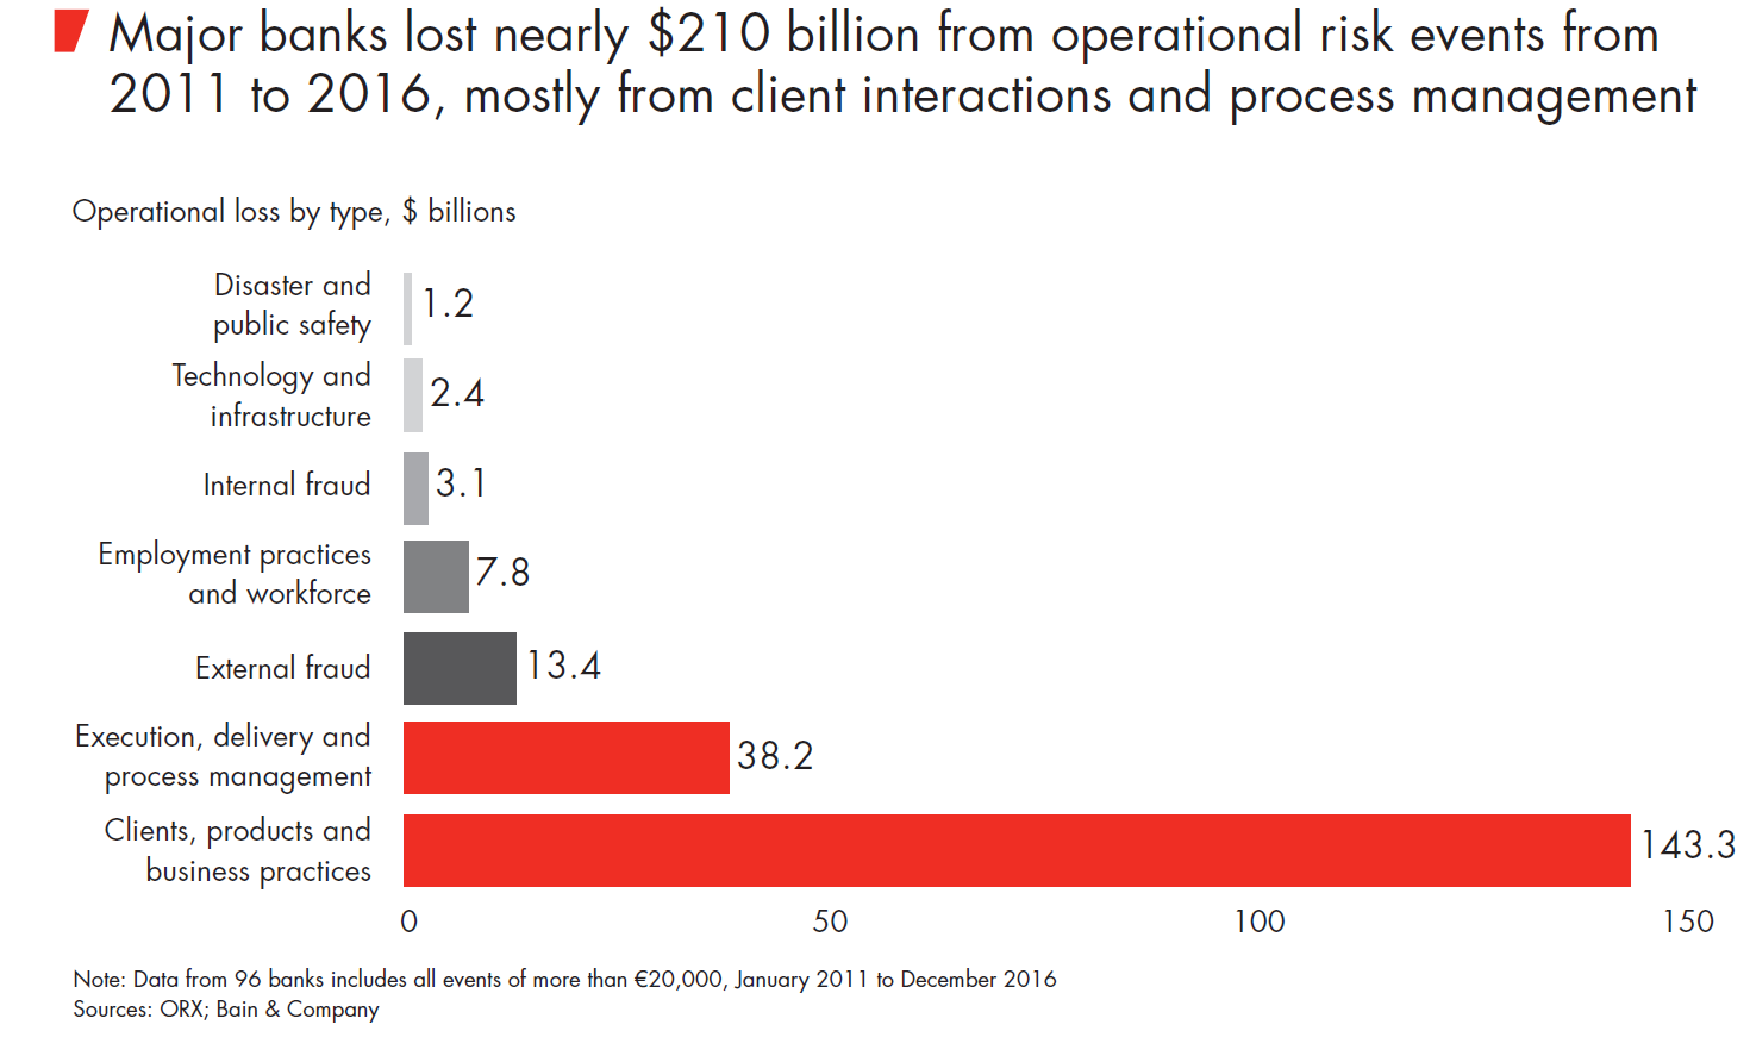
\includegraphics[width=15cm,height=8.0cm]{bank-oprisk_fig1_full.pdf}}
             {Source: \url{https://www.bain.com/contentassets/f0199ad9887e402cb37cd1fd316f5ee3/bain_brief_how_banks_can_manage_operational_risk.pdf}}
\caption[Losses suffered from 2011 to 2016 from Oprisk]{Histogram showing a breakdown of gross losses focusing on OpRisk loss events in comparison to each other recorded from 2011 up to and including 2016}
\label{bank-oprisk_fig}
\end{figure}

These OpRisk loss events were due to fraudulent trading activity
consisting of rogue traders dealing in illegally placed high frequency
trades for private clients where prices are hidden. For example, the
January 2016 \lq\lq Dark Pool\rq\rq~trading penalties suffered by
Barclays Bank PLC amounting to about \$70mn and Credit Suisse (\$85mn),
imposed by the United States (US) based securities exchange commision
(SEC). In a case closer to home, Gous (2019) reports ongoing
investigations launched in April 2015 for price fixing and
``widespread'' collusion between banking insiders in South Africa (SA),
of the market allocation for foreign exchange (FX) currency pairs viz.,
USD/ZAR rates, a case which now has been referred to SA based
competition tribunal for prosecution, as late as February 2017. Three
local banks viz., Absa bank, Standard bank \& Investec are implicated in
the scandal along with 14 others; some of which have already been fined
within juristictions they reside (StaffWriter, 2017), may be liable to
payment of an admistrative penalty equal to 10\% of their annual
turnover.\medskip

This investigation led by the local based competition commission
uncovered irregularities when rogue traders manipulated the price of the
rand through buying and selling US dollars in exchange for the rand at
fixed prices between 2007 and 2013. According to the competition
commission, currency traders allegedly had been colluding or
manipulating the price of the rand through these buy and sell orders to
change supply of the currency in contravention of the competition act
(Gous, 2019).\medskip

These acts compromise risk management's advisory service and pedigree,
and arouse huge interest as, with the SA incident, distorting the rand
value has major implications on the living standards of SA's, felt down
to the man in the street. Furthermore, this kind of behaviour can lead
to catastrophic operational losses resulting is a mismatch between
business' expectations and the value the risk management practice is
delivering, which is prevalent across the world and remains unchanged.
There are many attitudes that can potentially infect organisational
processes, the most persistent of these attitudes stem from human
failings that are exploitable (Barberis \& Thaler, 2003); such as the
human conditions' propensity to being deceitful during periods of
distress, thus forming a the basis for a (behavioural) theoretical
foundation of OpRisk management.

\section{The basel committee operational risk management framework}
\label{sec:The basel committee operational risk management framework}

The Bank for International Settlements (BIS) is an organisation
consisting of a group of central bank governors and heads of supervision
of central banks around the world who represent an authority on good
risk management in banking. More specifically, the BIS oversee the
duties of the Basel Committee on Banking Supervision (BCBS)/Basel
Commitee. The role of the BCBS is to set out guidelines on international
financial regulation to cover risks in the banking sector. There are to
date three banking accords from the BCBS under the supervision of the
BIS in dealing with financial regulation viz., Basel I, Basel II \&
Basel III. These accords describe an overview of capital requirements
for financial institutions (FI's) in order to create a level playing
field, by making regulations uniform throughout the world.

\subsection{The Capital Adequacy Accord (Basel I)}

Basel I was established in 1988. Basel I meant that FI's were required
to assign capital for credit risk to protect against credit default. In
1996, an amendment to Basel I imposed additional requirements to cover
exposure due to market risk as well as credit risks. Basel I effectively
minimised rules that favoured local FI's over potential foreign
competitors by opening up global competition so that these banks could
buffer against international solvency. In 2001, the Risk (2001)
consultative package provided an overview of the proposed framework for
regulatory capital (RC) charge for OpRisk upon the realisation of
financial institutions' (FIs) OpRisk component, which constitutes a
substantial risk component other than credit and market risk. \medskip

A construct for credit risk modelling uses in OpRisk is borne out of the
structural model found in Merton (1974), whereby a theory for pricing
corporate debt is presented. Merton (1974) postulates the bond's value
is dependent on the volatility of the firms value at a given interest
rate i.e., the risk structure of interest rates (Rosa, 2012) under
possible gains or losses to investors when there is a significant
(unanticipated) probability of default. This credit risk model adapted
to OpRisk defines what is now called the \emph{exposure-based} operation
risk (EBOR) model. The ultimate task of defining the ideal
\emph{exposure} measure for a operational event data is specifically
dealt with in this study.\medskip

The main challenge in OpRisk modeling is poor data quality and usually
very few data points that are often characterised by high frequency low
severity (HFLS) and low frequency high severity (LFHS) data types.
OpRisk's LFHS are risks where the probability of an extreme loss is very
small but costly, and HFLS risks are where frequency plays a major role
in the OpRisk capital charge calculation. It is common knowledge that
HFLS losses at the lower end of the loss spectrum tend to be ignored by
management due to their perceived insignificance and are therefore less
likely to be reported, whereas LFHS losses comprise of sensitive company
information, hence more than not are well guarded and kept in secret by
organisations, and therefore are not likely known to the public. Many
times losses of operational nature are mistakenly attributed to credit
defaults or market risk related movement.\medskip

This is founded in a seminal paper by Rosa (2012), through her
illustration of modern risk exposure whereby the afore-mentioned
phenomena arises: An exposure-based method is derived using a credit
risk structural model to predict a series of operational losses arising
from events of operational nature; which triggered off the filing of
litigations involving initial public offerings (IPO's), but nevertheless
related to credit or market risk losses as defined by the credit risk or
market risk exposures as opposed to standard OpRisk types whose exposure
was undefined. In fact, a significant gap in OpRisk literature is in the
current lack of a strongly risk-sensitive \emph{exposure} measure
(cf.~market and credit risk) (Aue \& Kalkbrener, 2006).\medskip

In an adaptation of the Merton (1974)'s concept to OpRisk as illustrated
by Rosa (2012) to OpRisk losses involving these IPO's, an EBOR model
emerges out of a method which requires new types of data incorporating
``predictive'' factors by the use of a combination of statistical
modeling and scenario analysis: Thus, allowing for the inclusion of
forward-looking aspects of BEICF's in an EBOR model. An early
representation of this EBOR model according to Rosa (2012) is expressed
as a common credit risk model given as:\medskip

\singlespacing

\begin{equation}\label{EBORmethod}
EL = p \cdot LGE 
\end{equation} \doublespacing

Where \(EL\) is the expected loss, \(p\) is the probability of the
realised loss occuring, and \(LGE\) is the loss-given-event. Oprisk
events are divided into event types \(ET_j\) \(j=1,2,\ldots\) and
business lines \(BL_i\) \(i=1,2,\ldots\). Other necessary inputs are:
the severity exposure \(E_{ij}\), or the maximum possible loss for an
event in the BL/ET combination risk cell \(ij\), an exposure indicator
capturing the scale of the bank's activities in the risk cell; and a
stochastic estimate \(L_{ij}\) specified since only a fraction of the
exposure is typically lost, such that \(LGE =L\cdot E\). Now, suppose
\(Y_{ij}\) denotes loss for business line \(BL_i\) \(i=1,2,\ldots\) and
event type \(ET_j\) \(j=1,2,\ldots\) for BL/ET combination \(ij\); and
\(p_{ij}\) denotes the probability that the OpRisk event will occur over
the next period \([T,T+\tau]\), then the total loss \(Y_{ij}\) is given
by:

\singlespacing

\begin{eqnarray}\label{EBORmethodology}
Y_{ij} = p_{ij} \cdot L_{ij} \cdot E_{ij} \qquad \mbox{where} \quad LGE = L \cdot E \quad \mbox{by}\quad \ref{EBORmethod}
\end{eqnarray} \doublespacing

Conceptually, this factor based quantification model for capital
requirements can be extended to also include future events.

\subsection{New Capital Adequacy Accord (Basel II)}

The framework for Basel II was implemented in June 2006. The rationale
for Basel II is to introduce risk sensitivity through more restrictive
capital charge measures and flexibility with specific emphasis on
OpRisk. The structure of the new accord is built upon a three-pillar
framework: Pillar I stipulates minimum capital requirements for the
calcualtion of regulatory capital for credit risk, market risk and
OpRisk in order to retain capital to ward against these risks. Pillar II
imposes a supervisory review process whereby additional capital
requirements can be imposed; such as the bank's internal capital
assessements or to act on needed adequate capital support or best
practice, for mitigating their risks. Pillar III relates to market
discipline i.e., transparency requirements which require banks to
publicly provide risk disclosures to keep them in line by enabling
investors to form an accurate view of their capital adequacy, in order
to reward or punish them on the basis of their risk profile.\medskip

Basel II describes three methods of calculating capital charge for
OpRisk RC viz., the standardised approach (SA), the basic indicator
approach (BIA) and the internal measurement approach (IMA). The basic
indicator approach (BIA) sets the OpRisk RC equal to a percentage (15\%)
of the annual gross income of the firm as a whole to determine the
annual capital charge. The SA is similar to the BIA except the firm is
split into eight business lines and assigned a different percentage of a
three year average gross income per business line, the summation of
which is the capital charge (Hoohlo, 2015). In the IMA, the bank uses
it's own internal models to calculate OpRisk loss.

\subsubsection{Internal measurement approach (IMA)}
\label{sssec:Internal measurement approach}

The internal measurement approach (IMA) allows banks to use their
internally generated risk estimates, Under Basel II the IMA is a first
attempt at capital charge calculation for OpRisk: ``to directly capture
a bank's underlying risk by using the bank's internal loss data as key
inputs for capital calculation'' (Mori, Harada, \& others, 2001). It has
similarities to the Basel II model for credit risk, where a loss event
is a default in the credit risk jargon. Under the IMA, OpRisk events are
divided into seven event types \(j=1,\ldots,7\) and eight business lines
\(i=1,\ldots,8\) (Risk, 2001) forming a loss decomposition of \(56\)
BL/ET combination sub-risks. Total capital charge is computed
as:\medskip

\singlespacing

\begin{eqnarray}\label{Internalmeasurement}
\mathcal{\Large{C}}_{OpRisk}^{IMA} &=& \sum_{i=1}^8 \sum_{j=1}^7 \gamma_{ij}\epsilon_{ij} \\
where \quad \epsilon_{i}&:& \quad \mbox{is the expected loss for business line $i$, risk type $j$} \nonumber \\
    \mbox{and} \quad  \gamma_{ij}&:& \quad \mbox{is an internal scaling factor} \nonumber\\
\Leftrightarrow \epsilon_{ij} \equiv Y_{ij} &=& p_{ij} \cdot L_{ij} \cdot E_{ij} \quad \mbox{from}\quad \ref{EBORmethodology}\nonumber\\
\end{eqnarray} \doublespacing

The scaling factor \(\gamma_{ij}\) represents a regulatory parameter
that is used to transform \(Y_{ij}\) into a capital charge. At its most
basic level, the EBOR model is a special case of the IMA.

\subsubsection{The BL/ET combination matrix}

The 3-dimensional diagram depicts the formation of a \(7 \times 8 = 56\)
BL/ET combination of matrix risk-type cells: A duration parameter
denoted by time \([T,T+\tau]\) representing the next period's loss
(usually the next year's annual loss) over which RC is defined is shown
along the depth \(k\) ordinate.

\begin{figure}\label{BL/ET Matrix}
\begin{tikzpicture}[every node/.style={minimum size=0.5cm},on grid]
\begin{scope}[every node/.append style={yslant=-0.5},yslant=-0.5]
  \shade[right color=gray!10, left color=black!50](0,0) rectangle +(8,8);
  \node at (0.5,7.5) {$\textbf{\mbox{BL}1}$};
  \node at (0.5,6.5) {$\color{green}{{X^l}_{11}}$};
  \node at (1.5,7.5) {$\textbf{\mbox{BL}2}$};
  \node at (2.5,7.5) {$\textbf{\mbox{BL}3}$};
  \node at (3.5,7.5) {$\textbf{\mbox{BL}4}$};
  \node at (4.5,7.5) {$\textbf{\mbox{BL}5}$};
  \node at (5.5,7.5) {$\textbf{\mbox{BL}6}$};
  \node at (6.5,7.5) {$\textbf{\mbox{BL}7}$};
  \node at (7.5,7.5) {$\textbf{\mbox{BL}8}$};
  \node at (7.5,6.5) {$\color{blue}{{X^l}_{18}}$};  
  \draw (0,0) grid (8,8);
\end{scope}   
\begin{scope}[every node/.append style={yslant=0.5},yslant=0.5]  
  \shade[right color=gray!70,left color=gray!10](8,-8) rectangle +(8,8);
  \node at (11.5,-0.5) {$\mathbf{\mbox{T}+\tau} \quad \Huge{\color{magenta}\xrightarrow{\hspace*{4cm}}}$};
  \node at (8.5,-1.5) {\textbf{ET1}};
  \node at (8.5,-2.5) {\textbf{ET2}};
  \node at (8.5,-3.5) {\textbf{ET3}};
  \node at (8.5,-4.5) {\textbf{ET4}};
  \node at (8.5,-5.5) {\textbf{ET5}};
  \node at (8.5,-6.5) {\textbf{ET6}};
  \node at (8.5,-7.5) {\textbf{ET7}};
  \node at (10.5,-1.5) {\mbox{ \scriptsize Internal Fraud}};
  \node at (10.5,-2.5) {\mbox{ \scriptsize External Fraud}};
  \node at (12.5,-3.5) {\mbox{ \scriptsize Employment Practices and Workplace Safety}};
  \node at (12.0,-4.5) {\mbox{ \scriptsize Client Products and Business Practices}};
  \node at (11.5,-5.5) {\mbox{ \scriptsize Damage to Physical Assets}};
  \node at (12.0,-6.5) {\mbox{ \scriptsize Business Disruption and System Failure}};
  \node at (12.5,-7.5) {\mbox{ \scriptsize Execution, Delivery and Process Management}};
\end{scope}   
\begin{scope}[every node/.append style={yslant=0.5,xslant=-1},yslant=0.5,xslant=-1]
  \node at (10.0,7.5) {\mbox{ \scriptsize Corporate Finance}};
  \node at (10.0,6.5) {\mbox{ \scriptsize Trading and Sales}};
  \node at (10.0,5.5) {\mbox{ \scriptsize Retail Banking}};
  \node at (10.0,4.5) {\mbox{ \scriptsize Commercial Banking}};
  \node at (10.0,3.5) {\mbox{ \scriptsize Payment and Settlement}};
  \node at (10.0,2.5) {\mbox{ \scriptsize Agency Services}};
  \node at (10.0,1.5) {\mbox{ \scriptsize Asset Management}};
  \node at (10.0,0.5) {\mbox{ \scriptsize Retail Brokerage}};
\end{scope}  
\end{tikzpicture}
\caption{The 3-Dimensional grid of the BL/ET matrix for 7 event types and 8 business lines}
\end{figure}

\subsection{Basel III}

Basel III establishes tougher capital standards through more restrictive
capital definitions, higher risk weighted
assets\footnote{Also reffered to as risk-weighted amount, it is a measure of the bank's total credit exposure}
(RWA's), additional capital buffers, and higher requirements for minimum
capital ratios (Dorval, 2013). Through Basel III, the BCBS is
introducing a number of fundamental reforms grouped under three main
headings (Committee \& others, 2010): 1{]} A future of more capital
through incremental trading book risk (credit items in trading book
treated in the same way as if they were in banking book), 2{]} More
liquidity through the introduction of a global liquidity risk standard:
Basel III will push banks toward holding greater levels of liquid
instruments, such as government bonds and more liquid corporate
instruments, and 3{]} Lower risk under the new requirements of the
capital base i.e., establish more standardized risk-adjusted capital
requirements.\medskip

The future regulatory environment requires OpRisk professionals who are
not only intelligent, creative and motivated but also have the courage
to uphold the OpRisk advisory service standards. Businesses that want to
successfuly manage OpRisk would be well advised to utilize new
theoretical and empirical techniques such that large and small scale
experiments play an important role in risk analysis and regulatory
research.

\section{Modern OpRisk measurement frameworks (ORMF's)}
\label{sec:Modern OpRisk measurement frameworks (ORMF's)}

Regarding the sequence Basel I and Basel II: Regulation begins as a
qualitative recommendation which requires banks to have an
assets-to-capital multiple of at least 20, then focuses on ratios in
which both on-balance sheet and off-balance sheet items are used to
calculate the bank's total RWA, then on tail risk. In other words,
auditors' discretion is replaced by market perception of capital,
meaning there is a market risk capital charge for all items in the
trading business line, then exciting new static risk management
approaches which involve calculating a 99.9 percentile left tail
confidence interval to measure OpRisk value-at-risk (VaR) and convert it
into a RC charge.\medskip

\subsection{Advanced Measurement Approach (AMA)}
\label{sec:Advanced Measurement Approach (AMA)}

The advanced measurement approach (AMA) is an IMA method which applies
estimation techniques of OpRisk capital charge derived from a bank's
internal risk measurement system (Cruz, 2002). Basel II proposed
measurement of OpRisk to define capital requirements against unexpected
bank losses whereas the unexpected loss (UL) is the quantile for the
level \(\alpha\) minus the mean. According to the AMA, which is thought
to outperform the simpler SA approach and the BIA, RC requirements are
defined according to the UL limit in one year and the loss distribution
at a 99.9\% confidence level (\(\alpha = 0.01\%\)) aggegate loss
distribution\footnote{The aggregate loss distribution is obtained by convoluting a loss event frequency distribution and a loss severity distribution by means of the random sums method.}
used as a measure of RC. The BCBS proposes to define RC as \(RC = UL\).
This involves simulations based on historical data to establish
frequency and severity distributions for losses. In this case the RC is
a VaR measure.\medskip

\subsubsection{Loss distribution approach (LDA)}
\label{sssec:Loss distribution approach (LDA)}

The loss distribution approach (LDA) model is based on actuarial
techniques and is generally accepted as the industry (AMA) standard for
OpRisk estimation. LDA models require quant level expertise in order for
one to accept the statistical relationships linking the actual
(perceived) risk exposures. What it has done is to provide the most
realistic risk profiles of a company to date (Einemann et al., 2018),
based on partitioning OpRisk loss data into sufficiently homgeneous
sets, typically corresponding to combinations of business lines (BL) and
event types (ET), and to calibrate a frequency and severity distribution
for each BL/ET combination.\medskip

LDA models cover risks that are well reflected through historical events
and exposure data is used in several of the steps of the process in
frequency and severity modeling. The risk-type cells can be selected at
the actual loss generating process level, however most banks use the LDA
for BL/ET risk-type cells. The LDA is the most comprehensive modelling
approach and is the focus of this study forthwith. \medskip

\subsection{What is exposure?}
\label{sec:What is exposure?}

In the OpRisk context, the total OpRisk loss is captured by certain
\emph{exposure} measures, which are quantities that are thought to be
roughly proportional to the overall risk associated with an operational
event or loss (Parodi, 2014). The measure of exposure needed depends on
what loss variable one is attempting at projecting which is dependent on
a varied mix of factors. Specifically in relation to the LDA model for
OpRisk the exposure measure is dependent on whether we are projecting
the aggregate losses (severity) or the number of losses (frequency).
When carrying out this decision making expercise the following were
considered:

\begin{list}{*}{}
\item The availability of historical exposure data over the same period for which the losses are recorded
\item The exposure estimate for future periods
\end{list}
\medskip

Exposure is residual risk, or the risk that remains after risk
treatments have been applied. In the ORMF context, it is defined as: The
formal definition of exposure in risk management is:

\subsubsection{Definition of exposure}
\label{sssec:Definition of exposure}
\begin{definition}
\emph{\textbf{The risk remaining after risk treaments have been applied}} i.e., the risk *a priori* to considering the actual experience of the corporation or FI. The  \textbf{exposure} of risk type $i$, $d_{i}$ is the time interval, expressed in units of time, from the initial moment when the event happened, until the occurrence of a risk correction.
\end{definition}

As per definition \ref{sssec:Definition of exposure}, the lag represents
exposure; we need historical exposure for experience rating because we
need to be able to compare the loss experience of different years on a
like-for-like basis and to adjust it to current exposure levels (Parodi,
2014).

\subsubsection{Definition of rate}
\label{sssec:Definition of rate}

Often the poisson count \(\lambda\) needs to be described as a rate; for
example the OpRisk hazard rate can be specified as the rate per day.
More generally, the rate is specified in terms of units of
\emph{exposure}; The \textbf{rate}, \(R\) is defined as:\medskip

\begin{definition}
the \textbf{rate} is the mean count per unit exposure
\end{definition}

i.e., \singlespacing \begin{eqnarray}
R &=& \frac{\mu}{\tau} \qquad \mbox{where} \qquad R = \mbox{rate,} \quad \tau = \mbox{exposure},d_{i}\quad \mbox{and}\nonumber\\
\mu &=& \mbox{mean count over an exposure duration of} \quad d = [T,T+\tau] \nonumber
\end{eqnarray} \doublespacing

For example, in OpRisk hazard rates, each potential OpRisk transaction
event is ``exposed'' over the period \([T,T+\tau]\); it's detection life
cycle period, and a P\&L impact determined, So the rate may be defined
in terms of transcaction-days \emph{at risk}. In this study, the
intensity (rate) of occurance of loss events is the fundamental unit of
of analysis for estimating the number of loss events (frequency) used
for OpRisk losses. This positions the Poisson distribution as a
favourable first model; and presents the researcher with the opportunity
for a intuitive intepretation of \emph{exposure} as the rate for
counting for all available observations over a time lag: The
\emph{\textbf{exposure}} measure is defined as the time interval
\((T+\tau,T) = \mbox{d}\) i.e., the interval from the initial moment
when the event happened until the moment the event is observed and
adjusted for.\medskip

The Basel III capital adequacy rules permit model-based calculation
methods for capital, including the AMA for OpRisk capital. Under Basel
III, standardised methods for OpRisk capital have been overhauled,
however for a while there was no prospect of an overhaul of the AMA.
Given the relative infancy of the field of OpRisk measurement, banks are
mostly free to choose among various AMA principle-based frameworks to a
significant degree of flexibility (Risk, 2016). A bank that undertakes
an AMA should be able to influence their capital requirements through
modeling techniques resulting in lowered pressure on OpRisk capital
levels, which in turn has a positive impact on the bank.\medskip

A FI's ability to determine the framework used for its regulatory OpRisk
RC calculation, evolves from how advanced the FI is along the spectrum
of available approaches used to determine capital charge (Risk, 2001).
BCBS recognizes that a variety of potentially credible approaches to
quantify OpRisk are currently being developed by the industry, and that
these R\&D activities should be incentivised. Increasing levels of
sophistication of OpRisk measurement methodologies should generally be
rewarded with a reduction in the regulatory OpRisk capital requirement.

\subsection{The standardised measurement approach (SMA)}

The flexibility of internal models was expected to narrow over time as
more accurate OpRisk measurement was obtained and stable measures of RC
were reached, ultimately leading to the emergence of best practice.
Instead, internal models produced wildly differing results of OpRisk RC
capital from bank to bank, contrary to the expectations of the BCBS. In
March 2016, the BCBS published for consultation a standardised
measurement approach (SMA) for OpRisk RC; that proposes to abandon the
freedom of internal modelling (thus ending the AMA) approaches for
OpRisk RC, in exchange for being able to use a simple formula to
facilitate comparability across the industry.\medskip

Under the SMA, RC will be determined using a simple method comprising of
two components: A stylised systemic risk model (business indicator
component), and an idiosyncratic risk model (loss component), which are
combined via an internal loss multiplier (ILM), whose function is to
link capital to a FI's operational loss experience to determine SMA
capital.\medskip

The SMA formula is thought to be consistent with regulators' intent for
simplification and increased comparability across most banks. However,
there is a feeling from some in the banking industry that the SMA is
disadvantaged as it is not the same as measuring OpRisk. Mignola,
Ugoccioni, \& Cope (2016) and Peters, Shevchenko, Hassani, \& Chapelle
(2016) identified that the SMA does not respond appropriately to changes
in the risk profile of a bank i.e., it is unstable viz., two banks of
the same risk profile and size can exibit OpRisk RC differences
exceeding 100\%, and risk insensitive; that SMA capital results
generally appear to be more variable across banks than AMA results,
where banks had the option of fitting the loss data to statistical
distributions.

\subsection{Argument}
\label{ssec:Argument}

Over the last twenty years, hard-won incremental steps to develop a
measure for the size of OpRisk exposure along with the emergence of
promising technologies presents a unique opportunity for bankers and
treasurers - traditionally risk-averse players - to develop a novel type
of way of looking at decision making under risk/uncertainty. New
technologies have been introduced which make use of up to date technical
solutions (such as homo heuristics developed by Gigerenzer \& Brighton
(2009), who mainatain their methods solve practical finance problems by
simple rules of thumb, or Kahneman (2003)'s intuitive judgements and
deliberate decision making), argued to more likely represent the true
embedded OpRisk in financial organisations as these methods are designed
to fit normal behavioral patterns in their formulation, which is
consistent with how decisions are made under risk/uncertainty.\medskip 

What are the important steps toward completing the post crisis reforms
during the current year? Should the risk management fraternity follow
the
chartered\footnote{Meaning as of the publication [@risk2016supporting] the methods brought forth in the consultative document have not been approved for the public, the ideas within an experimental (leased) phase for the exclusive use of BCBS and certain FI's}
path followed in the Risk (2016) consultative document, scrapping away
twenty years of internal measurement approaches (such as the AMA), or
should the focus of financial regulators shift toward improving on what
they see fit within current existing AMA frameworks. The question is
should OpRisk managements' focus be on stimulating active discussions on
practical approaches to quantify, model and manage OpRisk for better
risk management and improved controls, or abandon the adoption of
innovative measurement approaches, such as the AMA, in exchange for
being able to use a simple formula across the whole industry?

\section{Context of the study}
\label{sec:Context of the study}

Regulatory reforms are designed and fines imposed to protect against
operational errors and other conduct costs connected with wrongdoing and
employee misconduct. Despite the introduction and use of these seemingly
robust strategies, regulations, processes and practices relating to
managing risk in FI's, bank losses continue to occur at a rather
distressing frequency. A cyclical pattern of OpRisk loss events still
persists; as evidenced in the recent price fixing and collusion cases,
defeating the explicit objectives of risk management frameworks. This
demonstrates a scourge of reflexivity prevailing in financial markets
emphasising that, there are theories that seem to work for a time only
to outlive their use and become insufficient for the complexities that
arise in reality.

\subsection{Why \texttt{OpRisk?}}

A forceful narrative in management theory is that an organisation
running effective maintenance procedures combined with optimal team and
individual performers i.e., the right balance of skills in the labour
force and adequate technological advancements, means systems and
services can be used to more efficiently produce material gains, enhance
organisational effectiveness, meet business objectives and increase
investment activity. Conversely, the risk of the loss of business
certainty associated with lowered organisational competitiveness and
inadequate systems technology that underpins operations and services is
a key source leading to a potential breakdown in investment services
activity (Hoohlo, 2015).\medskip

In fact, OpRisk controls could set banks apart in competition. Consider
the case of a risk practitioner in a financial system who assumes that
he/she is consiously and accurately executing tasks and analysing an
observed subject trusting the validity and relying on visual information
that their sense of sight reveals alone. In the absence of visual
confirmation they are hindered from extracting and/or analysing
information about the system and their efforts to regulate could
potentialy fail. In this scenario, the organisational methods and
functioning of information systems would usually pose shortcomings,
which obscure the full extent of OpRisk challenges from the eyes of the
risk practitioner allowing for operational errors. \medskip

When an attack such as an operational error occurs at a speed that the
OpRisk agent (an individual legal entity or a group) is unable to react
quickly enough, due to limitations of their processing speed, and they
are not able to process all the information in the given time span, they
could lose control/fail of fail in compliance, disincentivising support
for regulation, particularly Basel III recovery and resolution
processes. In latter days more often than not, OpRisk loss cases reflect
lack of sufficient controls being the driver of current OpRisk
management catastrophies. The agent on this end of the spectrum of the
risk management strategy, which mitigates risk and enforces regulation
dependent on visual and information controls is better off than an agent
on the other extreme, who does not react at all to changes in the system
environment.

\section{A new class of EBOR models approach}
\label{sec:A new class of EBOR models approach}

In this study, an important new algorithm for ORMFs and is laid out
coupled with data intensive estimation techniques; viz.~Generalised
Additive Models for locatin Scale \& Shape (GAMLSS), Generalized Linear
Models (GLMs), Artificial Neural Networks (ANNs), Random Forest (RF) \&
Decision Trees (DTs), which have capabilities to tease out the deep
hierarchies in the features of covariates irrespective of the challenges
associated with the non-linear or multi-dimensional nature of the
underlying problem, at the same time supporting the call from industry
for a new class of EBOR models that capture forward-looking aspects.

\section{Problem statement}
\label{sec:Problem statement}

\subsection{Main problem}
\label{ssec:Main problem}

Conventional OpRisk frameworks in banking commonly exhibit control and
system deficiencies whereby information processing is slow and have the
tendency to rely on manual, uncertain, unpredictable and unrealistic
management and measurement methods, obscuring reporting and resulting in
undesirable pre-market conditions. The OpRisk management's function
should be able to assist in the ability to mitigate risks through
acquiring and/or refining risk management solutions which deliver
reliable and consistent benefits of improved operational controls and
enhanced risk management frameworks.\medskip

In our prevailing banking phenomena of increasing OpRisks, the problem
consists of questioning whether a firm's susceptibility to OpRisk
hazard's growth, results in the degree of OpRisk losses slowing due to
tightning OpRisk controls and enhancements to OpRisk frameworks. It
would be prudent not to declare things are improving if the evidence is
not quite firm that this is true. This is essentially a check for
situations, from these data, whether there is evidence of the unchecked
spread of negligent behaviour leading to operational loss events or not;
or on the contrary, those situations other than the unrestricted spread
of these ``rogue'' events conscequently driving OpRisk losses i.e.,
which may requiring a re-thinking our approach to improving OpRisk
controls and enhancing OpRisk management frameworks.

\subsubsection{Sub-problem 1}
\label{sssec:Sub-problem 1}

The existing models in OpRisk measurement for which historical loss
distributions are the best predictors of future losses, assume that we
do not learn from past losses. This is problematic for ``predictable''
risk types due to model's practice of undercapitalising known risks
before occur, and overcapitalising for risks after the losses
materialise, creating innappropriate capital estimates (Group \& others,
2013). These concerns motivate the development of an EBOR modelling
framework which not only captures past losses but also how exposures to
forward-looking affect risk attitudes.

\subsubsection{Sub-problem 2}
\label{sssec:Sub-problem 2}

Furthermore, we challenge the weakness in current OpRisk theory which
assumes banks are risk neutral, asserting they are more risk averse.
Consequently, ``predictive'' future losses can be determined who's
estimated RC adapts to changes in the risk profile of the bank i.e.,
with the introduction of new products or in changes to the business mix
of the portfolio (e.g.~mergers and aquisitions, trade terminatons,
allocations or disinvestments), providing sufficient incentives for
OpRisk management to mitigate risk.

\section{Objectives of the study}
\label{sec:Objectives of the study}

The research objectives are three-fold:

\subsection{Exposure-based OpRisk (EBOR) models}

To quantify OpRisk losses by introducing generalised additive models for
location, scale and shape (GAMLSS) in the framework for OpRisk
management, that captures exposures to forward-looking aspects of the
OpRisk loss prediction problem. EBOR treatments effectively replace
historical loss severity curves obtained from historical loss counts, by
looking into deep hierarchies in the features of covariates in
investment banking (IB), and by forward-looking measures using event
frequencies based on actual operational risk (OpRisk) exposures in the
business environment and internal control risk factors (BEICF) thereof.

\subsection{Modeling OpRisk depending on covariates}

To investigate the performance of several supervised learning classes of
data-intensive methodologies for the improved assessment of OpRisk
against current \emph{traditional} statistical estimation techniques.
Three different machine learning techniques viz., DTs, RFs, and ANNs,
are employed to approximate weights of input features (the risk factors)
of the model. A comprehensive list of user defined input variables with
associated root causes contribute to the \emph{frequency} of OpRisk
events of the underlying value-adding processes. Moreover, the
\emph{severity} of OpRisk is also borne out through loss impacts in the
dataset . As a consequence of theses new mwthodologies, capital
estimates should be able to adapt to changes in the risk profile of the
bank, i.e.~upon the addition of new products or varying the business mix
of the bank providing sufficient incentives for ORMF to mitigate risk
(Einemann et al., 2018).

\subsection{Interpretation Issues using cluster analysis}

To identify potential flaws in the mathematical framework for the loss
distribution approach (LDA) model of ORM, which is based the derivation
of OpRisk losses based on a risk-neutral measure \(\mathbb{Q}\), by
employing Cluster Analysis (CA). The study addresses weaknesses in the
current \emph{traditional} LDA model framework, by assuming managerial
risk-taking attitudes are more risk averse. More precisely, CA learns
the deep hierarchies of input
features\footnote{A typical approach taken in the literature is to use an unsupervised learning algorithm to train a model of the unlabeled data and then use the results to extract interesting features from the data [@coates2012learning]}
that constitute OpRisk event \emph{frequencies} \& \emph{severities} of
losses during banking operations.\medskip

In theory, a risk manager who experiences persistent/excessive losses
due to particular risk events, would over-compensate cover for these
particular risk types. This would show in reduced losses in those loss
event types over time, subsequently determining whether risk adverse
techniques over-compensate for persistent losses. The wish is to bring
the prescribed model to equilibrium by applying a method that tries to
establish what accurately ascribes to decision rules that people wish to
obey in making predictions about what operational loss events might
result in the future, then use empirical data to test this idea in a way
that is falsifyable.

\section{Significance of the study}
\label{sec:Significance of the study}

This study fills a gap in that advancing OpRisk VaR measurement methods
beyond simplistic and traditional techniques, new data-intensive
techniques offer an important tool for ORMFs and at the same time
supporting the call from industry for a new class of EBOR models that
capture forward-looking aspects of ORM (Embrechts, Mizgier, \& Chen,
2018). The current \emph{traditional} approach consists of a loss data
collection exercise (LDCE) which suffers from inadequate technologies at
times relying on spreadsheets and manual controls to pull numbers
together, and therefore do not support the use of data intensive
techniques for the management of financial risks. In this study, a new
dataset with unique feature characteristics is developed using an
automated LDCE, as defined by Committee \& others (2011) for internal
data. The dataset in question is at the level of individual loss events,
it is fundamental as part of the study to know when they happened, and
be able to identify the root causes of losses arising from which OpRisk
loss events.\medskip 

This study will provide guidance on combining various supervised
learning techniques with extreme value theory (EVT) fitting, which is
very much based on the Dynamic EVT-POT model developed by
Chavez-Demoulin, Embrechts, \& Hofert (2016). This can only happen due
to an abundance of larger and better quality datasets and which also
benefits the loss distribution approach (LDA) and other areas of OpRisk
modeling. In Chavez-Demoulin et al. (2016), they consider dynamic models
based on covariates and in particular concentrate on the influence of
internal root causes that prove to be useful from the proposed
methodology. Moreover, EBOR models are important due to wide
applicability beyond capital calculation and the potential to evolve
into an important tool for auditing process and early detection of
potential losses, culminating in structural and operational changes in
the FI, hence releasing human capital to focus on dilemmas that require
human judgement.

\section{Organisation of the study}
\label{sec:Organisation of the study}

This study consists of seven chapters. Chapter \ref{INTRODUCTION}
outlines the purpose, followed by an overview of the relevance and
importance in the existing work. Then the general concept behind EBOR
models is introduced and an argument is presented of the relevance of a
new class of EBOR models to remediate some of the shortcomings in OpRisk
LDA modeling, followed by statement of the research problems and
objectives. This chapter is concluded by an account of
significance.\medskip

The introductory chapter is succeded by a general literature review
Chapter \ref{LITERATURE REVIEW}, succeeded by three stand alone
chapters, the purpose of each is to provide clarity, based on theory and
empirical evidence, focusing on three specific research objectives each
contributing to resolve specific problems in the OpRisk literature,
given how its importance has become more pronounced in time. In these
chapters the application of machine learning techniques on the observed
data take centre-stage demonstrating how issues in OpRisk capital
requirement estimation are more effectively resolved.\medskip

Chapter \ref{LITERATURE REVIEW} gives an overview of theoretical
foundations of OpRisk, followed by a review of the LDA model used to
calculate an estimate of the OpVaR measure. A breakdown analysing the
EBOR models approach follows promising to remediate some of the LDA
shortcomings and on how EBOR components presented in the study offer a
novel approach in contrast to the current literature demonstrating its
value and exposing the gap in finer detail. Chapter
\ref{LITERATURE REVIEW} concludes with a lead up to Chapter
\ref{EXPOSURE-BASED OPERATIONAL RISK ANALYSIS} by proposing a research
methodology in which a combination of ML techniques and statistical
theory underlying ORMF's would benefit measurement of capital
requirements for OpVaR.\medskip

Chapter \ref{EXPOSURE-BASED OPERATIONAL RISK ANALYSIS} deals with the
application of EBOR techniques using the GLM and GAMLSS models in more
detail, and the empirical determinants due to the different components
of OpRisk measurement under the new class of EBOR models. The chapter
deals with the analysis of EBOR techniques to the portfolio of a wide
range OpRisk losses found in the dataset and their integration into an
LDA framework.

\FloatBarrier
\newpage
\fancyhead[L]{Literature Review}
\fancyhead[R]{\thepage}
\fancyfoot[C]{}

\chapter{LITERATURE REVIEW}
\label{LITERATURE REVIEW}

\doublespacing

\section{Introduction}
\label{sec2:Introduction}

A look into literary sources for OpRisk indicates (Acharyya, 2012) that
there is insufficient academic literature that looks to characterize its
theoretical roots, as it is a relatively new discipline, choosing
instead to focus on proposing a solution to the quantification of
OpRisk. This chapter seeks to provide an overview of some of the
antecedents of OpRisk measurement and management in the banking
industry. As such, this chapter provides a discussion on why OpRisk is
not trivial to quantify and attempts to understand its properties in the
context of risk aversion with the thinking of practitioners and
academics in this field.\medskip

According to Cruz (2002), FI's wish to measure the impact of operational
events upon profit and loss (PnL), these events depict the idea of
explaining the \emph{volatility of earnings} due to OpRisk data points
which are directly observed and recorded. By seeking to incorporate new
data intensive machine learning (ML) approaches to help understand the
data, the framework analyses response variables that are decidedly
non-normal, including categorical outcomes and discrete counts.\medskip

Due to commonly held beliefs (Aue \& Kalkbrener, 2006), one of the main
challenges toward the next generation of LDA models is in their
incapability of dealing with the handling of statistical validation of
qualitative adjustments, citing ill-conceived justification for its
direct application to RC: However, in the advent of recent developments
.viz ML techniquess, it is believed the advantages of conducting our
investigations outweigh this disadvantage, shedding further light on our
understanding of how forward-looking aspects of BEICF's affect
firm-level OpRisk RC. Lastly, this resolves the problem associated with
the context dependent nature of OpRisk as an apparent gap in the
literature.

\section{The theoretical foundation of OpRisk}
\label{sec:The theoretical foundation of OpRisk}

Hemrit \& Arab (2012) argue that common and systematic operational
errors in hypothetical situations poses presumtive evidence that OpRisk
events, assuming that the subjects have no reason to disguise their
preferences, are created sub-consciously. This study purports, supported
by experimental evidence behavioural finance theories should take some
of this behaviour into account when trying to explain in the context of
a model, how investors maximise a specific utility/value
function.\medskip

In a theoretical paper, Wiseman \& Catanach Jr (1997) discussed several
organizational and behavioural theories, such as prospect theory (PT),
which influence managerial risk-taking attitudes. Their findings
demonstrate that behavioural views, such as PT and the behavioural
theory of the firm explain risk seeking and risk averse behaviour in the
context of OpRisk even after agency based influences are controlled for.
Furthermore, they challenge arguments that behavioral influences are
masking underlying root causes due to agency effects. Instead they argue
for mixing behavioral models with agency based views obtaining more
complete explanations of risk preferences and risk taking behavior
(Wiseman \& Catanach Jr, 1997). \medskip

Wiseman \& Catanach Jr (1997) suggest that managerial risk-taking
attitudes are influenced by the decision (performance) context in which
they are taken. In essence, managerial risk-taking attitude is
considered as a proxy for measuring OpRisk (Acharyya, 2012). In so
doing, Wiseman \& Catanach Jr (1997) investigate more comprehensive
economic theories viz.~PT and the behavioural theory of the firm, that
prove relevant to complex organizations who present a more fitting
measure for OpRisk. Upon further investigation, Barberis \& Thaler
(2003) reveal that in finance, behavioral theory explains whether
certain financial phenomena can be viewed as the result of less than
fully rational thinking. Their argument goes, that through integrating
OpRisk management into behavioral theory it may be possible to improve
our understanding of firm level RC by refining the resulting OpRisk
models to account for these behavioral traits. Thus implying that
people's economic preferences described in the model have an economic
incentive to improve the OpRisk RC measure. \medskip

Despite the reality that OpRisk does not lend itself to scientific
analysis in the way that market risk and credit risk do, someone must do
the analysis, value the RC measurement and hope the market reflects
this. Besides, financial markets are not objectively scientific, a large
percentage of successful people have been lucky in their forecasts, it
is not an area which lends itself to scientific analysis.

\section{Overview of operational risk management}
\label{sec:Overview of operational risk management}

It is important to note how OpRisk manifests itself: The causes and
sources of operational loss events as observed phenomena associated with
operational errors and are wide ranging (King, 2001). By definition, the
occurence of a loss event is due to PnL volatitlity from a payment,
settlement or a negative court ruling within the capital horizon over a
time period (of usually one year) (Einemann et al., 2018). As such, PnL
volatitlity is not only related to the way firms finance their business,
but also in the way they \emph{operate}.\medskip 

In operating practice, one assumes that on observing or on following
instructions we are consciously analysing and accurately executing our
tasks based on the information available. However, the occurence of
operational loss events indicates that there are sub-concious faults in
information processing, which we are not consciously aware of but
ultimately lead to PnL losses. These operational loss events are almost
always initiated at the dealing phase of the investment banking process;
which more often than not implicates front office (FO) personnel who
bear the brunt of responsibility for the loss e.g., during the trading
process in cases where OpRisk events occur as a result of a mismatch
between the trade booked (booking in trade feed) and the details agreed
by the trader.\medskip

The middle office (MO) and back offices (BO) conduct OpRisk managements'
task of building mathematical models to be used to predict OpRisk losses
and ultimately determine capital adequacy required to absorb these
losses. The implications from modelling can be used to better understand
the broad view of the overall company's OpRisk exposure, through PnL
attribution carried out from deal origination to settlement. For
instance, the results of the model can be used to better understand the
interrelationships between risk factors and potential dependencies on
various mitigation and management strategies (Acharyya, 2012) e.g.,
human error is a potential risk factor resulting PnL losses, whose
negative impacts can be mitigated by an efficient trade amendment policy
offsetting the outflow of PnL with an equal and opposite inflow or cash
injection.\medskip

Furthermore (Acharyya, 2012), organizations may hold OpRisk due to
external causes such as failure of third parties or vendors (either
intentionally or unintentionally) in maintaining promises or contracts.
The criticism in the literature is that no amount of capital is
realistically reliable for the determination of RC as a buffer to
OpRisk, particularly the effectiveness of the approach of capital
adequacy from external events as there is effectively no control over
them.\medskip

\section{The loss collection data exercise (LCDE)}
\label{sec:The loss collection data exercise (LCDE)}

In this study, a new dataset with unique feature characteristics is
developed using the official loss data collection exercise (LDCE), as
defined by Committee \& others (2011) for internal data. The dataset in
question is at the level of individual loss events which can therefore
be modelled in a granular way, which facilitates the reflection of
loss-generating mechanisms (Einemann et al., 2018): It is therefore also
fundamental as part of this study to know when they happened, and be
able to identify the root causes of losses arising from which OpRisk
loss events. Similarly to the afore-mentioned, this study intoduces an
analogous mathematical framework for EBOR modeling, however the proposed
OR framework is better suited with a higher probability to determine the
amount of capital necessary to absorb operational losses as it is
applicable to a larger number of OpRisk types.\medskip

The LCDE is carried out drawing statistics directly from the trade
generation and settlement system, which consists of a tractable set of
documented trade detail extracted at the most granular level, i.e.~on a
trade-by-trade basis (as per number of events (frequencies) and
associated losses (severities)) and then aggregated daily. The
development, calibration and validation of EBOR models is challenginf
since new types of data and ahigher degree of expert involvement acroos
the institution is required, providing a transparent quantitative
framework for combining forward-looking point-in-time data and
historical loss experience (Einemann et al., 2018). The afore-mentioned
LDCE is an improved reflection of the risk factors by singling out the
value-adding processes associated with individual losses on a
trade-by-trade level. The dataset is then split into proportions and
trained, validated and tested.

\section{Loss Distribution Approach (LDA)}
\label{sec:Loss Distribution Approach (LDA)}

The Loss Distribution Approach (LDA) is an AMA method whose main
objective is to provide realistic estimates to calculate VaR for OpRisk
RC in the banking sector and it's business units based on loss
distributions that accurately reflect the frequency and severity loss
distributions of the underlying data. Having calculated separately the
frequency and severity distributions, we need to combine them into one
aggregate loss distribution that allows us to produce a value for the
OpRisk VaR. \medskip

\subsection{A general class of LDA model characteristics}

We begin by defining some concepts:

\begin{itemize}
\item Consider a matrix consisting of business lines $BL$ and OpRisk event types $ET$. In line with Basel II, the bank estimates for each business line/event type (BL/ET) combination, the probability function (p.f.) of a single event severity\footnote{refers to the PnL impact resulting from the frequency of events} (PnL impact) and the event frequency\footnote{refers to the number of events that occur within the specified time period (daily buckets) $T$ and $T + \tau$} over a period, say for the next three months according to @hoohlo2015new. More precisely, according to @frachot2001loss, in each cell of the BL/ET matrix combinations separate distributions for loss frequency and loss severity are modeled and following an actuarial approach aggregated to produce a loss distribution at the group level.

\item More precisley, let $N_1,\ldots,N_m$ represent random variables for the loss frequencies i.e., the values $N_k \in \mathbb{N_{>0}}$ for each $k \in \{1,\ldots,m\}$. Let the individual operational losses \begin{math} (S_{k1}, \ldots, S_{kN_k})\end{math} denote independent and identically distributed (i.i.d) rv's of the severity distribution $S_k$, which are independent of $N_k$, be samples obtained from BL/ET combination types $k$. The aggregate loss variable $X_k$ in this cell is given as

\singlespacing
\begin{equation}\label{AggLossVar}
X_k = \sum_{l=1}^{N_k}S_{kl} 
\end{equation}
\doublespacing

The aggregate OpRisk loss can be seen as a sum $\mathbf{X} = X_1 + X_2 + \cdots + X_m$; the aggregate loss distribution at group level defined by

\singlespacing
\begin{eqnarray}\label{CombLossVar}
\mathbf{X} &=& \sum_{k=1}^m X_k \\
           &=& \sum_{k=1}^m \sum_{l=1}^{N_k}S_{kl} \quad \mbox{by equation} \ref{AggLossVar}
\end{eqnarray}
\doublespacing

\item Three month daily statistics are taken of the time series of internal processing errors (frequency data) and their associated severities and used in each cell of the BL/ET matrix. Daily buckets are chosen in order to ensure data points are sufficient for ML/statistical analysis.
\end{itemize}

\subsection{Computing the frequency distribution}
\label{ssec:Computing the frequency distribution}

\begin{itemize}
\item $\mathbf{N}_{ij}$ represents the number of times of OpRisk event failures between times $T$ \& $T +\tau$ in BL/ET combination $ij$, where subscripts $i$ refers to the $BL$ and $j$ to $ET$. More generally the rv $N_{k}$\footnote{$N_1 = N_{ij}$, where subscript $i=1$ \& $j=1$ i.e., $N_{11}$ corresponds to dealing with $ET_1$ e.g., internal Fraud and $BL_1$ e.g., Corporate Finance} has distribution function (d.f)\footnote{The term distribution function (d.f) is monotonic increasing function of $n$ which tends to $0$ as \begin{math} n \Longrightarrow -\infty\end{math}, and to $1$ as \begin{math} n \Longrightarrow \infty \end{math}} \begin{math}\mathbf{P}_{k}(n/\theta_0)  \end{math}, where $\theta_0$ is an unknown parameter to be estimated in some way, the two best known methods used are the maximum likelihood estimators (m.l.e) or the method of moments.\medskip

\item The d.f. \begin{math}\mathbf{P}_{k}(n/\theta_0)  \end{math} for the loss frequency, is defined as the probability that $N_{k}$ takes a value less than or equal to $n$, where $n$ is a small sample from the entire population of observed frequencies, i.e.

\singlespacing
\begin{equation}\label{PDF}
\mathbf{P}_{k}(n)=Pr \left(N_{k}\leq n \right) \quad \mbox{k} = 1, 2,\ldots,
\end{equation}
\doublespacing

And a corresponding probability density function (p.d.f)\footnote{A non--negative function $p(n)$  integral, extended over the entire $x$ axis, is equal to $1$ for a given continuous random variable $X$. i.e. it is the area under the probability density curve, of the discrete random variable $N_{k}$ takes discrete values of $n$ with finite probabilities.}: A d.f term associated with the rv defined by ordinary summations of the $N_k$'s in the discrete case anagolous to the Stieltjes Integrals (of functions relating to the rv $N_k$ and quantile $n$ thereof) defined in the continuous case. The term for p.d.f (called probability function) is the also called the probability mass function (p.m.f) given by the probability that the variable takes the value $n$, i.e.

\singlespacing
\begin{equation}\label{FrequencyDensityFcn}
p_k(n)=Pr\left(N_{k} = n\right), \quad \mbox{k} = 1, 2,\ldots, 
\end{equation} 
\doublespacing

\item The r.h.s of equation~(\ref{PDF}) is the summation of the r.h.s of equation~(\ref{eqn3}), we derive a relation for the d.f associated with given rv's $N_k$: 

\singlespacing
\begin{equation}\label{FrequencyDistributionFcn} 
\mathbf{P}_{k}(n)=\sum_{l=1}^{N_k} p_{k}(l) 
\end{equation}
\doublespacing

Where $N_k \in \mathbb{N_{>0}}$ for each $k \in \{1,\ldots,m\}$ between $T$ and some terminal time $T+\tau$.

\end{itemize}

\subsection{Computing the severity distribution}

\begin{itemize}
\item Suppose $S_{kl}$ is a random variable representing the amount of one loss event in a cell of the BL/ET combination matrix. Define next period's loss in each cell $k = 1, \ldots, m$, where $k$ is the number of BL/ET combinations, $S_{kl}^{T+1}$. According to equation \ref{AggLossVar}, next period's aggregate loss severity $X_{k}^{T+1}$   

\singlespacing
\begin{eqnarray}\label{AggNexLossVar}
{X}_k^{T+1} = \sum_{l=1}^{N_k^{T+1}}S_{kl}^{T+1} \quad \mbox{k} = 1,\ldots,m
\end{eqnarray}
\doublespacing

Therefore, it follows by equation \ref{CombLossVar}, the LDA model for the amount of the total operational loss in $BL_i$, $i = 1,\ldots,8$, loss type $ET_j$, $j=1,\ldots,7$ over a given time $T$ \& $T + \tau$, over the future:

\singlespacing
\begin{eqnarray}\label{NexLossVar}
\mathbf{X}^{T+\tau} &=& \sum_{k=1}^{m}{X}_k^{T+1} \nonumber\\
\mathbf{X}^{T+\tau} &=& \sum_{i=1}^{8}\sum_{j=1}^{7}\sum_{l=1}^{N_k^{T+1}}S_{kl}^{T+1} 
\end{eqnarray}
\doublespacing

\item The rv's $S_{ij}^l$ are i.i.d and independent of $N_{ij}$. A fixed number in a chosen business line (e.g. Corporate Finance) for a particular loss type (e.g. Internal Fraud) would be denoted by $S_{11}^l$, representing random samples of the PnL impacts in the $k=1$ cell in the BL/ET matrix. The loss severity distribution is denoted by $\mathbf{F}_k(x)$ where $x$ is a small sample from the entire population of loss severity $S_{kl}$. Since loss severity variate $S$ is continuous (i.e. can take on any real value), we define a level of precision $\emph{h}$ such that the probability of $S$ being within $\pm\emph{h}$ of a given number $x$ tends to zero. The loss severity, $S_k$ has a (d.f.) $\mathbf{F}_{k}(x/\theta_1) $, where $\theta_1$ is an unknown parameter to be estimated in some way, the two best known ways being the m.l.e and/or the method of moments. Now

\singlespacing
\begin{eqnarray}\label{SeveritydistributionFcn}
\mathbf{F}_{S_{k}}(x) = \int_{0}^{x_\alpha} f_{S_{k}}(x)dx \qquad \mbox{by definition}
\end{eqnarray}
\doublespacing
where $f_{s_{k}}(x)$ is the probability density function (p.d.f.).

\item Therefore by numerical approximation; i.e., the Stieltjes integral definition [@evans2001statistical], whereby:

\singlespacing
\begin{eqnarray}\label{StieltjesInt}
\int_{0}^{x_\alpha} \phi(x)f_{S_{k}}(x)dx \qquad \mbox{corresponds to} \quad \sum_0^{x_\alpha}\phi(x)f_{S_{k}}(x)
\end{eqnarray}
\doublespacing
Implying that the severity p.d.f

\singlespacing
\begin{eqnarray}\label{SeverityDistributionFcn}
\mathbf{F}_{S_{k}}(x) &=& \mathbb{P}[X_k\leq x] \nonumber\\
\Longrightarrow  &=& \mathbb{P}\left(\sum_{l=1}^{N_k}S_{kl} \leq x \right) \quad \mbox{by equation \ref{AggLossVar}}
\end{eqnarray}
\doublespacing

Once again, the subscript $S_{kl}$ identifies the random variable for severity (PnL impact) of one loss event while the argument $x$ is an arbitrary sample of the loss severities.
\end{itemize}

\subsection{Computing the combined loss distribution}

\begin{itemize}
\item With the frequency choice of $\mathbf{P}_k$ and severity $\mathbf{F}_{S_k}$ loss distributions derived, we define a compound loss distribution $\mathbf{G}_k(x)$: The distribution of the rv $X_k$, where the sample is drawn by combining frequency and severity loss distributions following an actuarial approach i.e., from a distribution which is a product a sample from the frequency d.f. (expression \ref{FrequencyDistributionFcn}, which is deterministic) the p.d.f (expression \ref{SeverityDistributionFcn}), therefore it is probabilistic. We see a fundamental relation corroborated by @frachot2001loss, @cruz2002modeling, @embrechts2013modelling, \& others:

\singlespacing
\begin{equation}\label{CompDistrFcn}
\mathbf{G}_{k}(x)=\left\{\begin{array}{rcl}
                 &\sum_{n=1}^{\infty} p_k(n)\mathbf{F}_k^{n\star}(x) \quad  &\mbox{x} > 0 \\
                  &p_k(0) \quad  &\mbox{x}=0 
                 \end{array}\right.
\end{equation}
\doublespacing

where $\star$ is the \emph{convolution} operator on d.f.'s, $\mathbf{F}^{n\star}$, the n-fold convolution of $\mathbf{F}$ with itself. \footnote{The convolution of two functions $f(x)$ and $g(x)$ is the function

\singlespacing
\begin{equation}\label{Convolution}
\int_{0}^{x}f(t)g(x-t)dt
\end{equation}
\doublespacing , i.e. $\mathbf{F}_{k}^{n\star}(x)=Pr(X_1 + \ldots + X_n \leq x)$, the d.f. of the sum of $n$ independent random variables with the same distribution as $X$.} The elements of the convolution function (when $x > 0$) survive; since $p$ kills off the elements of $X_n$ which do not satisfy the condition $X_n <x$, otherwise ${G}_{k}(x)$ is $0$.  

\item The compound loss distribution \ref{CompDistrFcn}, $\mathbf{G}_{k}(x)$ cannot be represented in analytical form; approximations, expansions, and recursions of numerical algorithms used to obtain solutions have been proposed, viz., Monte Carlo simulations, Panjer's recursive approaches, and/or taking the inverse of the characteristic function [@frachot2001loss; @aue2006lda; @panjer2006operational; \& others]. In the LDA separate distributions of frequency and severity are derived from loss data then combined by Monte Carlo simulation. \medskip

\item The method consisting of taking a set \begin{math} \langle \mathbf{X}_1, \ldots , \mathbf{X}_l \rangle \end{math}, otherwise known as the ideal generated by elements \begin{math} \mathbf{X}_1, \ldots , \mathbf{X}_l \end{math} which are $l$ simulated values of the random variable $X_{k}$  for $s = 1,\ldots, S$ [@fraleigh2003first].It as named in the 1940's after a popular gambling location and owes its popularity to this place and their similarities to games of chance. The way it works in layman's terms is; in place of simulating scenario's based on a base case, any possible scenario through the use of a probability distribution (not just a fixed value) is used to simulate a model many times.
\end{itemize}

\subsection{Computing the total economic capital}

The loss data collection exercise (LDCE) doesn't make it possible to
always have a collection of all past event losses (Frachot, Georges, \&
Roncalli, 2001), instead, ometimes when OpRisk losses are generated only
summmed up losses are made available i.e., most times the LCDE contains
individual OpRisk losses otherwise contains aggregates of losses. In the
LDA estimation for the capital-at-risk (CaR) measure for aggregated
losses, specifically when dealing with the severity distribution, it's
estimation is not a straightforward parametization estimation process
which makes use of tha popular method of moments, or maximum likelihood
estimation (m.l.e). The data structure would require analytical
expressions for \(\mathbf{X}_k\) to be available in order to permit
it.\medskip

In the current manner of which the LDCE is condicted, data is generated
through an automated data feed which consists of granular data at an
event-wise individual trade-by-trade basis, whereby losses \(x\)s are
obtained per loss event. Each loss event is also identified by a unique
trade identifier. This makes it possible to have a collection of all
possible past individual events and the losses accompanying them,
therefore circumventing considerations for the need to use other
replacement estimation methods rather than the better suited
m.l.e.\medskip

In what follows, the problem of computing the total capital charge of
the the bank as a whole is addressed. Define the \emph{Capital-at-Risk}
(CaR) to be the capital charge for OpRisk which corresponds to the
quantile of the level \(\alpha\) minus the mean of the combined loss
distribution \(\mathbf{G}\). Loosely, this definition defines OpRisk as
a VaR measure: \(\mbox{VaR}_\alpha\), where \(x\) is a quantile for the
confidence level \(\alpha\) minus the mean (\(\alpha \in (0,1)\) fixed).
Other risk measures exist but have the restritive constraint requiring
finite mean, contrary to combined loss distribution which is generally
very heavy tailed. The Basle Committee on Banking supervision defines
CaR as the unexpected loss

\singlespacing

\begin{eqnarray}
\mbox{UL} &=& \mbox{inf}{x| G_k(x) \geq \alpha}\nonumber\\
\longrightarrow \mbox{CaR} &=& \sum_{k=1}^m \mbox{VaR}_\alpha(X_k)\nonumber\\
&=& G_k^{-1}(x)
\end{eqnarray} \doublespacing

Let \(\mathbf{X}\) be the total loss of the bank. By equation
\ref{CombLossVar} and considering that the losses \(X_k\) are
independent; the distribution \(\mathbf{G}\) is the convolution of the
distributions \(\mathbf{G}_k\):

\singlespacing

\begin{eqnarray}
\mathbf{G}(x) = \bigstar_{k=1}^m \mathbf{G}_k(x)
\end{eqnarray} \doublespacing

As previously defined, the CaR of the bank is:

\singlespacing

\begin{eqnarray}
\mbox{CaR}(\alpha) = \mathbf{G}^{-1}(\alpha)
\end{eqnarray} \doublespacing

\subsubsection{Dependence Effects (Copulae)}

Economic capital allocation which considers dependence between cells is
benefitted in a way that recognises the risk-reducing impact of
correlation effects between the risks of the BL/ET combinations. The
choice of VaR comes with a superadditive property, and OpRisk VaR models
are known to exhibit dynamic dependence between loss processes. Due to
special dependence effects copulas are normally used and can always be
found for the joint model. Dependence matters due to the effect of the
addition of risk measures over different risk classes (cells in the
BL/ET matrix). Copulas are a statistical tool which conveniently
incorporate correlation into a function that combines each of the
frequency (marginal) distributions to produce a single bivariate
cumulative distribution function. Our model is used to determine the
aggregate (bivariate) distribution of a number of correlated random
variables through the use a chosen copula. \medskip

More precisely, the frequency distributions of the individual cells of
the BL/ET matrix are correlated through a choice of a copula in order to
replicate observed correlations in the observed data. Let \(m\) be the
number of cells, \(\mathbf{G_1}, \mathbf{G_2},...,\mathbf{G_m}\) the
distribution functions of the frequency distributions in the individual
cells and \(\mathbf{C}\) the so--called copula. Abe Sklar proved in 1959
through his theorem (Sklar's Theorem) that for any joint distribution
\(\mathbf{G}\) the copula \(\mathbf{C}\) is unique. \(\mathbf{C}\) is a
distribution function on \([0,1]^{m}\) with uniform marginals. We refer
to a recent article by Chavez-Demoulin, Embrechts, \& Nešlehová (2006)
for further information: It is sufficient to note that \(\mathbf{C}\) is
unique if the marginal distributions are continuous.

\singlespacing

\begin{equation}\label{eqn7a}
\mathbf{G}(x_1, \ldots, x_m) = \mathbf{C}\left(\mathbf{G_1}(x_1), \ldots, \mathbf{G_m}(x_m) \right)
\end{equation} \doublespacing

Conversely, for any copula \(\mathbf{C}\) and any distribution functions
\(\mathbf{G_1}, \mathbf{G_2},...,\mathbf{G_m}\), the functions
\(\mathbf{C}\left(\mathbf{G_1}(x_1), \ldots, \mathbf{G_m}(x_m) \right)\)
is a joint distribution function with marginals
\(\mathbf{G_1}(x_1), \ldots, \mathbf{G_m}(x_m)\). Moreover, combining
given marginals with a chosen copula through Equation \ref{eqn7a} always
yields a multivariate distribution with those marginals. The copula
function has then a great influence on the aggregation of risk.

\section{LDA model shortcomings}
\label{ssec:LDA model shortcomings}

After most complex banks adopted the LDA for accounting for RC,
significant biases and delimitations in loss data remain when trying to
attribute capital requirements to OpRisk losses (Frachot et al., 2001).
OpRisk is related to the internal processes of the FI, hence the quality
and quantity of internal data are of greater concern as the available
data could be rare and/or of poor quality. Such expositions are
unsatisfactory if OpRisk, as Cruz (2002) professes, represents the next
frontier in reducing the riskiness associated with earnings. Jongh, De
Wet, Raubenheimer, \& Venter (2015) and Galloppo \& Previati (2014)
sought to address the shortcomings of Frachot et al. (2001) by finding
possible ways to improve the problems of biases, such as ``ommitted
varaible bias'' (OVB) and data delimitation in operational risk
management. Furthermore, Opdyke (2014) advanced on this problem through
a study intending on eliminating biases due to heavy tailed
distributions i.e., overestimation of capital adequacy estimates in a
time lag after realised losses due to extrapolation to the 99.9th
percentile and an overstretched distribution.\medskip

Jongh et al. (2015), Galloppo \& Previati (2014), Opdyke (2014) \&
others follow along lines in the literature of recent attempts aimed at
finding a statistical-based model for OpRisk capital calculation, which
suggest integrating internal and external data as well as scenario
assessments to endeavour on improving on accuracy for the estimates. In
recent work, Badescu, Lan, Lin, \& Tang (2015) reported that LDA
modelling is found wanting due to the very complex characteristics of
data sets required to establish OpVaR. Furthermore, insightful are
continually emerging new found techniques are being built to deal with
these issues that arise in LDA modeling; opening new and contentious
areas of work, keeping practitioners and academics guessing at what
revolutionary phase may follow w.r.t the latest research methods.
\medskip

Opdyke (2014), Agostini, Talamo, \& Vecchione (2010), Jongh et al.
(2015), Galloppo \& Previati (2014), and others seem to explicate how
greater accuracy, precision and robustness uphold a valid and reliable
estimate for OpRisk capital as defined by Basel II/III. Transforming
this basic knowledge into a \lq\lq risk culture\rq\rq~or firm-wide
knowledge for the effective management of OpRisk serves as a starting
point forming a control function that provides attribution and
accounting support within a framework, methodology and theory for
understanding OpRisk. FI's are beginning to implement sophisticated risk
management systems similar to those for market and credit risk, linking
theories which govern how these risk types are controlled to theories
that govern financial losses resulting from OpRisk events. \medskip

Agostini et al. (2010) also argued that banks should adopt an integrated
model by combining a forward-looking component (scenario analysis) to
the historical OpVaR, reinforcing foremost discussions in today's
literature by involving subject matter expert analysis of the case,
through an integration model which is based on the idea of estimating
the parameters of the historical and subjective distributions and then
combining them using advanced credibility theory (ACT). The basis for
the use of ACT is the idea that a better estimation of the OpRisk
measure can be obtained by combining the two sources of information
advocating for the combined use of both experiences.\medskip

Agostini et al. (2010) seek to explain through a weight called the
credibility, the amount of credence given to two components (historical
and subjective) determined by statistical uncertainty of information
sources, as opposed to the conventional weighted average approach chosen
on the basis of qualitative judgements. Agostini et al. (2010) proposed
the integration method be deemed as self-contained and independent of
any arbitrary choice in the weights of the historical or subjective
components of the model, which serves as a more compelling
representation of facts.

\subsection{Benefits and Limitations}
\label{ssec:Benefits and Limitations}

The basic idea of integration methodologies discussed in the
afore-mentioned section is to estimate the parameters of the frequency
and severity distributions based on the historical losses and correct
them; via a statistical theory, to include information coming from the
scenario analysis. These approaches are deemed to have significant
advantages over conventional LDA methods proposing that an optimal mix
of the two modeling components i.e., historical and subjective parts,
could better predict OpVaR over traditional methods. Particularly in the
work by Agostini et al. (2010), whose integration model represents a
benchmark in OpRisk measurement by including a component in the AMA
model that is not obtained by a direct average of historical and
subjective VaR.\medskip

These methods has the advantage of being completely self contained and
independent of any arbitrary choice or weighting of the historical or
subjective components in the model made by the analyst. These components
weights are derived objectively, through robust means based on
statistical uncertainties of information sources rather than through
risk managers choices based on qualitative motivations. However, they
suffer from not explaining the prerequisite need for coherence between
the historical and subjective distribution functions, required for the
model to work; particularly when in a number of papers (Chau, 2014) it's
proposed that using mixtures of (heavy tailed) distributions commonly
used in the setting of OpRisk capital estimation cannot be avoided
(Opdyke, 2014).\medskip

\subsection{Looking beyond current Oprisk modeling frameworks}
\label{ssec:Looking beyond current OpRisk modeling frameworks}

Historical severity curves obtained from historical loss counts that are
usually presented in conventional quantification techniques, such as in
LDA modelling, have been widely considered to be the most reliable
models when used in OpRisk loss estimation. However, they are not useful
and have not been very successfull when used to predict future losses,
particularly in the measurement of ``predictive'' OpRisk loss types
capturing forward-looking aspects of the BEICFs thereof. As stated in
the industry position paper, see Group \& others (2013), these are
OpRisk loss types with defined risk exposure and identifiable risk
drivers, which are then incorporated as explanatory variables in
``alternative'' models whose aim is to replace the afore-mentioned LDA
modelling techniques by measures using event frequencies based on actual
exposures and available risk factors, instead of hisorical loss counts
in the capital adequacy prediction problem (Einemann et al., 2018).

\section{EBOR methodology for capturing forward-looking aspects of ORM}
\label{sec:EBOR methodology for capturing forward-looking aspects of ORM}

In a theoretical paper, Einemann et al. (2018) construct a mathematical
framework for an EBOR model to quantify OpRisk for a portfolio of
pending litigations. Their work unearths an invaluable contribution to
the literature, discussing a strategy on how to integrate EBOR and LDA
models by building hybrid frameworks which facilitate the migration of
OpRisk types from a \emph{classical} to an exposure-based treatment
through a quantitative framework, capturing forward looking aspects of
BEICF's (Einemann et al., 2018), a key source of the OpRisk
data.\medskip

As mentioned in their paper (Einemann et al., 2018), they were the first
to lay the groundwork for future development of their technique across
industry, and to establish a common language through a strategy for
integrating EBOR models and LDA models. In the former EBOR model they
incorporate ``predictable'' loss types e.g., they test their hypothesis
on a portfolio of pending litigations, litigations being ``predictable''
as far as when given the event triggering the filing of the litigation
case had already happened, and only the final outcome in court has to be
modelled. In the latter LDA modelling case, they consider LDA components
which cover risks that are well reflected through historical events.

\subsection{The general exposure-based operational risk (EBOR) concept}
\label{ssec:The general exposure-based operational risk (EBOR) concept}

The general theory for measuring and allocating risk capital is
independent of specific risk types: It is the basis from which standard
risk measures are founded. Risk capital calculated at the aggregate
level forms the basis from which the allocation of risk capital to
individual events is derived; in fact Aue \& Kalkbrener (2006) shows why
a consistent framework for measuring risk and firm performance hindges,
in fact, on a uniform application of risk theory to capital adequacy
calculation for market, credit and Oprisk. In particular, standard risk
measures like value-at-risk (VaR) or expected shortfall (ESF) are based
on the Monte Carlo simulation of the loss distribution which is a
numerical representation of a simple closed form of the total event
distribution function. More precisely,

\singlespacing

\begin{eqnarray}
\mbox{VaR}(\alpha) &=& \mbox{inf}\{z \in \mathbb{R}\| \mathbb{P}(Z \leq z) \geq \alpha \},\\
\mbox{ESF}(\alpha) &=& \mathbb{E}(Z\| \mbox{VaR}(\alpha))
\end{eqnarray} \doublespacing

The allocation of risk capital to BL/ET combination risk cells is based
on ESF contributions, which is numerically evaluated in the tail of the
aggregate loss distribution if a sample list of \(Z\) has been
calculated. The tail focused allocation technique is particularly well
suited to model risk capital allocations to individual exposures, due to
the fact that that each sample \(z\) of \(Z\) can be reduced down in
granularity of the \(n\) loss events .i.e., \(\sum_{j=1}^n z_j\),
defined as its contribution to the tail of the aggregate loss
distribution (Aue \& Kalkbrener, 2006):

\singlespacing

\begin{eqnarray}
\mbox{ESF}_i(\alpha) = \mathbb{Z}(Z_i\| > \mbox(VaR)(\alpha)).
\end{eqnarray} \doublespacing

If the underlying portfolio is limited in granularity, risk capital is
allocated to a small number of portfolio constituents whose risk
management strategy precludes tail focused allocation techniques like
ESF which are based on a high quantile features designed to highlight
risk concentrations (Einemann et al., 2018). Decidedly desiring
alternative techniques which give more weight to the body of the
underlying distributions.\medskip

EBOR modeling techniques are specifically designed to quantify specific
aspects of OpRisk consisting of determining the aggregate event loss
variable \(\mathbf{Y}\) which may have rather concentrated risk
profiles, obtained by linking OpRisk events to event types with defined
exposures, in addition to ``predictive'' factors, through the
introduction of a given set of \emph{risk factors} who also sufficiently
capture risk exposure to forward-looking aspects. As a conscequence,
capital estimates adapt to real-time changes in the risk profile of a
bank e.g., point-in-time changes in the portfolio mix, or the
introduction of a new product. The aggregate event loss variable of the
EBOR model derived from \ref{EBORmethod}, with indivudual losses yields

\singlespacing

\begin{eqnarray}\label{EBORmodel}
\mathbf{Y} =\sum_j^n I_r\cdot L_r\cdot EI_r, \quad \mbox{where}\quad r \in {i,\ldots,n}
\end{eqnarray} \doublespacing

The EBOR model concept defines \(n\) potential loss events, where \(n\)
is considered as the \emph{frequency exposure} and no longer denotes
\(n=56\) different components of the LDA model cells corresponding to
BL/ET matrix combinations, but to individual loss events. At this stage,
EBOR is not conidered as an option in the Basel II accord for OpRisk.
Indeed, the regulatory framework proposes four approaches i.e., SA, BIA,
IMA ans the SMA.\medskip

The EBOR model is a special case of the IMA conditional on the IMA being
allowed to depend only on aggregate number of events, and on the total
loss amounts by BL/ET risk type cells but not on individual losses
(Frachot et al., 2001). Frachot et al. (2001) demonstrates this when we
find out the conditions under which both methods coincide i.e.,
\(\mathcal{\Large{C}}_{OpRisk}^{IMA} = \mathcal{\Large{C}}_{OpRisk}^{LDA}\)
and \(\mbox{EL}_{k}^{IMA}=\mbox{EL}_l^{LDA}\) i.e.,
\(Y_{ij} = S_{ij}^{T+\tau}\). It comes that the internal scaling factor
\(\gamma_k\):\medskip

\singlespacing

\begin{eqnarray}
\gamma_k &=& \frac{\mathcal{\Large{C}}_{OpRisk}^{IMA}}{\sum_r^n I_r\cdot L_r\cdot EI_r} = \frac{\mathcal{\Large{C}}_{OpRisk}^{LDA}}{\sum_{l=1}^{N_{k}}X_{kl}}\nonumber\\
&=& \frac{G^{-1}(\alpha)}{\sum_{l=1}^{N_{k}}X_{kl}}\\
&\Longrightarrow& \sum_r^n I_r\cdot L_r\cdot EI_r = \sum_{l=1}^{N_{k}}X_{kl}\nonumber\\
\end{eqnarray} \doublespacing

Where \(n\) is fixed to the number of observations in the internal
database and \(\mathbf{G}^{-1}(\alpha)\) is the quantile of
\(\vartheta\) for the level \(\alpha\). For illustrative purposes lets
assume the poisson/log-normal compound distribution where the frequency
parameter (\(N \sim \mathcal{P}(\theta)\)), and the severity parameters
(\(\zeta \sim \mathcal{LN}(\mu,\sigma)\)): The IMA model can justifiably
be developed as a proxy for the LDA model supposedly to capture the LDA
model in a simplified way provided \(\gamma_k\) has the following
functional form:

\singlespacing

\begin{eqnarray}\label{internalfactorcond}
\gamma = \gamma(\theta, \mu, \sigma;\alpha)
\end{eqnarray} \doublespacing

In turn, see Section \ref{sssec:Internal measurement approach} \&
\ref{Internalmeasurement}, and provided expression
\ref{internalfactorcond} holds, than it is justified that the EBOR model
is also a special case of the LDA model (Einemann et al., 2018).\medskip

The aggregate event loss \(\mathbf{Y}\)'s relates to the sum of
\((I_1,\ldots,I_n)\) denoting the event indicator; a vector of
independent (bernoulli) rv's, whose joint event probabilities are
specified through a bernoulli mixture model defined by:
\(\ni \mathbb{P}(I_j=1|\Psi=\psi)=p_j(\psi)\) and \(\psi=\mathbb{R}^m\),
such that they have to attain values
\(y=(y_1,\ldots,y_n) \in \{0,1\}^n\); whose sum is called the event
\textbf{frequency variable}, taking the states \(1\) or \(0\) depending
on whether there is a realised loss, or a pending loss/near miss.
\(EI_j\) is the deterministic \emph{severity exposure} of the \(j_{th}\)
event and \(L_j\) is the (stochastic) severity ratio which specifies the
loss ratio or loss-given-event (LGE) as a percentage of exposure.

\subsection{Integration of EBOR and LDA models}

The only missing piece for a sound Oprisk capital calculation exercise
is left in merging the LDA and EBOR models in a fully integrated and
diversified way (Einemann et al., 2018). This setup is achieved by
specifying the dependence of the LDA frequency and EBOR frequency
through an additional dimension of the copula, such that the EBOR model
is considered as and additional cell, anagolously to the BL/ET matrix
combinations in classical LDA model. Einemann et al. (2018) deduced a
simple recursion formula which is used for a joint LDA and EBOR
simulation algorithm smoothening the EBOR modelling integration into an
LDA model. The output is a total number of EBOR events, \(n_{r+1}(l)\)
translated into a joint state of realisations \(I_1(l),\ldots,I_n(l)\)
for a specific scenario, such that

\singlespacing

\begin{eqnarray}\label{EBORexposure}
n_{r+1}(l)=\sum_{j=1}^n I_j(l)
\end{eqnarray} \doublespacing

The integration concept would also trigger changes of the LDA models
input data to avoid double counting of loss potential, therefore it is
assumed that the LDA and EBOR events are separated beforehand leaving
the task of specifying the model.

\subsection{Limitations of the EBOR model}

In measuring and allocating OpRisk capital (Einemann et al., 2018)'s
model is particularly well-suited to the specific risk type dealt with
in their paper i.e., the portfolio of litigation events, due to better
usage of existing information and more plausible model behavior over the
litigation life cycle. However, it is bound to under-perform for many
other OpRisk event types since these EBOR models are typically designed
to quantify specific aspects of OpRisk i.e., litigation risk have rather
concentrated risk profiles. However, it cannot be stresses enough that
EBOR models are important due to their wide applicability beyond capital
calculation and its potential to evolve into an important tool for
auditing process and early detection of potential losses.

\section{A new class of EBOR models capturing forward-looking aspects}
\label{sec:A new class of EBOR models capturing forward-looking aspects}

I am using GLM and GAMLSS methods to build a predictive OpRisk model in
the sense that by including all the relevant risk factors that are
responsible for PnL loss mechanisms, the model has a ``comprehensive''
effect, an all encompassing effect on the number and sizes of
operational losses, and it's more expansive in it's uses to model a
wider range of Oprisk loss types. The model incorporates an in-bulit
offset feature, which is an intuitively significant addition an
differentes this modelling technique to the non-ideal actuarial model
specified in Einemann et al. (2018). The \emph{offset} is an additional
model variable which is particularly useful in the modelling of growth
rate phenomena in the data.\medskip

The afore-mentioned non-ideal nature in the actuarial technique for
integrating EBOR models and LDA models is compounded by the real-world
fact that OpRisk data is often difficult to parse into EBOR data and LDA
data types as required by the integrated model, furthermore OpRisk data
is often incomplete and many relevant variables are inconsistently coded
and massively categorical. For these reasons (Yan, Guszcza, Flynn, \&
Wu, 2009), in most actuarial modeling situations modelers are forced to
exclude variables that are relevant to predicting frequency and severity
of losses exacerbating the problem of OVB. In contrast, the offset
option from GLM's offers it's classical uses of avoiding OVB amongst
others, and is useful in predictive modelling.

\subsection{GLM model specification for count data}
\label{ssec:GLM model specification for count data}

In this paper, we develop a data intensive GLM analysis of the
\emph{frequency} response variable viz.~the loss ratio term anagolous to
Einemann et al. (2018)'s frequency variable, called the LossIndicator;
using an explanatory vector of \(p\) random variables (rv's)
\(\Psi = (\psi_1,\ldots,\psi_p)\), the risk factors, which are those
casual factors that create losses with random uncertainty and decidedly
non-normal, and who introduce dependencies between variables including
categorical outcomes and discrete counts; and an \emph{offset} variable
\(d_i\) which is discussed as a measure of exposure in the context of a
poisson regression. In the loss ratio modeling, the goal is to build a
model targeting the response \(f(y;\theta)\):= the LossIndicator, which
is to be layered on to the existing plan.\medskip

The \emph{offset} is selected as a measure of trading risk exposure:
i.e., the required correction for the period in days, \(d\) exposed to
risk, and risk factors are the business environment and internal control
factors (BEICF's) thereof e.g., information such as the trading times,
trader identification, loss event capture personnel, trade status and
instrument types, loss event description and reasons for the losses,
loss event type categorisation, individual loss amounts, market
variables which have an economic interpretation, trading desk and
business line, beginning and ending date and time of the event, and
settlement times, etc.

\subsubsection{Frequency model specification}
\label{sssec:Frequency model specification}

As specified in the LDA model (Subsection
\ref{ssec:Computing the frequency distribution}), let
\(\mathbf{N}_{ij}\) be the number of times of OpRisk loss event failures
over time \([T,T+\tau]\). The stochastic process \(N_{ij}\leq n\) is
called the frequency process. \(N_{ij}\) is equivalent to the r.h.s of
Equation \ref{EBORexposure}, corresponding to Einemann et al. (2018)'s
EBOR model \emph{frequency exposure}, where \(n\) is the maximun number
of events. The unit of exposure \emph{n} now takes on the value of the
upper bound of the rv \(\mathbf{N}_{ij}\), the frequency variable in the
current LDA model.

\singlespacing

\begin{eqnarray}
\mathbf{N}_k = \sum_{k=1}^m I_k 
\end{eqnarray} \doublespacing

Where \(n\) is some terminal time \(T+\tau\). Nelder \& Wedderburn
(1972), Ohlsson \& Johansson (2010) and Covrig et al. (2015) show that
this process is a poisson process which follows a poisson distribution
with parameter \(\theta = \lambda\), or otherwise the rate. Here we
describe the \emph{exponential dispersion model} (EDM) of the GLM, which
generates the poisson distribution by the model..

\singlespacing

\begin{eqnarray}\label{EDMpoisson}
f(y,\lambda) = \frac{\lambda^ye^{-\lambda}}{y!}
\end{eqnarray} \doublespacing

Modeling counts as realised operartional hazard in an OpRisk group
requires correction for the period \(d\) exposed to risk. The exposure
measue is readily incorporated into the estimation procedure and is a
quantity that is roughly proportional to the risk. As this statement
suggests, the offset/exposure measure must be on the same scale as the
linear predictor in the basic GLM framework. So the mean frequency will
be estimated by the multiplicative model (Covrig et al., 2015 \&
@ohlsson2010non) corresponding to a logarithmic link function, a
\emph{log link}, where a new variable \(d_i\) appears

\singlespacing

\begin{eqnarray}\label{EQlnOffset}
\lambda_i &=& d_i\cdot e^{\beta_0}\cdot e^{\beta_1x_{i1}}\cdot e^{\beta_2x_{i2}} \ldots e^{\beta_px_{ip}}\quad \mbox{Taking logs on both sides}\nonumber\\
\mbox{ln}\lambda_i &=&  \mbox{ln}d_i + \beta_0 + \beta_1x_{i1} + \beta_2x_{i2} + \ldots + \beta_px_{ip}
\end{eqnarray} \doublespacing

ln\(d_i\) is the natural log of risk exposure, called the \emph{offset
variable} which affects the algorithm only directly before and after
regression estimation, effectively replacing the rate \(\lambda\) with
an adjusted rate (counts divided by exposures: \(R=\frac{\lambda}{d}\))
as the target variable; using exposure as weight; dispensing with the
offset (Yan et al., 2009).\medskip  

In the definition for exposure, the offset is most commonly discussed as
a measure of exposure in the context of poisson regression. For example
when modeling rates in some observations from an OpRisk dataset, for set
entries corresponding to a \(d_i=6\) month time lag between the moment
the Oprisk event was conceived, \(T\) until the Oprisk event is realised
at \(T+\tau\); while another set of events correspond to a \(d_j=1\)
year lag, then it is appropriate to use (log of) months of exposure as
and offset. If not, model variables correlated with months of exposure
might possibly pick up some of the varaition that should be explained by
months of exposure, resulting in biased parameter estimates.

\subsection{Frequency model illustration}
\label{ssec:Frequency model illustration}

In their paper, the EBOR model pioneered by Einemann et al. (2018), a
non-inflated successful claimed amount providea a plausible estimate for
the capital charge for litigation risk, but mainly because it is
particularly well-suited to the specific risk type dealt with i.e., due
to better usage of extensive existing information (Boettrich \& Starykh,
2017) and the more plausible model behavior over the litigation life
cycle. This is important, it fits in with the required data availability
prerequisite, such as the requirement for case specific information for
each litigation needed for accounting, as well as in the required
identification of dependencies across the porfolio which makes it easier
for outflow estimates in the provisioning process (Einemann et al.,
2018).\medskip 

Nevertheless, their EBOR model is bound to under-perform for many other
OpRisk event types whose data types fall outside of the contraints,
since these EBOR models designed for litigation risk are typically
designed to quantify specific aspects of OpRisk. Litigation risk have
rather concentrated risk profiles i.e., litigations can be grouped into
clusters whereby a court ruling for one litigation impacts the
likelihood of a payment for other litigations in the same cluster and,
on the other hand does not influence the the outcome of litigations
outside the cluster (Einemann et al., 2018). For example, in a chart of
litigation settlement as a percentage of IPO issuing amounts, see Rosa
(2012) which demonstrates the highest concentrations of payments toward
the end of Q2 2012 on toward early Q3, tapering off in the early and
latter parts of year.

\subsection{GAMLSS model specification for PnL impact data}
\label{ssec:GAMLSS Model specification for PnL impact data}

As a way of addressing the OpRisk growth enigma and on how to go about
thinking of VaR and the problems associated with the possibilities in
\ref{ssec:Frequency model illustration} e.g., of extreme events, we
re-examine HFLS/LFHS data severity modelling by introducing the GAMLSS
framework. GAMLSS employs the power of modern statistical techniques and
methods for performing a univariate regression analysis; more precisely
the loss \emph{severity variable}, where not only the location of the
severity distribution but also the scale and shape of the distribution
can be modelled by explanatory variables (Stasinopoulos, Rigby, \&
Bastiani, 2018). Much like how the linear model (LM) is a submodel of
the GLM, the GLM and Generalized Additive Models (GAM) are submodels of
the GAMLSS, therefore extends the features of these model types viz.,
assumed EDM for the response in GLM and GAM, moreover for the GAMLSS the
assumed response distribution can belong to any parametric
distribution.\medskip

Furthermore, GAMLSS are semi-parametric regression type models in the
sense that all the parameters of the response variable distribution can
be modelled using parametric and/or non-parametric smooth functions of
explanatory variables, thus allowing for a very general and flexible
system for modelling OpRisk loss severity variable. Due to this, they
are often viewed as ``beyond mean regression'' (Kneib, 2013) models or
distributional regression model (Fahrmeir, Kneib, Lang, \& Marx, 2013)
approaches. What this means is that the location, scale and shape of the
response variable is allowed to change according to explanatory
variables, which are expecially useful for OpRisk loss severity data
modelling, whose attributes are continuous and positively skew, and/or
leptokurtic.\medskip  

\subsubsection{Severity model specification}
\label{sssec:Severity model specification}

The idea behind the semi-parametric characteristic of GAMLSS modelling
is to let the data determine the relationship between the predictor
\(\eta = g(\mu)\)\footnote{$\eta$ now referred to as the predictor and not linear predictor, since the smoothing terms introduce non-linearities in the model},
and the explanatory variables \(s_k\), rather than enforcing a linear
(or polynomial) relationship. As mentioned earlier, there are instances
where the assumption of a constant scale parameter (\(\sigma\)), and
shape parameters (\(\nu, \tau\)) is not appropriate such as for some
highly skew and kurtotic distributions. On these occations modelling
\(\sigma, \nu, \& \tau\) as a function of explanatory variables solves
the problem.\medskip

A whole new industry of modelling emerges from initially modelling the
dispersion parameter beginning with Harvey \& others (1976), followed on
by Aitkin (1987), then furthered within the GLM by Nelder \& Pregibon
(1987), Smyth (1989) \(\&\) Verbyla (1993) in which the response may
follow an expontial family distribution: Stasinopoulos et al. (2018)'s
advanced mean and dispersion additive (MADAM) models is permitting of
response variable following any simply known mean variance relationship
whose formulation uses either GOV or marginal likelihood (approach to
select the degree of penalisation) methods of fitting for the estimation
of smooth function of predictor variables.\medskip

GAMLSS models allow the predictor to now predicts some \(g_k(\cdot)\)
for \(k=1,2,3,4\), a smooth monotonic link function relating the
distribution parameter \(\theta_k\) to a linear or non-linear parametric
functions e.g., the expected value of the response which may follow a
EDM family, or in addition nonparametric smoothing functions \(h_{jk}\)
of the explanatory variables \(x_{jk}\), to the predictor \(\eta_k\).
Assuming \(i=1,\ldots,n\) independent observations
\(Y_1,Y_2,\ldots,Y_n\) with p.d.f \(f_Y(y_i|\mu,\sigma,\nu,\tau)\) and

\singlespacing

\begin{eqnarray}
Y_i = D(\mu_i,\sigma_i,\nu_i,\tau_i)
\end{eqnarray} \doublespacing

Where D is any distribution with (up to) four distribution parameters.
In general the model has a structure something like

\singlespacing

\begin{eqnarray}\label{EqnGAMLSS}
g_k(\theta_k) = \eta_k = \mathbf{\Large{X}}_k\mathbf{\beta}_k + \sum_{j=1}^{J_k}h_{kj}(\mathbf{x}_{kj})
\end{eqnarray} \doublespacing

Where \(\mathbf{\Large{X}}_k\) is a known design matrix, and
\(\mathbf(\beta)_k = (\beta_{k1},\ldots,\beta_{kJ_{k}^\prime})^\mathsf{T}\)
is a parameter vector of length \(J_{k}^\prime\) to be estimated and
\(h_{jk}\) are non-parametric smooth functions of explanatory variables
\(X_{kj}\) and \(\mathbf{x}_{kj}\) are vectors of length \(n\), for
\(k=1,2,3,4\) and \(j=1,\ldots,J_k\). The explanatory variables can be
similar or different for each of the distributional parameters, which
can be modelled as linear i.e., \(\mathbf{X}_k\mathbf{\beta}_k\) or
smooth term functions \(h_{kj}(x_{kj})\) for \(k=1,2,3,4\)
(Stasinopoulos et al., 2018).

\subsection{Severity model illustration}
\label{ssec:Severity model illustration}

More often than not, the commonly rare and low quality OpRisk data types
exhibit lesser to lower concentrated risk profiles, which compounds the
OpRisk data dilemnna when it comes to measuring OpRisk, as the less data
available the less accurate VaR the estimation is likely to find. This
means for less concentrated risk type profiles the more data available
the more sensitive the deviance becomes which impacts on the variation
of exposure in the model output. It's important to note that deviances
may be intepreted as weighted sums of distances of estimated means from
observations \(Y_i\); Ohlsson \& Johansson (2010) indicates that
minimising the unscaled deviance plays a pivotal role in severity
distribution modelling, as it is trivially equivalent to maximizing the
likelihood in the normal linear model (LM) and/or minimising of the the
sum of squares in methods used during frequency distribution model
estimation. \medskip

Moreover, most OpRisk loss profiles are not necessarily concentrated and
therefore the EBOR model is limited in it's current form. EBOR models
are important nevertheless, due to their wide applicability beyond
capital calculation and also due to the potential to evolve into an
important tool for auditing process and early detection of potential
losses, albiet the basis of moving toward a new EBOR model as more data
becomes available. In this new framework the offset variable which
eliminates OVB also introduces a sensitivity to the deviance and
therefore caters for this variation of exposure. This paper advances
toward a framework stringing along these challenges and benefits in
mind.

\section{Gap in the Literature}
\label{sec:Gap in the Literature}

The existing (Einemann et al., 2018's) EBOR model is specific to certain
risk types, such as litigation risk due to it's concentrated risk
profiles, and only if the data comes in a specific kind of packaging in
order to apply as a predictive and/or explanatory model designed to
capture forward-looking aspects of the OpRisk measurement problem. This
EBOR model in it's current form is not suitable for the treatment of
most OpRisk types as their risk profiles are not necessarily
concentrated and the data forms don't strictly adhere to the
requirements for the model to work.\medskip

The new EBOR model is compelling since it is based in established
statistical techniques, so called GLM's and GAMLSS methods (Nelder \&
Wedderburn, 1972) which are more comprehensive as their parametric
and/or semi-parametric nature is specifically dealt with and they offer
an offset viz.~\emph{exposure} variable, which features by eliminating
the constraints regarding needed concentrated risk profiles in the
afore-mentioned EBOR model. Furthermore, data points are extracted using
digital information directly from the internal loss generating
mechanisms created and collected at an individual event-wise level, free
from potentially erroneous assumptions and manipulations and processed
through the loss collection data exercise (LCDE). \medskip

The GLM's offset function for one eliminates OVB, and secondly due to
the GLM's well established machine learning technique, whose efficiency
is a function of the number of data points, it introduces a sensitivity
minimising the unscaled deviance (which is trivially equivalent to
maximizing the likelihood or minimising the cost function since that
deviances are intepreted as weighted sums of distances estimated means
from observations) and hence estimating standard errors. The offset
variable \(d\), see Equation \ref{EQlnOffset} serves as function used to
measure performance in the multiplicative poisson model over
time.\medskip    

Knowledge affirms that no amount of capital is realistically reliable in
the quantification of OpRisk particularly through the modelling approach
of capital adequacy (i.e., the determination of risk adjusted capital as
a buffer to risk), due to weaknesses in current VaR methods which don't
have learning and don't factor in loss aversion. Introducing GLM's and
GAMLSS techniques advances the recent literature that a better
estimation model which focuses the theoretical lens through weighting of
probabilities to determine whether the rate of OpRisk's hazards' is
slowing gains us a better understanding of how past losses affect risk
attitudes. That is, through machine learning the modelled future should
overprovide for the loss events that have already occured which fits
normal behavioural patterns around individuals psycological makeup which
is consistent with risk aversion.\medskip

Learning from the actual data could potentially change the shape and/or
scale of the d.f; GAMLSS is specifically adapted to changing location,
shape or scale parameters and therefore unrestricted to a ``single
best'' model moving away from a ``normal'' statisical theory which
assumes risk neutrality to open up another line of research, which
suggests a better modelling method for more efficient human behaviour.

\section{Conclusion}
\label{sec:Conclusion}

Finance models depicting OpRisk theory describe human behavior, and
therefore models of uncertainty measured in the past are the best
estimates for future risk and are at best subjective approximations.
They are not as accurate as those modelling market risk and credit risk
as their theory closely lend to scientific analysis further compounded
by the fact that in OpRisk accurate and reliable quantitative data is
rarely available and often of low quality. This weakens OpRisk
management as models based on historical losses have an inherently
backward looking character and are not well linked to the loss
generating mechanisms, and hence do not fully capture exposures to
forward looking aspects. The underlying problem in OpRisk modeling are
capital estimates do not react quickly enough to changes in the risk
profile. \medskip

In this study we are moving away from statistical models constrained
theories assuming that means are a linear functions of covariates and
normally distributed random errors, such as (general) linear regression
models, to adopt very flexible and unifying frameworks viz.~GLM's and
GAMLSS and superimpose these on the OpRisk model, incorporating theories
from behavioural finance to the learning of high dimensional, non-linear
OpRisk loss generating processes and control systems. For example, GLM's
capabilities are of a general exponential distribution class
unconstrained by the normal assumption and a choice of a monotonic
transformation of the mean .viz, an offset variable (Ohlsson \&
Johansson, 2010), while the GAMLSS model allows any distribution for the
response variable and all the parameters of the distribution can be
modelled as functions of expalanatory variables, to name a few.\medskip

These new GLM and GAMLSS based EBOR models is unique in that it lays the
foundation for an intepretrable mathematical representation for OpRisk,
using an iterative process through training and validating, i.e., given
a series of inputs the data is trained and validated and eventually
produces a prediction that is as close to the actual output. As opposed
to other machine learning techniques e.g., artificial neural networks
which are criticised due to their lack of intepretabil;ity of hte
weights obtained during the model building process. The basis of the
power of this process, so called ``learning'', is that the models do not
necessarily assume any functional form between target variable and
covariates, instead the functional relationship is determined by the
data in the process of finding the weights.

\singlespacing

\FloatBarrier
\newpage
\fancyhead[L]{Data Exploration and Exposure Analysis}
\fancyhead[R]{\thepage}
\fancyfoot[C]{}

\chapter{DATA EXPLORATION AND EXPOSURE VARIABLE ANALYSIS}
\label{DATA EXPLORATION AND EXPOSURE VARIABLE ANALYSIS}

\doublespacing

\section{Introduction}
\label{sec4:Introduction}

Many of the ideas and concepts (Dobson \& Barnett, 2008) of linear
regression modelling carry over to generalized regression modelling,
however the ``generalized'' term is used to refer to all linear models
other than simple straight lines found in the linear case. That is, the
generalized linear regression (GLR) model reduces (multiple) linear
regression (MLR) if and only if the error term (random component of the
response variable \(y\)) has a normal distribution i.e., \(\mu = 0\), \&
\(\sigma^2\):

\singlespacing

\begin{eqnarray}\label{linearmodel}
E(\mathbf{Y_i}) = \mathbf{\mu_i} = \mathbf{x_i}^T\mathbf{\beta} + \epsilon_i \qquad \epsilon_i \thicksim \mathbf{N(0, \sigma^2)},
\end{eqnarray} \doublespacing

In the case of the OpRisk dataset, the relationship between outcomes and
drivers of risk are frequently not normal, therefore models of the form
\ref{linearmodel} where random variables \(\mathbf{Y_i}\) are
independent, are not applicable. The transposed vector
\(\mathbf{x_i}^T\) represents the \(i\)th row of the dataset
\(\mathbf{X}\). In such cases, due to recent advances in statistical
theory and computational techniques, generalised linear models (GLM);
which are analogous to linear models, are used to assess and quantify
the relationships between a target variable and explanatory variables
(Dobson \& Barnett, 2008).\medskip

GLM's differ in that

\begin{itemize}
\item The distribution of the target variable is chosen from the exponential family
\item A transformation of the mean of the response is linearly related to the explanatory variables, however their association need not be of the simple linear form in equation \ref{linearmodel}
\end{itemize}
\medskip

\section{Generalized linear (regression) models (GLM) for count data}
\label{sec4:Generalized linear (regression) models (GLM) for count data}

As with the linear model, consider independent rv's \(\mathbf{Y_i}\) not
i.i.d, whose probability depends on a parameter \(\theta_i\). The choice
of parameter \(\theta_i\) determines the response distribution which is
assumed to have the same form as the exponential family, in turn
characterising the statistical unit \(i\). Thus, the exponential family
representation depends on varying parameters \(\theta_i\), and a
constant scale parameter \(\phi\). the pdf of \(\mathbf{Y_i}\) is

\singlespacing

\begin{eqnarray}\label{Exponentialfamily}
f(y_i;\theta_i;\phi) = \exp\left[\frac{a(y_i)b(\theta_i) -c(\theta_i)}{\phi}-d(y_i,\phi)\right], \quad y_i \in Y 
\end{eqnarray} \doublespacing

where \(a\), \(b\), \(c\), \& \(d\) are regarded as known functions.
Expanding the expression in equation \ref{Exponentialfamily} yields

\singlespacing

\begin{eqnarray}\label{Exponentialfamilies}
f(y_i;\theta_i;\phi) &=& \exp\left[\frac{a(y_i)b(\theta_i) -c(\theta_i)}{\phi}-d(y_i,\phi)\right] \nonumber\\
 &=& \frac{1}{e^{d(y,\phi)}}\exp\left[\frac{a(y_i)b(\theta_i) -c(\theta_i)}{\phi}\right] \nonumber\\
 &=& r(y,\phi)\frac{1}{e^{\frac{c(\theta_i)}{\phi}}}\exp\left[\frac{a(y_i)b(\theta_i)}{\phi}\right] \nonumber\\
 &=& r(y,\phi)s(\theta,\phi)\exp\left[\frac{a(y_i)b(\theta_i)}{\phi}\right]\\
 \mbox{where} \quad r(y,\phi) &=& \frac{1}{e^{d(y,\phi)}}\quad \mbox{and where}\quad s(\theta,\phi) = \frac{1}{e^{\frac{c(\theta_i)}{\phi}}}\nonumber
\end{eqnarray} \doublespacing

since the scale parameter \(\phi\) is constant, the distribution belongs
to the exponential family if it can be written in the form

\singlespacing

\begin{eqnarray}\label{Exponential}
f(y;\theta) = r(y)s(\theta)\mathbf{e}^{a(y)b(\theta)}
\end{eqnarray} \doublespacing

If \(a(y) = y\), the distribution is in canonical form and \(b(\theta)\)
is called the natural parameter of the response distribution (De Jong \&
Heller, 2008). The specific elements of a GLM are (Covrig et al., 2015;
Dobson \& Barnett, 2008):

\begin{enumerate}
\item The random component given by the independent random variables $Y_1, Y_2, \ldots, Y_n $ not identically distributed. Note that the rv's $\mathbf{Y_i}$ for the Oprisk data, indexed by the subscript $i$, have different expected values $\mu_i$. Sometimes there may be only one observation $y_i$ for each $Y_i$, but there may be several observations $y_{ij}, (j=1,\ldots,n_i)$ for each $\mathbf{Y_i}$. The pdf or probability mass function of $\mathbf{Y_i}$ is given in equation \ref{Exponential} for $f(y)$, which specifies that the distribution of the response is in the exponential family. The support set $X$ of the rv $Y_i$ is subset of $\mathbf{N}$ of $\mathbf{R}$. 

\item The second advance is the extension of computational methods to estimate the models systematic component, so called the "linear predictor" described in equation \ref{linearmodel} built with $p+1$ parameters $\mathbf{\beta} = (\beta_0,\beta_1,\ldots,\beta_p)$ and with $p$ explanatory variables:

\singlespacing
\begin{eqnarray}\label{linearpredictor}
\eta_i = \beta_0 + \sum_{j=1}^{p}\beta_jx_{ij}, \qquad i = 1,2,\ldots,n
\end{eqnarray}
\doublespacing

\item The equation for $\eta_i$ specifies to the situation that there is some non-linear function, a transformation of the mean, $g(\mu)$, that is linearly related to the explanatory variables contained on the r.h.s of equation \ref{linearpredictor}, $\mathbf{X_i}^T\mathbf{\beta}$, i.e.,

\singlespacing
\begin{eqnarray}
g(\mu_i) = \mathbf{X_i}^T\mathbf{\beta}
\end{eqnarray}
\doublespacing

The function $g(\mu_i)$ is called the link function.
\end{enumerate}

\subsection{Interpretation}

Given a response variable \(y\), for the initial formulation of glm's by
Nelder \& Wedderburn (1972), \(b(\theta)\) determines the nature of the
response distribution and the choice of link is suggested by the
functional form of the relationship between the response and explanatory
variables. In choosing these components extra steps are taken compared
to ordinary regression modeling. Commonly used links functions are given
in Table \ref{tab_linkfcn} which also presents the units produced for
the various GLM links.

\begin{table}[tb]
\centering
\caption{The generalized linear model link functions with their associated units of interpretation. Note: This list is not exhaustive and there are likely more GLMs that are used within prevention research.} 
\label{tab_linkfcn}
\begin{tabular}{lcll}
\toprule
Link Function & $g(\mu)$ & Target variable Effect & Canonical link for \\ 
\midrule
Identity & $\mu$ & Original Continuous Unit & normal \\ 
  Log & ln$\mu$ & count & poisson \\ 
  Logit & ln $\frac{\mu}{1-\mu}$ & Risk & binomial \\ 
  Probit & $\phi^{-1}(\theta)$ & Risk & binomial \\ 
  Power & $\mu^p$ & Count & $\Gamma(p=-1)$\\
        &       & Count & inverse Gaussian(p=-2)\\
\bottomrule
\end{tabular}
\end{table}

\subsubsection{Offsets}

Modeling counts as realised operational hazard in an OpRisk group
requires correction for the period in days \(d\) exposed to risk. If
\(\mu\) is the mean of the count \(y\) then the occurence rate of
interest \(R= \frac{\mu}{d}\) and

\singlespacing

\begin{eqnarray}
g\left(\frac{\mu}{d}\right) = \mathbf{x}^T\mathbf{\beta}
\end{eqnarray} \doublespacing

When \(g\) is the log function, this becomes

\singlespacing

\begin{eqnarray}\label{offset}
\mbox{ln}\left(\frac{\mu}{d}\right) = \mathbf{x}^T\mathbf{\beta} \quad \Rightarrow \quad \mbox{ln}\mu = \mbox{ln}d + \mathbf{x}^T\mathbf{\beta}
\end{eqnarray} \doublespacing

Where the variable \(d\) appears representing the risk \emph{exposure}
and ln\(d\) is called an ``offset''. Equation \ref{offset} differs from
the usual specification of the linear predictor due to the inclusion of
the term ln\(d\). An offset is effectively another explanatory variable
in the regression, with a \(\beta\) coefficient = 1. With the offset,
\(y\) has expected value directly proportional to exposure:

\singlespacing

\begin{eqnarray}
E(Y) = \mu = d e^{x^T\beta}
\end{eqnarray} \doublespacing

Offsets are used to correct for differing periods of observation (De
Jong \& Heller, 2008) i.e., in the opRisk dataset these are the times to
detection (exposure) of the realised losses. The exposure measure is a
known constant which is readily incorporated into the estimation
procedure and is a quantity that is roughly proportional to the risk
(Parodi, 2014) i.e., when the exposure (time to detection) doubles
whilst everthing else (e.g.~interest on an interest rate swap) remains
the same, the risk also doubles.

\section{Exploratory data analysis}
\label{sec:Exploratory data analysis}

The main source of the analysis dataset is primary data, a collection of
internal OpRisk losses for the period between 1 January 2013 and 31st
March 2013 at an investment bank in SA. The method of data generation
and collection is at the level of the individual trade deal, wherein
deal information is drawn directly from the trade generation and and
settlement system (TGSS) and edit detail from attribution reports
generated in middle office profit \& loss (MOPL). The raw source
consists of two separate datasets on a trade-by-trade basis of daily
frequencies (number of events) and associated loss severities.\medskip

The raw frequency data consists of 58,953 observations of 15 variables,
within the dataset there are 50,437 unique trades. The raw severity data
consists of 6,766 observations of 20 variables; within the severity
dataset there are 2,537 unique trades. The intersection between the
frequency and severity datasets consists of 2,330 individual
transactions which represent realised losses, pending and/or near
misses. This dataset is comprised of 3-month risk correction detail, in
the interval between 01 January 2013 and 31 March 2013. \medskip

\begin{table}[ht]
\centering
\caption{The contents of the traded transactions of the associated risk correction events.}
\begin{tabular}{lcc}
\toprule
  & \multicolumn{2}{c}{Storage} \\
Covariate     & Levels   & Type \\ 
\midrule
 Trade       &          & numeric \\
 UpdateTime  &          & numeric \\
 UpdatedDay  &          & numeric \\
 UpdatedTime &          & numeric \\
 TradeTime   &          & numeric \\
 TradedDay   &          & numeric \\
 TradedTime  &          & numeric \\
 Desk        &  10      & categorical \\
 CapturedBy  &  5       & categorical \\
 TradeStatus &  4       & categorical \\
 TraderId    &  7       & categorical \\
 Instrument  &  23      & categorical \\
 Reason      &  19      & categorical \\
 Loss        &          & numeric \\
 EventTypeCategoryLevel & 5  & categorical \\
 BusinessLineLevel      & 8  & categorical \\
 LossIndicator          & 2  & binary \\
 exposure               &    & numeric \\
 \bottomrule
\end{tabular}\label{tab_contents}
\end{table}

Two new variables are derived from the data; a target variable
(LossIndicator) is a binary variable whereupon, a \(1\) signifies a
realised loss, and \(0\) for those pending losses, or near misses. The
\emph{exposure} variable is computed by deducting the time between the
trade amendment (UpdateTime) and the time when the trade was booked
(TradeTime). It is a measure that is meant to be rougly proportional to
the risk of the transaction or a group of transactions. The idea is that
if the exposure (e.g.~the duration of a trade, the number of
allocation(trade splits), etc.) doubles whilst everything else (e.g.~the
rate, nominal of the splits, and others) remains the same, then the risk
also doubles.\medskip

In R, the GLM function works with two types of covariates/explanatory
variables: numeric (continuous) and categorical (factor) variables as
depicted in table \ref{tab_contents}. Multi-level categorical variables
are recoded by building dummy variables corresponding to each level.
This is achieved through an implemented algorithm in R, through a
transformation as recommended for the estimation of the GLM,
particularly in the estimation of the poisson regression model for count
data.\medskip

The model revolves around the fact that for each categorical variable
(covariate), previously transformed into a dummy variable, one must
specify a reference category from which the corresponding observations
under the same covariate are estimated and assigned a weight against in
the model (Covrig et al., 2015). By default in the GLM, the first level
of the categorical variable is taken as the reference level. As best
practice, De Jong \& Heller (2008), Frees \& Sun (2010), Denuit,
Maréchal, Pitrebois, \& Walhin (2007), Cameron \& Trivedi (2013) and
others recommend that for each categorical variable one should specify
the modal class as the reference level; as this variable corresponds to
the level with the highes order of predictability, excluding the dummy
variable corrresponding to (weight coefficient = \(e^0 = 1\)) the
biggest absolute frequency.

\section{Description of the dataset}
\label{sec:Description of the dataset}

In this section, section \ref{sec:Description of the dataset}, the
dataset called \emph{OpRiskDataSet\_exposure}, provides data on the
increase in the numbers of operational events over a three month period,
beginning 01 January 2013 to end of 20 March 2013. For each transaction,
there is information about: trading risk exposure, trading
characteristics, causal factor characteristics and their cost.

\begin{figure}
\begin{subfigure}[b]{0.55\textwidth}
   \begin{frame}
      \centering
       \begin{tabular}{cc}
        Overall Loss Severity & Loss Severity as per Trading Role \\
        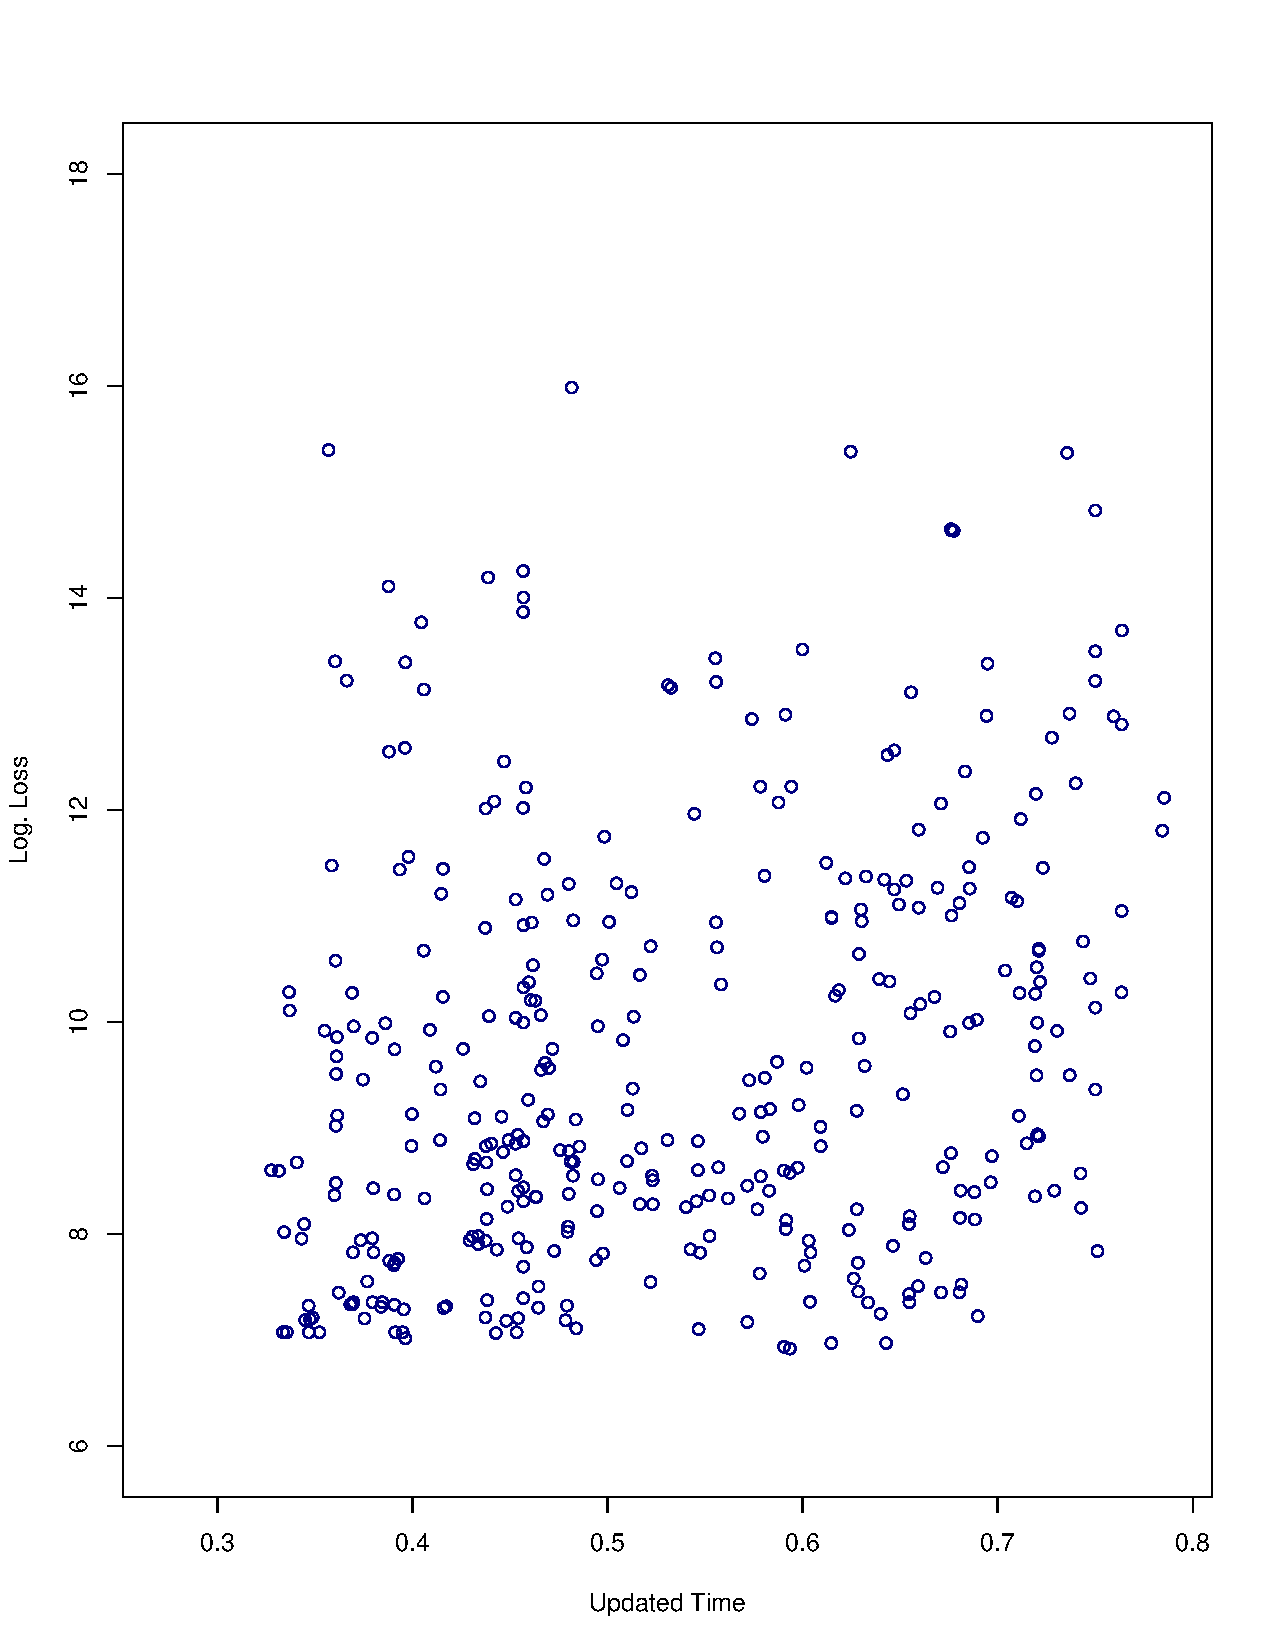
\includegraphics[height=5.5cm, width=7.5cm]{IntraDayUpdatedTime.pdf}
         &
         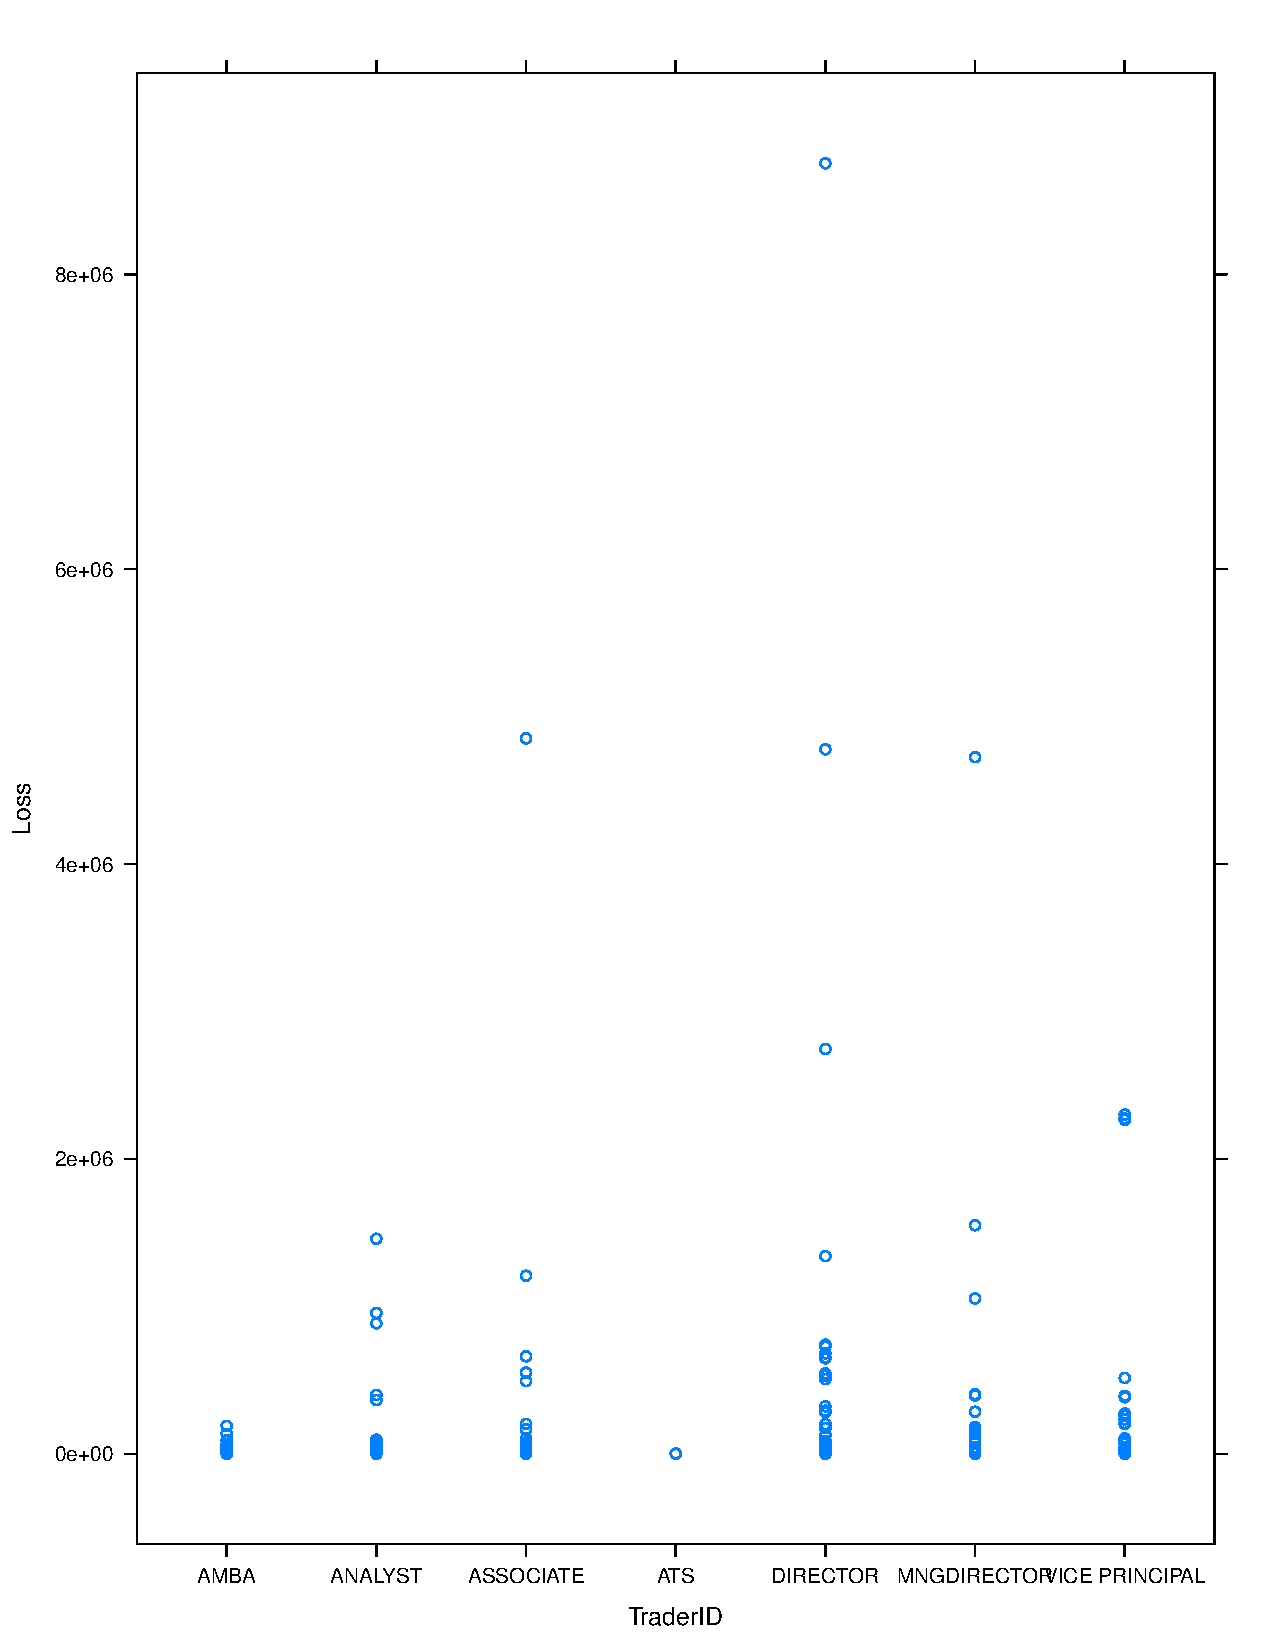
\includegraphics[height=5.0cm, width=7cm]{TrendTraderId.pdf}
         \end{tabular}
    \end{frame}
\subcaption{Intra-day trend analysis of loss severities: overall and as per trading role}
   \label{Intra_Day_Trends} 
\end{subfigure}

\begin{subfigure}[b]{0.55\textwidth}
   \begin{frame}
      \centering
       \begin{tabular}{cc}
        OpRisk events during month & Trading frequency \\
        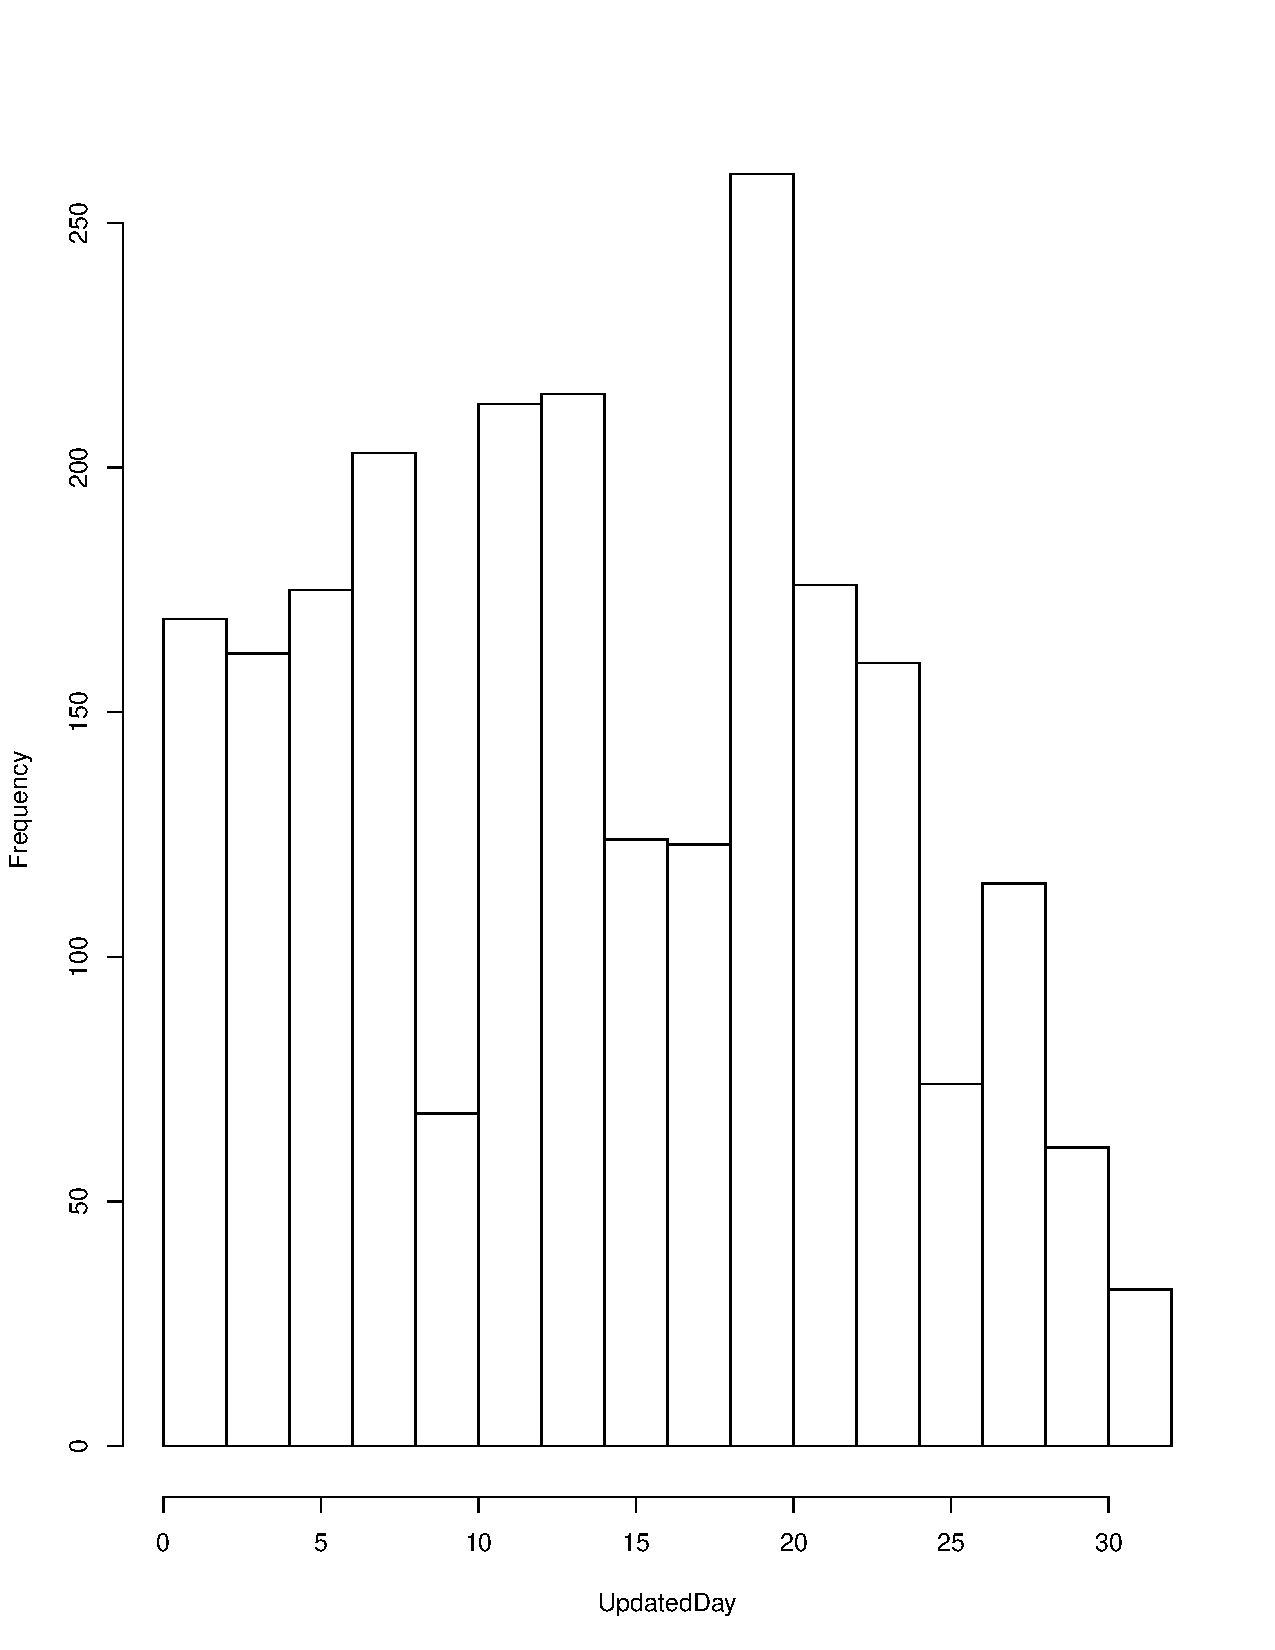
\includegraphics[height=5.5cm, width=7.5cm]{UpdatedDayFreq.pdf}
         &
         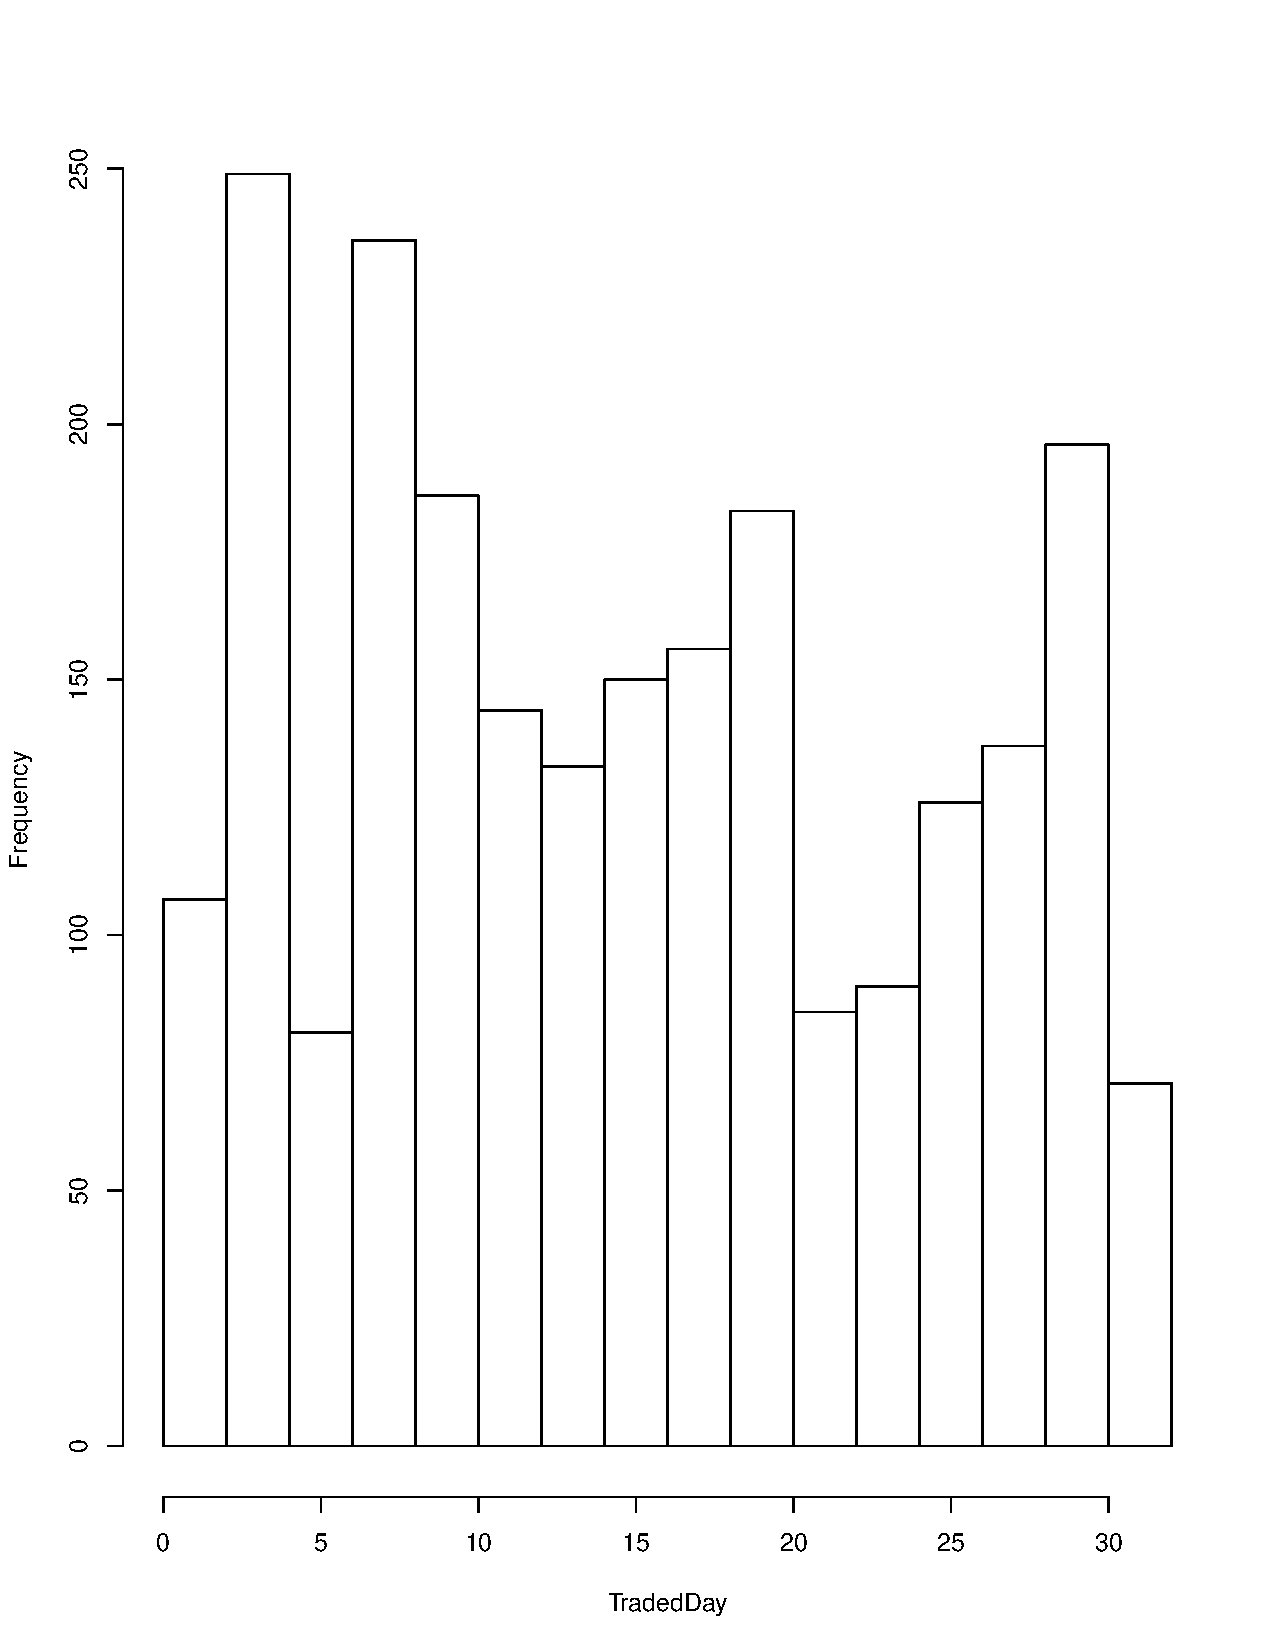
\includegraphics[height=5.5cm, width=7.5cm]{TradedDayFreq.pdf}
         \end{tabular}
    \end{frame}
\subcaption{Intra-month trends of OpRisk trading incidents compared to frequency of trading activity}
   \label{Hist_Loss_Freq}
\end{subfigure}
\caption[Numerical grid display]{(a) Scatterplots of intra-day trend analysis for logs of severities of operational events and for those identifying the trading role responsible/originating the loss incidents. (b) As for (a) but intra-month, and in the form of histograms depicting the frequency distrbution of the number daily operational indicents and the frequency of trades.} 
\end{figure}

\subsection{Characteristics of exposure}

The exposure of risk of type \(i\), \(d_i\) shows the daily duration,
from when the trade was booked to the moment the operational risk event
was observed and ended. This measure is defined this way when
specifically applied to projecting the number of loss events
(frequencies) and can be plotted as follows depicted in graphs depicted
in Figure \ref{Exploration_analysis_exposure}.\medskip

\begin{figure}
\begin{frame}
      \centering
       \begin{tabular}{ccc}
        Distribution & Density & Digital Analysis \\
        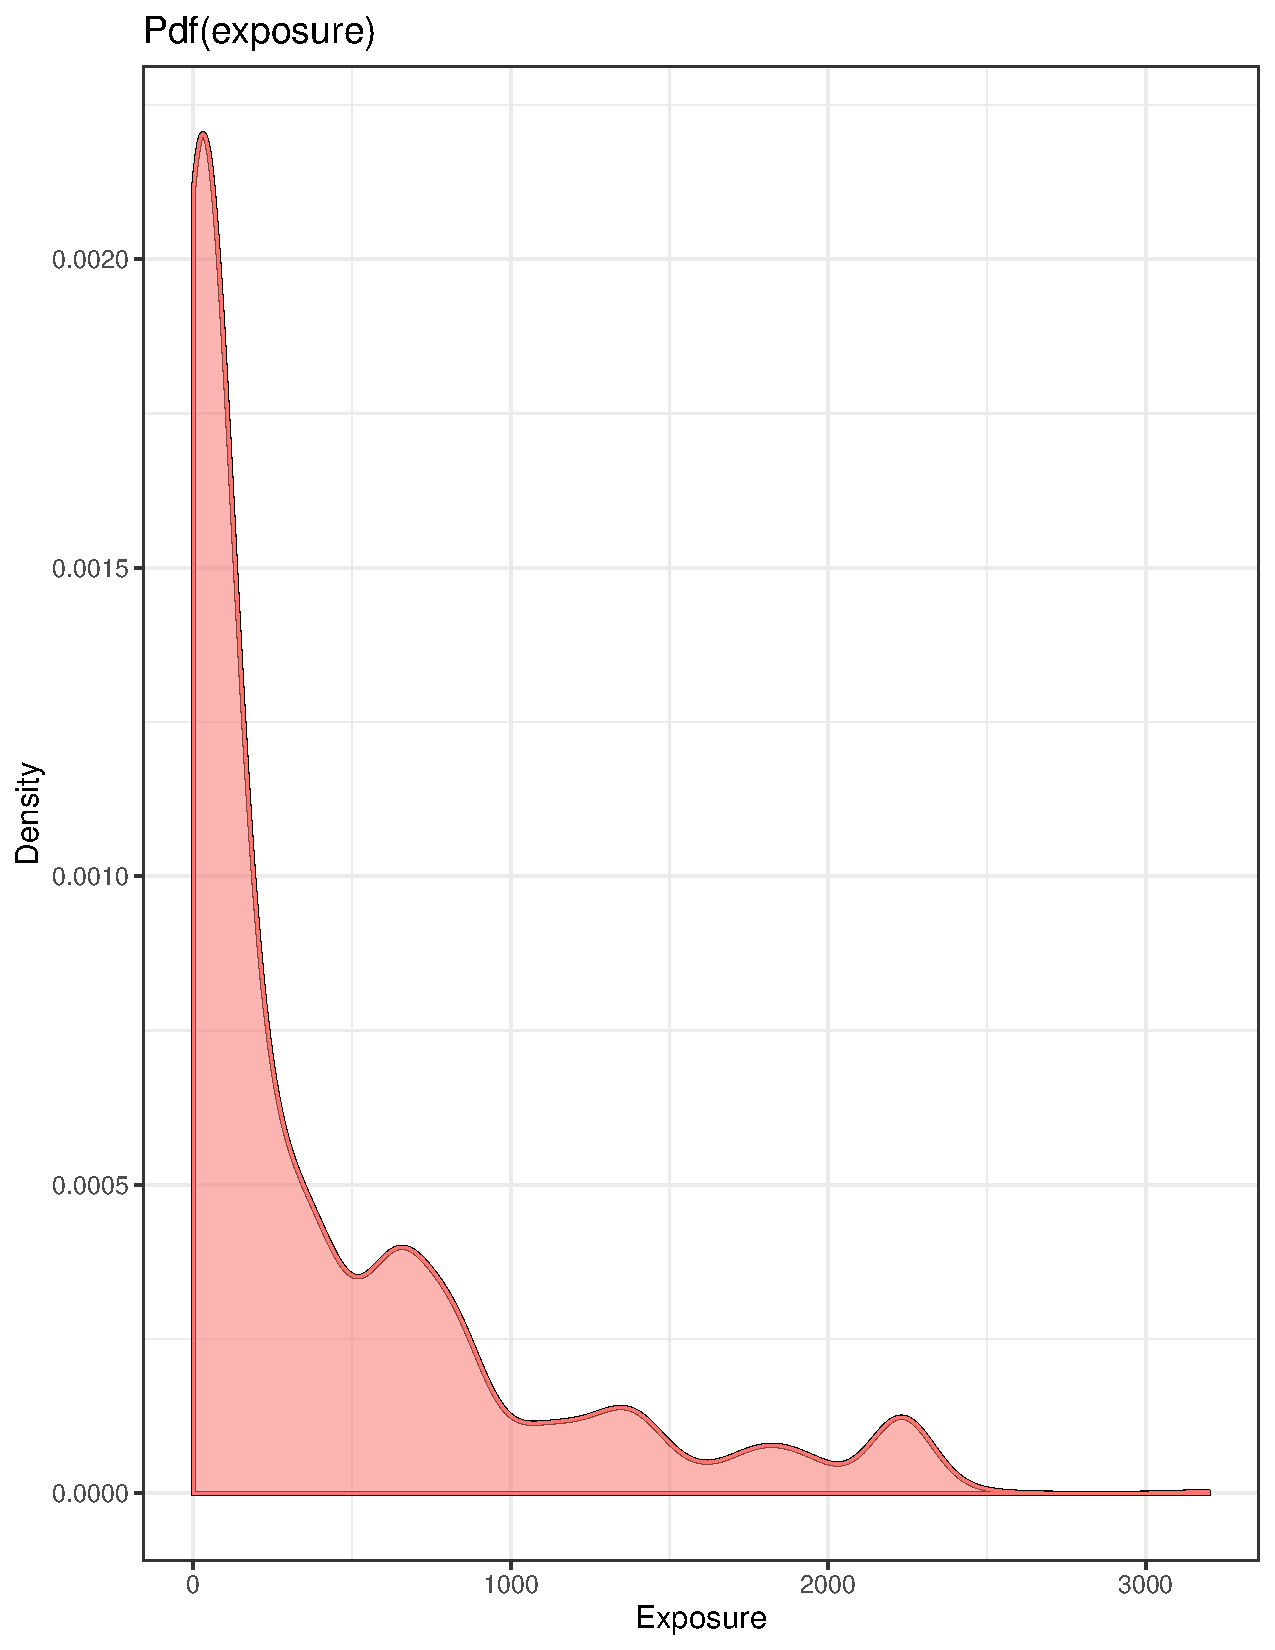
\includegraphics[height=7.5cm, width=5cm]{Exposure_cdf.pdf}
         &
         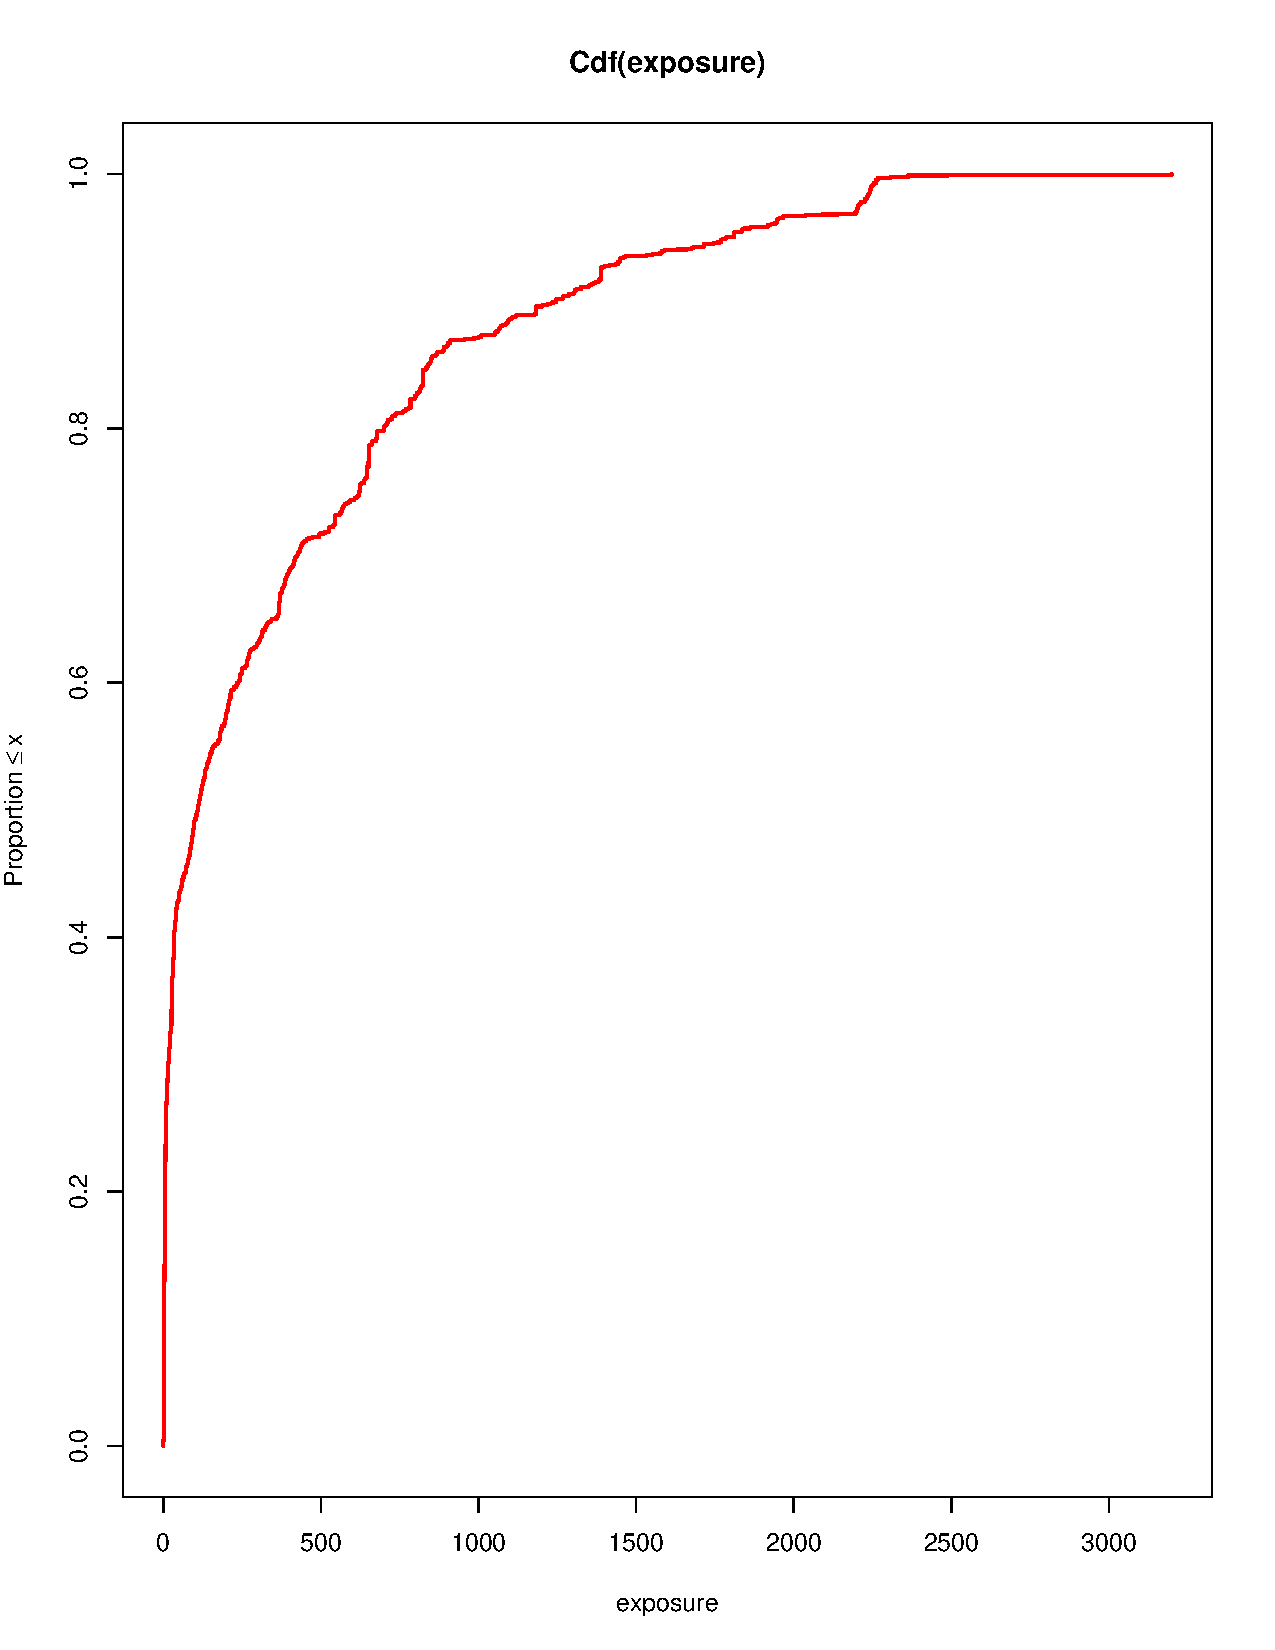
\includegraphics[height=7.5cm, width=5cm]{Dist_exposure.pdf}
         &
         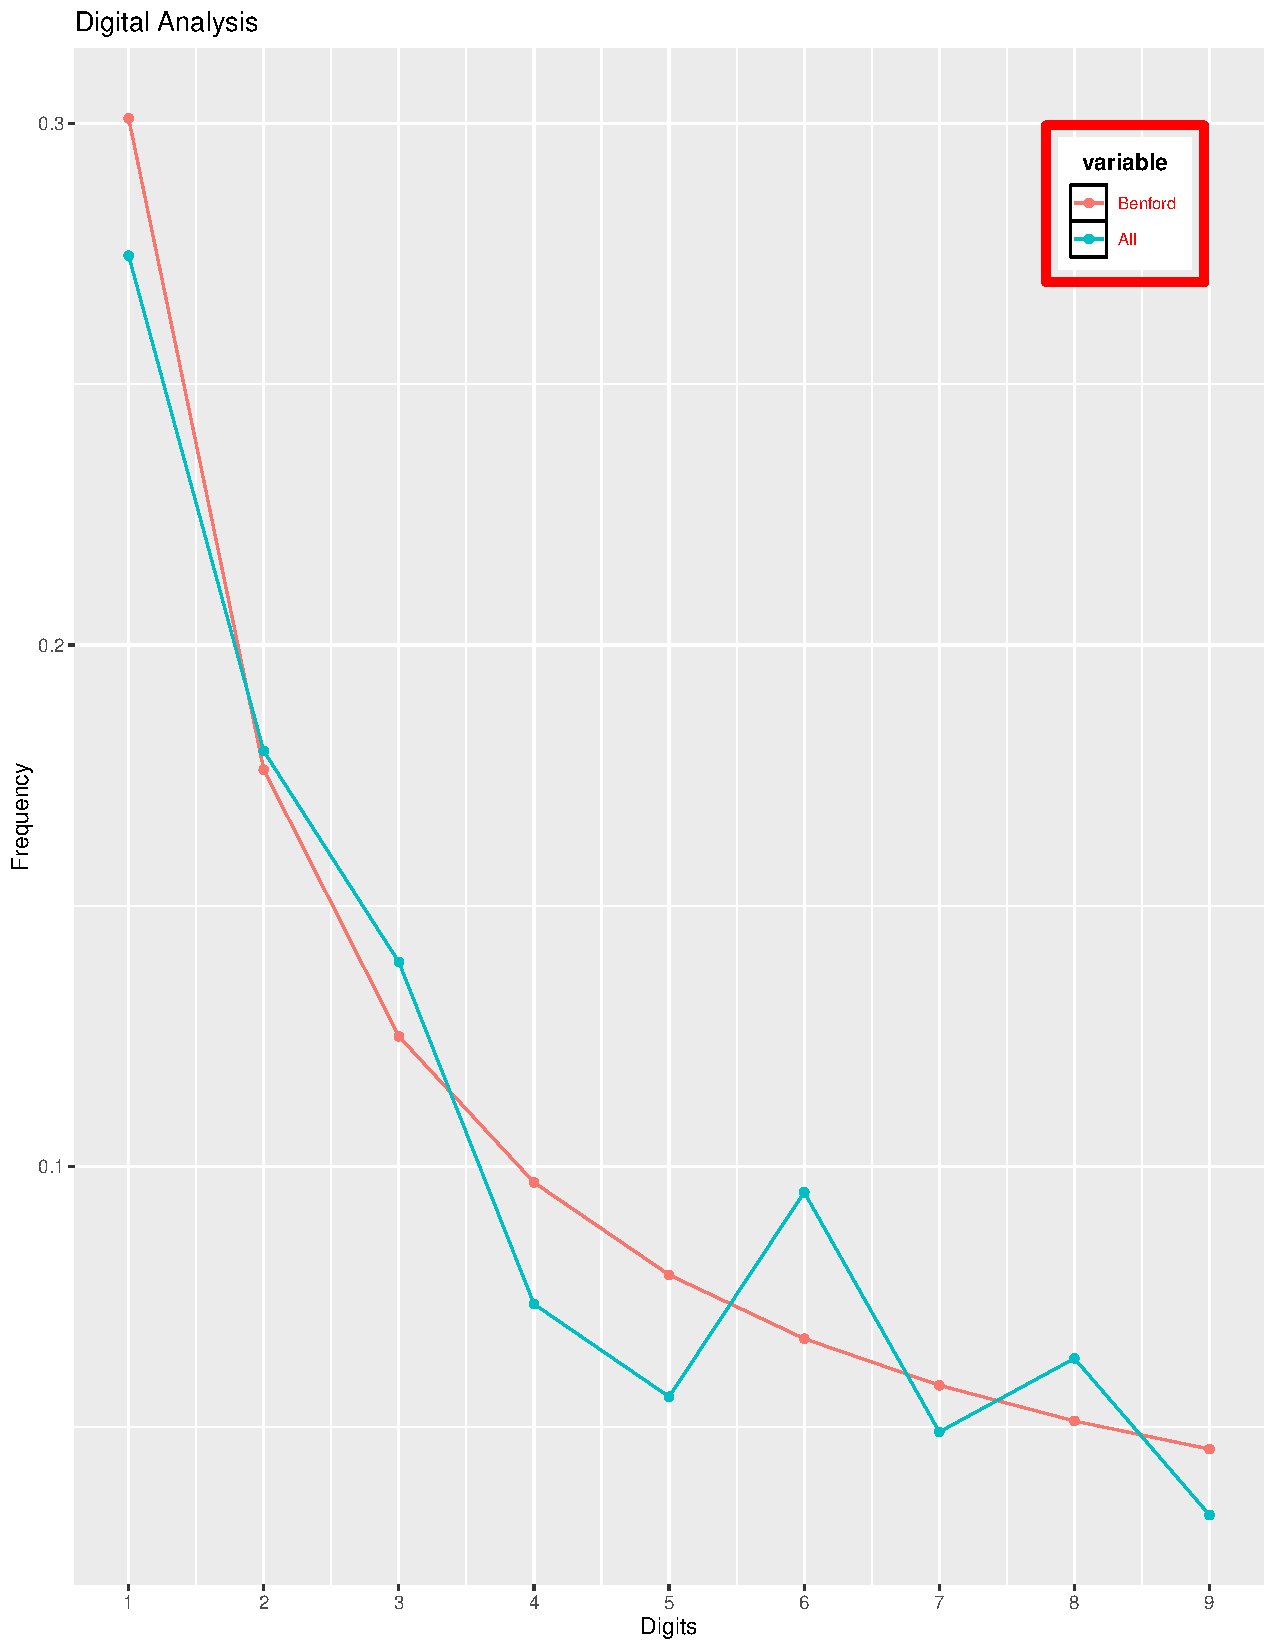
\includegraphics[height=7.5cm, width=5cm]{Benford.pdf}
         \end{tabular}
    \end{frame}
        \captionof{figure}{A simple comparison of the Sigmoidal like features of the fat-tailed, right skewed distribution for the Exposure variable, and first-digit analysis of frequency distribution from the exposure data with the expected distribution according to Benford's Law}
    \label{Exploration_analysis_exposure}
\end{figure}

The variable follows a logistic trend on \([0,1]\), implying an FIs
operational risk portfolio rises like a sigmoid function throughout the
period of observation, typically starting from \(0\), which then
observes a plateau in growth. The average exposure is 389.99 or about 1
year.\medskip

Grid plots \ref{Exploration_analysis_exposure} portray the logistic
function, together with a simple comparison of first-digit frequency
distribution analysis, according to Benford's Law, with exposure data
distribution. The close fitting nature implies the data are uniformly
distributed across several orders of magnitude, especially within the 1
year period.\medskip

\subsection{Characteristics of the covariates}

The characteristics of the operational risk portfolio are given by the
following covariates: \emph{UpdatedDay}, \emph{UpdatedTime} - the day of
the month and time of day the OpRisk incident occurs respectively;
\emph{TradedDay}, \emph{TradedTime} - the day in the month and time of
day the deal was originated respectively; The \emph{LossIndicator} as
indicated before is a binary variable consisting of two values: A \(0\),
which indicates pending or near misses, and \(1\), if the incident
results in a realised loss, meaning that there is significant p\&L
impact due to the OpRisk incident.\medskip

the \emph{Desk} is the location in the portfolio tree the incident
originated, it is a factor variable conisting of 10 categories;
\emph{CapturedBy}, the designated analyst who actions the incident, a
factor variable consisting of 5 categories; \emph{TraderId}, the trader
who originates the deal, a factor variable with 7 categories;
\emph{TradeStatus}, the live status of the deal, a factor variable with
4 categories; \emph{Instrument}, the type of deal, a factor variable
with 23 categories; \emph{Reason}, a description of the cause of the
OpRisk incident, a factor variable with 19 levels;
\emph{EventTypeCategoryLevel}, 7 OpRisk event types as per Risk (2001),
a factor variable with 5 categories; \emph{BusinessLineLevel}, 8 OpRisk
business lines as per Risk (2001), a factor variable with 8
categories.\medskip

\singlespacing

\doublespacing

The continuous numerical variable \emph{Loss}, shows the financial
impact (severity) of the OpRisk incident in Rands. For the most part
(i.e.~96.1\% of the time) OpRisk incidents result in pending losses
and/or near misses, most realised losses (2.3\%) lie within the
{[}\textbf{R$200,00$}, \textbf{R$300,000$}{]} range. In the current
portfolio there are also five p\&L impacts higher than
\textbf{R$2.5$ million}.\medskip

\subsection{Characteristics of daily operational activity}

The distribution of daily losses and/or pending/near misses by
operational activities are represented in
\ref{Exploratory_Time_Day_Frequency3plot}. Figure
\ref{Exploratory_UpdateTime_Frequency3plot} shows that most operational
events occur in times leading up to midday (i.e.~10:50AM to 11:50AM),
the observed median is 11:39AM, and of these potential loss events, most
realised losses occur closest to mid-day. The frequencies of the loss
incidents in the analysed portfolio sharply decreases during the
following period, i.e.~from 12:10PM to 13:10PM, during which the least
realised losses occur.\medskip

Figure \ref{Exploratory_UpdateDay_Frequency3plot} shows that operational
activity increases in intensity in the days leading up to the middle of
the month, i.e.~\(10^{th}\) - \(15^{th}\); the observed mean is
\(14.49\) days, and of these potential loss events, realised losses
especially impact on the portfolio during these days.

\singlespacing

\doublespacing

\begin{figure}
\centering
\begin{subfigure}[b]{0.5\textwidth}
   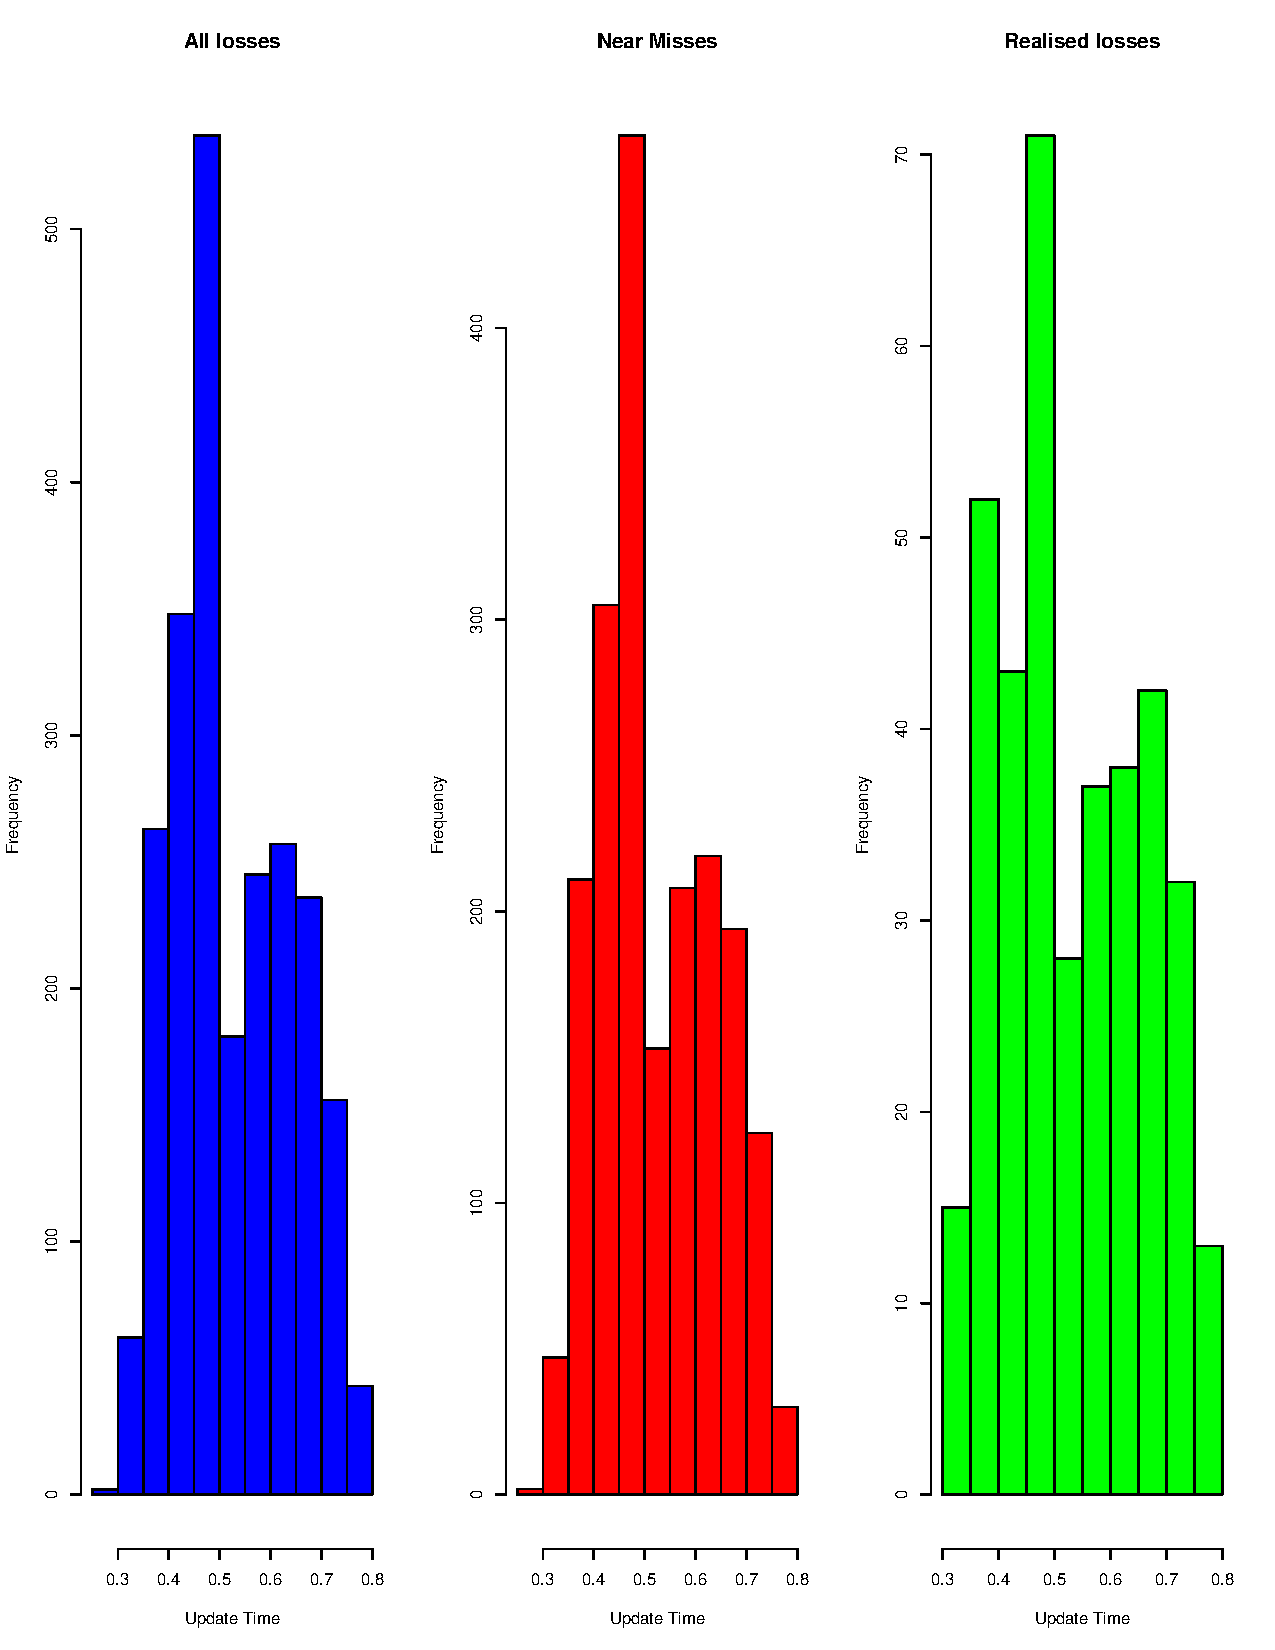
\includegraphics[width=\linewidth]{Exploratory_UpdateTime_Frequency3plot.pdf}
   \subcaption{Incidents by the time in the day}
   \label{Exploratory_UpdateTime_Frequency3plot} 
\end{subfigure}

\begin{subfigure}[b]{0.5\textwidth}
   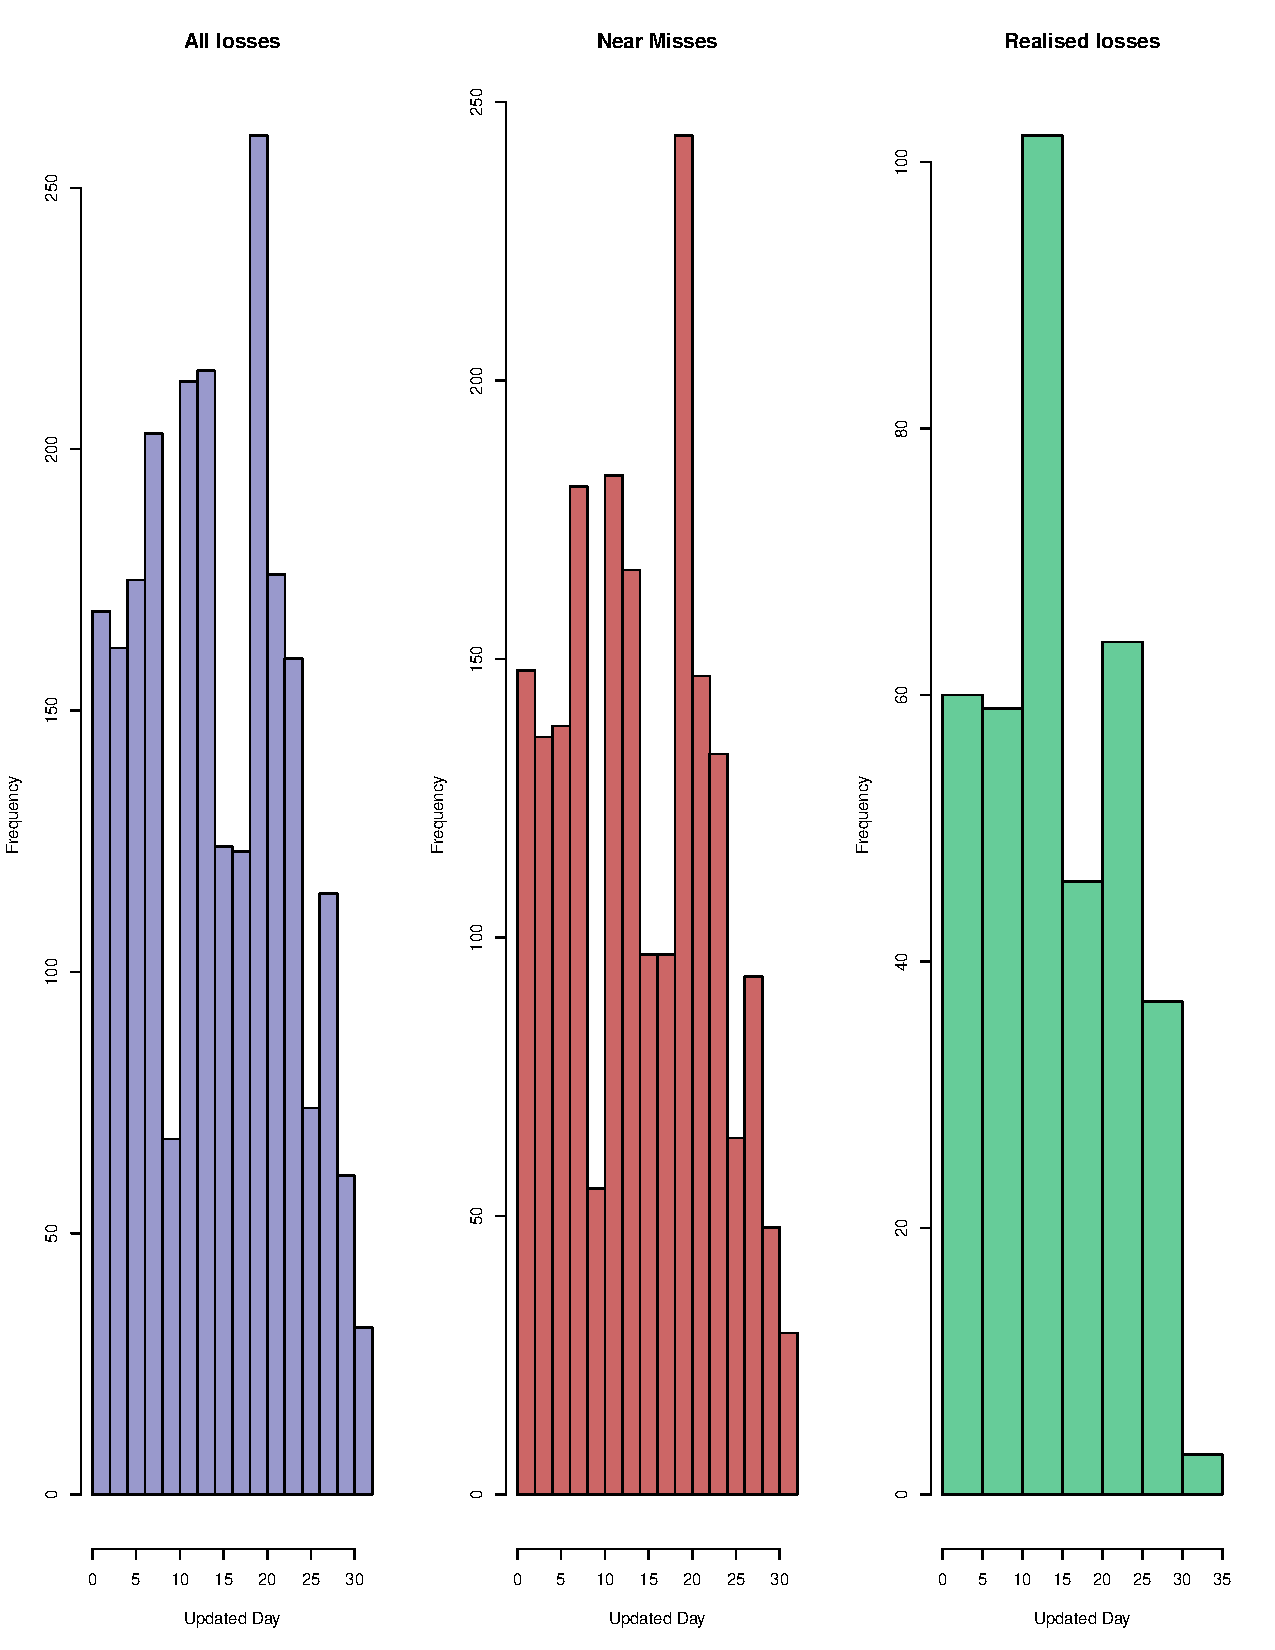
\includegraphics[width=\linewidth]{Exploratory_UpdateDay_Frequency3plot.pdf}
   \subcaption{Incidents by the day in the month}
   \label{Exploratory_UpdateDay_Frequency3plot}
\end{subfigure}

\caption[Two numerical solutions: Histograms showing the distribution of UpdatedTime \& UpdatedDay by LossIndicator.]{The frequency distributions of All the losses, the realised losses, and pending/near misses of operational incidents by the day in the month when the indidents' occurred}
\label{Exploratory_Time_Day_Frequency3plot}
\end{figure}

Similarly, the influence of trading desk's on the frequency of
operational events can be analysed on the basis of the portfolio's
bidimensional distribution by variables \emph{Desk} and
\emph{LossIndicator}, which shows the proportions realised losses vs
pending and/or near misses for each particular desk. The bidimensional
distribution of \emph{Desk} and \emph{LossIndicator} is presented in a
contingency table, Table \ref{tab_Desk_Prop}, in which it's considered
useful to calculate proportions for each desk category.

\begin{figure}
\centering
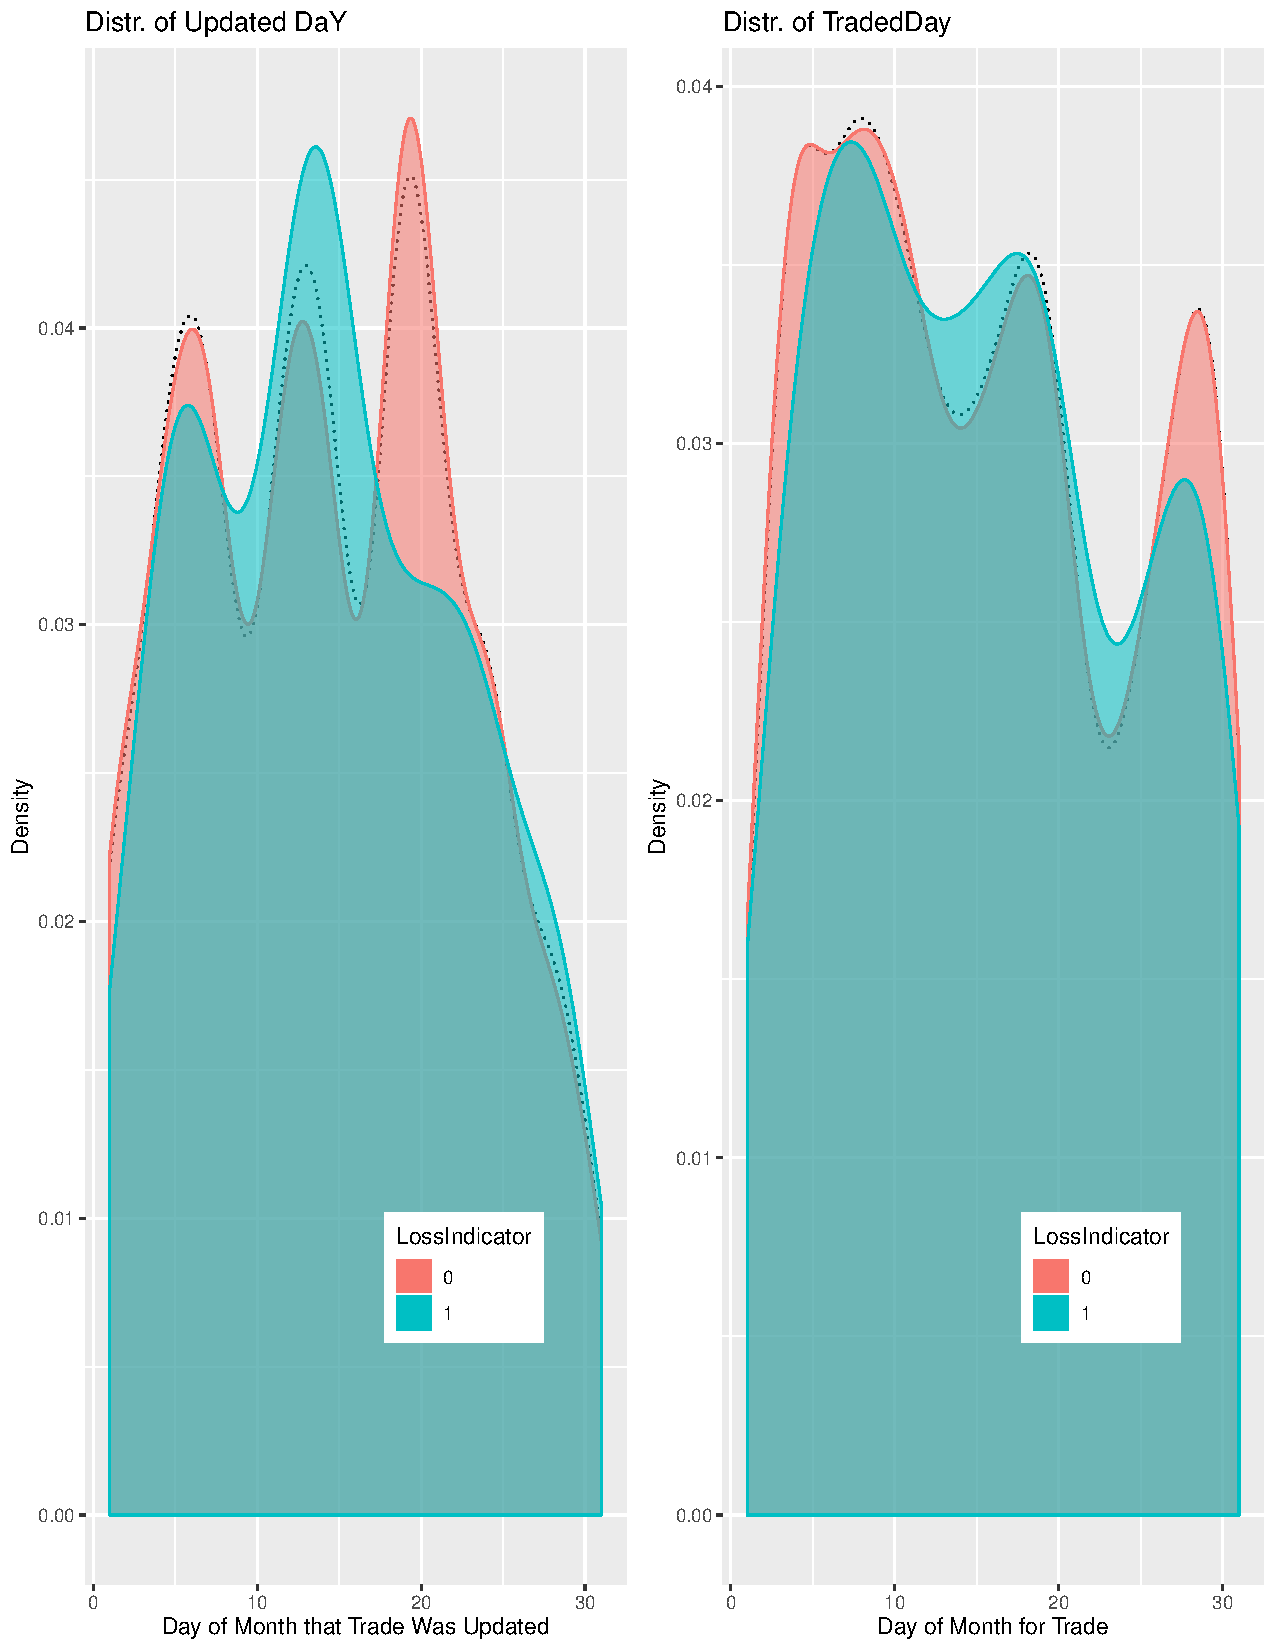
\includegraphics[width=15cm,height=5cm]{Density_UpdateDay_TradedDay.pdf}
\caption[Density plots showing a comparison of realised vs pending losses and/near misses over a month for the day in the month the OpRisk incident was updated to the day in the month trades were traded/booked]{Density plots showing a comparison of realised vs pending losses and/near misses over a month for the day in the month the OpRisk incident was updated to the day in the month trades were traded/booked}
\label{Density_Proportions}
\end{figure}

\singlespacing

\doublespacing

\begin{table}[ht]
\centering
\caption{Occurence of realised losses: proportions on desk categories}
\begin{tabular}{lccr}
\toprule
  & \multicolumn{3}{c}{No. of transactions} \\
Desk   & no Loss   & Loss & Total\\ 
\midrule
  Africa            &  49 & 10 &  59 \\
  Bonds/Repos       & 113 & 31 & 144 \\
  Commodities       & 282 & 45 & 327 \\
  Derivatives       & 205 & 24 & 229 \\
  Equity            & 269 & 66 & 335 \\
  Management/Other  &  41 &  2 &  43 \\
  Money Market      & 169 & 52 & 221 \\
  Prime Services    & 220 & 62 & 282 \\
  Rates             & 336 & 53 & 389 \\
  Structured Notes  & 275 & 26 & 301 \\
 \bottomrule
\end{tabular}\label{tab_Desk_Prop}
\end{table}

Thus, as illustratred in figure \ref{Desk_Proportions}, from 23,5\%; the
highest proportion of realised losses per desk is the Money Market (MM)
desk, the figures are decreasing, followed by Prime Services (22\%);
Bonds/Repos (21,5\%); Equity (19,7\%); Africa (16,9\%); Commodities
(13,8\%); Rates (13,6\%); Derivatives (10,5\%); Structured Notes (SND)
(8.6\%), to the least proportion in the Management/Other, a category
where only 4,7\% of operations activities were realised as losses.

\singlespacing

\doublespacing

\begin{figure}
\centering
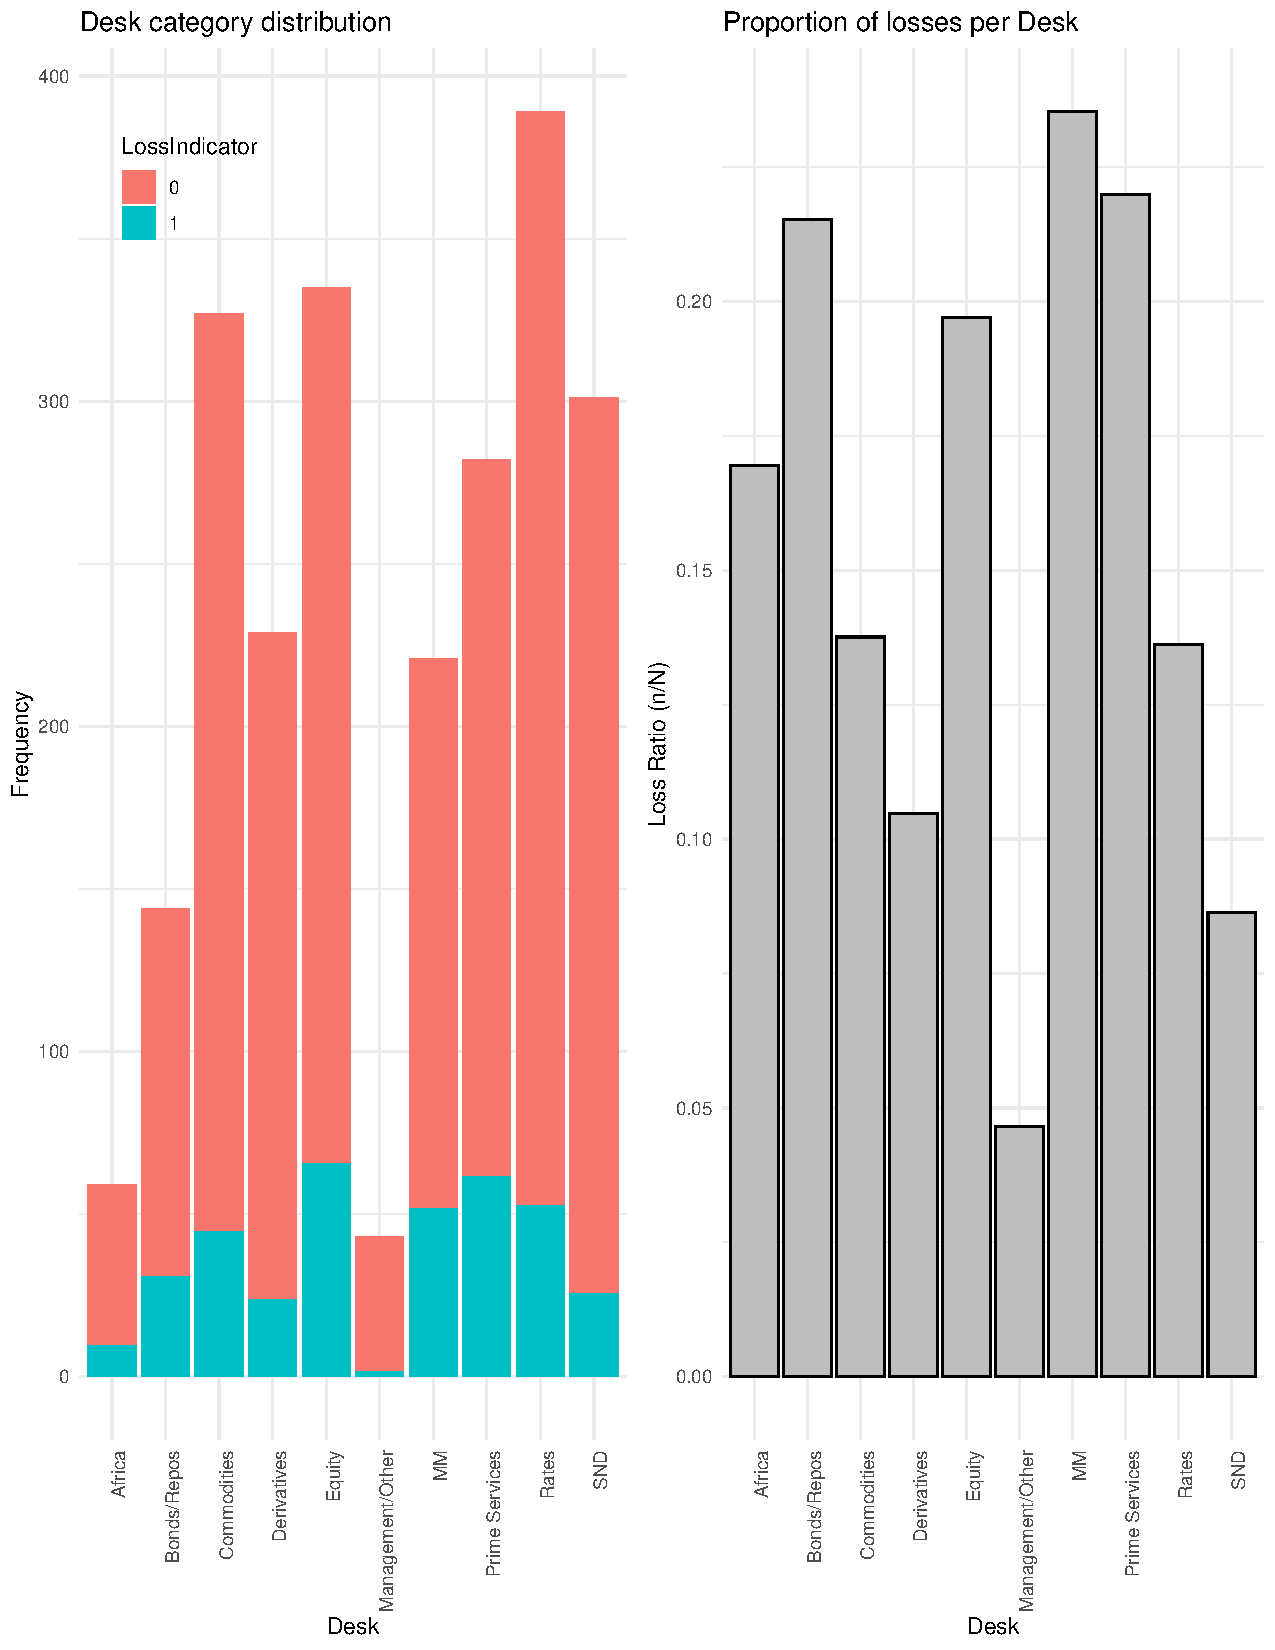
\includegraphics[scale=0.5]{Exploratory_Desk_Proportions.pdf}
\caption[Desk category by realised losses]{Histograms showing the proportions of realised losses vs all losses including pending and/or near misses by desk category}
\label{Desk_Proportions}
\end{figure}

This behaviour can be extended beyond the trading desk, as represented
in Figure \ref{Mosaic_Instr_Trd_Tec}, a mosaic plot grid presenting the
structure of the OpRisk portfolio by Instrument, TraderId, CapturedBy
\footnote{i.e. the type of financial instrument, the trader who originated the incident on the deal, and the role of the technical support personnel who is involved in the query resolution.}
and the operational losses.

\singlespacing

\doublespacing

\begin{figure}
\begin{frame}
      \centering
       \begin{tabular}{cc}
        Type of instrument traded & Role identification \\
        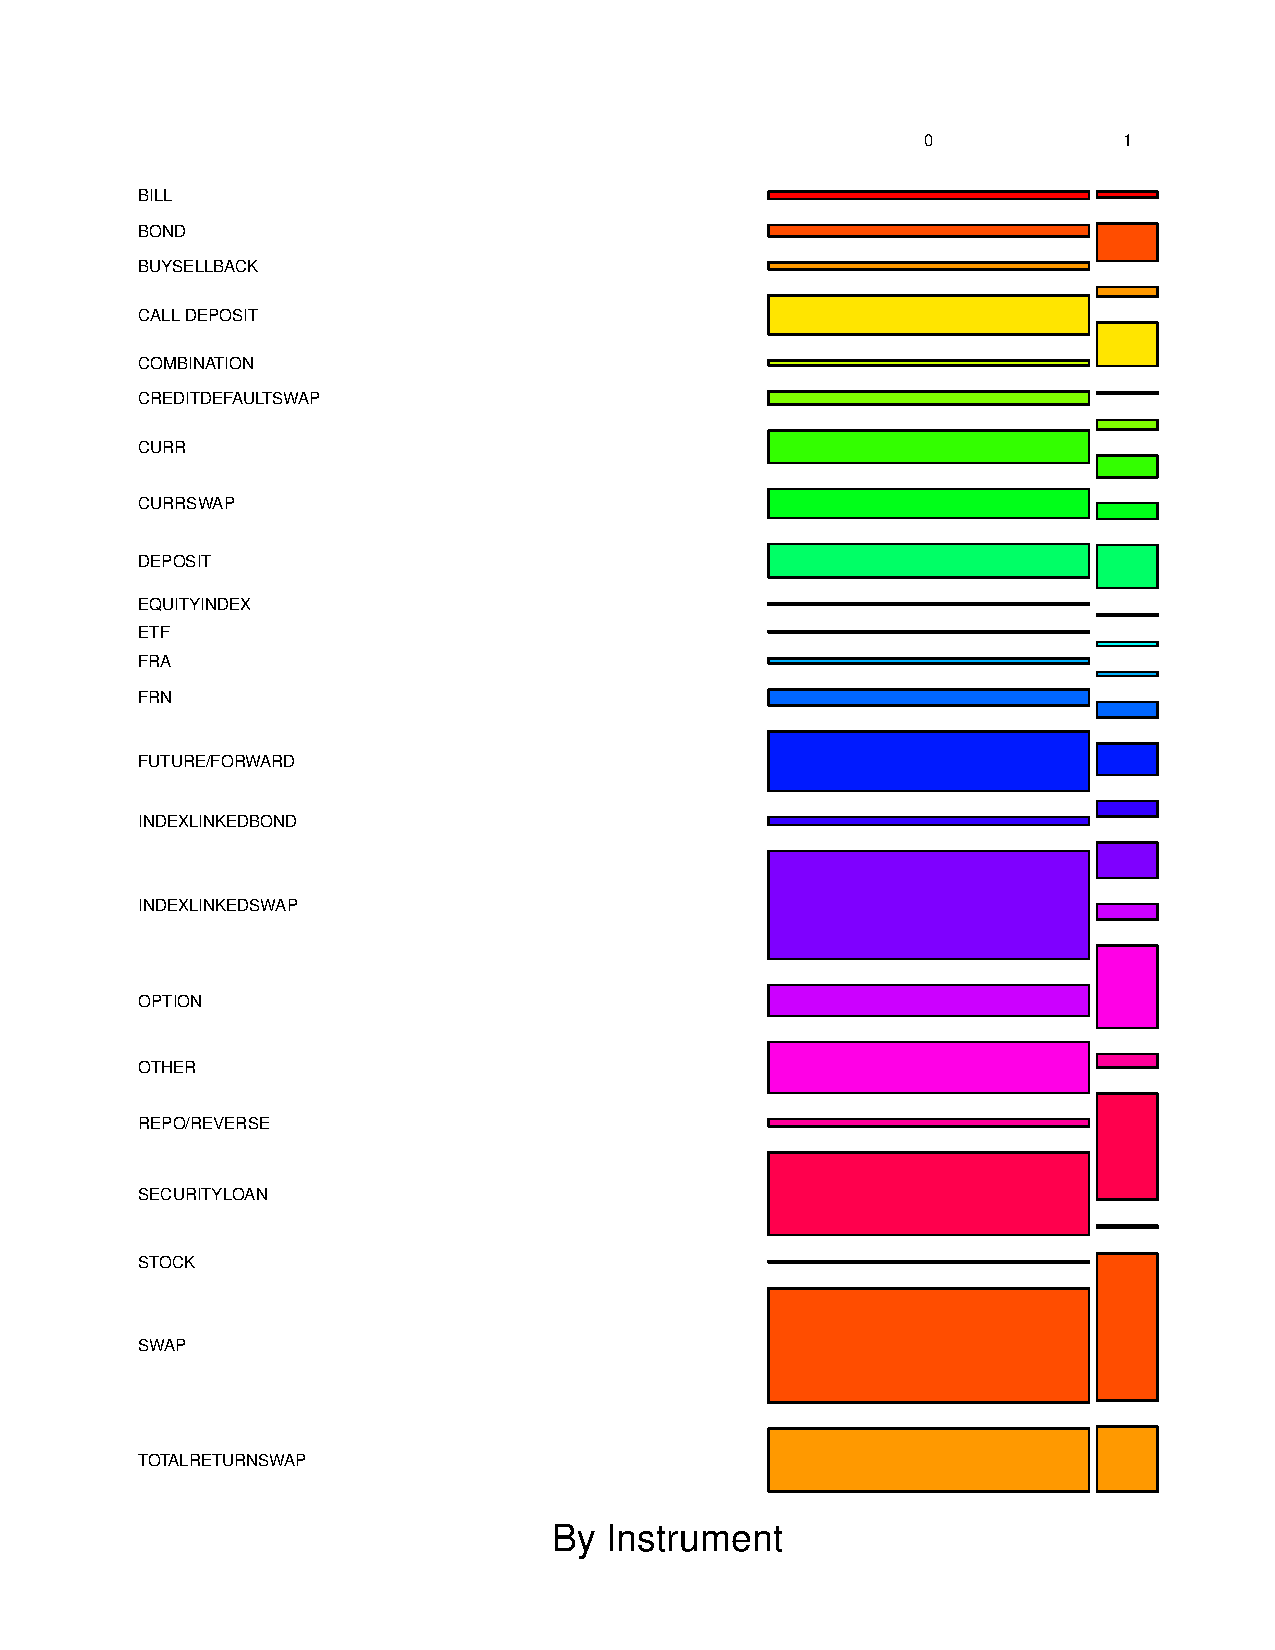
\includegraphics[width=7.5cm,height=18cm]{Single_Instr.pdf}
         &
         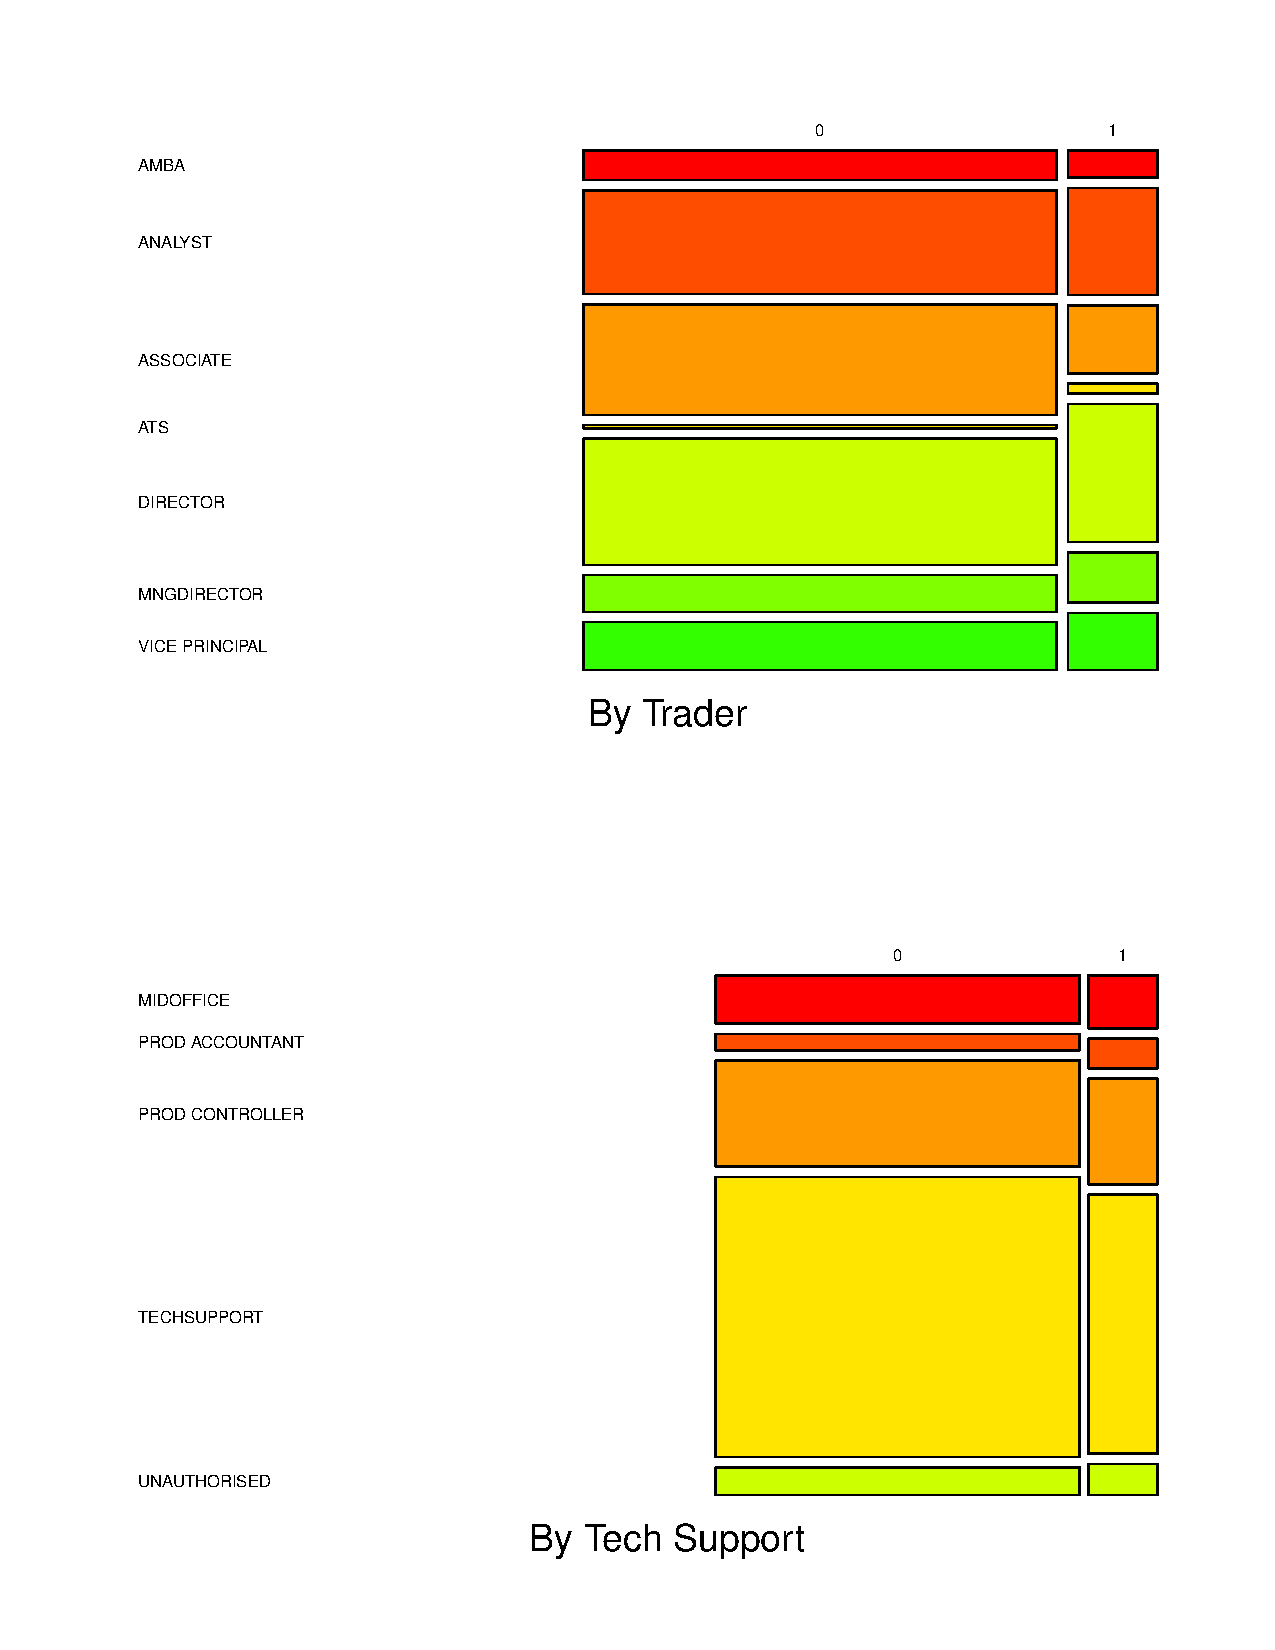
\includegraphics[width=7.5cm,height=18cm]{Stacked_TrId_TechSup.pdf}
         \end{tabular}
    \end{frame}
    \caption{Mosaic grid plots for the bidimensional distribution by traded instrument, the trader originating the operational event, and by the technical support personnel involved in query resolution, against the target variable \texttt{LossIndicator} showing realised losses vs near misses/pending losses reported.}
    \label{Mosaic_Instr_Trd_Tec}
\end{figure}

One can notice that the width of the bars corresponding to the different
categories, i.e.~Instrument, TraderId, CapturedBy, is given by their
proportion in the sample. In particular, for the category `at least one
realised loss', in the top right mosaic of Figure
\ref{Mosaic_Instr_Trd_Tec} portrays a increase in ``riskiness'' trending
up from Associate to AMBA, Analyst, Vice Principal, Managing Director,
Director, up to the risky ATS category, which are automated trading
system generated trades.\medskip

Figure \ref{Mosaic_Instr_Trd_Tec} bottom right mosaic plot for technical
support personnel for the category `at least one realised loss',
portrays a downward trend, slowing in riskiness from Unauthorised User
downward to Tech Support, Mid Office, Prod Controller down to the least
risky Prod Accountant. This intepretation makes sense given unauthorised
users are more likely to make impactful operational errors, technical
support personnel would also be accountable for large impacts albiet for
contrasting reasons, they are mandated to perform these deal adjustments
which have unavoidable impacts associated with them, whereas the former
group are unauthorised to perform adjustments therefore may lack the
skill, or be criminally minded insiders acting on their own or in unison
to enable their underhanded practices and intentions without raising any
suspicion.\medskip   

\begin{table}[!htbp] \centering 
  \caption{Summary statistics for all losses as per Instrument type} 
  \label{Stargazer} 
\begin{tabular}{@{\extracolsep{5pt}}lccccccc} 
\\[-1.8ex]\hline 
\hline \\[-1.8ex] 
Statistic & \multicolumn{1}{c}{N} & \multicolumn{1}{c}{Mean} & \multicolumn{1}{c}{St. Dev.} & \multicolumn{1}{c}{Min} & \multicolumn{1}{c}{Pctl(25)} & \multicolumn{1}{c}{Pctl(75)} & \multicolumn{1}{c}{Max} \\ 
\hline \\[-1.8ex] 
Mean & 23 & 34,603 & 46,007 & 306 & 7,697 & 44,157 & 192,513 \\ 
\hline \\[-1.8ex] 
\end{tabular} 
\end{table}

In another mosaic plot, Figure \ref{Mosaic_Contingency}, the
bidimensional distribution of transactions by trader and realised vs
pending losses, conditional on the trade status is presented and
analysed. Here, and in the contingency table, Table
\ref{tab:Mosaic_Contingency}, we can clearly see the following trends:
In BO-BO confirmed status - an increase in realised losses from the
leftmost TraderID (i.e.~AMBA) to right, and the opposite for
transactions performed in BO Confirmed status (both with two
exceptions). In particular, the biggest number of realised losses in
both BO and BO-BO Confirmed statuses occur due to automated trading
systems (ATS) who also give rise to the exceptions mentioned.\medskip

\singlespacing

\singlespacing
\begin{figure}
\centering
\textbf{Mosasic plot for trader identification and loss indicator, by trade status}
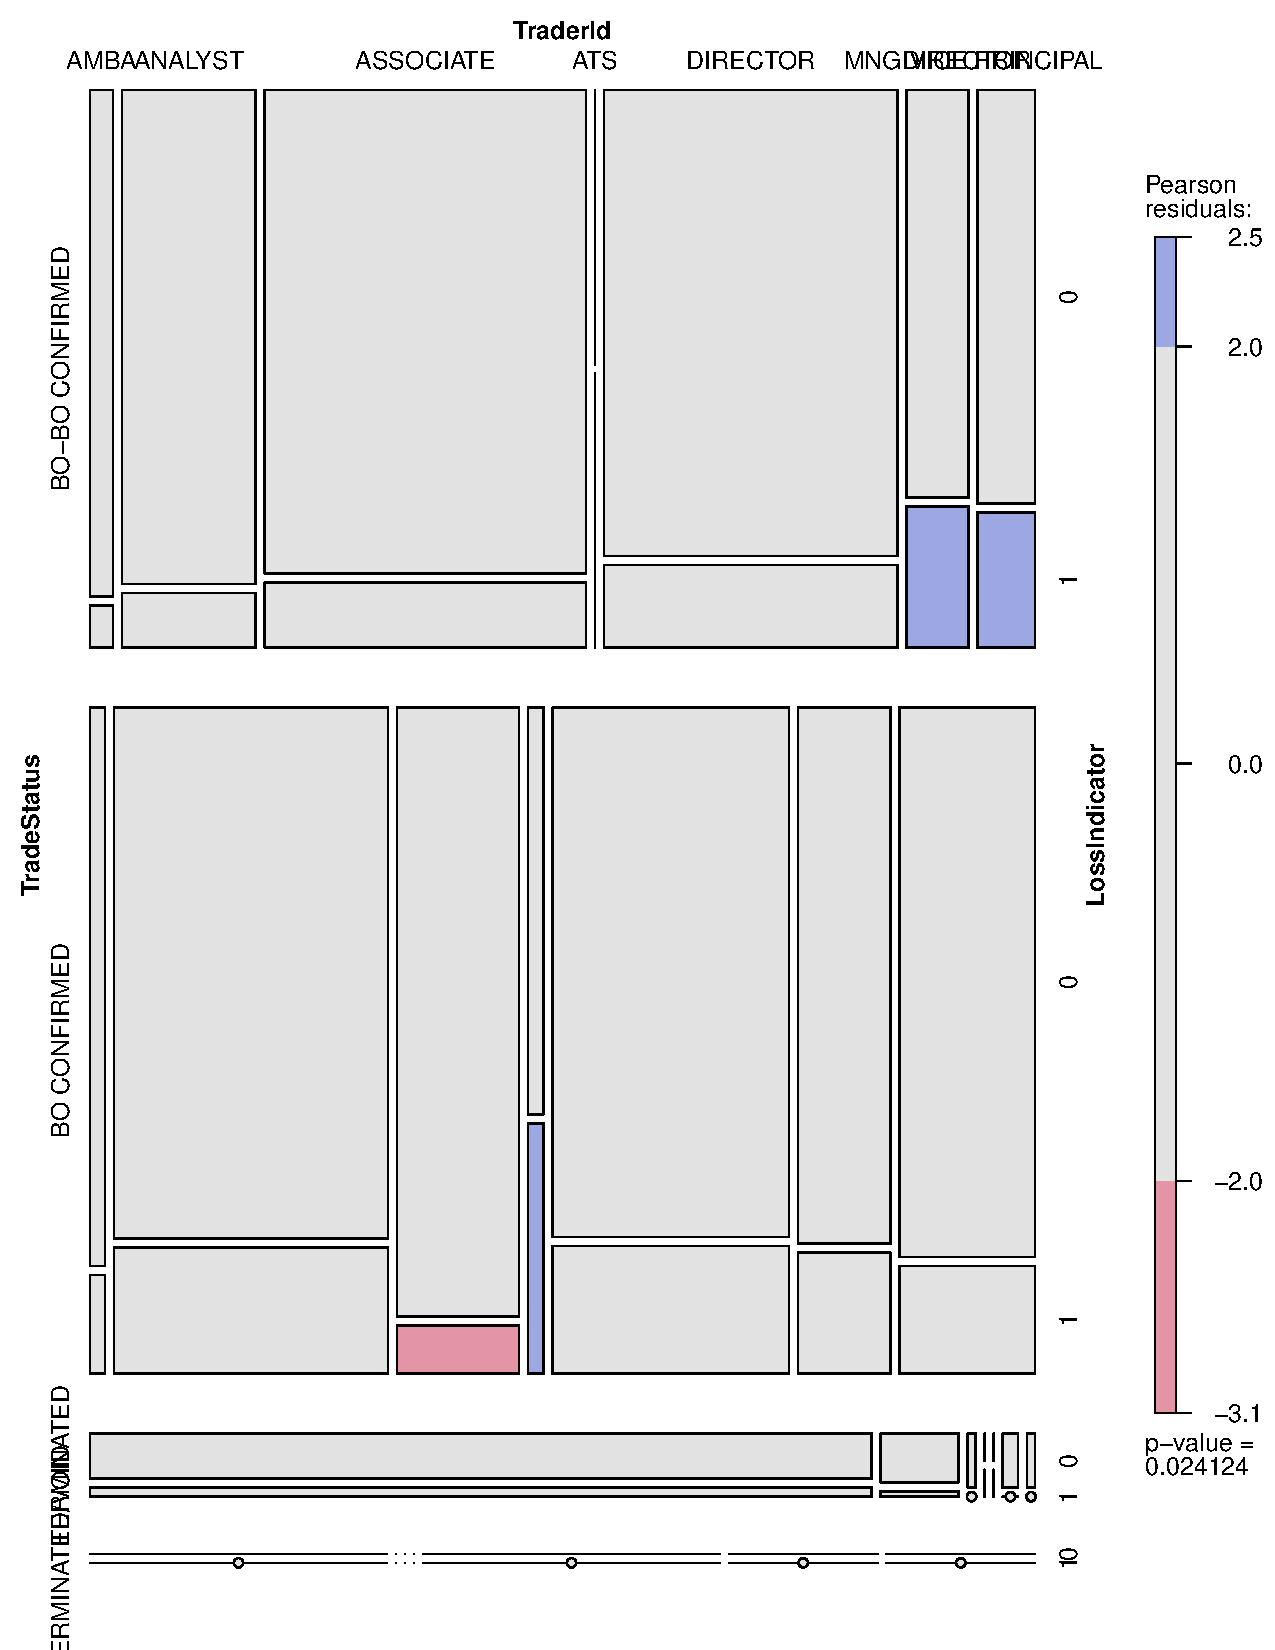
\includegraphics[width=\linewidth,height=0.75\linewidth]{Mosaic_Contingency.pdf}
\caption[Portfolio structure by trader, trade status and number of realised losses]{A mosaic plot representing the structure of the operational risk portfolio by trader identification (TraderId), the status ofthe trade (TradeStatus) and the number of realised losses vs pending or near misses}
\label{Mosaic_Contingency}
\end{figure}
\doublespacing

Table \ref{tab:Crosstab_covariate} presents the most frequent category
in the operational risk dataset for each possible covariate.

\begin{table}[htbp]
        \centering
        \textbf{Crosstab of trader identification and loss indicator, by trade status}
\singlespacing        
        \small
        \setlength\tabcolsep{2pt}
            \begin{tabular}{|p{3cm}|p{2cm}|l|l|l|l|l|l|p{2cm}|p{2cm}|} \hline
            & & \multicolumn{7}{|c|}{Trader Identification} \\ \hline
            TradeStatus & Loss Indicator & Amba & Analyst & Associate & ATS & Director & Mng Director & Vice Principal \\\hline
            \multirow{2}{*}{BO-BO Confirmed} & 0 & 24 & 136 & 320 & 0 & 282 & 52 & 49 \\ \cline{2-9}
                                   & 1 & 2  &  15 & 43 & 0 & 50 & 18 & 16 \\\cline{2-9}
            \multirow{2}{*}{BO Confirmed} & 0 & 17  & 299 & 153 & 13 & 257 & 102 & 153 \\ \cline{2-9}
                                   & 1 &  3 &  71 & 12 & 8 &  62 & 23 & 30 \\ \cline{2-9}
            \multirow{2}{*}{Terminated}       & 0 & 83 & 9 & 1 & 0 & 0 & 2 & 1 \\ \cline{2-9}
                                  & 1 & 17 & 1 & 0 & 0 & 0 & 0 & 0 \\ \cline{2-9}
            \multirow{2}{*}{Terminated/Void}  & 0 & 2 & 0 & 0 & 0 & 2 & 1 & 1 \\ \cline{2-9}
                                   & 1 & 0 & 0 & 0 & 0 & 0 & 0 & 0 \\ \hline
            \end{tabular}
            \caption{A contingency table showing the bidimensional distribution of transactions by trader identification vs realised and/or pending losses, conditional on the trade status}
            \label{tab:Crosstab_covariate}
\end{table}
\doublespacing

\begin{table}[htbp]
        \centering
        \textbf{Modal classes for the categorical variables} 
\singlespacing        
        \small
        \setlength\tabcolsep{2pt}
            \begin{tabular}{|l|l|p{6cm}|} \hline
            Variable & Modal class or category & Name of modal class \\\hline
            Desk & Rates & DeskRates \\ \cline{1-3}
            CapturedBy & TECHSUPPORT & CapturedBy\_TECHSUPPORT \\ \cline{1-3}
            TradeStatus & BO confirmed & TradeStatus\_BO confirmed \\ \cline{1-3}
            TraderId & DIRECTOR & TraderId\_DIRECTOR \\ \cline{1-3}
            Instrument & Swap & Instrument\_Swap \\ \cline{1-3}
            Reason & Trade enrichment for system flow  & Reason\_Trade enrichment for system flow \\ \cline{1-3}
            EventTypeCategoryLevel & EL7 & EventTypeCategoryLevel\_EL7 \\ \cline{1-3}
            BusinessLineLevel & BL2 & BusinessLineLevel\_BL2 \\ \cline{1-3} 
            \end{tabular}
            \caption{A contingency table showing the bidimensional distribution of transactions by trader identification vs realised and/or pending losses, conditional on the trade status}
            \label{tab:Mosaic_Contingency}
\end{table}
\doublespacing

\singlespacing

\FloatBarrier
\newpage
\fancyhead[L]{Exposure-based Operational Risk Analysis}
\fancyhead[R]{\thepage}
\fancyfoot[C]{}

\chapter{EXPOSURE-BASED OPERATIONAL RISK ANALYSIS}
\label{EXPOSURE-BASED OPERATIONAL RISK ANALYSIS}

\doublespacing

\section{Introduction}
\label{sec3:Introduction}

The fundamental premise behind the nature of ORMF's is to provide an
exposure-based treatment of OpRisk losses which caters to modeling
capital estimates for forward-looking aspects of ORM. This proves tricky
due to the need for specific knowledge about potential loss events
viz.~the required knowledge of the likelihood and magnitude of a loss
from the time the loss event occurs until the actual realised loss
materialises, given a case specific underlying loss-generating
mechanism. By this very nature OpRisk is being characterised by the
significant lag that results between the moment the event is conceived
to the point the loss materializes.\medskip 

For example, in the case of rogue trading, there is a frequency exposure
associated with traders \emph{going rogue}, due to a probability of
rogue events happening between a specific group of traders over time,
which is then modeled for each rogue trading event and the impact
(severity based on the size of the position) of the loss when it is
realised (at time of detection). This timing paradox often results in
questionable capital estimates, especially for those near misses,
pending and realised losses that need to be captured in the model.

\section{Applicability of EBOR methodology for capturing forward-looking aspects of ORM}
\label{sec:Applicability of EBOR methodology for capturing forward-looking aspects of ORM}

OpRisk is characterised by a time delay \(\tau\), wherein the p\&l
impact lags behind the moment the OpRisk event is conceived up until the
event is observed and accounted for. In this paper the author advances
knowledge of the current ORMF's toward a new EBOR framework which aims
to provide an exposure-based treatment of OpRisk losses catering for
modeling capital estimates of forward-looking aspects of OpRisk.\medskip

Einemann et al. (2018) unearth the current EBOR model anagolous to the
BL/ET matrix combinations in the LDA model, wherein an additional cell
is considered in the classical LDA model whose contributions build a
hybrid ORMF which integrates EBOR models with the LDA model,
facilitating the migration of OpRisk types from a classical to EBOR
treatment through a quantitative framework (Einemann et al., 2018).
Conceptually, the EBOR model component can be extended to include
potential future events e.g., future litigations, based on some
underlying property, capturing forward looking aspects of business
environment and internal control factors (BEICF's) thereof.\medskip

The fundamental premise behind the LDA is that each firm's OpRisk losses
are a reflection of it's underlying OpRisk exposure (Einemann et al.,
2018). Dobson \& Barnett (2008) relates OpRisk events to a varying or a
constant degree of exposure, which needs to be taken into account when
modeling counts or frequencies of occurance. In particular, the
assumption behind the use of the Poisson distribution in the model to
estimate the frequency of losses for all available observations, is that
both the the intensity (or rate) of occurrence and the opportunity (or
exposure) for counting can assume either of these two afore-mentioned
forms (Dobson \& Barnett, 2008). In the former case the varying degrees
of exposure impact on the rate of events, whereas in the latter case the
exposure is constant hence not relevant to the model.\medskip

When observed counts all have the same exposure, modeling the mean count
\(\mu\) as a function of explanatory variables \(x_{1},\ldots,x_{p}\) is
the same as modeling the rate \(R\). The actual measure of exposure we
need to use depends specifically on projecting the count of OpRisk
events (frequency of realised losses) as the target variable in the
model as opposed to the measure if the target variable were the severity
of the losses, e.g.~in modeling rogue trading severity exposure of
events is based on size of loss position at time to detection or
CapturedBy as severity risk factors.

\section{Sub-problem 1}
\label{sec:Sub-problem 1}

In our prevailing banking phenomena of increasing OpRisks, the problem
consists of questioning whether a firm's susceptibility to OpRisk
hazard's growth, results in the degree of OpRisk losses slowing due to
tightning OpRisk controls and enhancements to OpRisk frameworks. It
would be prudent not to declare things are improving if the evidence is
not quite firm that this is true. This is essentially a check for
situations, from these data, whether there is evidence of the unchecked
spread of negligent behaviour leading to operational loss events or not;
or on the contrary, those situations other than the unrestricted spread
of these ``rogue'' events conscequently driving OpRisk losses i.e.,
which may requiring a re-thinking our approach to improving OpRisk
controls and enhancing OpRisk management frameworks.

\subsection{Exposure-based OpRisk (EBOR) models}
\label{ssec:Exposure-based OpRisk (EBOR) models}

The existing models in OpRisk measurement for which historical loss
distributions are the best predictors of future losses, assume that we
do not learn from past losses. This is problematic for ``predictable''
risk types due to model's practice of undercapitalising known risks
before occur, and overcapitalising for risks after the losses
materialise, creating innappropriate capital estimates (Group \& others,
2013). These concerns motivate the development of an EBOR modelling
framework which not only captures past losses but also how exposures to
forward-looking affect risk attitudes using event frequencies based on
actual exposures in the business environment and internal control risk
factors (BEICF) thereof.

\subsection{Hypothesis 1}
\label{Hyp1:Hypothesis 1}

To quantify OpRisk losses by introducing GLM's, GAMLSS models towards a
new framework for OpRisk management, who are ``predictive'' due to
learning capabilities, capturing exposures to forward-looking aspects in
addition to how past losses affect may risk attitudes. EBOR treatments
effectively replace historical loss severity curves obtained from
historical loss counts, replacing how missed losses are undercapitalized
for, and/or overcapitalizing realised losses after they occur, by
looking for evidence in deep hierarchies of the features from these data
to affirm that this is true.

\section{Derivation of the poisson model from the exponential family of distributions}
\label{sec:Derivation of the poisson model from the exponential family of distributions}

Operational riskiness in FIs grows as trading transactions grow in
complexity i.e., the more complex and numerous trading activity builds
the higher the rate at which new cases of OpRisk events occur.
Therefore, it is likely that the rate of operational hazard may be
increasing exponentially over time. The scientifically interesting
question is whether the data provides any evidence that the increase in
the underlying operational hazard generation is slowing. The
afore-mentioned postulate provides a plausible model to start
investigating this question.\medskip

In the obove discussions, the question of increasing OpRisk hazard rates
due to increasing transaction complexity arises, wherein \(\mu_i\), the
expected number of new cases on day \(t_i\) is modeled. As a starting
point, and with reference to LDA model steps, one begins by using
Poisson modeling for counts to estimate the rate of loss events
frequencies. The Poisson model's flexibility permits the modelling of
numerous operational loss counts and when the data are mostly zeroes and
ones (when Poisson means are low). The model assumes that the number of
expected new OpRisk hazards often increase exponentially over time.
Hence, if \(\mu_i\) is the expected number of new cases over time
\([T,T+\tau] = t_i\), then an appropriate model takes the form:

\singlespacing

\begin{eqnarray}\label{expgrowth}
E(\mathbf{Y}_i) = \mu_i = d_i\exp{(\beta t_i)} 
\end{eqnarray} \doublespacing

where the random variables \(\mathbf{Y_i}\) are independent,
\(d_i = \mbox{exposure}_i\), and \(\beta\)'s are a set of unknown
parameters in \(\mathbf{\beta}\). For a list of \(N\) different Oprisk
events, note that the random variables \(Y_i\) are the basis for the
OpRisk hazard defined by a binary response variable \emph{LossIndicator}
which denotes the presence or absence loss. Define random variabels
\(Y_1,\ldots,Y_N\) as follows

\begin{definition}\label{DefLosInd}
\singlespacing
\begin{equation}\label{LossIndicator}
\mathbf {Y}_i =\left\{\begin{array}{rcl}
                 & 1 & \mbox{\it{for realised OpRisk losses}}  \\
                 & 0 & \mbox{\it{for pending losses and near misses}} 
                      \end{array}\right.
\end{equation}
\doublespacing
\end{definition}

indexed by the subscript \(i\), who may have different expected values
\(\mu_i\). It is important to note that sometimes there may be one
observation \(y_i\) for each \(Y_i\), but on other occasions there may
be several observations \(y_{ij}\quad(j=1,\ldots,n_i)\) for each
\(Y_i\). Equation \ref{expgrowth} can be turned into GLM form by using a
log link so that

\singlespacing

\begin{eqnarray}\label{linearcombination}
\mbox{ln}\mu_i = \mbox{ln}d_i + \beta t_i
\end{eqnarray} \doublespacing

Parameter \(\mu\) will depend on risk factors, which are the causal
factors that are associated with OpRisk hazards and therefore the basic
unit that create losses with random uncertainty e.g., the transaction
population size, the period of observation, and various characteristics
of the population (i.e., UpdatedTime, Instrument, TraderId, etc.). The
transposed vector \(\mathbf{x}_i^T\) represents the \(i\)th row of the
design matrix \(\mathbf{X}\), it takes the form;
\(t_i = x_{ij}^T, (j=1,\ldots,p_i)\) for \(p\) explanatory variables
(covariates or dummy variables).\medskip

The response variable is a series of OpRisk events \(\mathbf{Y}\) where
the probability of the event occuring in a very small time (or space) is
low and the events occur independently. Since this is a count, the
Poisson distribution is probably a reasonable distribution to try. The
Poisson distribution is denoted by
\(\mathbf{Y_i} \thicksim \mathbf{Poi}(\theta_i)\). Rewriting Equation
\ref{Exponential} as

\singlespacing

\begin{eqnarray}\label{CanonicalExponential}
f(y;\theta) = \exp[a(y)b(\theta) + c(\theta) + d(y)],
\end{eqnarray} \doublespacing

Substituting \(a(y)=y\), \(b(\theta) = \mbox{ln}\theta\),
\(c(\theta) = -\theta\), and \(d(y) = -\mbox{ln}y!\); given
\(\mbox{ln}\) is some monotone differentiable (link) function, so the
GLM for this situaton uses a poisson response distribution, log link:
Equation \ref{CanonicalExponential} can be expressed as:

\singlespacing

\begin{eqnarray}\label{eqn:simplepoisson}
f(y_i;\theta) = \exp{\left[y\mbox{ln}\theta - \theta -\mbox{ln}y!\right]}
\end{eqnarray} \doublespacing

Equation \ref{eqn:simplepoisson} is the probability function for the
discrete random variable \(\mathbf{Y}\), it can be rewritten as

\singlespacing

\begin{eqnarray}\label{POISSON}
f(y,\theta) = \frac{\theta^ye^{-\theta}}{y!}
\end{eqnarray} \doublespacing

Where \(y\) takes the values \(0,1,2,..\). If a random variable has a
poisson distribution, its expected value \(E(Y)\) and variance
\(Var(Y)\) are equal i.e., \(\theta =\lambda\).\medskip

The choice of the poisson distribution for use on real world data is
questionable, mainly because earnings volatility is high in the real
world, therefore real world data is often \textbf{overdispersed} i.e.,
has a larger variance than the expected value. A quadratic term
(\(\beta_2t_i^2\)) could be added to the model, which usefully
approximates other situations which may influence the counts adapted to
the poisson case other than only those due to the unchecked prevalence
of Oprisk hazards. The RHS of Equation \ref{linearcombination} with the
quadratic term so other situations other than the unrestricted spread of
OpRisk hazards becomes

\singlespacing

\begin{eqnarray}\label{eqn:adaptedpoisson}
\mu = d_i\exp{(\beta_0 + \beta_1x_{ij} + \beta_2x_{ij}^2)} 
\end{eqnarray} \doublespacing

\section{A poisson regression operational hazard model}
\label{sec:A poisson regression operational hazard model}

The random component is given by the independent random variables
\(Y_1, Y_2,\ldots, Y_n\), not i.i.d (Covrig et al., 2015; Wood, 2017).
\(\mathbf{Y}\) takes a (exponential) family argument, depending on
parameters \(\mbox{ln}\lambda\), where \(\lambda\) represents the
average frequency of the OpRisk transactions. The response data \(y_i\)
is an observation of \(Y\). The target variable \emph{LossIndicator}
defined as per definition \ref{DefLosInd} is the basis for the poisson
distribution as a reasonable model of choice. As per equation
\ref{POISSON}, it's probability mass function (pdf) is:

\singlespacing

\begin{eqnarray}\label{eqn:Poisson}
Y &\thicksim & \mbox{Poi}(\lambda), \quad f(y;\lambda) = \frac{\lambda^y e^{-\lambda}}{y!}\\
 &\mbox{where}& \quad y \in  \mathbb{N}, \mbox{and} \quad \lambda > 0. \nonumber
\end{eqnarray} \doublespacing

Again, the expectation and variance
\(E[Y] = \mbox{VaR}[Y] = \lambda\)\footnote{If you were to guess an independent $Y_i$ from a random sample, the best guess is given by this expression},
are both equal to parameter \(\lambda\) simultaneously. The model's
systematic component, equation \ref{linearpredictor} specifies the
linear predictor and is built with \(p + 1\) parameters
\(\beta = (\beta_0\ldots,\beta_p)^t\), with \(p\) explanatory variables:

\singlespacing

\begin{eqnarray}
\eta_i = \beta_0 + \sum_{j=1}^{p}\beta_jx_{ij}, \qquad \mbox{where} \quad j = 1,\ldots,p_i
\end{eqnarray} \doublespacing

If sample variables \(Y_i \thicksim \mbox{Poi}(\lambda_i)\), then
\(\mu_i = E[Y_i] = \lambda_i\); the link function between the random and
systematic components, viz.~a tranformation by the model by some
function \(g()\), which does not change features essential to to
fitting, but rather a scaling in magnitude: i.e., the link between
natural canonical parameter \(\theta\) in equation
\ref{Exponentialfamily} and parameter \(\lambda\), the mean frequency of
poisson distribution \(\theta = \mbox{ln}\lambda\), or otherwise the
rate, will be predicted by the model\ldots

\singlespacing

\begin{eqnarray}\label{eqn:multmodel}
\lambda_i &=& d_i\mbox{exp}(\beta_0 + \sum_{j=1}^{p}\beta_jx_{ij}) \quad \mbox{or} \nonumber \\
\lambda_i &=& d_i\cdot e^{\beta_0}\cdot e^{\beta_1x_{i1}}\cdot e^{\beta_2x_{i2}} \ldots e^{\beta_px_{ip}}
\end{eqnarray} \doublespacing

Where \(d_i\) represents the risk exposure for transaction \(i\). Taking
logs on both sides of equation \ref{eqn:multmodel}, the regression model
for the estimation of loss frequency is:

\singlespacing

\begin{eqnarray}
\mbox{ln}\lambda_i =  \mbox{ln}d_i + \beta_0 + \beta_1x_{i1} + \beta_2x_{i2} + \ldots + \beta_px_{ip}
\end{eqnarray} \doublespacing

where \(\mbox{ln}d_i\) is the natural log of risk exposure, called the
``offset variable''.\medskip

The poisson distribution is restrictive when applied to approximate
counts, due to the assumption made about it that the mean and variance
of the number of events are equal. However, in models for count data
where means are low so that the number of zeros and ones in the data is
exessive are well adapted to the poisson case (Wood, 2017).\medskip

These cases are characteristic of scenarios in OpRisk other than those
modeling situations when the unchecked spreading of negligent behaviour
may result in an operational hazard. For example, the negative binomial
and/or quasipoisson regression models ascribe to data that exhibits
\emph{overdispersion}, wherein the variance is much larger than the mean
for basic count data, therefore they have been eliminated in this paper.

\section{Logistic regression and GLM's: Loss frequency, Indicator variables}
\label{sec:Logistic regression and regression GLM's: Loss frequency, Indicator variables}

As per section
\ref{sec4:Generalized linear (regression) models (GLM) for count data}
in chapter \ref{DATA EXPLORATION AND EXPOSURE VARIABLE ANALYSIS} a GLM
is introduced starting by estimating the expected number of OpRisk
events (the mean OpRisk frequency) by a poisson model given by equation
\ref{eqn:Poisson}: Followed up by estimating the target variable using
the binomial/bernoulli distribution complementing the numerical counts
with factor (categorical) outcomes, thereby covering the range of
probable model fits using the glm function. In calling the GLM we
specify the target variable \emph{LossIndicator}; the explanatory
variables are also composed of numeric, continuous and categorical
variables. Where the variable in the argument of a GLM is categorical,
we choose to specify the modal class as the reference level. A user
defined function ``getmode'' accomplishes the following as specified see
chapter \ref{DATA EXPLORATION AND EXPOSURE VARIABLE ANALYSIS} section
\ref{sec:Exploratory data analysis} on page
\pageref{sec:Exploratory data analysis}: It selects the modal class of
observation in each factor, and the dataset is reordered using the
\emph{relevel} function in RStudio.

\singlespacing

\doublespacing

\subsection{Estimation of some poisson regression model}
\label{ssec: Estimation of some poisson regression model}

Let us consider a model where the \emph{LossIndicator} is the target
variable: We shall estimate the mean quarterly rate in the OpRisk hazard
portfolio through poisson regression models i.e., the target variable is
\emph{LossIndicator}, the mean daily loss frequency in the risk
correction statistics is estimated through the poisson regression
model.\medskip

The following fits the model (the log link is canonical for the poisson
distribution, and hence the R default) and checks it. Other GLM
arguments are: The afore-mentioned link function poisson(link=``log'');
a data frame containing the OpRisk dataset, data=crs\$training; and the
r offset=log(exposure), i.e.~the variable representing a component known
apriori, coefficient= \(1\), introduced in the linear predictor (Covrig
et al., 2015). Firstly, consider a GLM introducing two explanatory
variables, one numerical variable, \emph{UpdatedTime}, and another
categorical variable \emph{Desk}. This will be our global model. We will
use \emph{LossesIndicator} as the target variable while these two unique
variables will be explanatory variables.

\singlespacing

\doublespacing

\singlespacing
\begin{verbatim}
Call:
glm(formula = LossesIndicator ~ TradedDay + Desk, family = poisson(link="log"), 
    data = crs$training, offset = log(Exposure))

\end{verbatim}
\doublespacing

The output in the appendices Appendix
\ref{sec:Appendix B: R Code for Chapter 4}, see basic model build
summary presented in subsection
\ref{ssec:Estimation of some poisson regression models for OpRisk loss frequency distribution},
where significant variables are depicted. The coefficients of the
categorical variable \emph{Desk} are reordered and weighted against the
modal class: \emph{DeskRates}. Interestingly the modal class does is not
indicated in the results section since the coefficient of the modal
class is \(e^0 = 1\), indicating that the remaining classes are weighted
against it.

\singlespacing

\begin{verbatim}
## 
## Call:
## glm(formula = LossesIndicator ~ TradedDay + Desk, family = poisson(link = "log"), 
##     data = crs$training, offset = log(Exposure))
## 
## Deviance Residuals: 
##     Min       1Q   Median       3Q      Max  
## -2.8706  -0.5300  -0.2286  -0.0545   4.3750  
## 
## Coefficients:
##                       Estimate Std. Error z value             Pr(>|z|)    
## (Intercept)          -8.053221   0.193632 -41.590 < 0.0000000000000002 ***
## TradedDay            -0.014087   0.006381  -2.208             0.027266 *  
## DeskAfrica            1.457695   0.413087   3.529             0.000417 ***
## DeskBonds/Repos       1.764230   0.254571   6.930      0.0000000000042 ***
## DeskCommodities       0.924033   0.235749   3.920      0.0000887114575 ***
## DeskDerivatives      -0.577626   0.344672  -1.676             0.093763 .  
## DeskEquity            1.365152   0.225948   6.042      0.0000000015232 ***
## DeskManagement/Other -1.410706   1.014052  -1.391             0.164177    
## DeskMM                0.339561   0.241501   1.406             0.159711    
## DeskPrime Services    2.129594   0.223030   9.548 < 0.0000000000000002 ***
## DeskSND              -0.716361   0.283796  -2.524             0.011596 *  
## ---
## Signif. codes:  0 '***' 0.001 '**' 0.01 '*' 0.05 '.' 0.1 ' ' 1
## 
## (Dispersion parameter for poisson family taken to be 1)
## 
##     Null deviance: 1994.9  on 1630  degrees of freedom
## Residual deviance: 1764.7  on 1620  degrees of freedom
## AIC: 2310.7
## 
## Number of Fisher Scoring iterations: 8
\end{verbatim}

\doublespacing

Using this bivariate model, the estimated quarterly OpRisk
(LossIndicators) frequency of realised losses for each \emph{Desk}
category (excluding the insignificant ones) are:

\begin{list}{*}{}
\item $0,0013 = e^{-8.053221}\cdot e^{-0.014087}\cdot e^{1.457695}$, for the combination of the TradedDay and DeskAfrica category, which implies that frequency of realised losses for this combination of preditor variables is $4.3 \quad (=\cdot e^{1.457695})$ fold (times) higher than the realised loss frequency of OpRisk causes in the reference desk category, viz. the Rates desk. 
\item $0,0018 = e^{-8.053221}\cdot e^{-0.014087}\cdot e^{1.764230}$, for the combination of the TradedDay and DeskBonds/Repos category, which implies that frequency of realised losses for this combination of preditor variables is $5.83 \quad (=\cdot e^{1.764230})$ times higher than causes in the reference desk category.
\item $0,0008 = e^{-8.053221}\cdot e^{-0.014087}\cdot  e^{0.924033}$, for the combination  for the combination of the TradedDay and DeskCommodities, which implies that frequency of realised losses for this combination of preditor variables is $2,52 \quad (=\cdot e^{0.0.924033})$ fold higher than the causes in the reference desk category.
\item $0,0012 = e^{-8.053221}\cdot e^{-0.014087}\cdot  e^{1.365152}$, for the combination of the TradedDay and DeskEquity, which implies that frequency of realised losses for this combination of preditor variables is $3,92 \quad (=\cdot e^{1.365152})$ fold higher than the causes in the reference desk category.
\item $0,0026 = e^{-8.053221}\cdot e^{-0.014087}\cdot cdot e^{2.129594}$, for the combination of the TradedDay and DeskPrime Services,an increase of $8,4 \quad (=\cdot e^{2.129594})$ fold times higher w.r.t the baseline (the Rates desk)
\item about $0.00015 = e^{-8.053221}\cdot e^{-0.014087}\cdot  e^{-0.716361}$ of the last desk category DeskSND, which means a decrease of about 51% of the frequency of losses in the DeskRates category.
\end{list}

The predicted mean frequency (\(\lambda\)) of OpRisk losses for
operational losses \(i\), for the bivariate model \textbf{freqfit1}, is
given by:

\singlespacing

\begin{eqnarray}
\mu_{i}& = &\mbox{exposure}_i\cdot e^{-8.053221\cdot \mbox{Intercept}_i}\cdot e^{-0.014087\cdot \mbox{TradedDay}_i}\cdot e^{1.457695\cdot \mbox{DeskAfrica}_i}\nonumber\\
&\cdot&e^{1.764230\cdot \mbox{DeskBonds/Repos}_i}\cdot e^{0.924033\cdot \mbox{DeskCommodities}_i}\cdot e^{1.365152\cdot \mbox{DeskEquity}_i}\nonumber\\
&\cdot& e^{2.129594\cdot \mbox{DeskPrime Services}_i}\cdot e^{-0.716361\cdot \mbox{DeskSND}_i}
\end{eqnarray} \doublespacing

We now fit a more comprehensive model wherein all \(13\) explanatory
variables are introduced into the global model; this shows realised
losses for quarterly OpRisk incidents in the all varibles inclusive
case. Again, we use \emph{LossIndicator} as the target variable, while
the other \(13\) variables are predictor (explanatory) variables.
Fitting the glm global model yields output seen in subsection
\ref{ssec:GLM estimation results} of the Appendix
\ref{sec:Appendix B: R Code for Chapter 4} on page \pageref{sec:Models}.

The selection of the best-fit model from the list of possible
combinations of predictor variables traditionally follows of a process
removing/adding each variable progressively after each estimation, and
propagating backward/forward, comparing goodnes of fit tests at each
stage. For example, if we compare the values of the Aikaike information
criteria (AIC) for the bivariate model \textbf{freqfit1} and the
multivariate model \textbf{freqfit}, by AICs; we see that for the first
(bivariate) model the AIC value is \(2253.4\) and \(1907.6\) for the
second (multivariate) model, which suggests that the second model,
\textbf{freqfit}, the model in which we considered an all inclusive list
of \(13\) predictor variables is a better fit since there is a marked
reduction/improvement in AIC magnitudes compared to the first value,
hence \textbf{freqfit} is prefered over the bivariate (first) model.

\singlespacing

\doublespacing

\subsection{Estimation of some binomial regression model}

Another approach to the estimation of the mean frequency is to assume
that the variable that shows the mean frequency follows a binomial
distribution. Consider the predictors of such a regression model are
given by the global model and presented by calling the glm model
yielding output results seen subsection
\ref{ssec:GLM estimation results}, section \ref{sec:Models} in Appendix
\ref{sec:Appendix B: R Code for Chapter 4}.

\singlespacing

\doublespacing

\singlespacing
\begin{verbatim}
Call:
glm(formula = LossesIndicator ~ UpdatedDay + UpdatedTime + TradedDay + 
    TradedTime + Desk + CapturedBy + TradeStatus + TraderId + 
    Instrument + Reason + EventTypeCategoryLevel1 + BusinessLineLevel1, 
    family = binomial(link = "logit"), data = crs$training,
    offset = log(Exposure))

    Null deviance: 2380.8  on 1630  degrees of freedom
Residual deviance: 1270.6  on 1553  degrees of freedom

AIC: 1426.6

Number of Fisher Scoring iterations: 18
\end{verbatim}
\doublespacing

The AIC value for the binomial model of \(1426.6\) is less than that of
the poisson model \(1907.6\), therefore by the same token to that
fashioned in section
\ref{ssec: Estimation of some poisson regression model}, an estimation
of the models by a comparison of information criteria (AIC's) which
enables the choice the most appropriate or ``best'' fit model is carried
out: First through establishing significance viz., if the residual
deviance and the corresponding number of degrees of freedom don't have
value significantly bigger than \(1\) i.e., the multivariate model
freqfit \(\frac{1270.6}{1553} = 0.8\), and therefore retaining the
binomial model i.e., the model with the smaller AIC value.

\section{Model selection and multimodel inference}

Burnham \& Anderson (2002)'s introduction of the information-theoretic
approach permits a data-based selection for the ``best-fit'' model in
the analysis of the OpRisk dataset \emph{OpRiskDataSet\_exposure.csv},
and a ranking and weighting of what remains. This approach allows
traditional (formal) statistical inference to be based on the selected
``best-fit'' model, which is now based on more than one model
(multimodel inference). As a requirment the r package to load is the
\emph{MuMIn} Rstudio package. \medskip

\singlespacing

\doublespacing

\subsection{Data dredging}

We then use the \emph{dredge} function to generate models using
combinations of the terms in the global model. This function also
calculates AICc values and rank models according to it. Note that AICc
is AIC corrected for finite sample sizes. The process of analyzing data
where the experimentalist has few or no a priori information, thus ``all
possible models'' are considered by subjectively ad iteratively
searching the data for patterns and ``significance'', is often called
``data mining'', ``data snooping'' or the term ``data dredging''.

\singlespacing

\doublespacing

The function ``MuMLn::dredge'' returns a list of \(4097\) models, which
is every combination of predictor variable in the global model freqfit.
Model number 894 is the best-fit: All predictor variables included in
this model have a positive effect on the target variable except for the
preditor TrddD (\textbf{TradedDay}) which has a negative effect on the
likelihood of a realised loss (target variable \emph{LossIndicator})
i.e., the later in the month of the transaction, the less likely a loss
is realised. Additionally, from the delta (=delta AIC) one cannot
distinguish between models 894, 382, 1918 and 1406 since (using the
common rule of thumb) they have AIC \textless{} 2.\medskip

Of the top seven models (listed below); 1918 \& 2942 each hold nine;
894, 1406 \& 1854 hold eight; 382 \& 830 hold seven; and lastly 318 hold
six predictor variables respectively. Where a variable doesn't have a
value associated with it does not mean no effect, but rather that it was
not included in the model. For example, model \(894\) returns a
combination of the eight variables \(1/2/3/4/5/6/7/8\), corresponding to
top most model in the following output predictor variables (abbreviated
in the header row), see figure \ref{Dredge}, subsection
\ref{ssec:Data_mining}, section
\ref{sec:Model selection and multimodel inference: MuMIn} in the
Appendix \ref{sec:Appendix B: R Code for Chapter 4}.\medskip

Information from the AICc's values suggest, that of the top eight models
have similar support, and their Akaike weights are not high relative to
the \([0,1]\) weight range: This is characteristic of the endemic nature
of data dredging, as the literature suggests (Burnham \& Anderson,
2002), and should generally be avoided to curb attendant inferential
problems if a single model is chosen, e.g the risk of finding spurious
effects, overfitting, etc. Burnham \& Anderson (2002) advises that model
averaging is useful in finding a confirmatory result as estimates of
precision should include model selection uncertainty. Even so, one can
rule out many models on a priori grounds.\medskip    

We now use ``get.models'' function to generate a list in which its
objects are the fitted models. We will also use the ``model.avg''
function to do a model averaging based on AICc. Note that
``subset=TRUE'' will make the function calculate the average model (or
mean model) using all models. However, if we want to get only the models
that have delta AICc \textless{} 2; we therefore use ``subset=TRUE''

\singlespacing

\doublespacing

Now we have AICc values for our models and we have the average (mean)
model, we denote this \textbf{Amodel} sumamrized below. For full
comprehensive results, see figures \ref{AModel_Summary1},
\ref{AModel_Summary1} \& \ref{AModel_Summary1} in Appendix
\ref{sec:Model averaging function}. \medskip

\singlespacing
\begin{verbatim}
Call:
model.avg(object = get.models(freqfits, subset = TRUE))

Component model call: 
glm(formula = LossesIndicator ~ <4096 unique rhs>, family = 
poisson(link = "log"), data = crs$training, offset = log(Exposure))

Component models: 
                           df   logLik    AICc  delta weight
1/3/4/5/6/9/10/12          71  -901.58 1951.72   0.00   0.08
1/2/3/4/5/6/9/10           74  -898.47 1952.07   0.36   0.07
1/3/4/5/6/9/10             70  -902.97 1952.32   0.60   0.06
1/2/3/4/5/6/9/10/12        75  -897.57 1952.47   0.75   0.06
1/3/4/5/6/8/9/10           71  -902.12 1952.80   1.08   0.05
1/2/3/4/5/6/8/9/10         75  -897.89 1953.12   1.40   0.04
1/3/4/5/6/9/10/11/12       72  -901.23 1953.20   1.48   0.04
 [ reached getOption("max.print") -- omitted 4888 rows ]

\end{verbatim}       
\doublespacing

\subsection{Discussion on single "best model" vs ensemble}

No single ``best model'' rather an ensemble wins when going about the
thinking of the OpRisk problem as opposed to the traditional way, as
better subsidies are designed as protection against the possibilities of
extreme events. Traditionally the question of how often and extreme
event will happen or how much of a buffer to put up to subsidise against
OpRisk, was answered by using distributions and looking at pecentiles of
extreme events of one ``best model''. This may shift going about the
historical thinking of OpRisk VaR to the more accurate predictive
analytical measure resulting in less subsidy between risks within the
pool of independent risks, guarding against over/under compensated
buffers which in turn results from the reduction of variance that arises
due to aggregating/pooling independent risks.

\section{Model performance evaluation}

We have gained initial insights through data exploration in Section
\ref{sec:Exploratory data analysis} and then built models. The next
critical step is to evaluate our model using data mining techniques. For
this we need to split our data sample into three subsets. We use a
70/15/15 sampling strategy; the 70\% subset sample for the
\emph{training dataset}, 15\% for the \emph{validation dataset} and
another 15\% for the \emph{testing dataset} whose function is to provide
error estimates of the final result,for this we use the validation
dataset i.e., it's used to test different parameter setings or different
choices of variables whilst we are data mining, the testing dataset is
not used in building or even fine tuning the models that we build, for
the sake of model building we defined and used the training dataset
(Williams, 2011).\medskip    

The resulting error estimates come out in the process of testing the
performance of the models we build, by first using the validation
dataset in preliminary and intermediate stages, putting in adjustments
where required and re-evaluating the error rate, until the final
modelling phase where the refined model is evaluated using the testing
dataset to provide an unbiased error of the final results. \medskip

\singlespacing

\doublespacing

\subsection{Confusion Matrix and Statistics}

To measure the level of accuracy of the decisions made by the model
compared with the actual decisions, a \emph{confusion matrix} is used.
The confusion matrix, otherwise known as an \emph{error matrix} is a
mechanism used to provide an understanding of how well the model will
perform on new previously unseen data i.e., used to evaluate the model.

\begin{figure}
\centering
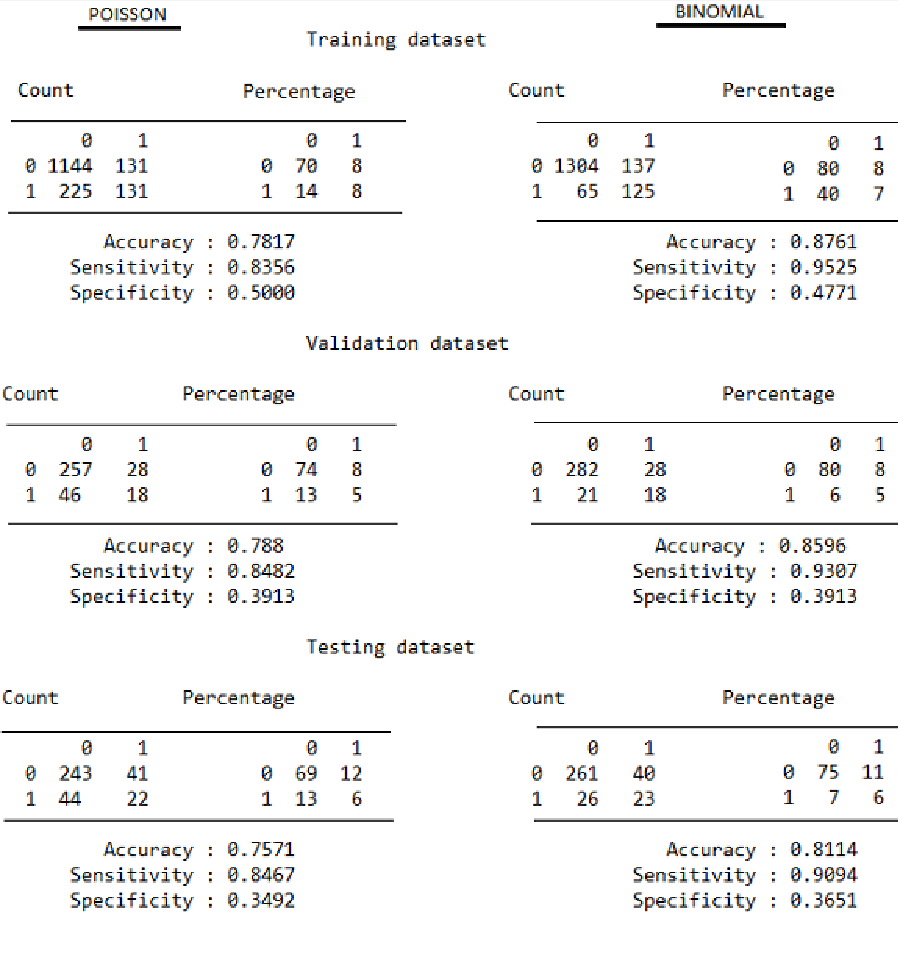
\includegraphics[scale=1.0]{ConfusionMatrix.pdf}
\caption[Confusion (Error) matrices]{Basic comparison of prediction and actuals as confusion matrices using both counts and calculated as a percentage. Summary statistics are computed and displayed}
\label{ConfusionMatricesAll}
\end{figure}

The confusion matrices for the Training, Validation and Testing datasets
for the poisson \textbf{Amodel} that we have previously seen are
displayed obove. Two tables per dataset are displayed, the first list
the actual counts of observations and the second the percentages. We can
observe using the Testing dataset, that for \(69\)\% of the predictions
the model correctly predicts pending or near misses i.e., no pnl loss
impact (called the true negatives). That is, \(243\) out of the \(350\)
loss events are correctly predicted as pending or near misses. similarly
we see that the model correctly predicts OpRisk losses (called the true
positives) on \(6\)\% of the events.\medskip

In terms of how correct the model is, we observe that it correctly
predicts OpRisk losses \(22\) out of the \(66\) events on which losses
actually materialise. This is \(33\)\% accuracy in predicting Oprisk
events. This is called the true positive rate, also know as the recall
of a model. It is a measure of how mant of the actual positives the
model can identify, or how much the model can \emph{recall}. This recall
is also known as the \emph{specificity}. Similarly, the true negative
rate is another measure which also arises and is known as the
\emph{sensitivity} is 85\%.\medskip

We also see \(41\) potential events when we expect pnl loss impacts and
none occur (called the false positives). If we were using this mode to
help us decide whether or not to be wary and closely monitor future
daily trading activity, then there aren't probably serious conscequences
in this instance, we heightened our risk threshold without need. More
serious though is that there are \(44\) actual loss events when our
model tells us there will be no pnl impact yet losses occur (called the
false negatives). We are inconveniently incurring OpRisk losses without
moderating for the risk. Notice that the overall accuracy of the
training dataset is \(78\)\% which is not surprising as the estimated
accuracy of the resulting learned model leads to overoptimistic
estimates due to overspecialisation of the learning algorithm to the
data.

\singlespacing

\doublespacing

\subsection{ROC Curve}

An ROC chart plots the true positives against the false positive rate,
essentially to compare the performance of the model against known
outcomes and is used to identify a suitable trade-off between effor and
outcomes. Generally the larger area-under-curve (auc) also the
probability that the classifier scores a randomly drawn positive sample
higher than a randomly drawn negative sample. For a more comprehensive
comparison, see figure \ref{ROCCurveAll} in Appendix
\ref{sec:Evaluate model performance on the test dataset}.

\begin{figure}
\centering
\begin{subfigure}[b]{0.5\textwidth}
   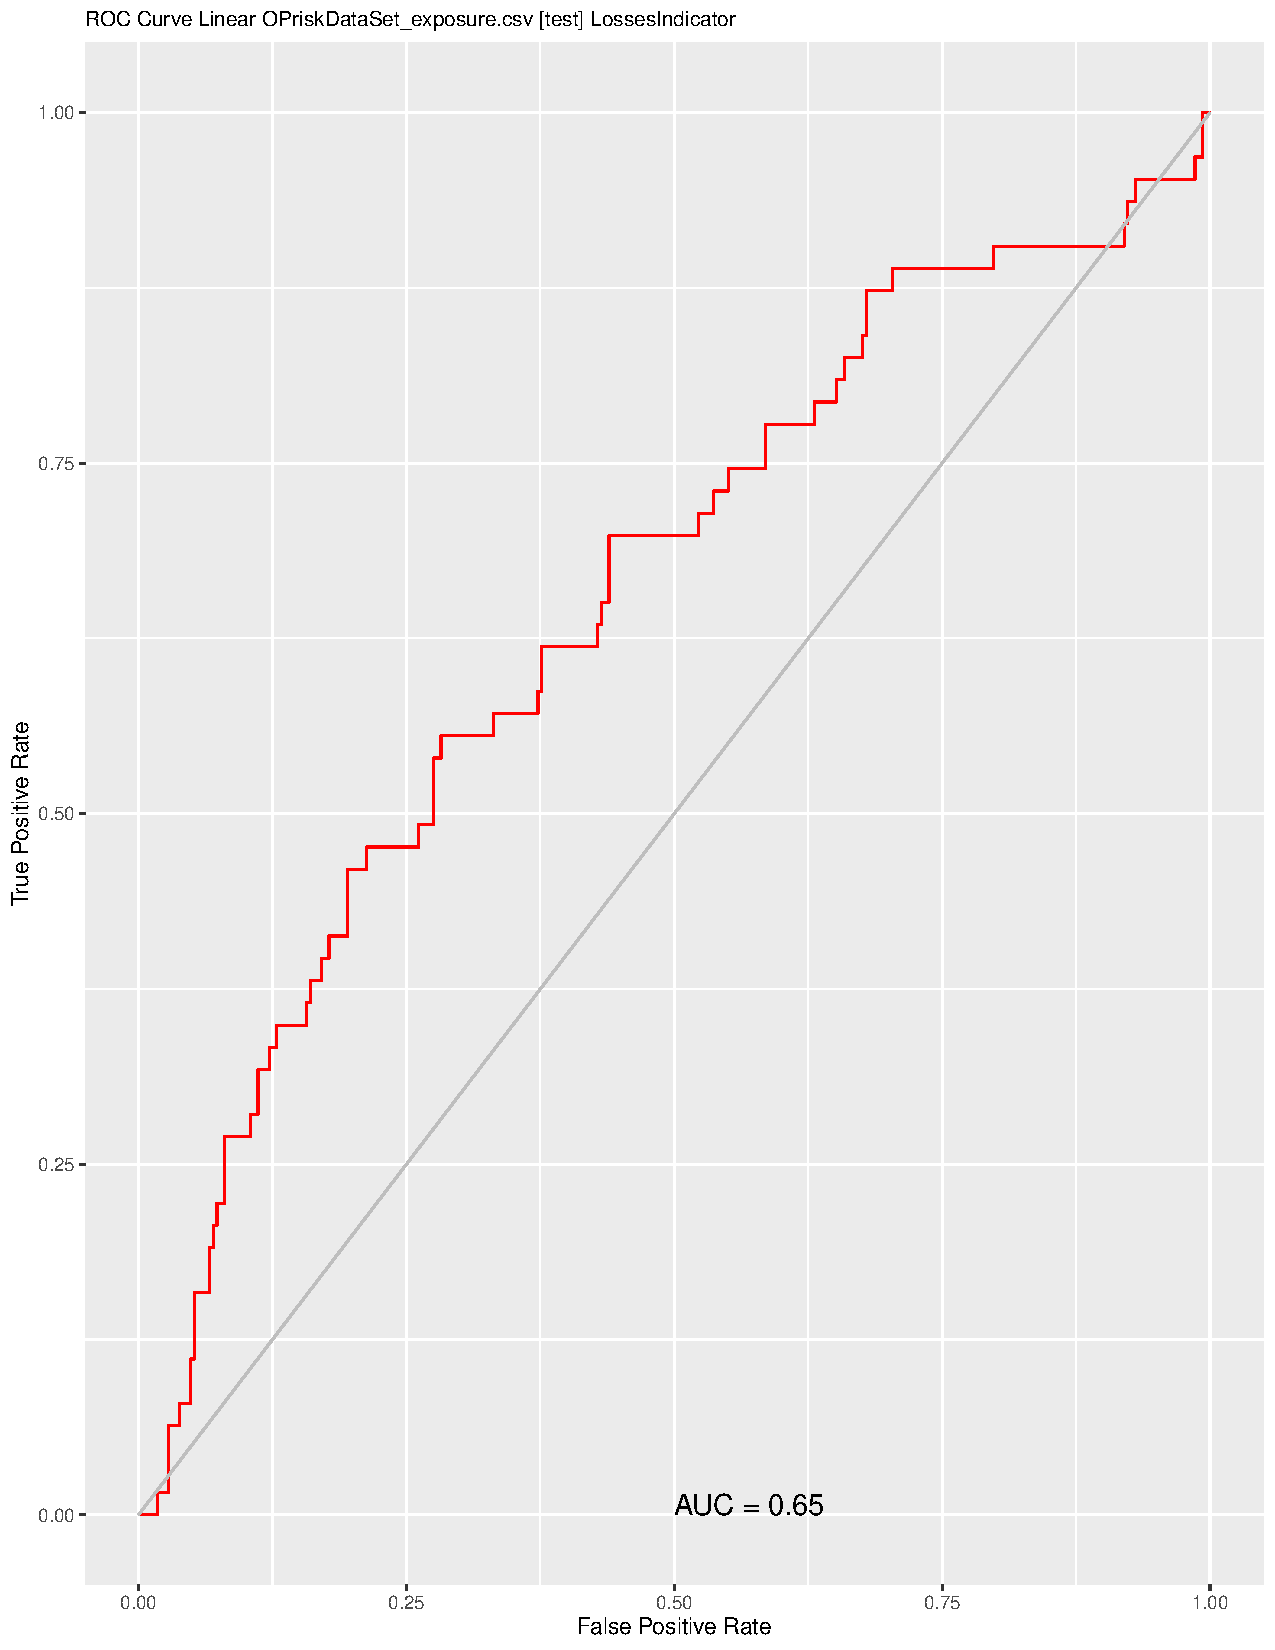
\includegraphics[width=1\linewidth]{ROC_Curve_POITesting.pdf}
   \caption{}
   \label{ROC_Validation_dataset} 
\end{subfigure}

\begin{subfigure}[b]{0.5\textwidth}
   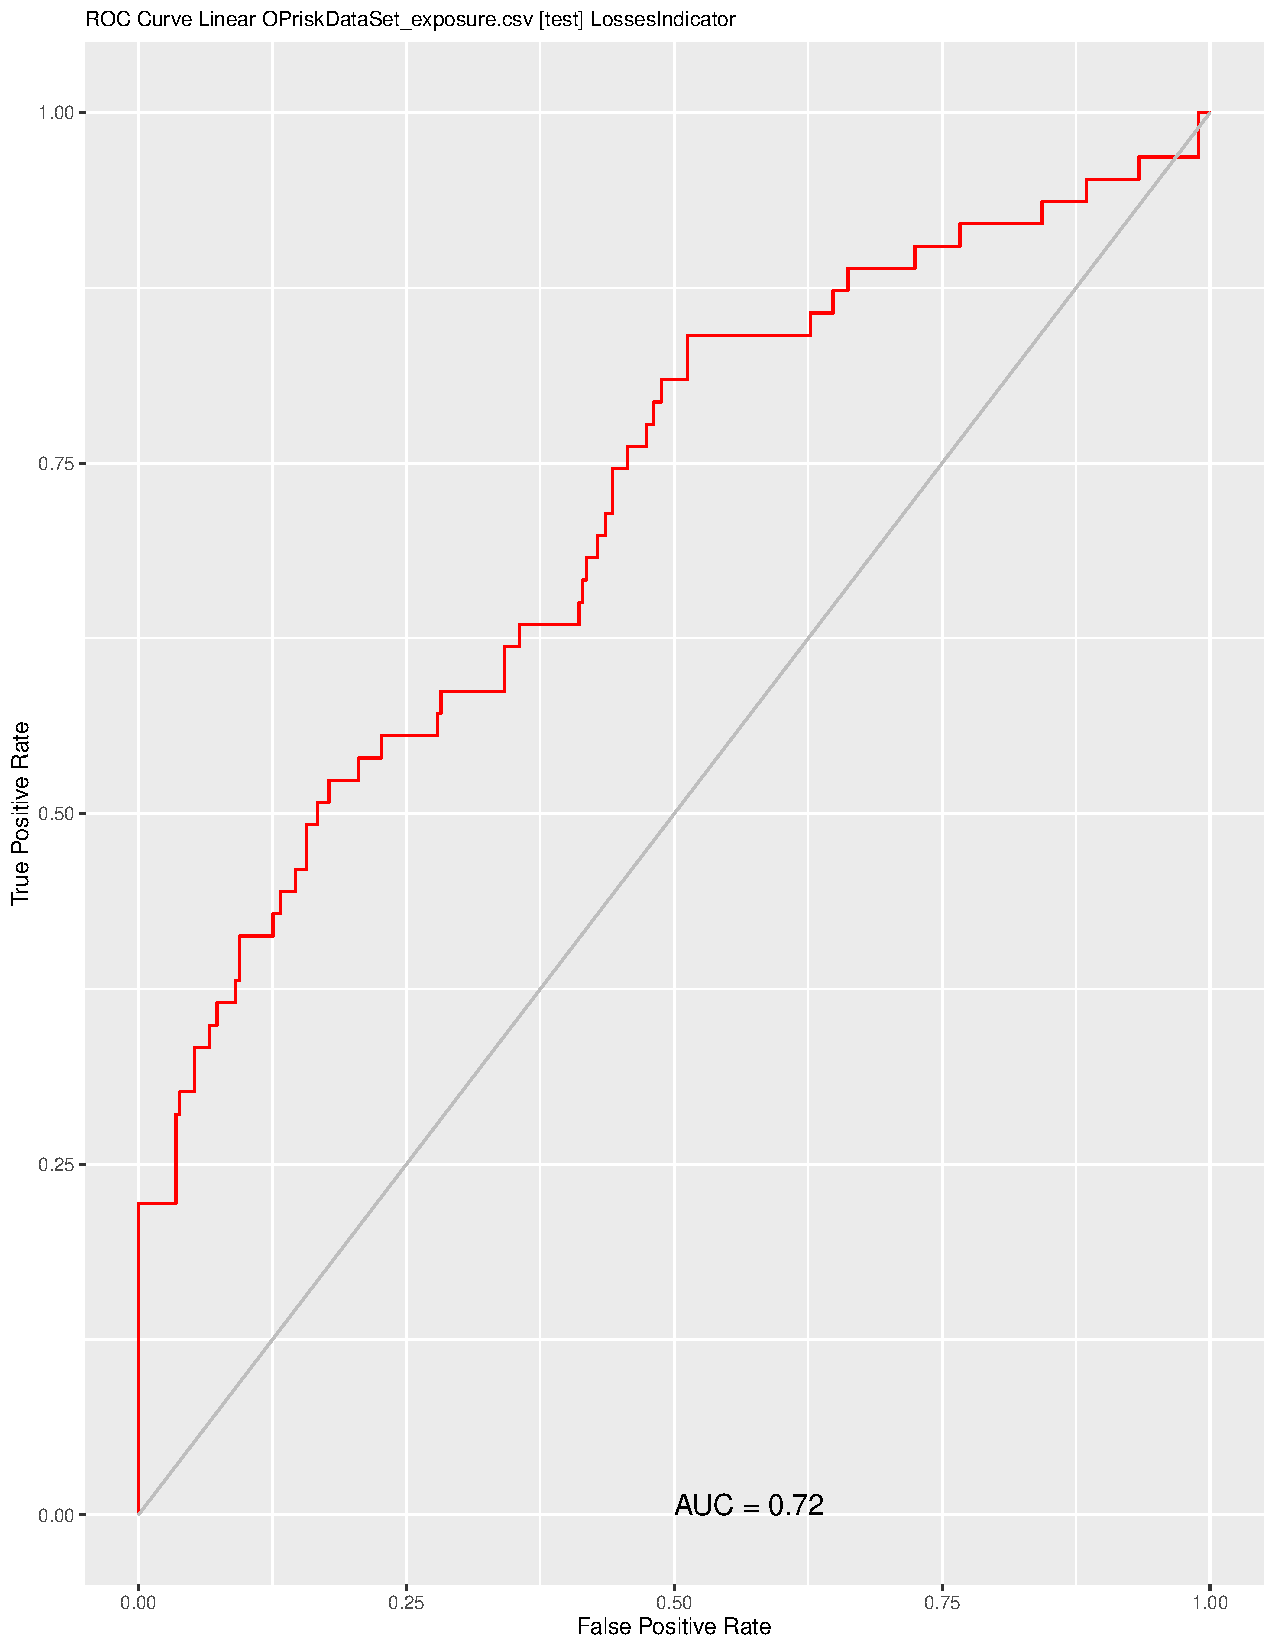
\includegraphics[width=1\linewidth]{ROC _Curve_BINTesting.pdf}
   \caption{}
   \label{ROC_Testing_dataset}
\end{subfigure}

\caption[ROC Curves for GLM over validation and testing set]{(a) ROC Curve for a binomial GLM on the validation dataset (b) As for (a) but on the testing dataset. The area under the curve \texttt{auc} is a measure of the performance of the model. A perfect model would have $100\%$ of the area under the curve}
\end{figure}

\singlespacing

\doublespacing

\subsection{Discussion on MuMIn model performance}
\label{ssec:Discussion on MuMIn model performance}

Conceptually the ``best model'' \textbf{Amodel} represents the phenomena
hypothesised from the information in the observed data, which then forms
the basis for making inferences about the OpRisk frequency processes or
system that generated the data. Multimodel inference leads to even more
robust inferences, especially in the point of view that the selection of
the model used to estimate the mean frequency must, at the same time,
serve the ultimate root cause analysis objective of OpRisk control, that
is to decide when calculating the capital requirement using a robust
OpVaR measurement technique, to take into account as many
characteristics of the trading OpRisk dataset as possible, as well to
consider how the variables interact with each other.\medskip

The performance measures here can ether tell us that we are going to
experience realised losses from OpRisk events more often than we would
like, or overcompensate for losses that do not materialise. This is an
important issue i.e., the fact that the different types of errors have
different conscequences for us. Higher risks (extremal events) are
normally compensated more than necessary and often than not cause social
division within management structures when sectors cannot reconcile or
afford the protection.

\section{Data augmentation}

After monitoring profiling and integration, the known HFLS \& LFHS data
management dilemna needs to be overcome at the last stage, which
requires some innovation. Furthermore, ML algorithms are data driven
therefore the more data the better the model. In the OpRisk context,
problems due to data sensitivity concerns and cost constraints have
limited the study to only three months of available data, which by
implication means increasing the number of data points in some way. One
way of adding to the base data is deriving from the internal sources of
an institution using an extrapolation technique i.e., based on
heuristics the relevant fields are updated or provided with
values.\medskip 

We have a population of \(K = 2330\) OpRisk events over the first
quarter Q12013, and of these events we have a number \(N = 371\) of
realised losses. \(N\) is a discrete random variable modelled as a
Poisson variable with rate \(\lambda\). Each loss \(X_i\) is another
random variable with an underlying sverity distribution. How does the
size \(K\) of the population enter the risk model?. It doesn't appear
explicitly in the model (Parodi, 2014), however, it is taken into
account during the creation of the model. Intuitively, the poisson rate
\(\lambda\) is likely to be proportional to the current OpRisk sample
size, or more specifically, it is the rate of some expected operational
event over per specified time interval.\medskip

\singlespacing

\doublespacing

Predicting test set results and evaluating the parameter \(\lambda\)
Yields a daily rate of \(\lambda = 0.20739163\) per day quarter, which
computes to a cut-off probability of \(0.18009498\). By a simple growth
formula, one years of data (4 quarters) i.e., 3 months * 4 = 1 year:

\singlespacing

\begin{eqnarray}
\mbox{1yr Population} &=& \mbox{Initial Population} + \mbox{Initial Population} * (1 + \lambda)^n \nonumber \\
 &=& 2330 + 2330*(1+0.18009498) + 2330*(1+0.18009498)^2 \nonumber \\
 &+& 2330*(1+0.18009498)^3\nonumber \\
 &=& 11,791 \mbox{observations}
\end{eqnarray} \doublespacing

This corresponds to a 1yr population of \(11,791\) observations. The
next step is to use an extrapolation script to generate the \(11,791\)
observations for the augmented dataset. The extrapolation algorithm
which augments the existing data to increase the size of the population
by the heuristics approach, effectively increasing the number of rows,
which is best done in the Matlab code (due to it's matrix based
foundations), see section
\ref{sec:Data augmentation code: Extrapolation simulation in Matlab} on
page
\pageref{sec:Data augmentation code: Extrapolation simulation in Matlab}in
the Appendix \ref{sec:Appendix B: R Code for Chapter 4}.

\subsection{Deploying the R model}
\label{ssec:Deploying and R model}

Often for one to obtain the benefit of a model, it's ``scored'' through
applying it to a new dataset using a form of a predict() function. This
is the simplest approach to deployment and is practiced regularly as new
data entries become available, particularly using the R concept, whereby
model outcomes are saved for later use then at a later time a new
dataset scored using the saved model and applying it to some new data
enhancing the data mining capabilities within an organisation. \medskip

After building the augmented dataset we simulate the application of the
model to it. We can then schedule the model to be applied regularly as
new data points come in, spurring off secondary and tertiary processes
such as the flagging of potentially hazardous future events, high risk
individuals or perhaps identifying clients who need to be audited or to
communicate to the trader the predicted critical risk indicators for
tomorrow.

\singlespacing

\doublespacing

\section{The estimation of some  generalised additive models for location scale and shape (GAMLSS) for severity loss estimation}
\label{sec:The estimation of some  generalised additive models for location scale and shape (GAMLSS) for severity loss estimation}

Figure \ref{fourLossplot1} and \ref{fourLossplot2} shows plots of the
pnl impact, \texttt{Loss}, against three selected explanatory variables
chosen for the purpose of demonstrating the complexity of their
relationship, hence the need for a statisical model for the analysis of
the OpRisk data viz., GAMLSS. In the first two plots labelled figure
\ref{fourLossplot1} (a) for the two explanatory variables in the
bivariate plots, \texttt{Loss} vs \texttt{UpdatedTime} and \texttt{Loss}
vs \texttt{UpdatedDay}, there is obvious nonlinear dependence between
the mean of the response variable Loss and the \texttt{UpdatedTime} and
\texttt{UpdatedDay}, here nonparametric smoothing functions may be
needed. There is also a clear indication of the non-homogeniety of the
variance of Loss, therefore modelling the variance of \texttt{Loss}
requires a statistical model which caters for the dependency of the
variance of its's mean and/or explanatory variables.\medskip

\singlespacing

\doublespacing

The first boxplot displays how the day in the month \texttt{UpdatedDay}
varies according to the OpRisk event, and the second how the
\texttt{Loss} varies according according to same. There is clear
indication of positive skewness in the distribution of \texttt{Loss}
depending on the explanatory variable \texttt{EventTypeCategoryLevel},
and asymmetrical boxes about the median a nd long upper and lower
whiskers, especially in the first boxplot, emphasizing the need to
explicitly modelfor this.

\begin{figure}
\centering
\begin{subfigure}[b]{0.5\textwidth}
   \includegraphics[width=1\linewidth]{Rplot01.eps}
   \caption{Plots of \texttt{Loss} against explanatory variables }
   \label{fourLossplot1} 
\end{subfigure}

\begin{subfigure}[b]{0.5\textwidth}
   \includegraphics[width=1\linewidth]{Rplot.eps}
   \caption{Boxplots of \texttt{UpdatedDay} and \texttt{Loss} against explanatory variable \texttt{EventtypeCategoryLevel1}}
   \label{fourLossplot2}
\end{subfigure}

\caption[Loss against explanatory variables]{(a) Plot of the Loss (pnl impact) against explanatory variables UpdatedTime and UpdatedDate. (b) As for (a) against EventTypeCategory.}
\end{figure}

\subsection{Model strategy in GAMLSS framework}

The OpRiskDataSet\_exposure data contains intra-day pnl impacts (Losses)
of amendment activity of during trading across primary and secondary
markets of an investment banking platform. We use model selection to
discover the effect of pnl losses i.e., fitting different distributions
to the response variable in order to select a plausible distribution for
the GAMLSS. Let
\(\mathcal{M}=\{\mathcal{D},\mathcal{G},\mathcal{T},\Lambda\}\)
represent Stasinopoulos et al. (2018)'s expansion of equation
\ref{EqnGAMLSS}. Teh components of \(\mathcal{M}\) are defined as
follows (Voudouris, Gilchrist, Rigby, Sedgwick, \& Stasinopoulos, 2012):

\begin{enumerate}
\item $\mathcal{D}$ specifies the distribution of the response variable,
\item $\mathcal{G}$ specifies the link functions,
\item $\mathcal{T}$ specifies the terms appearing in all the predictors for $\mu,\sigma,\nu$ and $\tau$,
\item $\Lambda$ specifies the smoothing hyper-parameters which determine the amount of smoothing in the $h_{kj}()$ functions of equation
\ref{EqnGAMLSS}.
\end{enumerate}

\subsection{Component $\mathcal{D}$: Selection of the distribution}

We begin model selection using only three distribution parameter
distribution otherwise known as the Lambda, Nu and Sigma (LMS) method
(Stasinopoulos et al., 2018) selected from the family of zero adjusted
distributions; on zero and the positive real line \([0,\infty)\), and
then move to its extensions (four distribution parameters). Of the zero
adjusted distributions, only the Zero adjusted gamma
\(\mbox{ZAGA}(\mu,\sigma,\nu )\) and the zero adjusted inverse gamma
\(\mbox{ZAIG}(\mu,\sigma,\nu )\) can be fitted explicitly in GAMLSS,
therefore we begin with this in mind. The parameters \(\mu,\sigma\) and
\(\nu\) in this case, are the approximate mean, approximate coefficient
of variation and skewness parameters.\medskip  

\singlespacing

\doublespacing

The introduction of a fourth parameter \(\tau\) for modelling the
kurtosis of the distribution leads to the creation of the generalized
beta type 2 distribution, denoted by
\(\mbox{GB}2(\mu, \sigma,\nu,\tau)\), which is the only four parameter
distribution for fitting a GAMLSS to estimate the (non-linear nature)
mean OpRisk loss severity explicity.

\subsubsection{Generalized Beta type $2$ distribution (GB$2$)}

Given \(X=x\), \(Y\) (the \texttt{Loss} severity is the target variable)
is modelled here by a generalized beta type 2
\(\mbox{GB}2(\mu, \sigma,\nu,\tau)\)\footnote{The GB2 adjusts the obove density $f(y|\mu,\sigma,\nu,\tau)$, resulting from the condition $y>0$, where $\mu>0$, $-\infty<\sigma<\infty$, $\nu>0$ and $\tau>0$. The mean and the variance of $Y$ are given by $E(Y)=\mu\mbox{B}(\nu+\frac{1}{\sigma},\tau-\frac{1}{\sigma})/\mbox{B}(\nu,\tau)$ for $-\nu<\frac{1}{\sigma}<\tau$ and $E(Y^2)=\mu^2\mbox{B}(\nu+\frac{2}{\sigma})/\mbox{B}(\nu,\tau)$ for $-\nu<\frac{2}{\sigma}<\tau$, See @stasinopoulos2008instructions.}
distribution is defined by:

\singlespacing

\begin{eqnarray}\label{EqnPdfGB2}
f(y|\mu,\sigma,\nu,\tau)=|\sigma|y^{\sigma\nu-1}\{\mu^{\sigma\nu}\mbox{B}(\nu,\tau)[1+(y/\mu)^{\sigma}]^{\nu+\tau}\}^{-1}
\end{eqnarray} \doublespacing

\singlespacing

\doublespacing

The choice of distribution for the OpRisk severity \texttt{Loss}
variable is based on it being the only simple explicit for the mean and
median of the response variable. Additionally:-

\begin{list}{*}{}
\item The variate takes values within to the appropriate range viz., $[0,\infty)$;
\item The distribution is relevant because in has an explicit p.d.f, c.d.f and inverse c.d.f, explicit moment based measures of location, scale, skewness and kurtosis (i.e. population mean, standard deviation, $\gamma_1, \gamma_2$ [@rigby2017distributions]);
\item Explicit centiles and centile based measures viz., median, semi-interquartile range, skewness and kurtosis ($\gamma, \mbox{st}_{0.49}$ resp.);
\item Continuity of $f(y|\mu,\sigma,\nu,\tau)$ w.r.t y and it's derivatives w.r.t $\mu,\sigma,\nu,\tau$;
\item Allows for flexibility in specifying the distribution of severity and also allowing for the modelling of distribution parameters as function of explanatory variables
\end{list}

\section{GAMLSS model for the four parameters of the $\mbox{GB}2$ distribution}

The parameters \(\mu, \sigma,\nu,\) and \(\tau\) of the \(\mbox{GB}2\)
distribution are modelled as functions of explanatory variables using
semi-parametric additive models, extended to incorporate non-linear
parametric and/or non-parametric smooth functions \(x\). Specifically,
the model assumes that conditional on \((\mu_i,\sigma_i,\nu_i,\tau_i)\),
for \(i=1,2,\ldots,n\), observations where
\(Y \sim \mbox{GB}2(\mu,\sigma,\nu,\tau)\) i.e., \(Y_i\) are independent
\(\mbox{GB}2(\mu_i,\sigma_i,\nu_i,\tau_i)\) variables with p.d.f
\(\mathcal{f}_{Y_i}(\mathcal{y}_i)\) obtained from equation
\ref{EqnPdfGB2}.

\subsection{Component $\mathcal{G}$: selection of the link functions}

Also for \(k=1,\ldots,4\) let \(g_k(\cdot)\) be known momotonic link
functions relating the parameters to expalnatory variables through
extended semi-parametric additive models given by:

\singlespacing

\begin{eqnarray}\label{EqnLinks}
g_1(\mu) &=& \eta_1 = \mathbf{\Large{X}}_1\mathbf{\beta}_1 + \sum_{j=1}^{J_1}h_{1j}(\mathbf{x}_{1j})\nonumber\\
g_2(\sigma) &=& \eta_2 = \mathbf{\Large{X}}_2\mathbf{\beta}_2 + \sum_{j=1}^{J_2}h_{2j}(\mathbf{x}_{2j})\nonumber\\
g_3(\nu) &=& \eta_3 = \mathbf{\Large{X}}_3\mathbf{\beta}_3 + \sum_{j=1}^{J_3}h_{3j}(\mathbf{x}_{3j})\nonumber\\
g_4(\theta) &=& \eta_4 = \mathbf{\Large{X}}_4\mathbf{\beta}_4 + \sum_{j=1}^{J_4}h_{4j}(\mathbf{x}_{4j})
\end{eqnarray} \doublespacing

where for \(i=1,2,\ldots,n\) \(j=1,2,\ldots,J_k\) and
\(\mathbf{\beta}_k^T=(\beta_1k,\beta_2k,\ldots,\beta_{J'_kk})\) is a
parametric vestor of length \(J'_k\), \(\mathbf{x}_{ik}\) a fixed known
design vector of length \(J''_k\) and \(h_k\) a non-linear function
{[}{]}. The explanatory values \(x_{jk}\) are assumed to be fixed and
known and the univariate function \(h_{jk}\) is an additive smooth
parametric function assumed to have continuous first and second order
derivatives. If for \(k=1,2,3,4\), \(J_k=0\), then the GAMLSS model
\ref{EqnLinks} reduces to a non-linear parametric model. If in addition,
\(h_k(x_{ik},\mathbf{\beta}_k)=\mathbf{x}_{ik}^T\mathbf{\beta}_k\) for
\(i=1,2,\ldots,n\) and \(k=1,2,3,4\), then equation \ref{EqnLinks}
reduces to a linear parametric model (Rigby, Stasinopoulos, Heller, \&
De Bastiani, 2017).

\section{Model estimation and selection}
\label{sec:Model estimation and selection}

There are several different strategies that could be applied for model
selection of the terms used to model the four parameters, however the
procedure in the analysis as outlined in Stasinopoulos et al. (2018) and
Voudouris et al. (2012), comprised of the function \texttt{stepGAIC.A},
is by selcting all terms for all the parameters by a forward, backward
or stepwise procedure, assuming the particular response distribution
function (also found in Stasinopoulos, Rigby, Heller, Voudouris, \& De
Bastiani, 2017 \& @rigby2017distributions). The final model may contain
different combinations for \(\mu, \sigma,\nu,\) and \(\tau\).

\subsection{Component $\mathcal{T}$ and $\Lambda$: selection of the terms and smoothing parameters in the model}

Given that a set of plausible distributions have been identified, let
\(\chi\) be the selection of all terms available for consideration.
Their parameters are modelled as regression models. In particular the
non-linear parameter vectors \(\mathbf{\beta}_k\) and the non-parametric
functions \(h_{jk}\) for \(j=1,2,\ldots,J_k\) and \(k=1,2,3,4\) in
equation \ref{EqnLinks} are estimatied by maximizing the penalised
log-likelihood as a way of understanding how the location, scale,
skewness and kurtosis parameters of the loss severity distribution are
affected by the explanatory variables.\medskip

This is essentially shown conducted, in R, dropping unneccessary terms,
selecting and adding additive terms and smoothing terms. In order to do
this a formula is created containing all the linear main effects and
second-order interactions plus smooth function of expalnatory variables.
In R this is achieved through a ``scope'' statement whereby the function
\texttt{FORM} is used as the upper argument, as demonstrated in see
Appendix \ref{sec:Selection of terms.}.

\singlespacing

\doublespacing

\section{Checking the model}

Figure \ref{4Residual_GOF_plot} displays the (normalized quantile)
residuals, from model \(\mbox{GB}2()\). Panel \((a)\) and \((b)\) plot
the residuals against the fitted values of \(\mu\) and against the
explanatory variables respectively. While panel \((c)\) and \((d)\)
provide a kernel density estimate and normal \(\mbox{QQ}\) plot for them
respectively. the residuals appear slightly skewed to the right and the
\(\mbox{QQ}\) plot shows extreme outliers in the upper tails of the
distribution of \(y\). Also note that not all plots in figure
\ref{4Residual_GOF_plot} are useful, nevertheless the \(\mbox{GB}2\)()
distribution model provides a reasonable fit to the data, substantially
better than to the and preferable to the models.

\begin{figure}
\centering
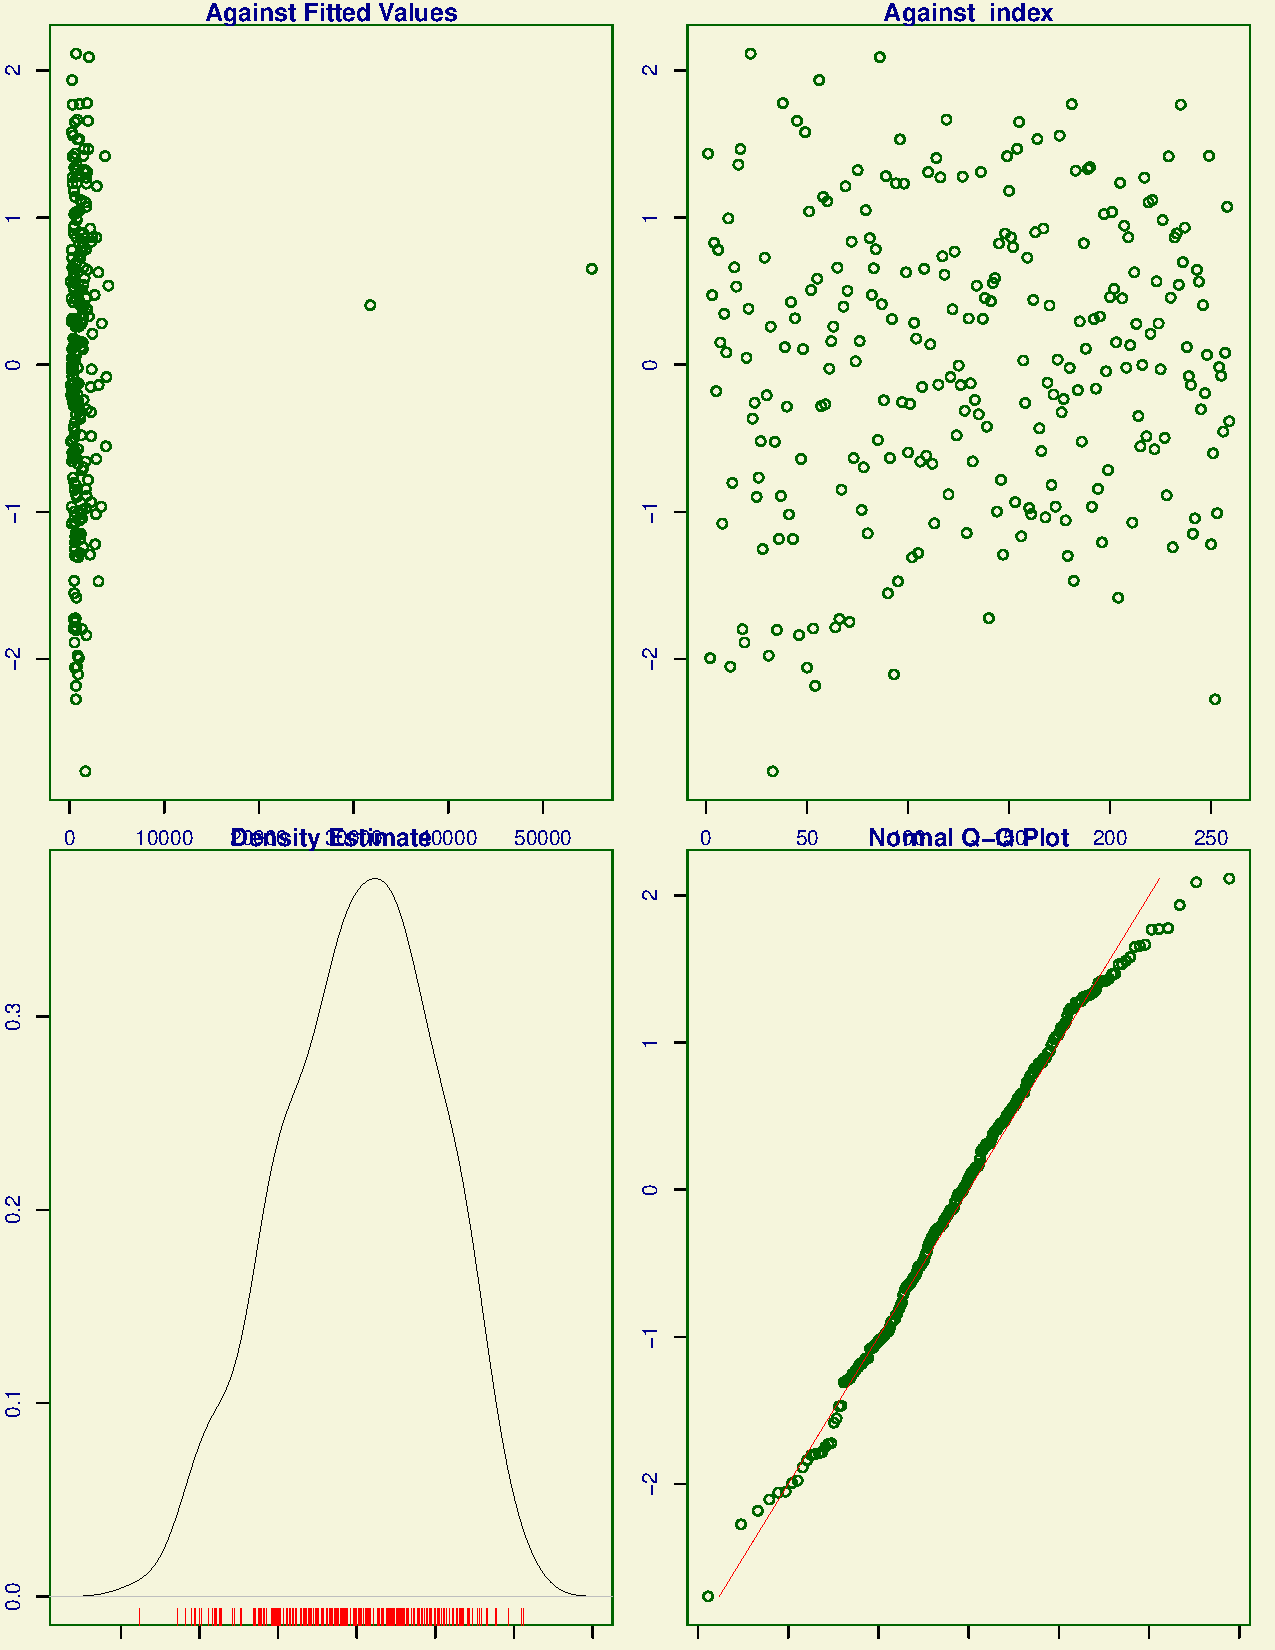
\includegraphics[height=10cm, width=10cm]{4_GOF_plot.pdf}
\caption[Normalized quantile residuals from model $\mbox{GB}2$]{The result of the plot displays (normalized quantile) residuals from model $\mbox{GB}2(\mu,\sigma,\nu,\tau)$, the top-left panel plots the residuals against the fitted values of $\mu$, the bottom-left panel provides a kernel density estimate and the normal QQ plot for the residuals in bottom-right panel. The last panel results are meaningless}.
\label{4Residual_GOF_plot}
\end{figure}

\singlespacing

\doublespacing

\begin{figure}
\centering
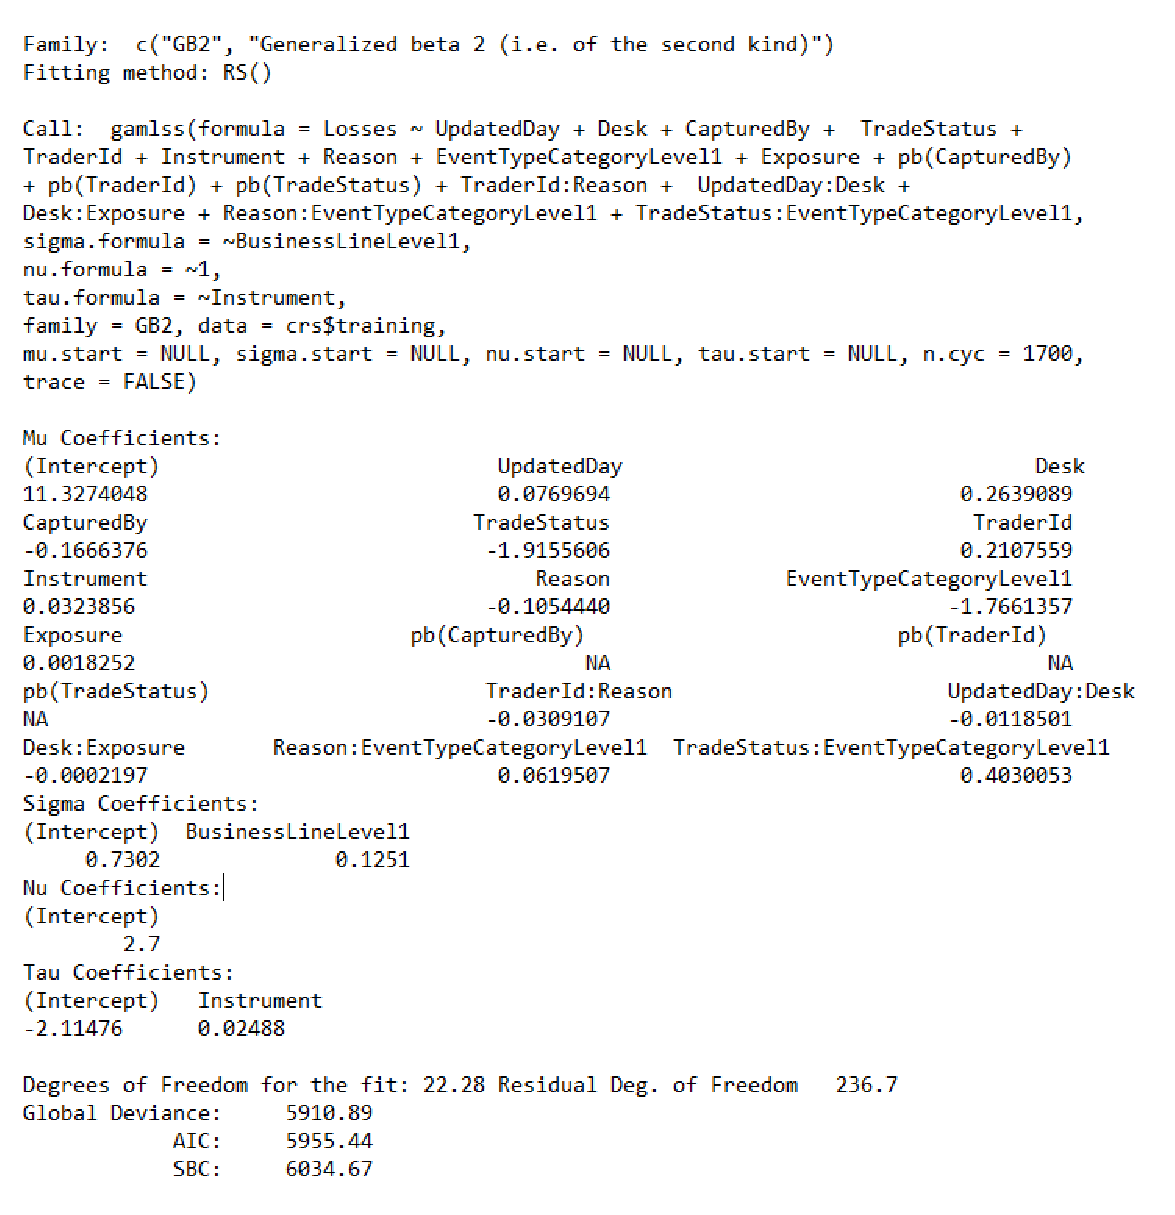
\includegraphics[scale=0.9]{mod42GB2.eps}
\caption[Summary of fitted distribution]{Summary statistics of fitted distribution $\mbox{GB}2(\mu,\sigma,\nu,\tau)$, the "Generalized beta type 2 (i.e. of the second kind)" using fitting method: RS()}
\label{SumGB2Anova}
\end{figure}

Figure \ref{SumGB2Anova} shows summary statistics of the \(\mbox{GB}2\)
distribution model. The \(\mbox{GB}2\) distribution is the best fit for
the data based on the model selection strategy discussed in section
\ref{sec:Model estimation and selection}, the empirical GAMLSS-based
model \(Y \sim \mbox{GB}2(\mu,\sigma,\nu,\tau)\) where \(Y=\) log(Losses
due to OpRisk events) and

\small
\singlespacing

\begin{eqnarray}
&\mbox{log}(\mu)& = \mbox{\texttt{UpdatedDay}} + \mbox{\texttt{Desk}} + \mbox{\texttt{CapturedBy}} +  \mbox{\texttt{TradeStatus}} + \mbox{\texttt{TraderId}} + \mbox{\texttt{Instrument}}\nonumber\\
&+& \mbox{\texttt{Reason}} + \mbox{\texttt{EventTypeCategoryLevel1}} + \mbox{\texttt{Exposure}} + \mbox{pb}(\mbox{\texttt{CapturedBy}}) + \mbox{pb}(\mbox{\texttt{TraderId}})\nonumber\\
&+& \mbox{pb}(\mbox{\texttt{TradeStatus}}) + \mbox{\texttt{TraderId:Reason}} +  \mbox{\texttt{UpdatedDay:Desk}} + \mbox{\texttt{Desk:Exposure}}\nonumber\\
&+& \mbox{\texttt{Reason:EventTypeCategoryLevel1}} + \mbox{\texttt{TradeStatus:EventTypeCategoryLevel1}},\nonumber\\
&\sigma& = \mbox{\texttt{BusinessLineLevel1}},\nonumber\\
&\mbox{log}(\nu)& = 1,\nonumber\\
&\mbox{log}(\tau)& = \mbox{\texttt{Instrument}}
\end{eqnarray} \doublespacing \normalsize

\subsection{Testing hypothesis from the fitted model}

Using the \texttt{stepGAIC.A}() function in GAMLSS, we compare the
models tat best fit the 2013Q1 dataset of OpRisk losses, pending and
near misses, conditional on the available explanatory variables such as
the \texttt{UpdatedDay}, \texttt{UpdatedTime}, \texttt{CapturedBy},
\texttt{TraderId}, \texttt{Reason}, \texttt{Desk}, \texttt{Instrument},
etc. The conclusion from Table \ref{GAIC} is that the \(\mbox{GB}2\)
model provides the best fit to expalnatory variables according to
criterion \texttt{GAIC()} i.e., loss severity (pnl impact) requires
modelling of both skewness and kurtosis and is not adequately modelled
by either skewness or kurtosis alone. The fitted models for
\(\mu,\sigma,\nu\) and \(\tau\), given by equation \ref{EqnLinks} for
the chosen model is displayed.

\begin{figure}
\centering
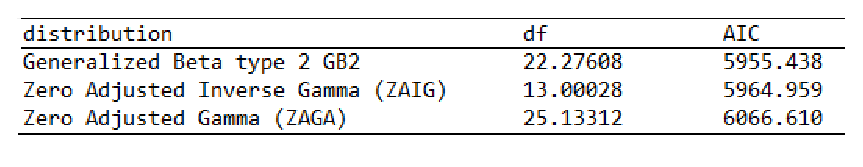
\includegraphics[scale=1.0]{GAIC.eps}
\caption[Summary of fitted models]{Summary of the fitted models for the OpRisk 2013Q1 data, showing the effective degrees of freedom (df) used in the model and the AIC($k=$length of loss variable).}
\label{GAIC}
\end{figure}

\singlespacing

\FloatBarrier
\newpage
\fancyhead[L]{Modeling OpRisk Depending on covariates}
\fancyhead[R]{\thepage}
\fancyfoot[C]{}

\chapter{METHODS FOR MODELING OPRISK DEPENDING ON COVARIATES}
\label{METHODS FOR MODELING OPRISK DEPENDING ON COVARIATES}

\doublespacing

\section{Introduction}
\label{sec:Introduction}

This section of the paper concentrates on combining various supervised
learning techniques with extreme value theory (EVT) fitting, which is
very much based on the Dynamic EVT-POT model developed by
Chavez-Demoulin et al. (2016). This can only happen due to an abundance
of larger and better quality datasets and which also benefits the loss
distribution approach (LDA) and other areas of OpRisk modeling. In
Chavez-Demoulin et al. (2016), they consider dynamic models based on
covariates and in particular concentrate on the influence of internal
root causes that prove to be useful from the proposed methodology.

Motivated by the abundance of data and better data quality, these new
data-intensive techniques offer an important tool for ORM and at the
same time supporting the call from industry for a new class of EBOR
models that capture forward-looking aspects of ORM (Embrechts et al.,
2018). Three different machine learning techniques viz., decision trees,
random forest, and neural networks, will be employed using R. A
comprehensive list of user defined variables associated with root causes
that contribute to the accumulation of OpRisk events (frequency) has
been provided, moreover, a lot can be gained from this dataset as it
also bears the impacts of these covariates on the severity of OpRisk.

\section{Modeling Oprisk: The loss distribution approach (LDA)}
\label{sec:Modeling Oprisk: The loss distribution approach (LDA)}

Machine Learning (ML) is used as a substitute tool for the traditional
model based Autoregressive Moving Average (ARMA) used for analysing and
representing stochastic processes. As opposed to the statistical tool,
ML does not impose a functional relationship between variables, the
functional relationship is determined by extracting the pattern of the
training set and by learning from the data observed.\medskip 

Using computationally intensive (using ML techniques on historical data
) OpRisk measurement techniques and mixing with a theory is not a new
approach for modeling, particularly in calculating OpRisk RC; as
evidenced through Agostini et al. (2010) in a study whereby the LDA
model for forecasting OpRisk RC, via VaR, was implemented in conjunction
with the use of advanced credibility theory (CT). The idea at the basis
of their use of CT, is to advance the very recent literature that a
better estimation of the OpRisk RC measurement can be obtained by
integrating historical data and scenario analysis i.e., combining the
historical simulations with scenario assessments through formulas that
are weighted averages of the historical data entries and scenario
assessments, advocating for the combined use of both
experiences.\medskip 

However, applying ML is an original way of looking at the approximation
issue as opposed to advanced CT. The essential feature of PT are
assumptions which are more compatible with basic principles of
perception and judgement for decisions taken under uncertainty, whereas
ML will reveal additional chance probabilities determined through the
natural clusters of unknown data feature findings from which new
discoveries are made.\medskip

Twenty-one key risk indicators (kri's) with eight feature groups
including person identification, trade origination, root causes and
market value sensitivities are in the chosen covariates. For each risk
event there is information about: trading risk exposure, trading
characteristics, causal factor characteristics and the losses created by
these factors. The development, training and validation of the machine
learning (ML) models lends itself to this new type of data and requires
a higher degree of involvement across operations. Moreover, at this
level of granularity the different types of data is particularly suited
to exposure-based treatment, and other forward-looking aspects within
the OpRisk framework, for improved forecasts of OpRisk losses.\medskip

The aggregated operational losses can be seen as a sum \(S\) of a random
number \(N\) individual operational losses \[(X_1, \ldots, X_N )\]. The
total required capital is the sum of VaR of each BL/ET combination
calibrated through the underlying mathematical model whose analytic
expression is given by:

\singlespacing

\begin{equation}\label{eqn4}
\mathbf{G}_{\vartheta(t)}(x)=Pr[\vartheta(t)\leq x]=Pr\left(\sum_{n=1}^{N(t)}X_{n} \leq x\right), \qquad \mbox{where} \quad \vartheta(t) = \sum_{n=1}^{N(t)} X_{n}.
\end{equation} \doublespacing

\(\mathbf{G}(t)\) can only be obtained numerically using the Monte Carlo
method, Panjer's recursive approach, and the inverse of the
characteristic function (Frachot et al. (2001); Aue \& Kalkbrener
(2006); Panjer (2006); \& others).

\subsection{Research Objective II}

To test the accuracy of several classes of data-intensive techniques in
approximating the weights of the risk factors; i.e., the input features
of the model viz., TraderID, UpdatedDay, Desk, etc. of the underlying
value-adding processes, against traditional statistical techniques, in
order to separately estimate the frequency and severity distribution of
the OpRisk losses from historical data. As a consequence, capital
estimates should be able to adapt to changes in the risk profile e.g.,
upon the addition of new products or varying the business mix of the
bank (e.g., terminations, voids, allocations, etc.) to provide
sufficient incentives for ORM to mitigate risk (Einemann et al., 2018).

\section{Analysis and interpretation issues with behavioral finance theory}
\label{sec:Analysis and interpretation issues with behavioral finance theory}

Behavioral management theory is very much concerned with social factors
such as motivation, support and employee relations. A critical component
of behavioral finance is building models which better reflect actual
behavior. Studies have revealed that these social factors are not easy
to incorporate into finance models or to understand in the traditional
framework.\medskip 

The traditional finance paradigm seeks to understand financial markets
using models in which agents are \lq\lq rational\rq\rq. According to
Barberis \& Thaler (2003), this means that agents update their beliefs
on the onset of new information, and that given their beliefs, they make
choices that are normatively acceptable, and that most people do this
most of the time. Neoclassical theory has grown to become the primary
take on modern-day economics formed to solve problems for decision
making under uncertainty/risk. Expected Utility Theory (EUT) has
dominated the analysis and has been generally accepted as the normative
model of rational choice, and widely applied as a descriptive model of
economic choice (Kahneman \& Tversky, 2013).

\subsection{Expected utility theory}
\label{ssec:Expected utility theory}

Expected utility
theory\footnote{Expected utility theory provides a model of rationality based on choice.}
(EUT): We see a fundamental relation for expected utility (Expectation)
of a contract \(X\), that yields outcome \(x_i\) with probability
\(p_i\), where \(X = (x_1,p_1; ...; x_n,p_n)\) and
\(p_1+p_2+\ldots+p_n=1\) given by:

\singlespacing

\begin{equation}\label{EUT_extended}
U(x_1,p_1;\ldots;x_n,p_n) = p_1u(x_1)+\ldots+p_nu(x_n) 
\end{equation} \doublespacing corroborated by Morgenstern \& Von Neumann
(1953); Friedman \& Savage (1948); Kahneman \& Tversky (2013) \& others.

A common thread running through the rational viz., the neoclassical take
of modern-day economics vs the non-neoclassical schools of thought are
findings of behavioral economics which tend to refute the notion that
individuals behave rationally. Many argue that individuals are
fundamentally irrational because they do not behave rationally giving
rise to a literature and debates as to which heuristics and sociological
and institutional priors are rational (Altman, 2008).\medskip

In the real world there is a point of transition between the traditional
(neoclassical) approach to decision making, based on data and data
anaysis (logic and rational), by adding new parameters and arguments
that are outside rational conventional thinking but are also valid. For
example, that neoclassical theory makes use of the assumption that all
parties will behave rationally overlooks the fact that human nature is
vulnerable to other forces, which causes people to make irrational
choices.\medskip 

An essential ingredient of any model trying to understand trading
behavior is an assumption about investor preferences (Barberis \&
Thaler, 2003), or how investors evaluate risky gambles. Investors
systematically deviate from rationality when making financial decisions,
yet as acknowledged by Kuhnen \& Knutson (2005), the mechanisms
responsible for these deviations have not been fully identified. Some
errors in judgement suggest distinct mental operations promote different
types of financial choices that may lead to investing mistakes.
Deviations from the optimal investment strategy of a rational risk
neutral agent are viewed as risk-seeking mistakes and risk-aversion
mistakes (Kuhnen \& Knutson, 2005).\medskip 

\subsection{Theoretical investigations for the quantification of moderm ORMF}

Kuhnen \& Knutson (2005) explain that these risk-seeking choices (such
as gambling at a casino) and risk-averse choices (such as buying
insurance) may be driven by distinct
neural\footnote{As recent evidence from human brain imaging has shown [@kuhnen2005neural] linking neural states to risk-related behaviours [@paulus2003increased].}
phenomena, which when activated can lead to a shift in risk preferences.
Kuhnen \& Knutson (2005) found that certain areas of the brain precede
risk-seeking mistakes or risky choices and other areas precede
risk-aversion mistakes or riskless choices. A risk-aversion mistake is
one where a gamble on a prospect of a gain is taken by a risk-averse
agent in the face of the chance of a prospective loss. The fear of
losing prohibits one's urge to gamble, but people engage in gambling
activity anyway. Barberis \& Thaler (2003) show that people regularly
deviate from the traditional finance paradigm evidenced by the extensive
experimental results compiled by cognitive psycologists on how people
make decisions given their beliefs.\medskip 

Kahneman \& Tversky (2013) maintains, preferences between prospects
which violate rational behaviour demonstrate that outcomes which are
obtained with certainty are overweighted relative to uncertain outcomes.
This will contribute to a risk-averse preference for a sure gain over a
larger gain that is merely probable or a risk-seeking preference for a
loss that is merely probable over a smaller loss that it certain. As a
psycological principle, overweighting of certainty favours risk-aversion
in the domain of gains and risk-seeking in the domain of losses.\medskip

The present discussion replicates the common behavioral pattern of risk
aversion, where people weigh losses more than equivalent gains.
Furthermore, neuroeconomic research shows that this pattern of behavior
is directly tied to the brain's greater sensitivity to potential losses
than gains (Tom, Fox, Trepel, \& Poldrack, 2007). This provides a target
for investigating a more comprehensive theory of individual
decision-making rather than the rational actor model and thus yield new
insights relevant to economic
theory\footnote{Representing ability of FI's financial market models to characterise the repeated decision-making process that applies to loss aversion}
(Kuhnen \& Knutson, 2005).\medskip  

If people are reasonably accurate in predicting their choices, the
presence of systematic violations of risk neutral behavior provides
presumptive evidence against this i.e., people systematically violate
EUT when choosing among risky gambles. This seeks to improve and adapt
to reality and advance different interpretations of economic behaviour;
viz., to propose a more adequately descriptive model, that can represent
the basis for an alternative to the way the traditional model is built
for decisions taken under uncertainty. This has led some influential
commentators to call for an entirely new economic paradigm to displace
conventional neoclassical theory with a psycologically more realistic
preference specification (List, 2004). People exhibit a specific
four-fold behaviour pattern when facing risk (Shefrin, 2016). There are
four combinations of gain/loss and moderate/extreme probabilities, with
two choices of risk attitude per combination. OpRisk measurement focuses
on only those casual factors that create losses with random uncertainty,
for the value adding processes of the business unit.

\singlespacing

\FloatBarrier
\newpage
\fancyhead[L]{Theoretical Investigations into the Quantification of Modern ORMF's}
\fancyhead[R]{\thepage}
\fancyfoot[C]{}

\chapter{THEORETICAL INVESTIGATIONS INTO THE QUANTIFICATION OF MODERN ORMF'S}

\doublespacing

\section{Introduction}
\label{sec:IntroductionChapter5}

A substantial body of evidence suggests that loss aversion, the tendency
to be more sensitive to losses than to gains plays an important role in
determining how people evaluate risky gambles. In this paper we evidence
that human choice behavoir can substantially deviate from neoclassical
norms.\medskip

PT takes into account the loss avoidance agents and common attitudes
toward risk or chance that cannot be captured by EUT; which is not
testing for that inherent bias, so as to expect the probability of
making the same operational error in future to be overcompensated for
i.e., If an institution suffers from an OpRisk event and survives, it's
highly unlikely to suffer the same loss in the future because they will
over-provide for particular operational loss due to their natural risk
aversion. This is a testable proposition which fits normal behavioral
patterns and is consistent with risk averse behaviour.

\section{A new class of ORMF models approach}
\label{sec:A new class of ORMF models approach}

A substantial body of evidence shows that decision makers systematically
violate EUT when choosing between risky prospects. Indeed, people would
rather satisfy their needs than maximise their utility, contravening the
normative model of rational choice (i.e., EUT) which has dominated the
analysis of decision making under risk. In recent work (Barberis \&
Thaler, 2003) in behavioral finance, it has been argued that some of the
lessons learnt from violations of EUT are central to understanding a
number of financial phenomena. In response to this, there has been
several theories put forward advocating for the basis of a slightly
different intepretation which describes how individuals actually make
decisions under uncertainty/risk. Of all the non-EUT's, we focus on
Prospect Theory (PT) as this framework has had most success matching
most empirical
facts\footnote{OpRisk loss events in FI's are largely due to human failings that are exploitable e.g., fraudulent trading activity, and PT is based on the same behavioural element of how people make financial decisions about prospects}.\medskip 

Kahneman \& Tversky (2013) list the key elements of PT, which are 1{]} a
value function, and 2{]} a non-linear transformation of the probability
scale, that factors in risk aversion of the participants. According to
Kahneman \& Tversky (2013), the probability scale overweights small
probabilities and underweights high probabilities. This feature is known
as loss/risk aversion: This means that people have a greater sensitivity
to losses (around 2.5 times more times) than gains, and are especially
sensitive to small losses unless accompanied by small
gains\footnote{Diminishing marginal utility for gains but opposite for losses.}.
Loss aversion is a strong differentiator when it comes to explaining
exceptions to the general risk patterns that characterize prospect
theory.\medskip

\subsection{Prospect theory}
\label{ssec:Prospect theory}

According to Kahneman \& Tversky (2013), the decision maker, who is a
risk agent within the FI, constructs a representation of the losses and
outcomes that are relevant to the decision, then assesses the value of
each prospect and chooses according to the losses (changes in wealth),
not the overall financial state of the FI. Therefore, by relaxation of
the expectation principle in equation
\ref{ssec:Expected utility theory}, the over-all value
\(\mathbf{\bigvee}\) of the regular prospect \((x,p;y,q)\): In such a
prospect, one receives \(x\) with probability \(p\), \(y\) with
probability \(q\), and nothing with probability \(1-p-q\), is expressed
in terms of two scales, \(\pi(\cdot)\), and \(\nu(\cdot)\), where
\(\pi(\cdot)\) is a decision weight and \(\nu(\cdot)\) a number
reflecting the subjective value of the outcome. Then
\(\mathbf{\bigvee}\) is assigned the value:

\begin{equation}\label{eqn2}
\mathbf{\bigvee}=\pi(p)\nu(x)+\pi(q)\nu(y) \qquad\mbox{iff} \qquad p+q \leq 1
\end{equation}

The scale, \(\pi\), associates with each probability \(p\) a decision
weight which reflects the impact of \(p\) on the over-all value of the
prospect. The second scale, \(\nu\), assigns to each outcome \(x\) a
number \(\nu(x)\), which measures the value of deviations from a
reference point i.e., gains or losses. \(\pi\) is not a probability
measure and \(\pi(p) + \pi(1-p) < 1\). Through PT we add new parameters
and arguments to improve the mathematical modelling method for decisions
taken under risk/uncertainty, such that the value of each outcome is
multiplied by a decision weight, not by an additive probability.\medskip

PT looks for common attitudes in people (in FI's) with regard to their
behaviour toward taking financial risks or gambles that cannot be
captured by EUT. In light of this view, people are not fully invested in
either of the percieved outcomes \(x\) and \(y\), Which tells us that
\(p+q \leq 1\). In lieu of this, an FI using (internal) historical
OpRisk loss data to model future events; say a historical case of fraud
at the FI occurs and is incorporated in the model, the probability of
making the same error in future is provided for in the model versus risk
events that haven't happened. The modelled future should over-provide
for the loss events that have already occured, which fits normal
patterns around individuals psycological make up and is consistent with
risk-averse behavior. The idea at the basis of PT is that a better
modeling method can be obtained which leads to a closer approximation of
the over-all-value of OpRisk losses.

\section{Theoretical investigations for the quantification of modern ORM}

Within the variety of relations among risk preferences, people have
difficulty in grasping the concept of risk-neutrality. In a market where
securities are traded, risk-neutral probabilities are the cornerstone of
trade, due to their importance in the law of no arbitrage for securities
pricing. Mathematical finance is concerned with pricing of securities,
and makes use of this idea.\medskip

That is, assuming that arbitrage activities do not exist, two positions
with the same pay-off must also have an identical market value (Gisiger,
2010). A position (normally a primary security) can be replicated
through a construction consisting of a linear combination of long, as
well as short positions of traded securities. It is a relative pricing
concept which removes risk-free profits due to the no-arbitrage
condition.\medskip

This idea seems quite intuitive from an OpRisk management perspective.
The fact that one can take internal historical loss data and use this to
make a statement on the \texttt{OpRisk} VaR measure for the population,
is based on the underlying assumption of risk neutrality. Consider a
series of disjoint risky events occurring at times \(\tau\) to
\(\tau + 1\). We can explore the concept of a two state economy in which
value is assigned to gains and losses, rather than to final assets, such
that an incremental gain or loss can be realised at state \(\tau + 1\),
contingent on the probability which positively impacts on the event
happening.\medskip

\subsection{Risk-neutral measure $\mathbb{Q}$}

Risk-neutral probabilities simply enforce a linear consistency for views
on equivalent losses/gains, with regard to the shape of the value
function. The shape the graph depicts a linear relationship based on
responses to gains/losses and value. The risk neutral probability is not
the real probability of an event happening, but should be interpreted as
(a functional mapping) of the number of loss events (frequency).\medskip

Suppose we have: \(\Theta = \mbox{Gain/Loss}\);
\(\nu(x) = \mbox{risk event happening}\); and
\(X = \mbox{Individual gain/loss (or both)}\), then
\begin{eqnarray}\label{eqn3}
\Theta = &\sum_{i=1}^{n}\mbox{Pr}[\nu (x_{i})]*X_i & \\
 \mbox{where} \nonumber\\
&\sum_{i=1}^{n}\mbox{Pr}[\nu (x_{i})] = 1 &\qquad \mbox{and} \qquad \mbox{Pr}[\nu (x_{i})] \geq 0 \quad \forall i\nonumber
\end{eqnarray}

Note that the random variable \(\Theta\) is the sum of the products of
frequency and severity for losses (in \texttt{OpRisk} there are no
gains).\medskip

This formula is used extensively in actuarial practices, for decisions
relating to quantifying different types of risk, in particular in the
quantification of value-at-risk (VaR) (a risk measure used to determine
capital adequacy requirements, commonly adopted in the banking
industry).\medskip

A quantile of the distribution of the aggregate losses is the level of
exposure to risk, expressed as VaR. People exhibit a specific four-fold
behaviour pattern when facing risk (Shefrin, 2016). There are four
combinations of gain/loss and moderate/extreme probabilities, with two
choices of risk attitude per combination. OpRisk measurement focuses on
only those casual factors that create losses with random uncertainty,
for the value adding processes of the business unit.

\subsection{Cluster analysis}

Cluster analysis (CA) is an unsupervised machine learning technique,
which sets out to group combinations of covariates according to levels
of similarity into clusters. The CA algorithm attempts to optimise
homogeneity within data groups, and heterogeneity between groups of
observations. Thus, in the context of ORM, CA regroups these
combinations of covariates into clusters (so that features within each
group are similar to one another, and different from features in other
groups), ordering and prioritising the root causes of losses.\medskip

A new and challenging argument can be demonstrated through clustering
correlated data objects in the OpRisk dataset, by asserting that
clustering should show more than one distinct group. In addition, the
more groups of distinct clusters, losses are expected to drop, and
losses in distinct clusters should also show a decreasing trend over
time, with intensifying exposure. Ultimately, subtle patterns of
frequencies and associated severities of losses in the OpRisk data can
be revealed.\medskip  

The OpRisk dataset is subdivided for training patterns, validated and
tested with the \emph{k}-means clustering algorithm. To achieve this the
\emph{k}-means algorithm randomly subdivides the data in k groups.
Firstly, each groups mean is found by clustering the centers in the
input variable-space of the training patterns. In each cluster within
each group, the significant variables' coefficients which determine
cluster have set centers closest to the cluster centers generated by the
\emph{k}-means clustering algorithm applied to the input vectors of the
training data (Flake, 1998). These clusters have centers closest:- as
defined by a differential metric i.e., the Euclidean distance, to a
relationship (e.g.~a linear combination of coefficients and variables)
which most accurately predicts the target variable.

\subsection{Research Objective 3}

To identify potential flaws in the loss distribution approach (LDA)
model of ORM by employing CA. The \textit{classical} LDA model, through
a mathematical framework derives a negative pay-off function (loss)
based on a risk-neutral measure \(\mathbb{Q}\). The study addresses
weaknesses in the current LDA model framework, by assuming managerial
risk-taking attitudes are more risk averse.\medskip

More precisely, the goal is to use CA to learn deep hierarchies of
features\footnote{A typical approach taken in the literature is to use an unsupervised learning algorithm to train a model of the unlabeled data and then use the results to extract interesting features from the data [@coates2012learning]}
found during operations, to then determine whether risk adverse
techniques over-compensate for persistent loss event types over time.

\section{Description of the dataset}

The characteristics of the traded transactions or of the associated risk
correction event are given by the following variables: Trade,
UpdateTime, UpdatedDay, TradedTime, TradedDay, Desk, CapturedBy,
TradeStatus, TraderId, Instrument, Reason behind the risk correction
event, Nominal, FloatRef floating rate reference for fixed income
products, ResetDate and ResetRate, Theta, Loss severity, four
EventTypeCategoryLevel viz., EL1 - IF, EL4 - CPBP, EL6 - BDSF, and EL7 -
EDPM \& all seven associated BusinessLineLevel, and the LossIndicator.
The exposure variable shows the length of the time interval from the
initial moment when the risk event happened, until the occurrence of a
risk correction.\medskip

The data is limited to the training dataset over the interval 01 January
- 31 March 2013, in Figure \ref{Fig4}, portrays detail of the trend of
OpRisk losses against exposures for each of the 1631 observations and 16
variables. In the first plot, transactions with small exposures are
concentrated in the first quadrant where HFLS losses persist. This is in
line with the sentiment in risk management circles, that small exposures
are not actively managed and hence risk mitigation is not a priority. As
a result many of the unforeseeable LFHS losses occur here, as they are
not anticipated and therefore slip through OpRisk defences, who more
often than not, do not mitigate against these events.\medskip

Loss severities decrease with increasing exposures, as seen by the
lowering variabilities (and colour concentration of the exposure)
between loses and exposures. This support the view that more impactful
past losses invoke active risk management and mitigation, as risk
managers overcompensate for these severities in their management
practices i.e., they are more risk averse. In addition there are
graphically displayed correlations (which work for numerical explanatory
variables only), which are ordered by their strengths. There is a weak
positive relationship between exposure and UpdatedDay, TradedTime \&
TradedDay; a weak negative relationship with UpdatedTime.

\section{Exploratory data analysis}

\begin{figure}
\begin{frame}
      \centering
       \begin{tabular}{cc}
        \textbf{OpRisk loss severities vs exposure} & \textbf{Ordered correlations by strength}\\
        \includegraphics[width=7cm]{Loss_vs_Exposure(1).eps}
         &
         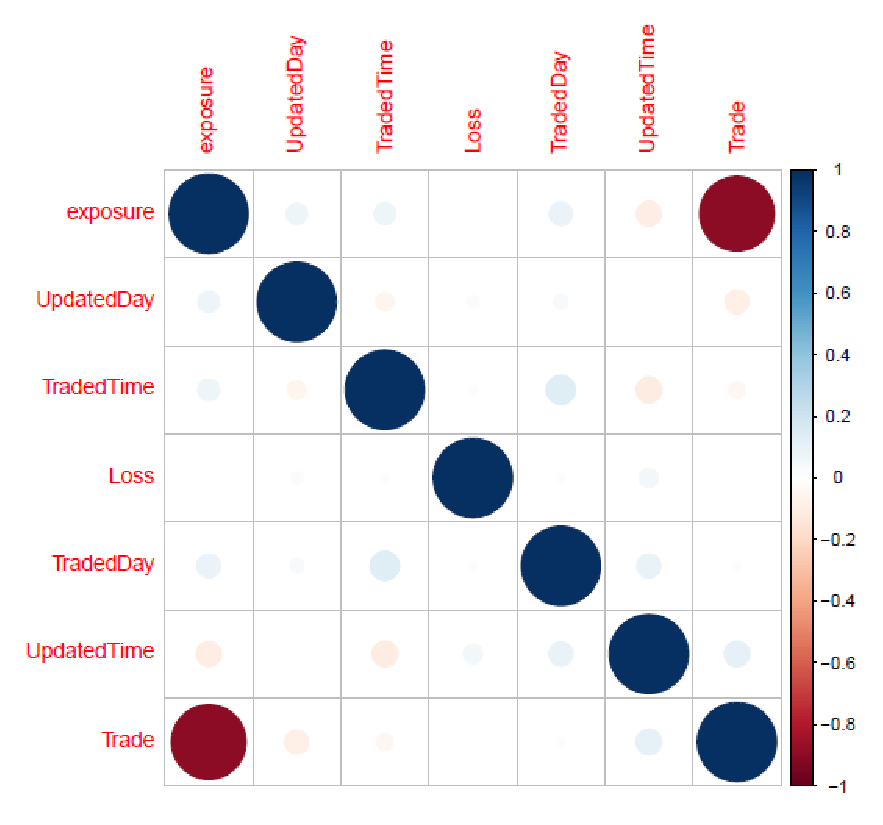
\includegraphics[width=7cm]{CorrPlot.eps}
         \end{tabular}
    \end{frame}
    \caption{Graphically displayed correlations by strength and a plot of OpRisk loss severities vs exposure}
    \label{Fig4}
\end{figure}

\subsection{The estimation of \emph{k}-means clustering algorithm}

A cluster analysis will identify groups within a dataset. The target
variable is LossIndicator, a binary variable indicating a \(1\) if a
realised loss occurs and \(0\) for those pending or near misses. The
\emph{K}-means clustering algorithm will search for K clusters
(specified by the user). The resulting \emph{k} clusters are represented
by the mean or average values of each of the variables. Let us consider
a model where the LossIndicator is the target variable: The user whose
task it is to specify \emph{k}, may guess right or in practice they may
obtain a priori, the knowledge of how to select the appropriate \emph{k}
in advance.\medskip

Rather than the trial and error method which involves guessing \emph{k}
values and successively computing minimum separation between centers,
there are several data mining techniques found in the literature, that
can be used to determine the optimal \emph{k} (Rousseeuw, 1987). The
output plot for the estimation of the optimal \emph{k} is presented in
Figure \ref{Fig5} below. We have iterated over cluster sizes from 2 to
10 clusters. The program KMeans resets the random number seed to obtain
the same results each time. where the optimal \emph{k} found to be
significant close to \(\emph{k} = 10\).\medskip

The plot displays the `sum(withinss)' for each clustering and the change
in this value from the previous clustering. The Sum(WithinSS) (blue
line) as a performance metric indicates that beyond \emph{k} = 4
clusters the model overfits: Its computes the absolute error which is
initially large, then monotonicaly decreases to the point \emph{k} = 4,
it then begins to increase subsequent to the point where the
Diffprevious Sum(WithinSS) (red line) intersects viz., at \emph{k} = 4
clusters, which means \emph{k} = 4 is the local optimal number of
clusters i.e., beyond which the iterative relative errors converges
faster than the absolute errors and successively reduces as \emph{k}
increases from 4 to 10.

\begin{figure}
\centering
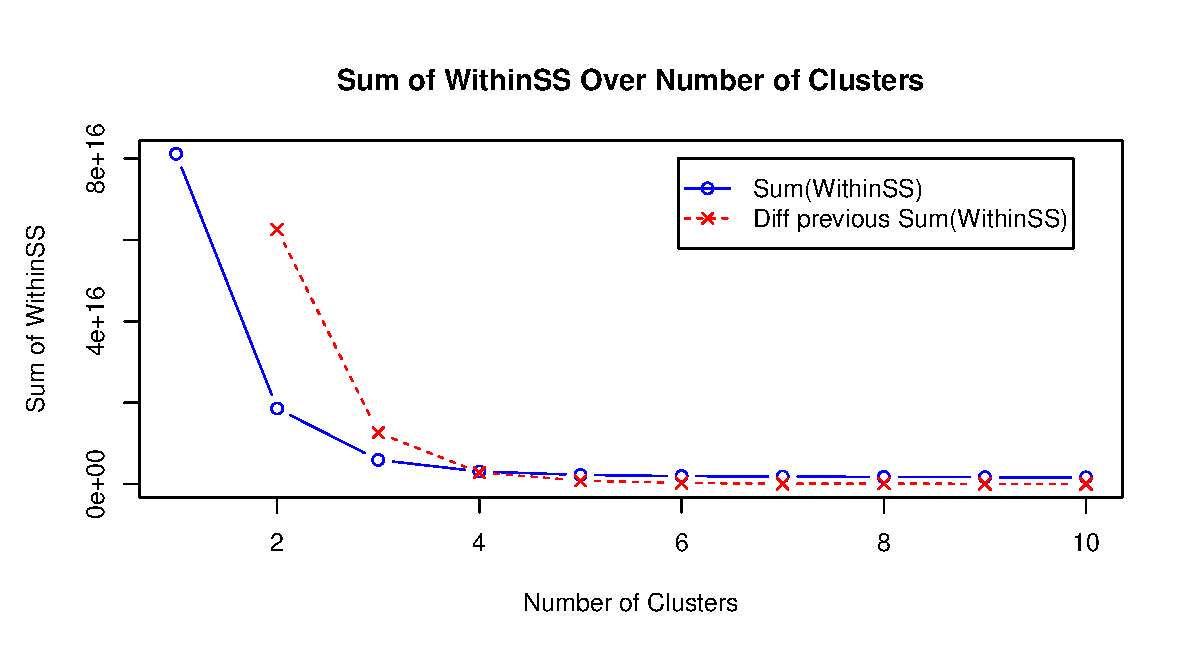
\includegraphics[width=15cm, height=7.5cm]{IterateKmeans.eps}
\caption{Finding the optimal number of \emph{k} groups by the Silhouette Statistic SS: Sum is a  measure to approximate the optimal number of \emph{k} groups by the Silhouette Statistic SS}
\label{IterateKmeans}
\end{figure}

\subsubsection{Rattle program code}

\subsubsection{Results}
\begin{verbatim}
Cluster sizes:

[1] "478 404 570 179"

Data means:

      Trade  UpdatedDay UpdatedTime   TradedDay  TradedTime 
0.762016409 0.448559166 0.486589314 0.487369712 0.601539912 
       Loss    exposure 
0.003232348 0.121083376 

Cluster centers:

      Trade UpdatedDay UpdatedTime TradedDay TradedTime        Loss
1 0.8106844  0.3943515   0.4123358 0.2912134  0.8556825 0.004692829
2 0.8716248  0.4900990   0.5409218 0.7948845  0.8270263 0.002132631
3 0.8378683  0.4493567   0.5264944 0.4160234  0.2165842 0.002308103
4 0.1431301  0.4970205   0.4351758 0.5443203  0.6397973 0.004757466
    exposure
1 0.08060460
2 0.06359981
3 0.07134609
4 0.51729829

Within cluster sum of squares:

[1]  84.88017  89.27845 148.89661  59.37208

Time taken: 1.86 secs

Rattle timestamp: 2018-12-13 07:22:48 User
\end{verbatim}

\begin{sidewaysfigure}
\centering
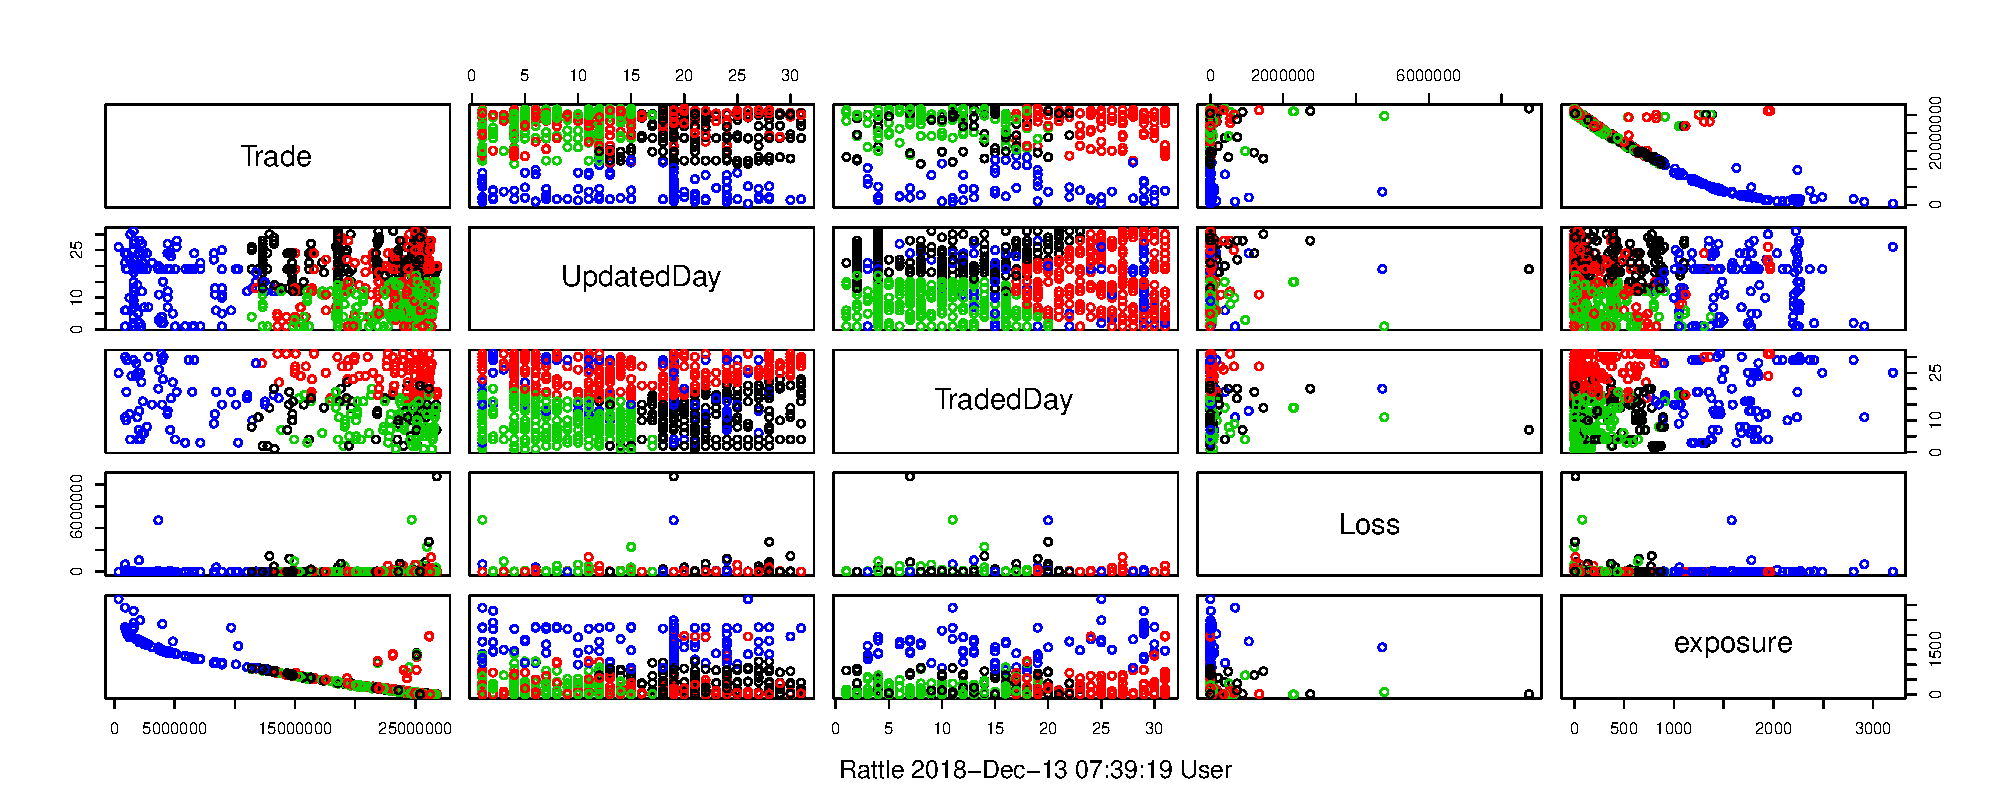
\includegraphics[width=22.5cm, height=15cm]{CA14MeansPlot.eps}
\caption{A scatterplot matrix for the \emph{k}-means clustering of size 4, and the covariates of frequency loss events consisting of 369 loss event frequencies amounting to R 61 534 745 P\&L severity of loss impact.}
\label{CA14MeansPlot}
\end{sidewaysfigure}

\singlespacing

\FloatBarrier
\newpage
\fancyhead[L]{References}
\fancyhead[R]{\thepage}
\fancyfoot[C]{}

\chapter*{REFERENCES}

\setlength{\parindent}{-0.5in}
\setlength{\leftskip}{0.4in}
\setlength{\parskip}{6pt}

\noindent

\hypertarget{refs}{}
\leavevmode\hypertarget{ref-acharyya2012current}{}%
Acharyya, M. (2012). Why the current practice of operational risk
management in insurance is fundamentally flawed: Evidence from the
field. \emph{ERM symposium, april}, 18--20.

\leavevmode\hypertarget{ref-agostini2010combining}{}%
Agostini, A., Talamo, P., \& Vecchione, V. (2010). Combining operational
loss data with expert opinions through advanced credibility theory.
\emph{The Journal of Operational Risk}, \emph{5}(1), 3.

\leavevmode\hypertarget{ref-aitkin1987modelling}{}%
Aitkin, M. (1987). Modelling variance heterogeneity in normal regression
using glim. \emph{Journal of the Royal Statistical Society: Series C
(Applied Statistics)}, \emph{36}(3), 332--339.

\leavevmode\hypertarget{ref-altman2008behavioral}{}%
Altman, M. (2008). \emph{Behavioral economics, economic theory and
public policy}.

\leavevmode\hypertarget{ref-aue2006lda}{}%
Aue, F., \& Kalkbrener, M. (2006). LDA at work: Deutsche bank's approach
to quantifying operational risk. \emph{Journal of Operational Risk},
\emph{1}(4), 49--93.

\leavevmode\hypertarget{ref-badescu2015modeling}{}%
Badescu, A. L., Lan, G., Lin, X. S., \& Tang, D. (2015). \emph{Modeling
correlated frequencies with application in operational risk management}.

\leavevmode\hypertarget{ref-barberis2003survey}{}%
Barberis, N., \& Thaler, R. (2003). A survey of behavioral finance.
\emph{Handbook of the Economics of Finance}, \emph{1}, 1053--1128.

\leavevmode\hypertarget{ref-boettrich2017recent}{}%
Boettrich, S., \& Starykh, S. (2017). Recent trends in securities class
action litigation: 2016 full-year review. \emph{NERA, New York}.

\leavevmode\hypertarget{ref-Burnham2002}{}%
Burnham, K. P., \& Anderson, D. R. (2002). \emph{Model selection and
multimodel inference: A practical information-theoretic approach}.
Springer-Verlag.

\leavevmode\hypertarget{ref-cameron2013regression}{}%
Cameron, A. C., \& Trivedi, P. K. (2013). \emph{Regression analysis of
count data} (Vol. 53). Cambridge university press.

\leavevmode\hypertarget{ref-chau2014robust}{}%
Chau, V. (2014). \emph{Robust estimation in operational risk modeling}
(Master's thesis).

\leavevmode\hypertarget{ref-chavez2016extreme}{}%
Chavez-Demoulin, V., Embrechts, P., \& Hofert, M. (2016). An extreme
value approach for modeling operational risk losses depending on
covariates. \emph{Journal of Risk and Insurance}, \emph{83}(3),
735--776.

\leavevmode\hypertarget{ref-chavez2006quantitative}{}%
Chavez-Demoulin, V., Embrechts, P., \& Nešlehová, J. (2006).
Quantitative models for operational risk: Extremes, dependence and
aggregation. \emph{Journal of Banking \& Finance}, \emph{30}(10),
2635--2658.

\leavevmode\hypertarget{ref-basel2010basel}{}%
Committee, B., \& others. (2010). Basel iii: A global regulatory
framework for more resilient banks and banking systems. \emph{Basel
Committee on Banking Supervision, Basel}.

\leavevmode\hypertarget{ref-basel2011operational}{}%
Committee, B., \& others. (2011). Operational risk--supervisory
guidelines for the advanced measurement approaches. \emph{Basel: Bank
for International Settlements}.

\leavevmode\hypertarget{ref-covrig2015using}{}%
Covrig, M., Mircea, I., Zbaganu, G., Coser, A., Tindeche, A., \& others.
(2015). Using r in generalized linear models. \emph{Romanian Statistical
Review}, \emph{63}(3), 33--45.

\leavevmode\hypertarget{ref-cruz2002modeling}{}%
Cruz, M. G. (2002). \emph{Modeling, measuring and hedging operational
risk}. John Wiley \& Sons New York,

\leavevmode\hypertarget{ref-de2008generalized}{}%
De Jong, P., \& Heller, G. Z. (2008). \emph{Generalized linear models
for insurance data}. Cambridge University Press.

\leavevmode\hypertarget{ref-denuit2007actuarial}{}%
Denuit, M., Maréchal, X., Pitrebois, S., \& Walhin, J.-F. (2007).
\emph{Actuarial modelling of claim counts: Risk classification,
credibility and bonus-malus systems}. John Wiley \& Sons.

\leavevmode\hypertarget{ref-dobson2008introduction}{}%
Dobson, A. J., \& Barnett, A. (2008). \emph{An introduction to
generalized linear models}. Chapman; Hall/CRC.

\leavevmode\hypertarget{ref-mysis2013}{}%
Dorval, M. (2013). \emph{Achieving Basel III compliance: how to tackle
it and business issues} (pp. 1--12). Retrieved from
\url{http://www.risktech-forum.com/research/achieving-basel-iii-compliance-how-to-tackle-it-and-business-issues}

\leavevmode\hypertarget{ref-einemann2018operational}{}%
Einemann, M., Fritscher, J., \& Kalkbrener, M. (2018). \emph{Operational
risk measurement beyond the loss distribution approach: An
exposure-based methodology}.

\leavevmode\hypertarget{ref-embrechts2018modeling}{}%
Embrechts, P., Mizgier, K. J., \& Chen, X. (2018). \emph{Modeling
operational risk depending on covariates. An empirical investigation.}

\leavevmode\hypertarget{ref-fahrmeir2013regression}{}%
Fahrmeir, L., Kneib, T., Lang, S., \& Marx, B. (2013). \emph{Regression:
Models, methods and applications}. Springer Science \& Business Media.

\leavevmode\hypertarget{ref-flake1998square}{}%
Flake, G. W. (1998). Square unit augmented radially extended multilayer
perceptrons. In \emph{Neural networks: Tricks of the trade} (pp.
145--163). Springer.

\leavevmode\hypertarget{ref-frachot2001loss}{}%
Frachot, A., Georges, P., \& Roncalli, T. (2001). \emph{Loss
distribution approach for operational risk}.

\leavevmode\hypertarget{ref-frees2010household}{}%
Frees, E. W., \& Sun, Y. (2010). Household life insurance demand: A
multivariate two-part model. \emph{North American Actuarial Journal},
\emph{14}(3), 338--354.

\leavevmode\hypertarget{ref-friedman1948utility}{}%
Friedman, M., \& Savage, L. J. (1948). The utility analysis of choices
involving risk. \emph{Journal of Political Economy}, \emph{56}(4),
279--304.

\leavevmode\hypertarget{ref-galloppo2014review}{}%
Galloppo, G., \& Previati, D. (2014). \emph{A review of methods for
combining internal and external data}.

\leavevmode\hypertarget{ref-gigerenzer2009homo}{}%
Gigerenzer, G., \& Brighton, H. (2009). Homo heuristicus: Why biased
minds make better inferences. \emph{Topics in Cognitive Science},
\emph{1}(1), 107--143.

\leavevmode\hypertarget{ref-gisiger2010risk}{}%
Gisiger, N. (2010). \emph{Risk-neutral probabilities explained}.

\leavevmode\hypertarget{ref-suntimes2019}{}%
Gous, N. (2019). \emph{Standard chartered pleads guilty to fixing the
rand} (pp. 1--2). Retrieved from
\url{https://www.timeslive.co.za/sunday-times/business/2019-02-05-standard-chartered-pleads-guilty-to-fixing-the-rand/}

\leavevmode\hypertarget{ref-ama2013ama}{}%
Group, A., \& others. (2013). AMA quantification challenges: AMAG range
of practice and observations on ``the thorny lda topics''. \emph{Munich:
Risk Management Association}.

\leavevmode\hypertarget{ref-harvey1976estimating}{}%
Harvey, A. C., \& others. (1976). Estimating regression models with
multiplicative heteroscedasticity. \emph{Econometrica}, \emph{44}(3),
461--465.

\leavevmode\hypertarget{ref-hemrit2012major}{}%
Hemrit, W., \& Arab, M. B. (2012). The major sources of operational risk
and the potential benefits of its management. \emph{The Journal of
Operational Risk}, \emph{7}(3), 71--92.

\leavevmode\hypertarget{ref-hoohlo2015new}{}%
Hoohlo, M. (2015). \emph{A new internal data measure for operational
risk: A case study of a south african bank} (PhD thesis).

\leavevmode\hypertarget{ref-de2015combining}{}%
Jongh, R. de, De Wet, T., Raubenheimer, H., \& Venter, J. H. (2015).
\emph{Combining scenario and historical data in the loss distribution
approach: A new procedure that incorporates measures of agreement
between scenarios and historical data}.

\leavevmode\hypertarget{ref-kahneman2003perspective}{}%
Kahneman, D. (2003). A perspective on judgment and choice: Mapping
bounded rationality. \emph{American Psychologist}, \emph{58}(9), 697.

\leavevmode\hypertarget{ref-kahneman2013prospect}{}%
Kahneman, D., \& Tversky, A. (2013). Prospect theory: An analysis of
decision under risk. In \emph{Handbook of the fundamentals of financial
decision making: Part i} (pp. 99--127). World Scientific.

\leavevmode\hypertarget{ref-orxablr2018}{}%
Kennett, R., \& Carrivick, L. (2018). \emph{Annual banking loss report:
operational risk loss data for banks submitted between 2012 and 2017}
(pp. 1--16). Retrieved from
\url{https://managingrisktogether.orx.org/orx-loss-data/annual-banking-loss-report}

\leavevmode\hypertarget{ref-king2001operational}{}%
King, J. L. (2001). \emph{Operational risk: Measurement and modelling
(the wiley finance series)}.

\leavevmode\hypertarget{ref-kneib2013beyond}{}%
Kneib, T. (2013). Beyond mean regression. \emph{Statistical Modelling},
\emph{13}(4), 275--303.

\leavevmode\hypertarget{ref-kuhnen2005neural}{}%
Kuhnen, C. M., \& Knutson, B. (2005). The neural basis of financial risk
taking. \emph{Neuron}, \emph{47}(5), 763--770.

\leavevmode\hypertarget{ref-list2004neoclassical}{}%
List, J. A. (2004). Neoclassical theory versus prospect theory: Evidence
from the marketplace. \emph{Econometrica}, \emph{72}(2), 615--625.

\leavevmode\hypertarget{ref-martin2009risk}{}%
Martin, P. H. (2009). As risk management evolves, is operational risk
management important? \emph{The Journal of Operational Risk},
\emph{4}(4), 75.

\leavevmode\hypertarget{ref-merton1974pricing}{}%
Merton, R. C. (1974). On the pricing of corporate debt: The risk
structure of interest rates. \emph{The Journal of Finance},
\emph{29}(2), 449--470.

\leavevmode\hypertarget{ref-mignola2016comments}{}%
Mignola, G., Ugoccioni, R., \& Cope, E. (2016). \emph{Comments on the
basel committee on banking supervision proposal for a new standardized
approach for operational risk}.

\leavevmode\hypertarget{ref-morgenstern1953theory}{}%
Morgenstern, O., \& Von Neumann, J. (1953). \emph{Theory of games and
economic behavior}. Princeton university press.

\leavevmode\hypertarget{ref-mori2001internal}{}%
Mori, T., Harada, E., \& others. (2001). \emph{Internal measurement
approach to operational risk capital charge}. Bank of Japan.

\leavevmode\hypertarget{ref-nelder1987extended}{}%
Nelder, J. A., \& Pregibon, D. (1987). An extended quasi-likelihood
function. \emph{Biometrika}, \emph{74}(2), 221--232.

\leavevmode\hypertarget{ref-nelder1972generalized}{}%
Nelder, J. A., \& Wedderburn, R. W. (1972). Generalized linear models.
\emph{Journal of the Royal Statistical Society: Series A (General)},
\emph{135}(3), 370--384.

\leavevmode\hypertarget{ref-ohlsson2010non}{}%
Ohlsson, E., \& Johansson, B. (2010). \emph{Non-life insurance pricing
with generalized linear models} (Vol. 2). Springer.

\leavevmode\hypertarget{ref-opdyke2014estimating}{}%
Opdyke, J. D. (2014). Estimating operational risk capital with greater
accuracy, precision, and robustness. \emph{arXiv Preprint
arXiv:1406.0389}.

\leavevmode\hypertarget{ref-panjer2006operational}{}%
Panjer, H. H. (2006). \emph{Operational risk: Modeling analytics} (Vol.
620). John Wiley \& Sons.

\leavevmode\hypertarget{ref-parodi2014pricing}{}%
Parodi, P. (2014). \emph{Pricing in general insurance}. CRC Press.

\leavevmode\hypertarget{ref-peters2016should}{}%
Peters, G., Shevchenko, P. V., Hassani, B., \& Chapelle, A. (2016).
\emph{Should the advanced measurement approach be replaced with the
standardized measurement approach for operational risk?}

\leavevmode\hypertarget{ref-rigby2017distributions}{}%
Rigby, R. A., Stasinopoulos, D., Heller, G. Z., \& De Bastiani, F.
(2017). Distributions for modelling location, scale, and shape: Using
gamlss in r. \emph{URL Www. Gamlss. Org.(last Accessed 5 March 2018)}.

\leavevmode\hypertarget{ref-risk2001supporting}{}%
Risk, B. O. (2001). Supporting document to the new basel capital accord.
\emph{Consultative Document, January}, \emph{200}.

\leavevmode\hypertarget{ref-risk2016supporting}{}%
Risk, B. O. (2016). Standardised measurement approach for operational
risk. \emph{Consultative Document, June}.

\leavevmode\hypertarget{ref-rosa2012litigation}{}%
Rosa, P. (2012). Litigation-credit risk structural models in op risk-an
exposure-based method using a credit risk structural model may help
operational risk managers predict underwriter litigations.
\emph{Operational Risk and Regulation}, \emph{13}(10), 34.

\leavevmode\hypertarget{ref-rousseeuw1987silhouettes}{}%
Rousseeuw, P. J. (1987). Silhouettes: A graphical aid to the
interpretation and validation of cluster analysis. \emph{Journal of
Computational and Applied Mathematics}, \emph{20}, 53--65.

\leavevmode\hypertarget{ref-shefrin2016behavioral}{}%
Shefrin, H. (2016). \emph{Behavioral risk management: Managing the
psychology that drives decisions and influences operational risk}.
Springer.

\leavevmode\hypertarget{ref-smyth1989generalized}{}%
Smyth, G. K. (1989). Generalized linear models with varying dispersion.
\emph{Journal of the Royal Statistical Society: Series B
(Methodological)}, \emph{51}(1), 47--60.

\leavevmode\hypertarget{ref-bustech2017}{}%
StaffWriter. (2017). \emph{Citibank to pay massive fine in SA currency
trading collusion scandal} (pp. 1--2). Retrieved from
\url{https://businesstech.co.za/news/banking/158931/citibank-to-pay-massive-fine-in-sa-currency-trading-collusion-scandal/}

\leavevmode\hypertarget{ref-stasinopoulos2018gamlss}{}%
Stasinopoulos, M. D., Rigby, R. A., \& Bastiani, F. D. (2018). GAMLSS: A
distributional regression approach. \emph{Statistical Modelling},
\emph{18}(3-4), 248--273.

\leavevmode\hypertarget{ref-stasinopoulos2017flexible}{}%
Stasinopoulos, M. D., Rigby, R. A., Heller, G. Z., Voudouris, V., \& De
Bastiani, F. (2017). \emph{Flexible regression and smoothing: Using
gamlss in r}. Chapman; Hall/CRC.

\leavevmode\hypertarget{ref-tom2007neural}{}%
Tom, S. M., Fox, C. R., Trepel, C., \& Poldrack, R. A. (2007). The
neural basis of loss aversion in decision-making under risk.
\emph{Science}, \emph{315}(5811), 515--518.

\leavevmode\hypertarget{ref-verbyla1993modelling}{}%
Verbyla, A. P. (1993). Modelling variance heterogeneity: Residual
maximum likelihood and diagnostics. \emph{Journal of the Royal
Statistical Society: Series B (Methodological)}, \emph{55}(2), 493--508.

\leavevmode\hypertarget{ref-voudouris2012modelling}{}%
Voudouris, V., Gilchrist, R., Rigby, R., Sedgwick, J., \& Stasinopoulos,
D. (2012). Modelling skewness and kurtosis with the bcpe density in
gamlss. \emph{Journal of Applied Statistics}, \emph{39}(6), 1279--1293.

\leavevmode\hypertarget{ref-williams2011data}{}%
Williams, G. (2011). \emph{Data mining with rattle and r: The art of
excavating data for knowledge discovery}. Springer Science \& Business
Media.

\leavevmode\hypertarget{ref-wiseman1997longitudinal}{}%
Wiseman, R. M., \& Catanach Jr, C. (1997). A longitudinal disaggregation
of operational risk under changing regulations: Evidence from the
savings and loan industry. \emph{Academy of Management Journal},
\emph{40}(4), 799--830.

\leavevmode\hypertarget{ref-wood2017generalized}{}%
Wood, S. N. (2017). \emph{Generalized additive models: An introduction
with r}. Chapman; Hall/CRC.

\leavevmode\hypertarget{ref-yan2009applications}{}%
Yan, J., Guszcza, J., Flynn, M., \& Wu, C.-S. P. (2009). Applications of
the offset in property-casualty predictive modeling. \emph{Casualty
actuarial society e-forum, winter 2009}, 366.

\clearpage
\addcontentsline{toc}{chapter}{APPENDICES}
\fancyhead[L]{Appendices}
\fancyhead[R]{\thepage}
\fancyfoot[C]{}

\vspace*{\fill}
  \begin{center}
    APPENDICES 
  \end{center}
\vspace*{\fill}

\clearpage

\doublespacing

\section{Appendix A: R Code and Data Preparation for Chapter 3}
\label{sec:Appendix A: R Code and Data Preparation for Chapter 3}

\singlespace

Required: R Packages from CRAN

\small

\begin{verbatim}
if (!require(caTools)){
  install.packages("caTools")
  library(caTools)
}
if (!require(caret)){
  install.packages("caret")
  library(caret)
}
if (!require(R2HTML)){
  install.packages("R2HTML")
  library(R2HTML)
}
if (!require(rattle)){
  install.packages("rattle")
  library(rattle)
}
if (!require(magrittr)){
  install.packages("magrittr")
  library(magrittr)
}
if (!require(dplyr)){
  install.packages("dplyr")
  library(dplyr)
}
if (!require(Hmisc)){
  install.packages("Hmisc")
  library(Hmisc)
}
if (!require(chron)){
  install.packages("chron")
  library(chron)
}  
  if (!require(ggplot2)){
  install.packages("ggplot2")
  library(ggplot2)
  }
\end{verbatim}

\normalsize

\subsection{Data preparation for understanding the raw frequency and raw severity data mentioned in
section \ref{sec:Exploratory data analysis} on page \pageref{sec:Exploratory data analysis} of collected internally over the period
between 1 January 2013 and 31 March 2013 i.e., Q12013 at an investment bank in SA}
\label{ssec:Data preparation raw}

\small

\begin{verbatim}
file_loc <- "C:/Users/Mphekeleli/Documents/R PROJECT/OpRiskPHDGitHub
/OpRisk_PHD_Thesis/Data"
setwd(file_loc)
list.files(file_loc)
frequency <- openxlsx::read.xlsx("Raw_Formatted_Data.xlsx",
                      check.names = TRUE, sheet = "Frequency")
severity <- openxlsx::read.xlsx("Raw_Formatted_Data.xlsx",
                      check.names = TRUE, sheet = "Severity")
projdata <- openxlsx::read.xlsx("OPriskDataSet_exposure.xlsx",
                      check.names = TRUE, sheet = "CleanedData")
\end{verbatim}

\normalsize

\subsection{Data preparation providing the numbers of OpRisk events collected through pre-processing by following the LCDE as described in section \ref{sec:Description of the dataset} on \pageref{sec:Description of the dataset} over Q12013, limited to the covariates selected to fit into the models}
\label{ssec:Data preparation pre-processed}

\small

\begin{verbatim}
# Set parameter values
crv$seed <- 42 # set random seed
crv$training.proportion <- 1.0

# Load data
fname <- "file:///G:/PHD/OPRISK_PHD_DISS/Data/OPriskDataSet_exposure.csv"
crs$dataset <- read.csv(fname,
              sep=";",
              dec=",",
              na.strings=c(".", "NA", "", "?"),
              strip.white=TRUE, encoding="UTF-8")

# Build the train/validate/test datasets.

# nobs=2330 train=2330 validate=0 test=0
set.seed(crv$seed)
crs$nobs   <- nrow(crs$dataset)
crs$sample <- sample(crs$nobs, crv$training.proportion * crs$nobs)
crs$train  <- crs$sample <- sample(crs$nobs, crv$training.proportion * crs$nobs)
# crs$train  <- sample(crs$nobs, 1*crs$nobs)
crs$validate <- NULL
crs$test <- NULL

# The following variable selections have been noted.
crs$input     <- c("Trade", "UpdatedDay", "UpdatedTime",
                   "TradedDay", "TradedTime", "Desk", "CapturedBy",
                   "TradeStatus", "TraderId", "Instrument", "Reason",
                   "Loss", "EventTypeCategoryLevel1",
                   "BusinessLineLevel1", "exposure")

crs$numeric   <- c("Trade", "UpdatedDay", "UpdatedTime",
                   "TradedDay", "TradedTime", "Loss", "exposure")

crs$categoric <- c("Desk", "CapturedBy", "TradeStatus",
                   "TraderId", "Instrument", "Reason",
                   "EventTypeCategoryLevel1", "BusinessLineLevel1")

crs$target    <- "LossIndicator"
crs$risk      <- NULL
crs$ident     <- NULL
crs$ignore    <- c("UpdateTime", "TradeTime", "Nominal", "FloatRef", 
                   "LastResetDate", "LastResetRate", "Theta", "Unexplained")
crs$weights   <- NULL
\end{verbatim}

\normalsize

\subsection{The algorithm only accepts numerical data and so categorical data is transformed into numeric. This is done using an approach where each value of a categoric variable is turned into a variable itself. Multi-level categoric variables are recoded by building dummy variables corresponding to each level by the following commands:}
\label{ssec:Transforming to dummy variables}

Numerical and categoric variables (to be transformed by below conversion
code) depicted in table \ref{tab_contents} on page
\pageref{tab_contents}:

\small

\begin{verbatim}
# Remap factor variables and transform into numeric variables.
crs$dataset[["TNM_Desk"]] <- as.numeric(crs$dataset[["Desk"]])
crs$dataset[["TNM_CapturedBy"]] <- as.numeric(crs$dataset[["CapturedBy"]])
crs$dataset[["TNM_TraderId"]] <- as.numeric(crs$dataset[["TraderId"]])
crs$dataset[["TNM_Instrument"]] <- as.numeric(crs$dataset[["Instrument"]])
crs$dataset[["TNM_Reason"]] <- as.numeric(crs$dataset[["Reason"]])
crs$dataset[["TNM_EventTypeCategoryLevel1"]] <- as.numeric(crs$dataset
                                        [["EventTypeCategoryLevel1"]])
crs$dataset[["TNM_BusinessLineLevel1"]] <- as.numeric(crs$dataset
                                             [["BusinessLineLevel1"]])
\end{verbatim}

\normalsize

\subsection{Scatterplots and Histograms plots of loss severities and frequency counts against selected explanatory variables showing basic
summary statistics of intra-day trading activity}
\label{ssec:Scatterplots and Histograms of intra-day trading activity}

Figures \ref{Intra_Day_Trends} and \ref{Hist_Loss_Freq} on page
\pageref{Hist_Loss_Freq}:

\small

\begin{verbatim}
# Scatterplots for loss severities
plot(projdata$UpdatedTime, log(projdata$Loss+0.000000001), ylim = c(6, 18),
     col = "navy", xlab = "Updated Time", ylab = "Log. Loss")
xyplot(Loss ~ as.factor(TraderId) , data = projdata)

# Histograms for loss severities
hist(projdata$UpdatedDay, col = "#9999CC", main = "All losses", xlab = "Updated Day"
     , ylab = "Frequency")
hist(projdata$TradedDay)
\end{verbatim}

\normalsize

\subsection{Characteristics of exposure: Exposure data is used for several of the steps of the process in frequency and severity modelling}
\label{ssec:Characteristics of exposure}

Figure \ref{Exploration_analysis_exposure} on page
\pageref{Exploration_analysis_exposure}:

\small

\begin{verbatim}
#######Display histogram plots for the selected variables##########
#============================================================
# Display histogram plots for the selected variables. Use ggplot2 to generate
# histogram plot for exposure. Generate the plot.

Exp <- crs %>%
  with(dataset[train,]) %>%
  dplyr::select(exposure) %>%
  ggplot2::ggplot(ggplot2::aes(x=exposure)) +
  ggplot2::geom_density(lty=1, lwd=1) +
  ggplot2::geom_density(ggplot2::aes(fill="", colour=""), alpha=0.55) +
  ggplot2::xlab("Exposure") +
  ggplot2::ggtitle("Pdf(exposure)") +
  ggplot2::labs(y="Density") +
  theme_bw(base_size = 15) +
  theme(legend.position = "none")

# Display the plots.
gridExtra::grid.arrange(Exp)

#============================================================
# Generate just the data for an Ecdf plot of the variable 'exposure'.
ds <- rbind(data.frame(dat=crs$dataset[crs$train,][,"exposure"], grp="All"))

# The 'Hmisc' package provides the 'Ecdf' function.
library(Hmisc, quietly=TRUE)

# Plot the data.
Ecdf(ds[ds$grp=="All",1], col="red", xlab="exposure", lwd=2, 
     ylab=expression(Proportion <= x), subtitles=FALSE)

# Add a title to the plot.
title(main="Cdf(exposure)")
    
#============================================================
# Benford's Law 

# The 'ggplot2' package provides the 'ggplot' function.
library(ggplot2, quietly=TRUE)

# The 'reshape' package provides the 'melt' function.
library(reshape, quietly=TRUE)

# Initialies the parameters.
var    <- "exposure"
digit  <- 1
len    <- 1

# Build the dataset
ds <- merge(benfordDistr(digit, len),
            digitDistr(crs$dataset[crs$train,][var], digit, len, "All"))

# Plot the digital distribution
p <- plotDigitFreq(ds)
p <- p + ggtitle("Digital Analysis") +
  theme(
    legend.position = c(.95, .95),
    legend.justification = c("right", "top"),
    legend.box.just = "right",
    legend.margin = margin(6, 6, 6, 6)
    ) +
  # custom box around legend
 theme(
    legend.box.background = element_rect(color="red", size=2),
    legend.box.margin = margin(6, 6, 6, 6)
) +
# custom the key
 theme(legend.key = element_rect(fill = "white", colour = "black")) +
# custom the text
 theme(legend.text = element_text(size = 8, colour = "red")) +
# custom the title
 theme(legend.title = element_text(face = "bold"))
print(p)
# #============================================================
\end{verbatim}

\normalsize

\subsection{Histograms for frequency characteristics of daily and monthly operations for daily losses and/or pending/near misses}
\label{ssec:Frequency characteristics of operational activity}

Figures \ref{Exploratory_UpdateTime_Frequency3plot} and
\ref{Exploratory_UpdateDay_Frequency3plot} on page
\pageref{Exploratory_UpdateTime_Frequency3plot}:

\small

\begin{verbatim}
################   EXPLORATORY DATA ANALYSIS  ###################
#___________________________________________________________________________________________________
# Update Time
### summary statistics
 summary(projdata$UpdatedTime)

### Histograms - ALL Losses and Near Misses/Pending Losses and Realised losses 
par(mfrow=c(1,3))
hist(projdata$UpdatedTime, col = "blue", main = "All losses", 
     xlab = "Update Time", ylab = "Frequency")
hist(projdata$UpdatedTime[projdata$LossIndicator == 0], col = "red",
     main = "Near Misses", xlab = "Update Time", ylab = "Frequency")
hist(projdata$UpdatedTime[projdata$LossIndicator == 1], col = "green",
     main = "Realised losses", xlab = "Update Time", ylab = "Frequency")
par(mfrow=c(1,1))
#___________________________________________________________________________________________________
# # Update Day
 summary(projdata$UpdatedDay)

### Histograms - ALL Losses and Near Misses/Pending Losses and Realised losses
par(mfrow=c(1,3))
hist(projdata$UpdatedDay, col = "#9999CC", main = "All losses",
     xlab = "Updated Day", ylab = "Frequency")
hist(projdata$UpdatedDay[projdata$LossIndicator == 0], col = "#CC6666",
     main = "Near Misses", xlab = "Updated Day", ylab = "Frequency")
hist(projdata$UpdatedDay[projdata$LossIndicator == 1], col = "#66CC99",
     main = "Realised losses", xlab = "Updated Day", ylab = "Frequency")
par(mfrow=c(1,1))
\end{verbatim}

\normalsize

\subsection{Density plots of overlaid trade proportions of realised losses vs pending losses/near misses}
\label{ssec:Density plots}

Figures \ref{Density_Proportions} on page \pageref{Density_Proportions}:

\small

\begin{verbatim}
# Density Plot for Updated Day
p01 <- crs %>%
  with(dataset[sample,]) %>%
  dplyr::mutate(LossIndicator=as.factor(LossIndicator)) %>%
  dplyr::select(UpdatedDay, LossIndicator) %>%
  ggplot2::ggplot(ggplot2::aes(x=UpdatedDay)) +
  ggplot2::geom_density(lty=3) +
  ggplot2::geom_density(ggplot2::aes(fill=LossIndicator, colour=LossIndicator)
                        , alpha=0.55) +
  ggplot2::ggtitle("Distr. of Updated DaY") +
  ggplot2::labs(fill="LossIndicator", y="Density") +
  ggplot2::xlab("Day of Month that Trade Was Updated") +
  ggplot2::theme(legend.position=c(.7,.2))

# Density Plot for Traded day
p02 <- crs %>%
  with(dataset[sample,]) %>%
  dplyr::mutate(LossIndicator=as.factor(LossIndicator)) %>%
  dplyr::select(TradedDay, LossIndicator) %>%
  ggplot2::ggplot(ggplot2::aes(x=TradedDay)) +
  ggplot2::geom_density(lty=3) +
  ggplot2::geom_density(ggplot2::aes(fill=LossIndicator, colour=LossIndicator)
                        , alpha=0.55) +
  ggplot2::ggtitle("Distr. of TradedDay") +
  ggplot2::labs(fill="LossIndicator", y="Density") +
  ggplot2::xlab("Day of Month for Trade") +
  ggplot2::theme(legend.position=c(.7,.2))

# Display the plots.
gridExtra::grid.arrange(p01, p02, nrow = 1)
\end{verbatim}

\normalsize

Table \ref{tab_Desk_Prop} on \pageref{tab_Desk_Prop}

\small

\begin{verbatim}
# addmargins(table(projdata$Desk, projdata$LossIndicator), 2)
\end{verbatim}

\normalsize

\subsection{Histograms of overlaid trade proportions of realised losses vs pending loss/near misses}
\label{ssec:Histogram proportions}

Figures \ref{Desk_Proportions} on page \pageref{Desk_Proportions}:

\small

\begin{verbatim}
# Plot Desk category distribution
p03 <- crs %>%
  with(dataset[sample,]) %>%
  dplyr::mutate(LossIndicator=as.factor(LossIndicator)) %>%
  dplyr::select(Desk, LossIndicator) %>%
  dplyr::group_by(Desk, LossIndicator) %>%
  dplyr::summarise(n = n()) %>%
  ggplot2::ggplot(ggplot2::aes(x=Desk, y=n, fill=LossIndicator)) +
  ggplot2::geom_bar(stat="identity") +
  ggplot2::ggtitle("Desk category distribution") +
  ggplot2::theme_minimal() +
  ggplot2::theme(axis.text.x = element_text(angle = 90, hjust = 1))+
  ggplot2::ylab("Frequency")

# Create new variable to proportion no. of realised losses
T01 <- crs %>%
  with(dataset[sample,]) %>%
  dplyr::mutate(LossIndicator=as.factor(LossIndicator)) %>%
  dplyr::select(Desk, LossIndicator) %>%
  dplyr::group_by(Desk, LossIndicator) %>%
  dplyr::summarise(n = n())

T02 <- T01 %>%
  group_by(Desk) %>%
  summarise(N=sum(n))

T03 <- inner_join(T01, T02)

# Plot Desk category by proportion
T04 <- T03 %>%
  mutate(Prob=n/N) %>%
  filter(LossIndicator==1) %>%
  select(Desk, Prob) %>%
  arrange(desc(Prob)) %>%
  ggplot2::ggplot(ggplot2::aes(x=Desk, y=Prob, fill=Desk), alpha=0.55) +
  ggplot2::geom_bar(stat="identity", fill="grey", colour="black", show.legend = FALSE)+
  ggplot2::ggtitle("Proportion of losses per Desk") +
  ggplot2::theme_minimal()+
  ggplot2::theme(axis.text.x = element_text(angle = 90, hjust = 1))+
  ggplot2::ylab("Loss Ratio (n/N)")+
  ggplot2::xlab("Desk")

#Display both plots in one row
gridExtra::grid.arrange(p03, T04, nrow = 1)
####============================================================
\end{verbatim}

\normalsize

\subsection{Mosaic grid plots for the bidimensional distributions by traded \texttt{Instrument}, \texttt{TraderId} and number}
\label{ssec:Mosaic bidimensional grid plot}

Figures \ref{Mosaic_Instr_Trd_Tec} on page
\pageref{Mosaic_Instr_Trd_Tec}:

\small

\begin{verbatim}
par(mfrow=c(1,2))
plot(table(projdata$LossIndicator, projdata$Instrument), main="By Instrument",
     col=rainbow(20), las=1)
plot(table(projdata$LossIndicator, projdata$TraderId), main="By Trader", 
     col=rainbow(20), las=1)
plot(table(projdata$LossIndicator, projdata$CapturedBy), main="By Tech Support",
     col=rainbow(20), las=1)
par(mfrow = c(1, 1))
####============================================================
\end{verbatim}

\normalsize

\subsection{Mosaic grid plots for the structure of OpRisk portfolio by traded \texttt{TradeStatus}, \texttt{TraderId} by the number of realised losses vs pending loss/near misses}
\label{ssec:Mosaic cross-sectional plot}

Figures \ref{Mosaic_Instr_Trd_Tec} on page
\pageref{Mosaic_Instr_Trd_Tec}:

\small

\begin{verbatim}
# Contingency Table
library(vcd)
STD <- structable(~TradeStatus + TraderId + LossIndicator, data = projdata)
par(cex.axis = 1.5, cex.lab = 0.1)
# Mosaic plot
MS01 <- mosaic(STD, condvars = 'TradeStatus', col=rainbow(20), 
      split_horizontal = c(TRUE, FALSE, TRUE), shade = TRUE, legend = TRUE)
MS01
\end{verbatim}

\normalsize

\clearpage

\section{Appendix B: R Code for Chapter 4}
\label{sec:Appendix B: R Code for Chapter 4}

\singlespace

Required: R Packages from CRAN (in addition to packages already found in
Chapter 3)

\small

\begin{verbatim}
if (!require(MuMIn)){
  install.packages("MuMIn")
  library(MuMIn)
}
if (!require(parallel)){
  install.packages("parallel")
  library(parallel)
}
if (!require(R2HTML)){
  install.packages("R2HTML")
  library(R2HTML)
}
if (!require(e1071)){
  install.packages("e1071")
  library(e1071)
}
if (!require(ROCR)){
  install.packages("ROCR")
  library(ROCR)
}
\end{verbatim}

\normalsize

\subsection{Data partitioning of the pre-processed OpRisk dataset into Training/Validation/Testing proportions, in preparation for machine learning model building treatments. The original dataset is partitioned into three random subsets initiated by a random number sequence with a randomly selected seed.}
\label{ssec:Data Training/Validation/Testing}

The function \texttt{getmode} specifies the modal class as the reference
level in the GLM from which the corresponding observations are estmated
and weighted against, see chapter
\ref{DATA EXPLORATION AND EXPOSURE VARIABLE ANALYSIS} section
\ref{sec:Exploratory data analysis} on page
\pageref{sec:Exploratory data analysis}

\small

\begin{verbatim}
building <- TRUE
scoring <- ! building

# Load data
fname <- "file:///C:/Users/Mphekeleli/Documents/R PROJECT/OpRiskPHDGitHub
/OpRisk_PHD_Thesis/Data/OPriskDataSet_exposure.csv"
crs$dataset <- read.csv(fname,
              sep=";",
              dec=",",
              na.strings=c(".", "NA", "", "?"),
              strip.white=TRUE, encoding="UTF-8")
exposure <- crs$dataset[,ncol(crs$dataset)]

# Select variables for loss incident model
crs$dataset <- as.data.frame(crs$dataset)

# The following varaible selections have been noted

crs$input <- crs$dataset %>%
  group_by(UpdatedDay,
           UpdatedTime,
           TradedDay,
           TradedTime,
           Desk,
           CapturedBy,
           TradeStatus,
           TraderId,
           Instrument,
           Reason,
           EventTypeCategoryLevel1,
           BusinessLineLevel1) %>%
  transmute(LossesIndicator = LossIndicator,
            Losses = Loss,
            Exposure = exposure)

getmode <- function(x){
  u <- unique(x)
  as.integer(u[which.max(tabulate(match(x,u)))])
}

for (i in 5:(ncol(crs$input) - 3)){
     crs$input[[i]] <- relevel(crs$input[[i]], getmode(crs$input[[i]]))
}

#==========================================================================================
# A predefined value is used to reset the random seed so that results are repeatable
crv$seed <- 42 

# Build the training/validation/testing datasets. Set parameter values
   

set.seed(crv$seed)    # set random seed to make your partition reproducible

crs$nobs <- nrow(crs$input)                 # nobs=2331

crs$train <- sample(crs$nobs, 0.7*crs$nobs) # proportion of training data = 1632 

crs$nobs %>%
  seq_len() %>%
  setdiff(crs$train) %>%
  sample(0.15*crs$nobs) ->                  # proportion of validation data = 350 
  crs$validate

crs$nobs %>%
  seq_len() %>%
  setdiff(crs$train) %>%
  setdiff(crs$validate) ->                  # proportion of testing data = 349 
  crs$test


crs$training <- as.data.frame(crs$input[crs$train,])
crs$validation <- as.data.frame(crs$input[crs$validate,])
crs$testing <- as.data.frame(crs$input[crs$test,])
\end{verbatim}

\normalsize

\doublespacing

\section{Models}
\label{sec:Models}

\singlespace

\subsection{Estimation of some poisson regression models for OpRisk loss frequency distribution: To build the model we pass on to the model building function \texttt{glm} i.e., the formula that describes the model to build.}
\label{ssec:Estimation of some poisson regression models for OpRisk loss frequency distribution}

use ``LossesIndicator'' as the dependent variable, \texttt{TradedDay}
and \texttt{Desk} variables are predictor variables.

\small

\normalsize

\emph{Basic model build summary}

\begin{verbatim}
Call:
glm(formula = LossesIndicator ~ TradedDay + Desk, family = poisson(link = "log"), 
    data = crs$training, offset = log(Exposure))

Deviance Residuals: 
    Min       1Q   Median       3Q      Max  
-2.8706  -0.5300  -0.2286  -0.0545   4.3750  

Coefficients:
                      Estimate Std. Error z value             Pr(>|z|)    
(Intercept)          -8.053221   0.193632 -41.590 < 0.0000000000000002 ***
TradedDay            -0.014087   0.006381  -2.208             0.027266 *  
DeskAfrica            1.457695   0.413087   3.529             0.000417 ***
DeskBonds/Repos       1.764230   0.254571   6.930      0.0000000000042 ***
DeskCommodities       0.924033   0.235749   3.920      0.0000887114575 ***
DeskDerivatives      -0.577626   0.344672  -1.676             0.093763 .  
DeskEquity            1.365152   0.225948   6.042      0.0000000015232 ***
DeskManagement/Other -1.410706   1.014052  -1.391             0.164177    
DeskMM                0.339561   0.241501   1.406             0.159711    
DeskPrime Services    2.129594   0.223030   9.548 < 0.0000000000000002 ***
DeskSND              -0.716361   0.283796  -2.524             0.011596 *  
---
Signif. codes:  0 ‘***’ 0.001 ‘**’ 0.01 ‘*’ 0.05 ‘.’ 0.1 ‘ ’ 1

(Dispersion parameter for poisson family taken to be 1)

    Null deviance: 1994.9  on 1630  degrees of freedom
Residual deviance: 1764.7  on 1620  degrees of freedom
AIC: 2310.7

Number of Fisher Scoring iterations: 8
\end{verbatim}

\subsection{Let us now fit a broader GLM to be our global model, still \texttt{LossesIndicator} as the dependent variable, while the rest of the predictive variables will be predictor variables.}
\label{ssec:GLM estimation results}

\small

\begin{verbatim}
freqfit <- glm(formula = LossesIndicator ~ UpdatedDay + UpdatedTime + TradedDay + 
    TradedTime + Desk + CapturedBy + TradeStatus + TraderId + 
    Instrument + Reason + EventTypeCategoryLevel1 + BusinessLineLevel1, 
    family = poisson(link = "log"), data = crs$training, 
    offset = log(Exposure)))
\end{verbatim}

\normalsize

\emph{Global model build summary}

\begin{verbatim}

Call:
glm(formula = LossesIndicator ~ UpdatedDay + UpdatedTime + TradedDay + 
    TradedTime + Desk + CapturedBy + TradeStatus + TraderId + 
    Instrument + Reason + EventTypeCategoryLevel1 + BusinessLineLevel1, 
    family = poisson(link = "log"), data = crs$training, 
    offset = log(Exposure))

Deviance Residuals: 
    Min       1Q   Median       3Q      Max  
-4.7605  -0.3575  -0.1105  -0.0315   3.9754  

Deviance Residuals: 
    Min       1Q   Median       3Q      Max  
-4.7605  -0.3575  -0.1105  -0.0315   3.9754  

Coefficients:
                       Estimate     Std. Error z value             Pr(>|z|)    
(Intercept)           -7.8113982    0.6701090 -11.657 < 0.0000000000000002 ***
UpdatedDay             0.0043298    0.0097374   0.445             0.656565    
UpdatedTime            0.5850748    0.7146037   0.819             0.412935    
TradedDay             -0.0001216    0.0082899  -0.015             0.988297    
TradedTime            -0.8201083    0.7856849  -1.044             0.296572    
DeskAfrica             1.5831846    0.5281939   2.997             0.002723 ** 
DeskBonds/Repos        2.3432611    0.3958404   5.920     0.00000000322505 ***
DeskCommodities        0.6910019    0.4627163   1.493             0.135343    
DeskDerivatives        0.3832286    0.5020354   0.763             0.445255    
DeskEquity             1.1778919    0.3969116   2.968             0.003001 ** 
DeskManagement/Other -14.7535497  367.5957685  -0.040             0.967985    
DeskMM                 1.2027479    0.5903580   2.037             0.041618 *  
DeskPrime Services    -0.1311216    1.3579826  -0.097             0.923079    
DeskSND                0.0518179    0.7105464   0.073             0.941864    
CapturedByMIDOFFICE    0.2618294    0.3319433   0.789             0.430242    
CapturedByPROD ACCOUN
TANT                   0.0934629    0.5393415   0.173             0.862423    
CapturedByPROD 
CONTROLLER            -0.4702595    0.3321428  -1.416             0.156824    
CapturedByUNAUTHORISED-0.9738648    0.5370115  -1.813             0.069756 .  
TradeStatusBO-BO 
Confirmed             -0.3379764    0.2363953  -1.430             0.152801    
TradeStatusTerminated  2.1847205    1.3465905   1.622             0.104716    
TradeStatusTerminated
/Void                 11.3395140 1443.2959040  -0.008             0.993731    
TraderIdAMBA           0.4943858    0.5830511   0.848             0.396478    
TraderIdANALYST       -0.2062667    0.2944408  -0.701             0.483592    
TraderIdASSOCIATE     -0.7844915    0.3507247  -2.237             0.025301 *  
TraderIdATS            2.7382867    0.6662928   4.110     0.00003961139187 ***
TraderIdMNGDIRECTOR    0.6153055    0.3144102   1.957             0.050346 .  
TraderIdVICE PRINCIPAL 0.2229076    0.3662304   0.609             0.542754    
InstrumentBill         0.7859508    0.6781491   1.159             0.246471    
InstrumentBond        -0.3433677    0.4080143  -0.842             0.400035    
InstrumentBuySellback  0.1566566    0.6720075   0.233             0.815670    
InstrumentCall Deposit-1.2603996    0.3973057  -3.172             0.001512 ** 
InstrumentCombination  0.6328848    1.2513624   0.506             0.613028    
InstrumentCredit
DefaultSwap           -1.9878550    0.6529647  -3.044             0.002332 ** 
InstrumentCurr        -1.0355350    0.5045561  -2.052             0.040134 *  
InstrumentCurrSwap    -0.6964712    0.5165406  -1.348             0.177550    
InstrumentDeposit      0.0584655    0.3945317   0.148             0.882193    
InstrumentEquityIndex -0.8243925    1.0794767  -0.764             0.445048    
InstrumentETF          1.0751791    1.1397155   0.943             0.345489    
InstrumentFRA         -1.6745203    0.9177750  -1.825             0.068070 .  
InstrumentFRN          0.2792480    0.5903548   0.473             0.636201    
InstrumentFuture/
Forward               -0.7303512    0.3917942  -1.864             0.062305 .  
InstrumentIndexLinked
Bond                  -0.6022619    0.7595690  -0.793             0.427836    
InstrumentIndexLinked
Swap                  -0.0154039    0.6024804  -0.026             0.979602    
InstrumentOption       0.0277106    0.5621959   0.049             0.960688    
InstrumentOther       -0.1830206    0.2891929  -0.633             0.526821    
InstrumentRepo/Reverse-2.0252367    0.7133321  -2.839             0.004524 ** 
InstrumentSecurityLoan-1.0447821    0.3461497  -3.018             0.002542 ** 
InstrumentStock       -0.6782734    1.4169911  -0.479             0.632172    
InstrumentTotalReturn
Swap                  -1.0219974    0.3990992  -2.561             0.010444 *  
ReasonAcquirer         4.2877314    1.2671128   3.384             0.000715 ***
ReasonBrokerage 
Related                1.7788236    1.0318752   1.724             0.084730 .  
ReasonCalendar Related 1.2768935    0.3888510   3.284             0.001024 ** 
ReasonCapture Errors    
Direct/Amount/Rate/CP  0.2418004    0.4150033   0.583             0.560131  
ReasonClient Request
to Amend Economics of
Deal              -0.9290734    1.0584940  -0.878             0.380089   
ReasonCommodities
Early Delivery        -0.4631230    1.2048262  -0.384             0.700689    
ReasonCorrected 
NDEUSSA Reset Level   -2.8475291    0.8317484  -3.424             0.000618 ***
ReasonCPI Fixings     -4.2562507    0.9924649  -4.289     0.00001798306834 ***
ReasonEarly Terminati
on/Delivery/ Close out-2.6225044    0.7518160  -3.488             0.000486 ***
ReasonFees/Commissions
Related               -1.4712607    0.9402884  -1.565             0.117655    
ReasonOperations 
request to change 
Economics of Trade    -0.1702668    0.8638805  -0.197             0.843753    
ReasonPayments Related-0.5039834    0.7179092  -0.702             0.482669    
ReasonPortfolio Move
 / Restructure        -1.8408735    1.1353256  -1.621             0.104921    
ReasonSales Credits    2.1487308    1.1446783   1.877             0.060498 .  
ReasonSystem Update 
Call Accounts         -4.2209045    0.9534873  -4.427     0.00000956382022 ***
ReasonTrade 
Restructure           -0.6497247    2.2083716  -0.294             0.768598    
ReasonTri-Optima      -3.2769186    1.4560359  -2.251             0.024412 *  
ReasonValuation Group 
Request                0.7265138    0.6359340   1.142             0.253273    
EventTypeCategoryLevel
1EL1                   2.4984605    0.6443312   3.878             0.000105 ***
EventTypeCategoryLevel
1EL4                   1.3739551    0.6054219   2.269             0.023243 *  
EventTypeCategoryLevel
1EL6                   5.6915077    0.8154721   6.979     0.00000000000296 ***
EventTypeCategoryLevel
1EL8                  -4.0471414    1.1004892  -3.678             0.000235 ***
BusinessLineLevel
1BL1                   2.0456821    0.7730115   2.646             0.008136 ** 
BusinessLineLevel
1BL3                   0.1576673    0.6308477   0.250             0.802642    
BusinessLineLevel
1BL4                  -1.2651162    0.4937915  -2.562             0.010406 *  
BusinessLineLevel
1BL5                  -1.1905846    0.5243289  -2.271             0.023166 *  
BusinessLineLevel
1BL6                   1.7544025    1.4007670   1.252             0.210403    
BusinessLineLevel
1BL7                   2.2553305    2.2524125   1.001             0.316684    
BusinessLineLevel
1BL9                   0.2496745 1613.4575790   0.000             0.999877    
---
Signif. codes:  0 ‘***’ 0.001 ‘**’ 0.01 ‘*’ 0.05 ‘.’ 0.1 ‘ ’ 1

(Dispersion parameter for poisson family taken to be 1)

    Null deviance: 1898.7  on 1630  degrees of freedom
Residual deviance: 1228.1  on 1553  degrees of freedom
AIC: 1888.1

Number of Fisher Scoring iterations: 15
\end{verbatim}

\subsection{Estimation of some binomial regression modelS: The formula that describes the model to build.}

The target variable is ``remapped'' or transformed into a factor
variable from a numerical variable by use of the code below:

\small

\begin{verbatim}
crs$dataset[["TFC_LossIndicator"]] <- 
  as.factor(crs$dataset[["LossIndicator"]])

ol <- levels(crs$dataset[["TFC_LossIndicator"]])
lol <- length(ol)
nl <- c(sprintf("[%s,%s]", ol[1], ol[1]), 
        sprintf("(%s,%s]", ol[-lol], ol[-1]))
levels(crs$dataset[["TFC_LossIndicator"]]) <- nl
\end{verbatim}

\emph{We will use "LossesIndicator" as the dependent variable.}

\small

\begin{verbatim}
 freqfit <- glm(LossesIndicator ~ UpdatedDay + UpdatedTime + TradedDay
        + TradedTime + Desk + CapturedBy + TradeStatus + TraderId +
   Instrument + Reason + EventTypeCategoryLevel1 + BusinessLineLevel1,
   data=crs$training, family=binomial(link="logit"), offset=log(Exposure))

 summary(freqfit)
\end{verbatim}

\normalsize

\emph{Basic model build summary}

\begin{verbatim}
Call:
glm(formula = LossesIndicator ~ UpdatedDay + UpdatedTime + TradedDay + 
    TradedTime + Desk + CapturedBy + TradeStatus + TraderId + 
    Instrument + Reason + EventTypeCategoryLevel1 + BusinessLineLevel1, 
    family = binomial(link = "logit"), data = crs$training, offset = log(Exposure))

Deviance Residuals: 
    Min       1Q   Median       3Q      Max  
-3.2957  -0.4346  -0.0987  -0.0001   4.0153  

Coefficients:
                       Estimate      Std. Error z value           Pr(>|z|)    
(Intercept)           -7.9749408     1.0332350  -7.718 0.0000000000000118 ***
UpdatedDay             0.0158775     0.0144454   1.099           0.271707    
UpdatedTime           -0.5014732     0.9397316  -0.534           0.593594    
TradedDay             -0.0007336     0.0120301  -0.061           0.951373    
TradedTime             0.9590326     1.0673571   0.899           0.368913    
DeskAfrica             4.3345648     0.9075486   4.776 0.0000017870595853 ***
DeskBonds/Repos        5.0241306     0.6499654   7.730 0.0000000000000108 ***
DeskCommodities        2.0972543     0.6780211   3.093           0.001980 ** 
DeskDerivatives       -0.1864882     0.7413218  -0.252           0.801380    
DeskEquity             1.8915605     0.5960148   3.174           0.001505 ** 
DeskManagement/Other -18.2048936  1520.1898190  -0.012           0.990445    
DeskMM                 1.9981588     0.7940263   2.516           0.011853 *  
DeskPrime Services     0.5307160     1.3075756   0.406           0.684832    
DeskSND                2.3274858     1.0644292   2.187           0.028771 *  
CapturedByMIDOFFICE    0.8804690     0.4547261   1.936           0.052836 .  
CapturedByPROD ACCOUN
TANT                   0.4517261     0.6963223   0.649           0.516512    
CapturedByPROD 
CONTROLLER            -1.2989586     0.4743150  -2.739           0.006170 ** 
CapturedByUNAUTHORISED 0.3986375     0.8119582   0.491           0.623456    
TradeStatusBO-BO 
Confirmed             -1.5378456     0.3303144  -4.656 0.0000032287903266 ***
TradeStatusTerminated  1.5155682     1.3644806   1.111           0.266685    
TradeStatusTerminated
/Void                -15.5553055  4600.1942577  -0.003           0.997302    
TraderIdAMBA          -0.0025153     0.7912919  -0.003           0.997464    
TraderIdANALYST       -0.6145646     0.4385093  -1.401           0.161069    
TraderIdASSOCIATE     -0.9420685     0.5319834  -1.771           0.076584 .  
TraderIdATS            2.6800452     0.9148818   2.929           0.003396 ** 
TraderIdMNGDIRECTOR    1.3616232     0.5228248   2.604           0.009205 ** 
TraderIdVICE PRINCIPAL-0.7050650     0.5070382  -1.391           0.164360    
InstrumentBill        -0.8718713     0.9354385  -0.932           0.351313    
InstrumentBond         0.2366580     0.6067829   0.390           0.696521    
InstrumentBuySellback  1.3218806     1.0448559   1.265           0.205824    
InstrumentCall Deposit-2.1675836     0.5991862  -3.618           0.000297 ***
InstrumentCombination-16.7614537   746.7004950  -0.022           0.982091    
InstrumentCredit
DefaultSwap           -1.5055382     0.9616767  -1.566           0.117458    
InstrumentCurr        -2.8712232     0.7263157  -3.953 0.0000771343104836 ***
InstrumentCurrSwap    -2.0228703     0.7723046  -2.619           0.008812 ** 
InstrumentDeposit      0.2775796     0.5010409   0.554           0.579575    
InstrumentEquityIndex-20.9093522  4247.6245656  -0.005           0.996072    
InstrumentETF          0.6949521     2.5050338   0.277           0.781456    
InstrumentFRA        -18.4966479  2217.1713497  -0.008           0.993344    
InstrumentFRN          1.0640690     0.6934803   1.534           0.124934    
InstrumentFuture
/Forward              -1.3009786     0.5043702  -2.579           0.009897 ** 
InstrumentIndexLinked
Bond                 -18.5083821  1980.8539595  -0.009           0.992545    
InstrumentIndexLinked
Swap                  -1.3276177     0.8399563  -1.581           0.113974    
InstrumentOption      -0.3366249     0.7407203  -0.454           0.649501    
InstrumentOther       -0.7233858     0.4259873  -1.698           0.089481 .  
InstrumentRepo/Reverse-1.6068842     0.8756603  -1.835           0.066498 .  
InstrumentSecurityLoan-1.6209368     0.5052288  -3.208           0.001335 ** 
InstrumentStock      -15.5171850   917.6844311  -0.017           0.986509    
InstrumentTotalReturn
Swap                  -2.1376528     0.5110535  -4.183 0.0000287895194553 ***
ReasonAcquirer       -15.7038902 10686.9945316  -0.001           0.998828    
ReasonBrokerage Related4.1338623     2.1977014   1.881           0.059973 .  
ReasonCalendar Related 2.8178751     0.5313717   5.303 0.0000001139021850 ***
ReasonCapture Errors
 - Direction / Amount
 / Rate / CP           1.4848841     0.5279634   2.812           0.004916 ** 
ReasonClient Request to
 Amend Economics 
of Deal               -0.3720879     1.2198215  -0.305           0.760340    
ReasonCommodities
Early Delivery         2.4241223     1.2227799   1.982           0.047427 *  
ReasonCorrected 
NDEUSSA Reset Level    0.4751118     0.9464671   0.502           0.615678    
ReasonCPI Fixings     -16.6208128  1172.4035169  -0.014           0.988689    
ReasonEarly 
Termination / Delivery
 / Close out          -43.1745557  1552.0277206  -0.028           0.977807    
ReasonFees/Commissions
Related                -0.8431985     1.0953186  -0.770           0.441407    
ReasonOperations request
 to change Economics
 of Trade             -40.9898225  1552.0278612  -0.026           0.978930    
ReasonPayments Related  0.6979688     0.7737247   0.902           0.367009    
ReasonPortfolio Move
 / Restructure        -14.7140963   850.1374455  -0.017           0.986191    
ReasonSales Credits     2.9232638     1.3710077   2.132           0.032990 *  
ReasonSystem Update Call
 Accounts             -79.5591356  1906.0449509  -0.042           0.966706    
ReasonTrade 
Restructure           -55.6249278  2864.4577747  -0.019           0.984507    
ReasonTri-Optima       -1.9567842     1.4525216  -1.347           0.177928    
ReasonValuation Group
 Request                2.2511805     0.9782985   2.301           0.021385 *  
EventTypeCategoryLevel1
EL1                    44.5975989  1552.0274644   0.029           0.977076    
EventTypeCategoryLevel1
EL4                     1.2665117     0.6101433   2.076           0.037916 *  
EventTypeCategoryLevel1
EL6                    81.6802380  1906.0447914   0.043           0.965819    
EventTypeCategoryLevel1
EL8                    -5.4027759     1.3335661  -4.051 0.0000509176014626 ***
BusinessLineLevel1
BL1                     2.7388864     1.0366354   2.642           0.008240 ** 
BusinessLineLevel1
BL3                     -1.6356998     0.8999922  -1.817           0.069147 .  
BusinessLineLevel1
BL4                     -4.1488349     0.7241412  -5.729 0.0000000100835606 ***
BusinessLineLevel1
BL5                     -2.2516395     0.7017310  -3.209           0.001333 ** 
BusinessLineLevel1
BL6                      0.8510447     1.4106248   0.603           0.546302    
BusinessLineLevel1
BL7                    -16.5197686  2691.6096464  -0.006           0.995103    
BusinessLineLevel1
BL9                     24.2348398  1520.1905636   0.016           0.987281    
---
Signif. codes:  0 ‘***’ 0.001 ‘**’ 0.01 ‘*’ 0.05 ‘.’ 0.1 ‘ ’ 1

(Dispersion parameter for binomial family taken to be 1)

    Null deviance: 2380.8  on 1630  degrees of freedom
Residual deviance: 1270.6  on 1553  degrees of freedom
AIC: 1426.6

Number of Fisher Scoring iterations: 18
\end{verbatim}

\section{Model selection and multimodel inference: MuMIn}
\label{sec:Model selection and multimodel inference: MuMIn}

\singlespace

\subsection{"All possible models" are considered by subjectively ad iteratively searching the data for patterns and "significance".}
\label{ssec:Data_mining}

we use ``dredge'' function to generate models using combinations of the
terms in the global model. The function will also calculate AICc values
and rank models according to it.

\small

\begin{verbatim}
 cl <- makeCluster(2) # Assign R cores to the job
 options(na.action=na.fail)
 freqfits <- dredge(freqfit)
 stopCluster(cl)
 freqfits
\end{verbatim}

\normalsize

``MuMLn::dredge'' returns a list of \(4097\) models, below is the build
summary

\begin{figure}
\centering
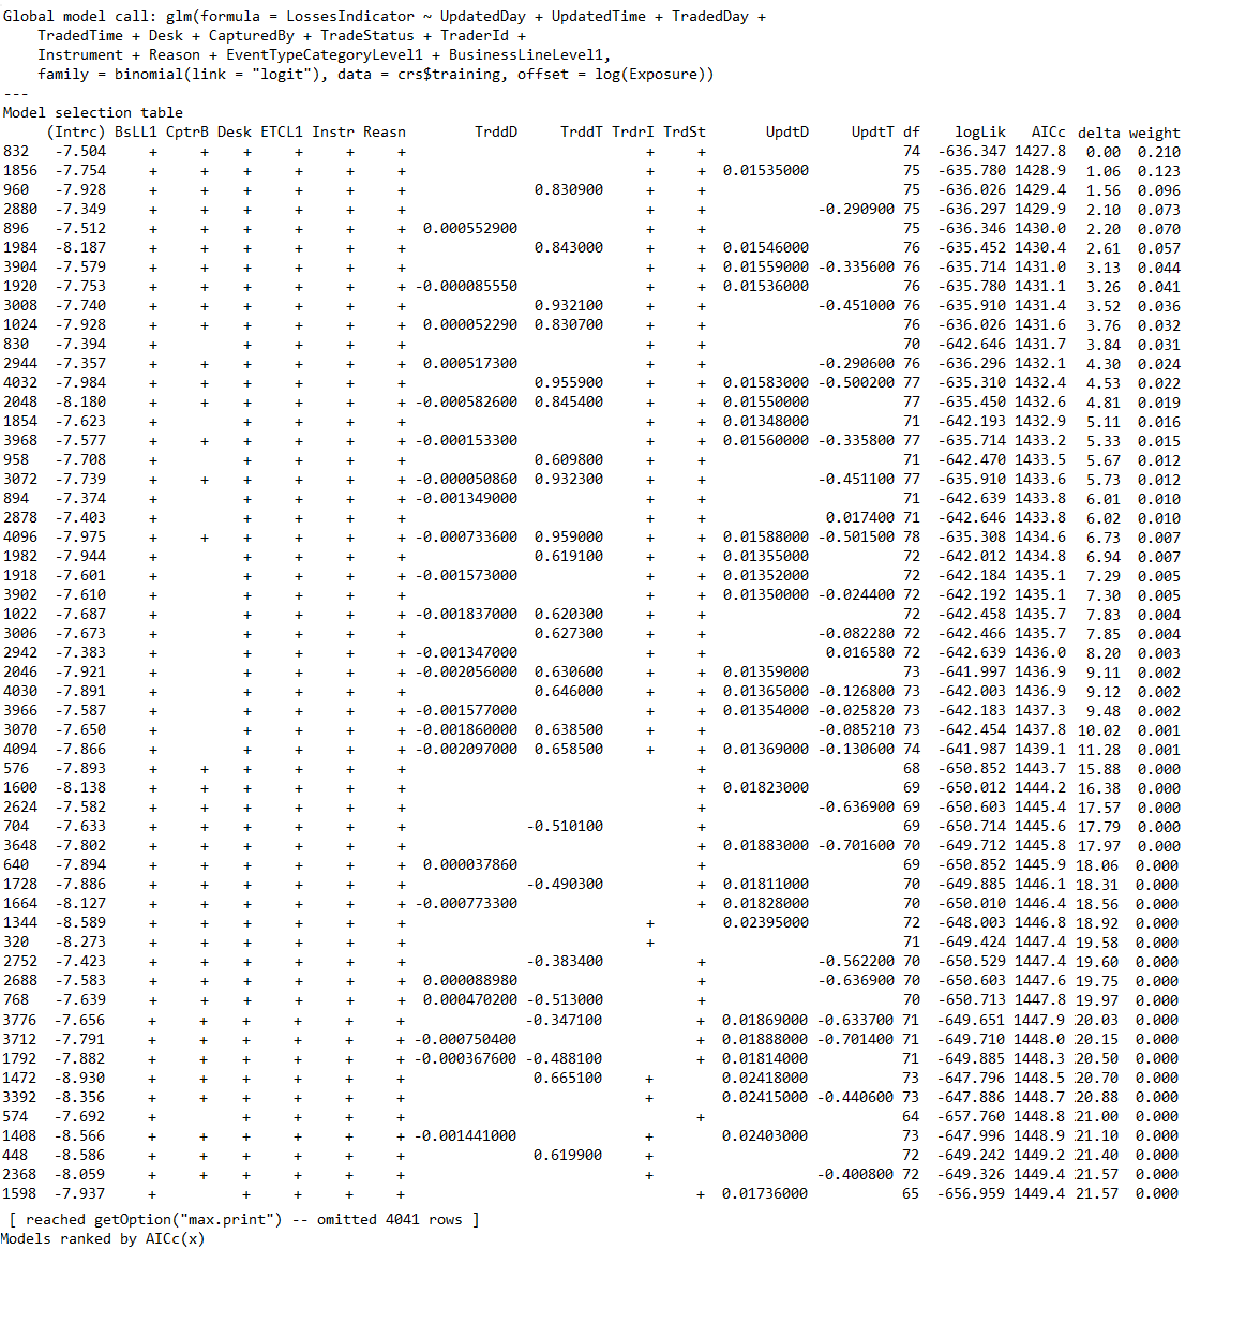
\includegraphics[height=20cm, width=15cm]{Dredge_bin.pdf}
\caption[Data dredging]{Model selection data mining exercise}
\label{Dredge}
\end{figure}

\subsection{We use \texttt{get.models} function to generate a list in which its objects are the fitted models. We will also use the "model.avg" function to do a model averaging based on AICc.}
\label{sec:Model averaging function}

\small

\begin{verbatim}
cl <- makeCluster(2) # Assign R cores to the job 
Amodel <- model.avg(get.models(freqfits, subset = TRUE))
summary(Amodel)
stopCluster(cl) 
\end{verbatim}

\normalsize

Now we have AICc values for our models and we have the average model (or
mean model).

\begin{figure}
\centering
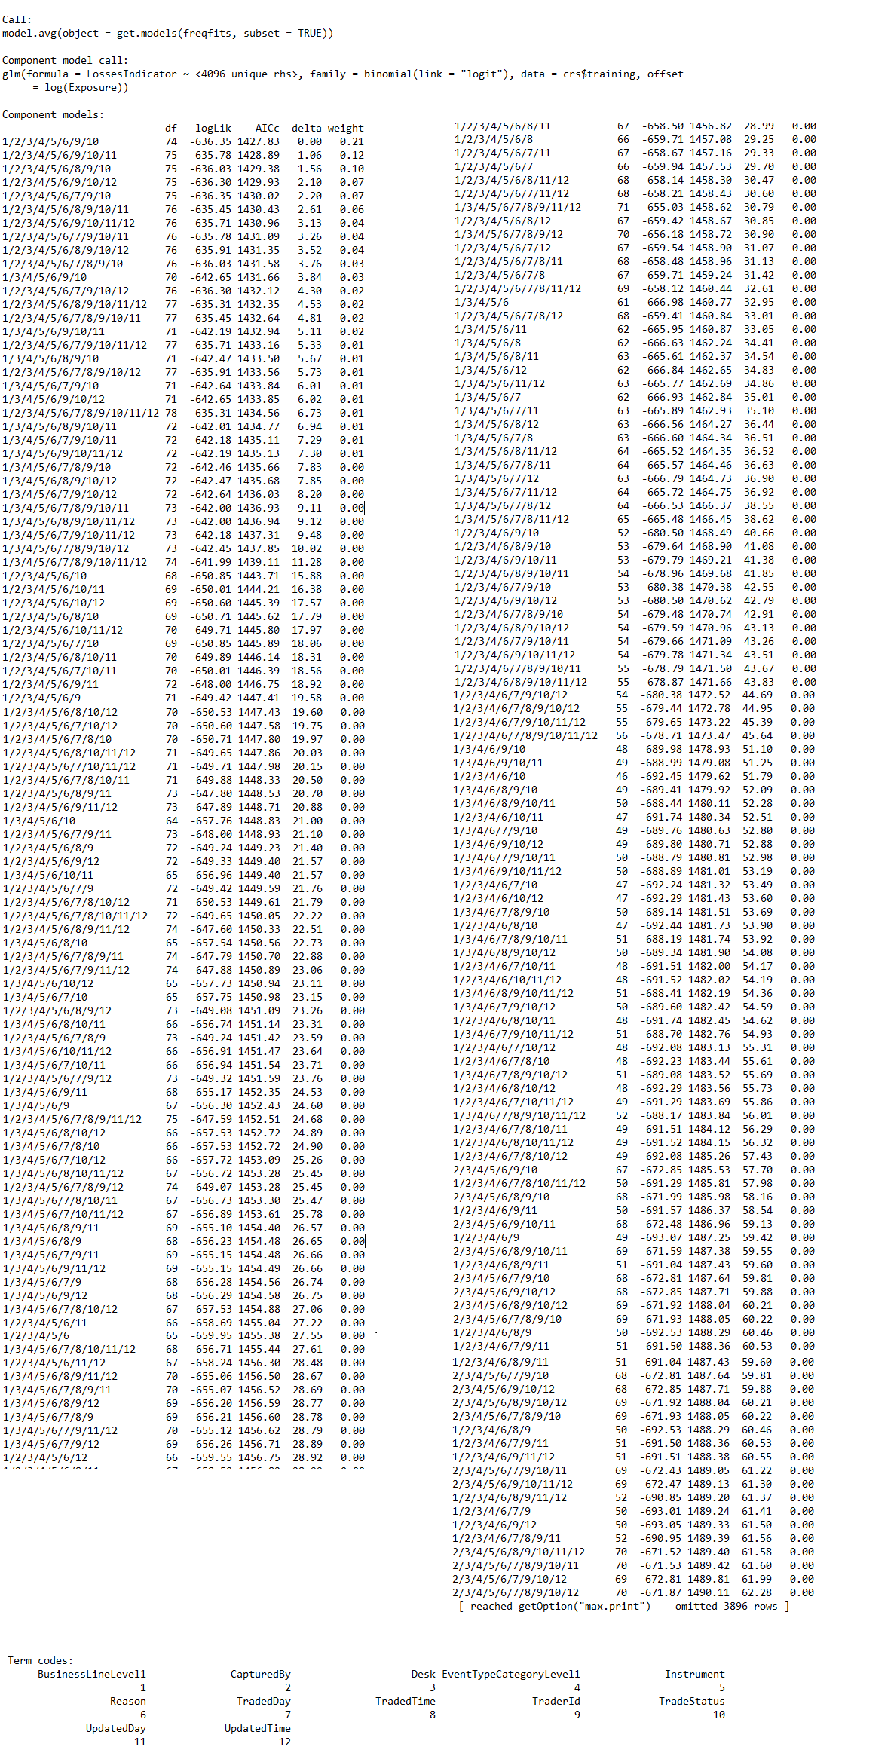
\includegraphics[height=20cm, width=15cm]{Get_models_bin1.pdf}
\caption[Model averaging components]{Estimation of some Poisson distribution for target variable \texttt{LossesIndicator} showing the 4096 component models and their respective AICc values for our models giving rise to the average (mean) model \texttt{Amodel}}
\label{AModel_Summary1}
\end{figure}

\begin{figure}
\centering
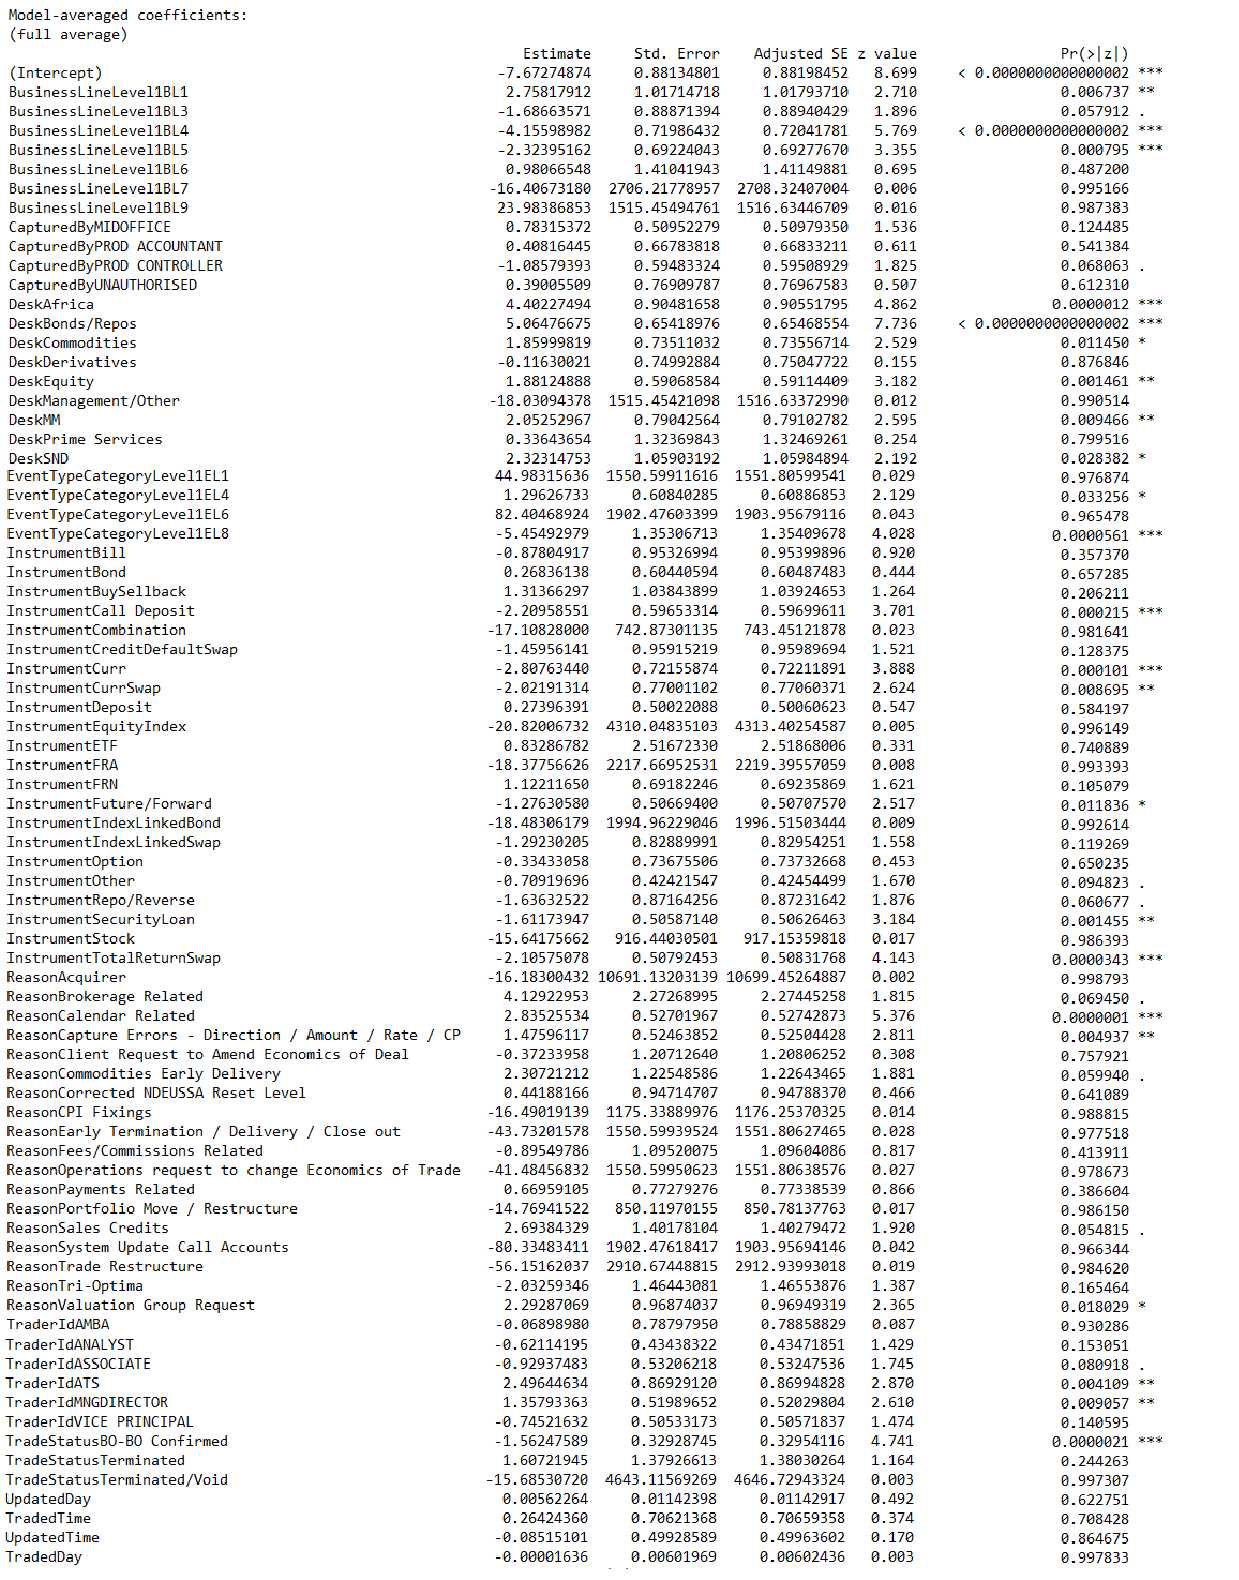
\includegraphics[height=20cm, width=15cm]{Get_models_bin2.pdf}
\caption[Poisson GLM Amodel summary statistics]{Continued from \ref{AModel_Summary1}}
\label{AModel_Summary2}
\end{figure}

\begin{figure}
\centering
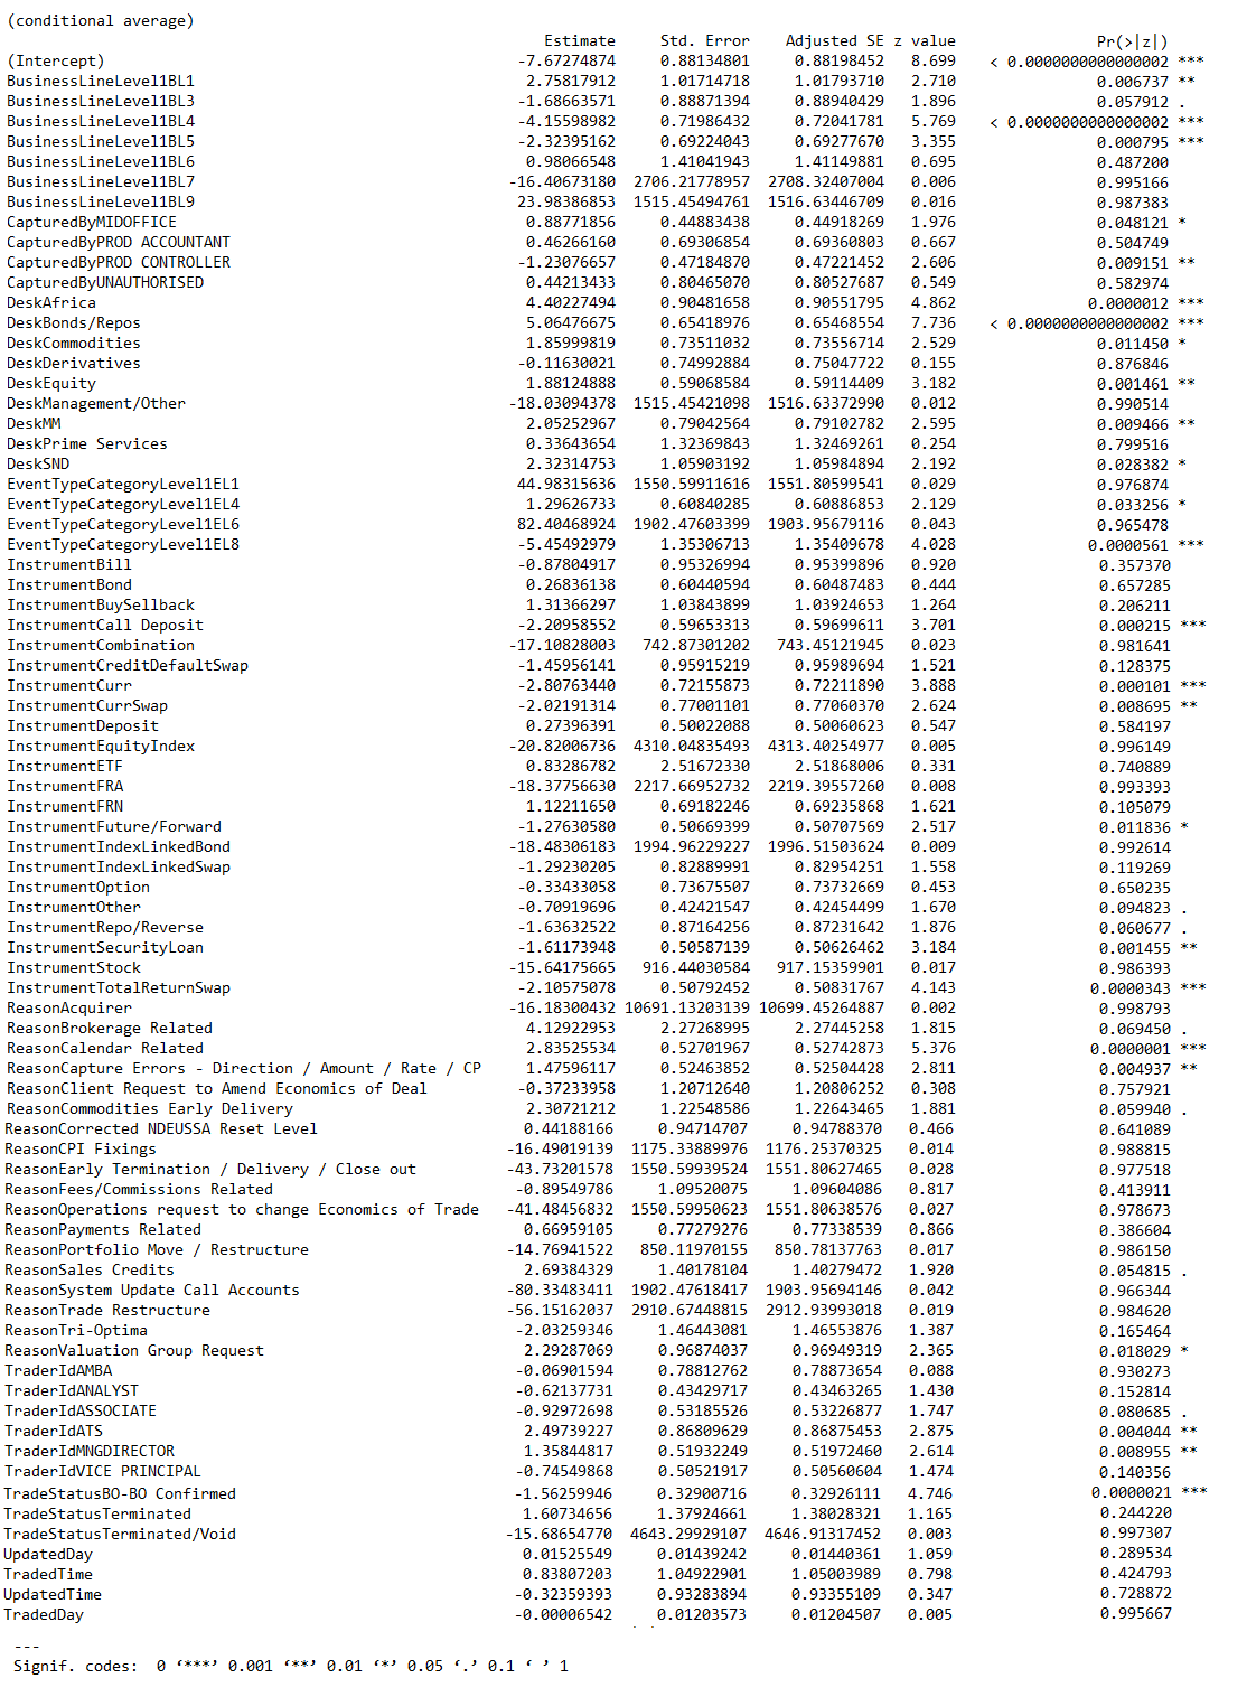
\includegraphics[height=20cm, width=15cm]{Get_models_bin3.pdf}
\caption[Poisson GLM Amodel summary statistics continued]{Continued from \ref{AModel_Summary2}}
\label{Poisson GLM Amodel summary statistics continued}
\end{figure}

\subsection{Evaluate model performance on the test dataset}
\label{sec:Evaluate model performance on the test dataset}

Obtain the response from the Linear model.

\small

\begin{verbatim}
 Av.PredTT <- predict(Amodel, crs$testing, type = "response")
 
 # Export into excel
 
HTMLStart(); HTML(data.frame(Av.PredTT)); w <- HTMLStop()
browseURL(w)
 
shell(paste("start excel", w))
Est <- "file:///C:/Users/Mphekeleli/Documents/R PROJECT/OpRiskPHDGitHub/
OpRisk_PHD_Thesis/Data/OPriskDataSet_GoF_Amodel_InCode.csv"
pred <- read.csv(Est,
                   sep=",",
                   dec=".",
                   na.strings=c(".", "NA", "", "?"),
                   strip.white=TRUE, encoding="UTF-8")
\end{verbatim}

\normalsize

Generate the confusion matrix showing counts and generate an ROC curve
for the GLM model on the appropriate dataset partition

\begin{verbatim}
confusionMatrix(table(pred$response, crs[["testing"]][["LossesIndicator"]]))

crs$pr <- Av.PredTT

# Remove observations with missing target.

no.miss   <- na.omit(crs[["testing"]][["LossesIndicator"]])
miss.list <- attr(no.miss, "na.action")
attributes(no.miss) <- NULL

if (length(miss.list))
{
  predic <- prediction(crs$pr[-miss.list], no.miss)
} else
{
  predic <- prediction(crs$pr, no.miss)
}

pe <- performance(predic, "tpr", "fpr")
au <- performance(predic, "auc")@y.values[[1]]
pd <- data.frame(fpr=unlist(pe@x.values), tpr=unlist(pe@y.values))
p <- ggplot(pd, aes(x=fpr, y=tpr))
p <- p + geom_line(colour="red")
p <- p + xlab("False Positive Rate") + ylab("True Positive Rate")
p <- p + ggtitle("ROC Curve Linear OPriskDataSet_exposure.csv [validate] LossesIndicator")
p <- p + theme(plot.title=element_text(size=10))
p <- p + geom_line(data=data.frame(), aes(x=c(0,1), y=c(0,1)), colour="grey")
p <- p + annotate("text", x=0.50, y=0.00, hjust=0, vjust=0, size=5,
                  label=paste("AUC =", round(au, 2)))
print(p)

# Calculate the area under the curve for the plot.


# Remove observations with missing target.

no.miss   <- na.omit(crs[["testing"]][["LossesIndicator"]])
miss.list <- attr(no.miss, "na.action")
attributes(no.miss) <- NULL

if (length(miss.list))
{
  predic <- prediction(crs$pr[-miss.list], no.miss)
} else
{
  predic <- prediction(crs$pr, no.miss)
}
performance(predic, "auc")
\end{verbatim}

\begin{figure}
\centering
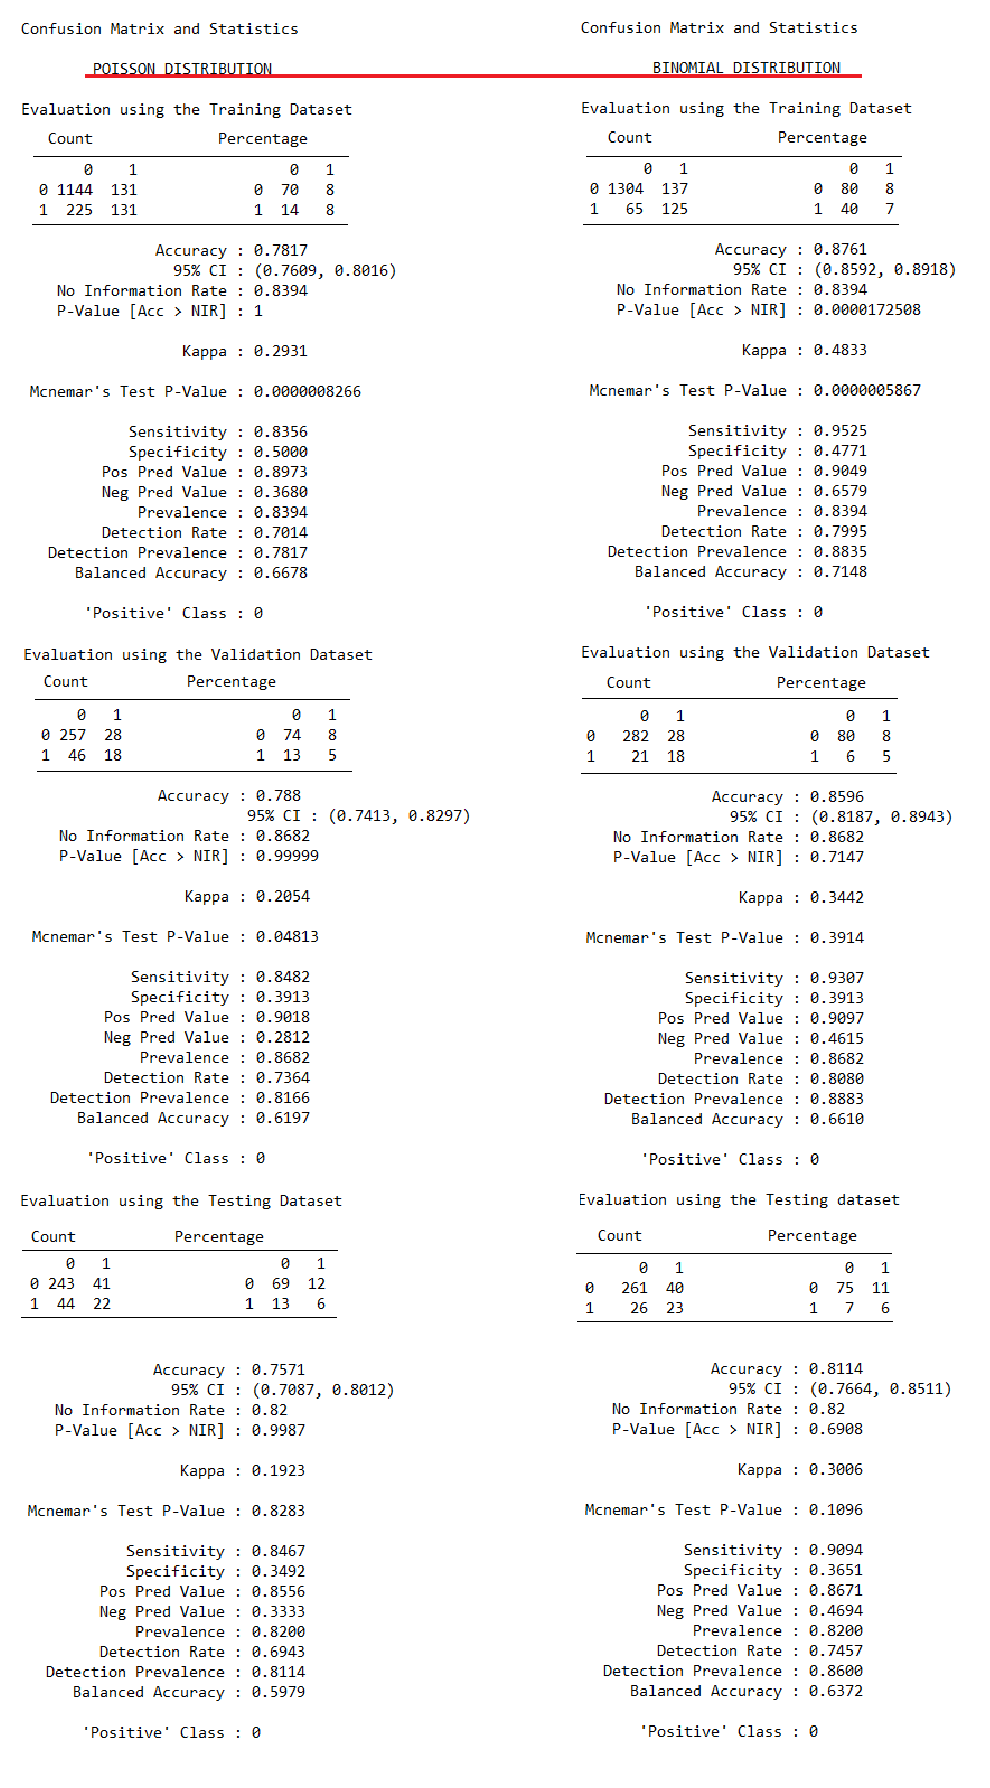
\includegraphics[height=20cm, width=15cm]{ConfusionMatrix_Appendix.eps}
\caption[Confusion Matrices comparison]{Comparison of Poisson, Binomial GLM's confusion matrices for Training, Validation \& Testing datasets}
\label{ConfusionMatrixAll}
\end{figure}

\begin{figure}[t!] % "[t!]" placement specifier just for this example
\begin{subfigure}{0.48\textwidth}
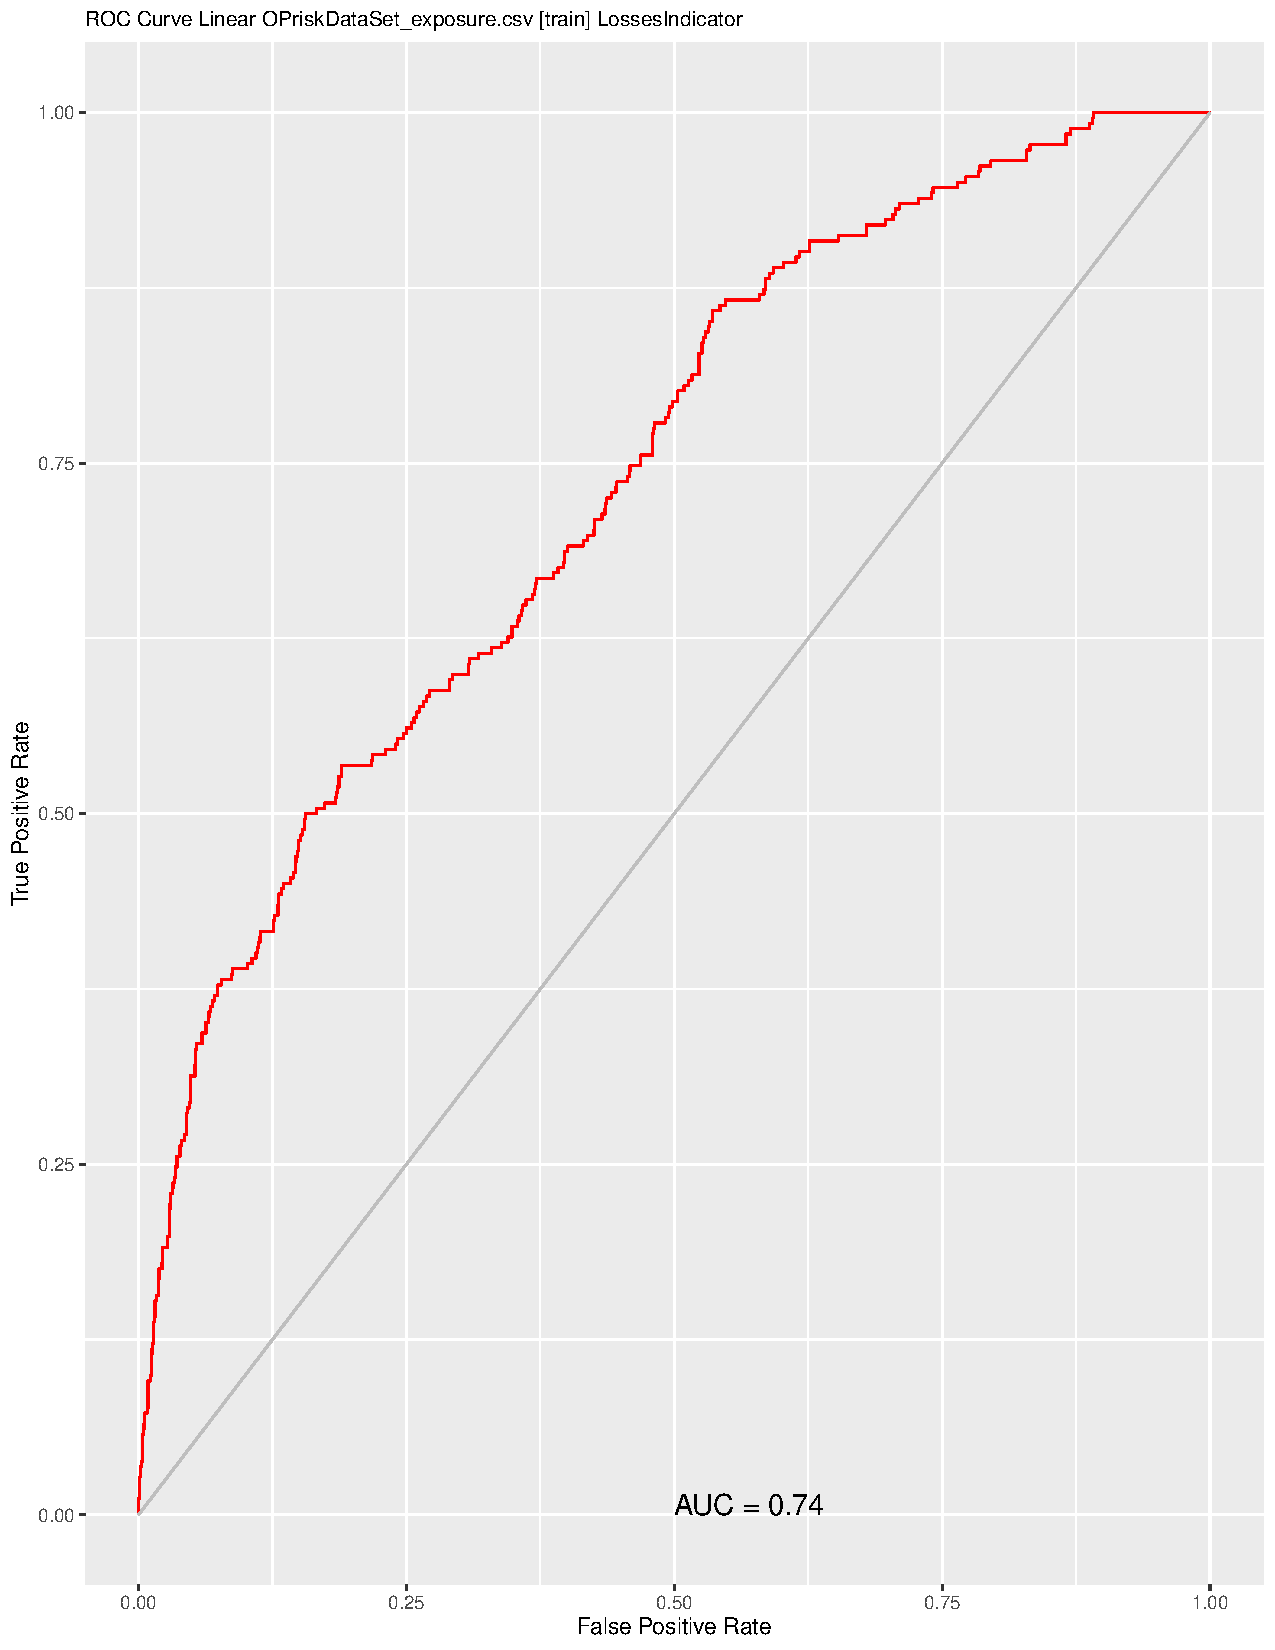
\includegraphics[width=\linewidth, height=5cm]{POI_ROC_Training.pdf}
\caption{AUC for poisson parameter depicting model's performance on the training set} \label{POI_ROC_Train}
\end{subfigure}\hspace*{\fill}
\begin{subfigure}{0.48\textwidth}
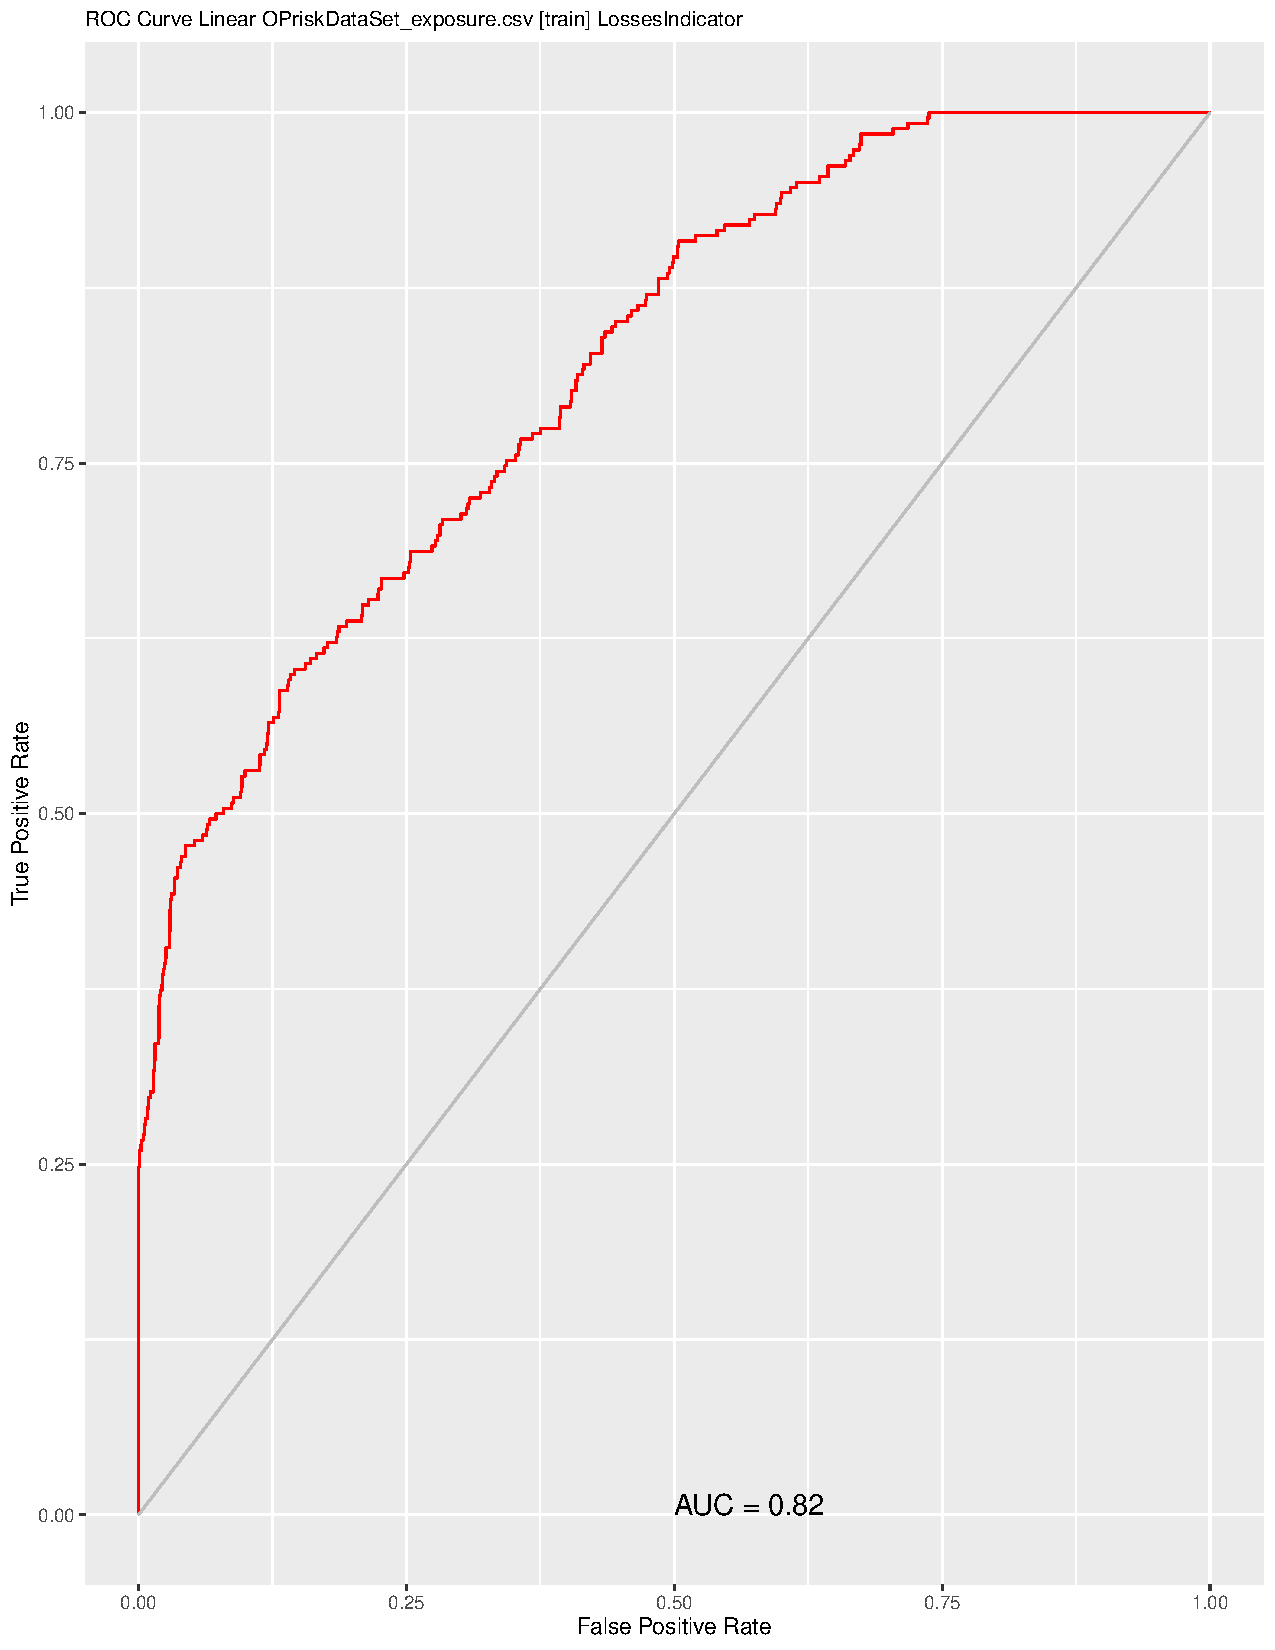
\includegraphics[width=\linewidth, height=5cm]{BIN_ROC_Training.pdf}
\caption{AUC for binomial parameters depicting model's performance on the training set} \label{BIN_ROC_Train}
\end{subfigure}

\medskip
\begin{subfigure}{0.48\textwidth}
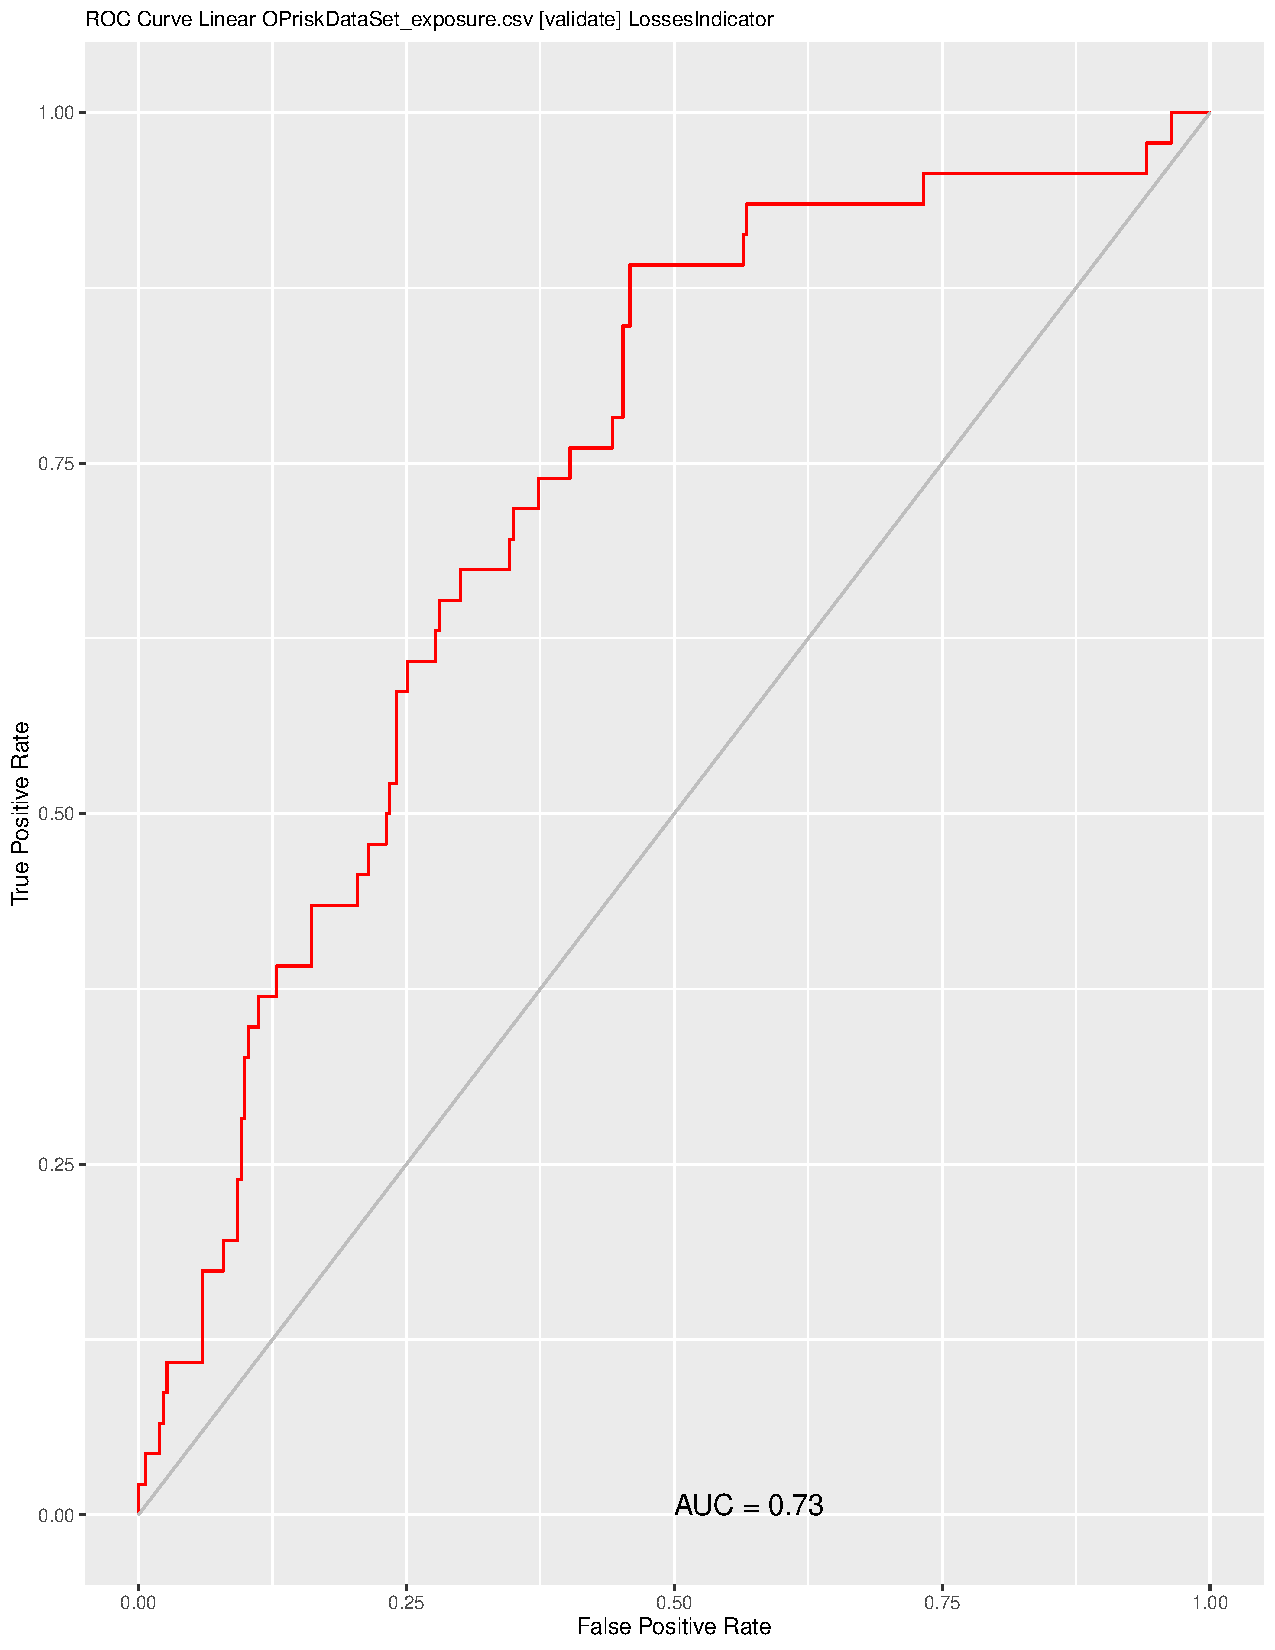
\includegraphics[width=\linewidth, height=5cm]{POI_ROC_Validation.pdf}
\caption{As in (a) but depicting model's performance on the validation set} \label{POI_ROC_Validate}
\end{subfigure}\hspace*{\fill}
\begin{subfigure}{0.48\textwidth}
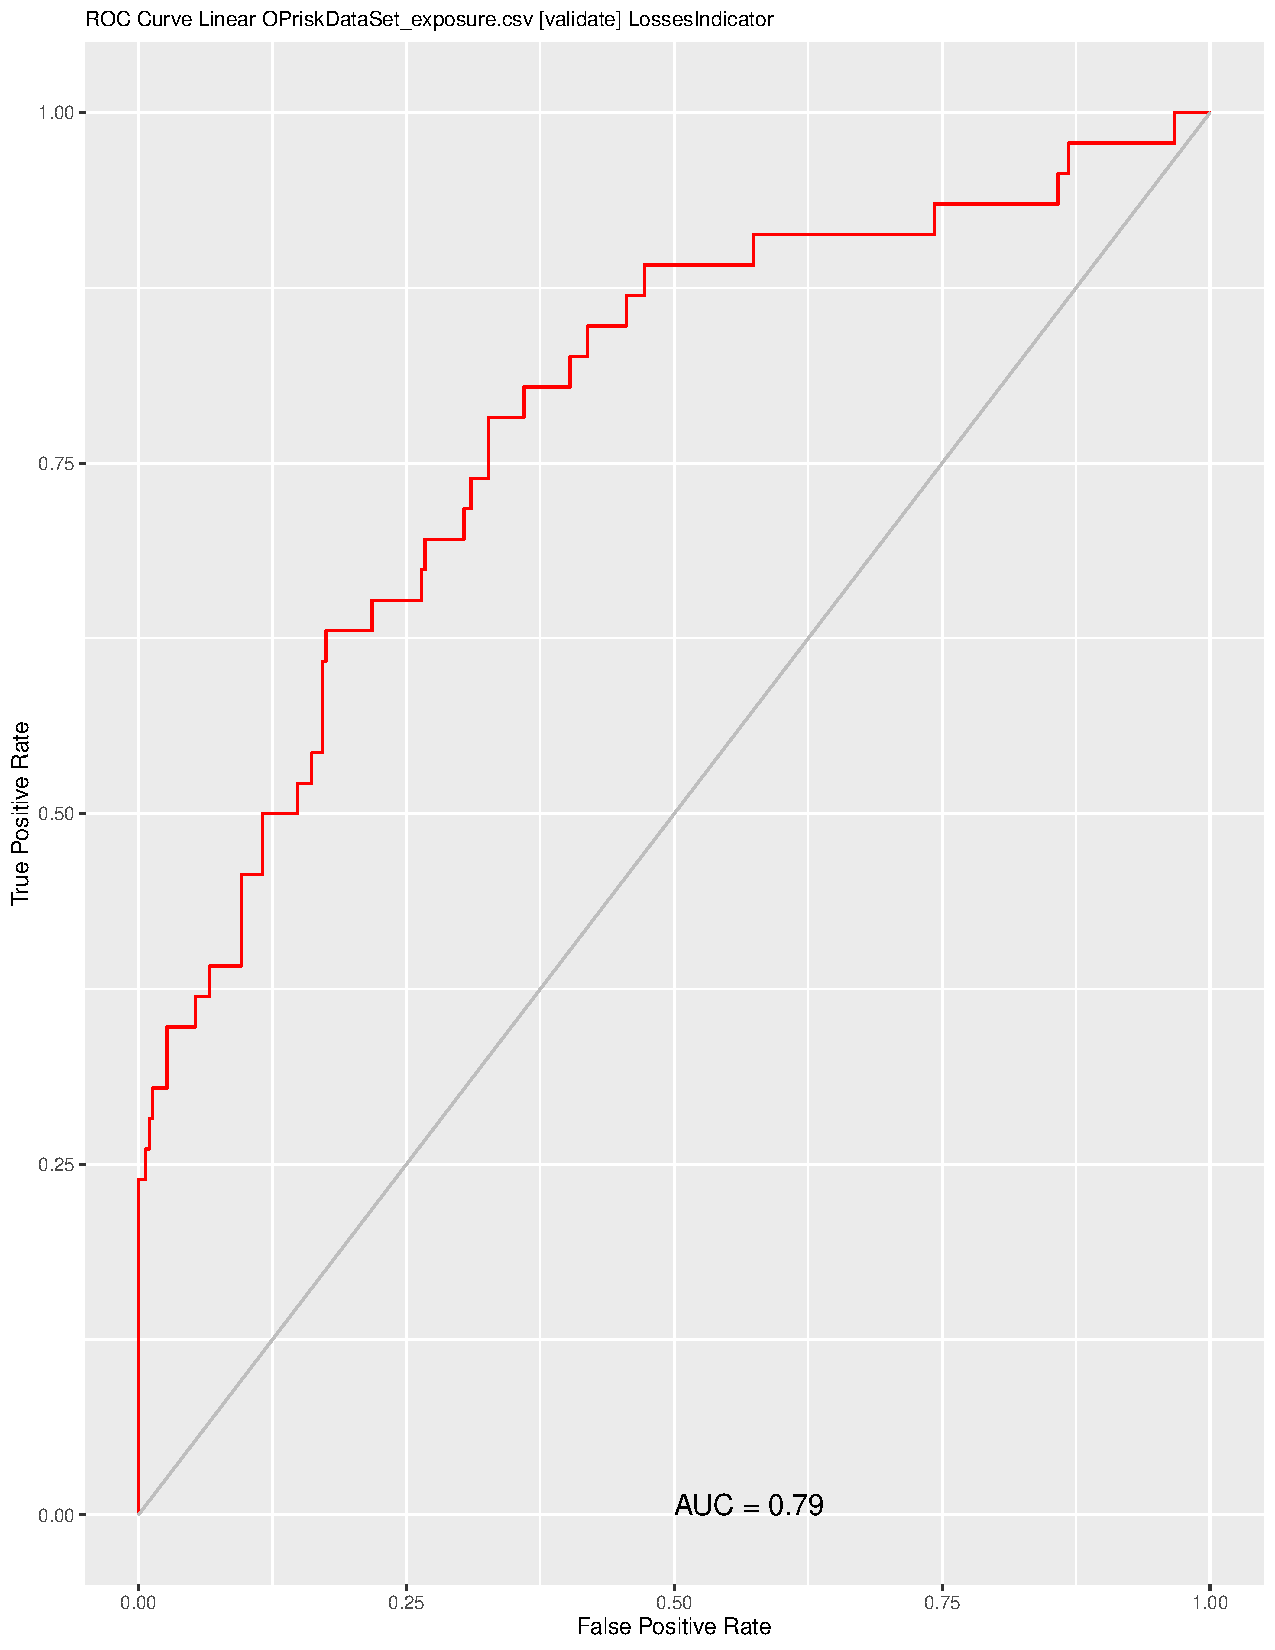
\includegraphics[width=\linewidth, height=5cm]{BIN_ROC_Validation.pdf}
\caption{As in (b) but depicting model's performance on the validation set} \label{BIN_ROC_Validate}
\end{subfigure}

\medskip
\begin{subfigure}{0.48\textwidth}
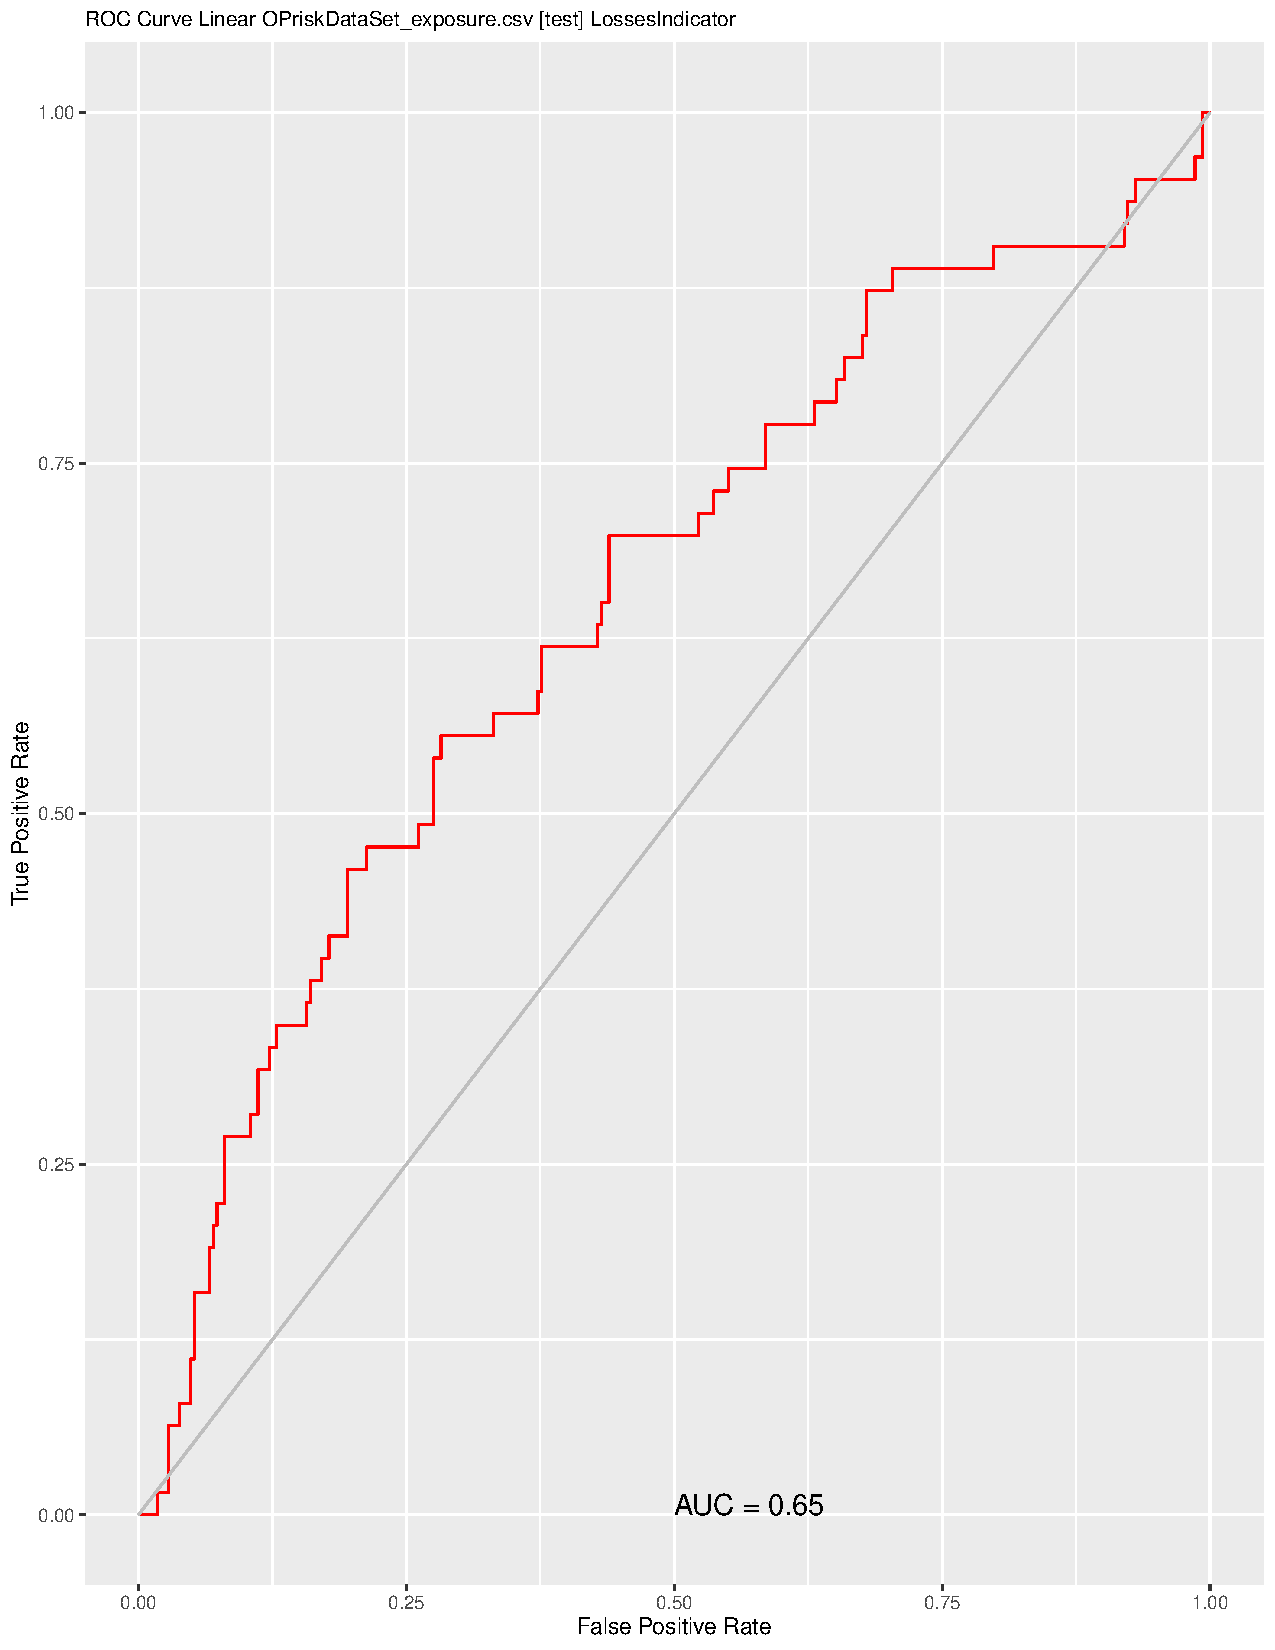
\includegraphics[width=\linewidth, height=5cm]{POI_ROC_Testing.pdf}
\caption{As in (a) \& (c) depicting model's performance on the testing set} \label{POI_ROC_Test}
\end{subfigure}\hspace*{\fill}
\begin{subfigure}{0.48\textwidth}
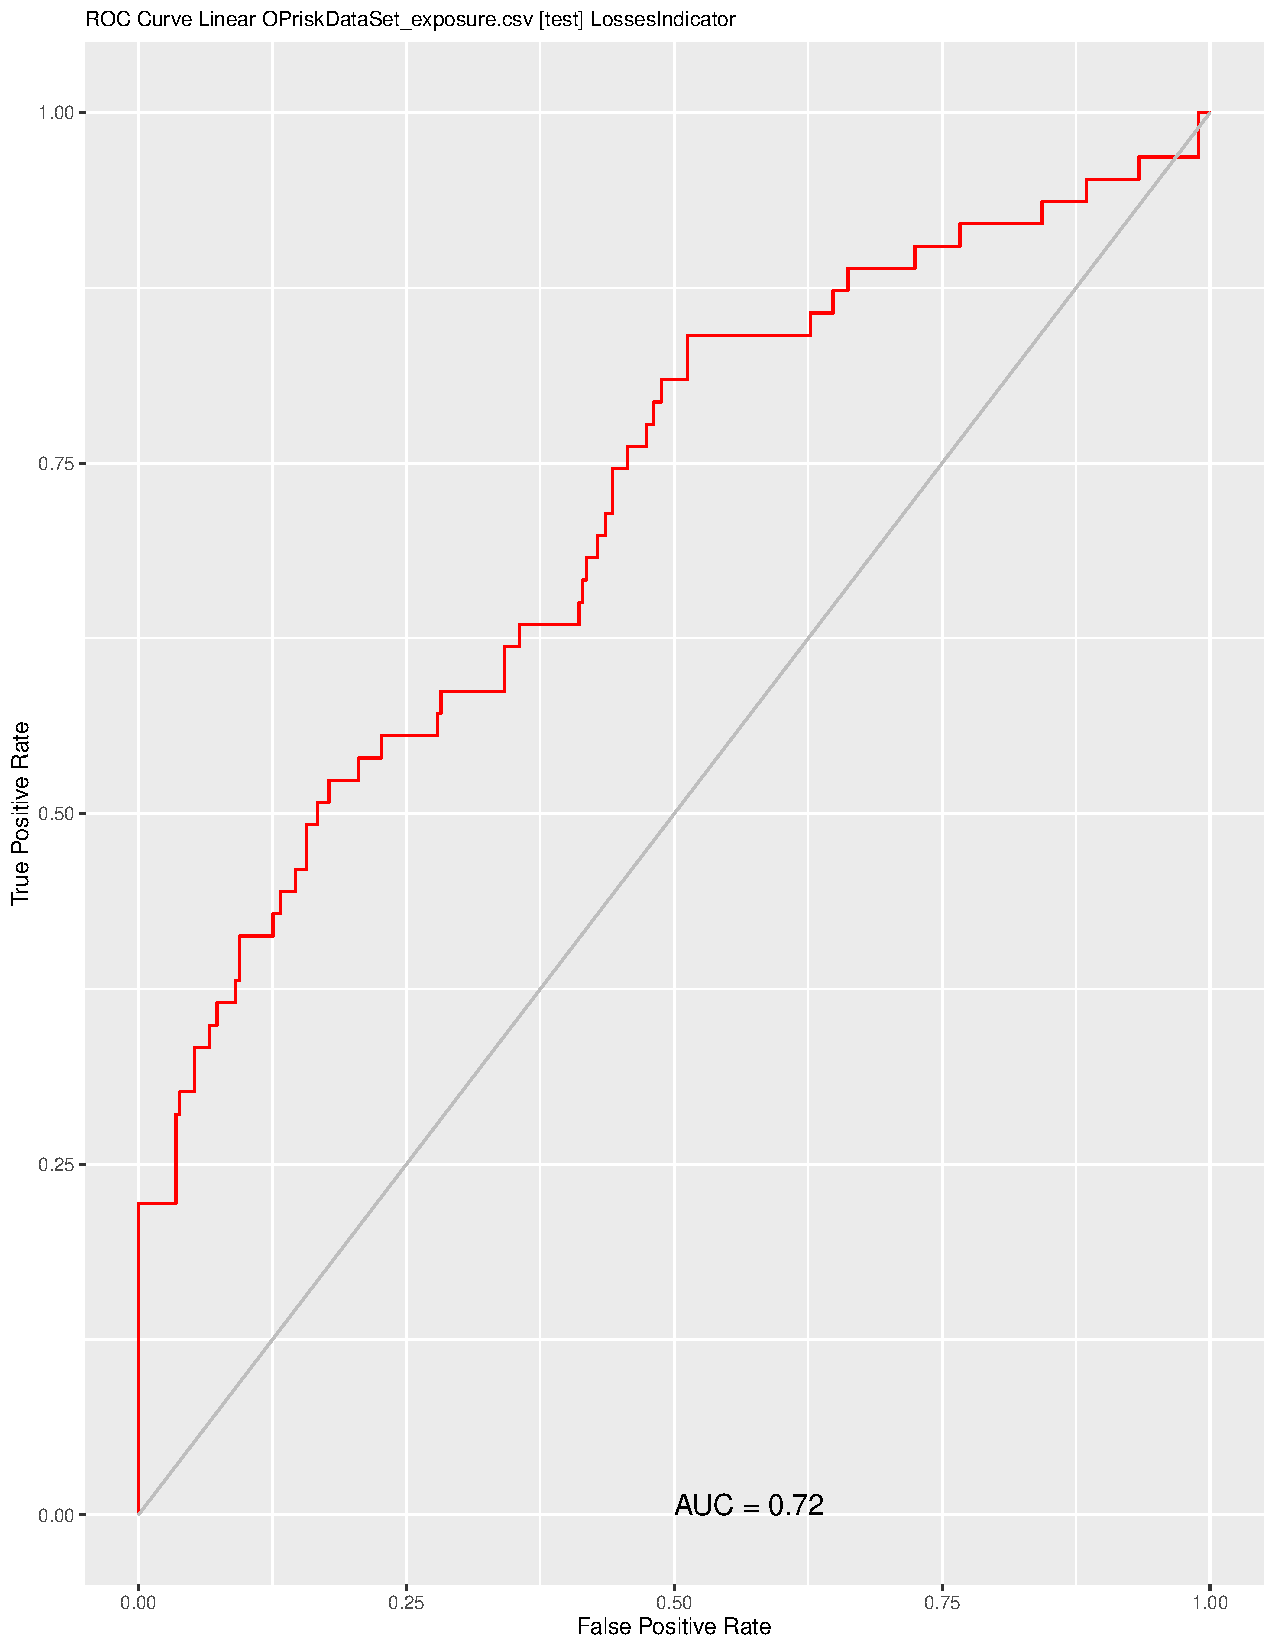
\includegraphics[width=\linewidth, height=5cm]{BIN_ROC_Testing.pdf}
\caption{As in (b) \& (d) depicting model's performance on the testing set} \label{BIN_ROC_Test}
\end{subfigure}

\caption{Comparison of area under the curve (AUC) for the Poisson, Binomial GLM ROC curve for training, validation and testing datasets} \label{ROCCurveAll}
\end{figure}

\clearpage

\section{Data augmentation code: Extrapolation simulation in Matlab}
\label{sec:Data augmentation code: Extrapolation simulation in Matlab}

Notably, the code for the predict condition was run via the Matlab
Terminal:

\small

\begin{verbatim}

% Updated Time
% generate the vector DD

DDD = 1:31;

% generate the vector VVV

VVV = 1:12;

% generate the vector UUU

UUU = 2013 : -1 : 2006;

% making the full thrity five days vector
% Years
Thirty_five_days = [UUU';UUU';UUU';UUU(1:end-1)'];
%Months
Thirty_five_days2 = [VVV';VVV';VVV(1:7)'];
% Days
Thirty_five_days3 = DDD';

% The updated time algorithm

% initializing the time matrix
for i = 1 : length(UUU)
    
    UUU_trans{i} = num2cell(zeros(1,12));
    
end

for i = 1 : length(UUU)
    for j = 1 : length(UUU_trans{1,1})
        
        UUU_TRANS{1,i}{1,j} = num2cell(zeros(31,4));
    end
    
end

% The number of random numbers
H = 1000;
UPD =.789155092592539;
format long
% filling in the time matrix
for i = 1 : length(UUU)
    for j = 1 : length(UUU_trans{1,1})
        
        UUU_TRANS{1,i}{1,j}(:,end) = num2cell((1:31)');
        UUU_TRANS{1,i}{1,j}(:,end-1) = num2cell(VVV(j));
        
        
        
    end
    
end

UUU = num2cell(UUU);
%         UUU = sortrows(UUU,2);


for i = 1 : length(UUU)
    for j = 1 : length(UUU_trans{1,1})
        for k = 1 : length(UUU_TRANS{1,5}{1,1})
            % PART 1
            UUU{i,j} =num2cell((((i)^(0)).*((j)^(0)).*rand(1,31)));
            UUU{i,j} = UUU{i,j}';
            UUU{i,j}(:,2) = num2cell(Thirty_five_days(:,1));
            UUU{i,j} = sortrows(UUU{i,j},1);
            
            %PART 2
            UUU2{i,j} =num2cell((((i)^(0)).*((j)^(0)).*rand(1,31)));
            UUU2{i,j} = UUU2{i,j}';
            UUU2{i,j}(:,2) = num2cell(Thirty_five_days2(:,1));
            UUU2{i,j} = sortrows(UUU2{i,j},1);
            % PART 3
            UUU3{i,j} =num2cell((((i)^(0)).*((j)^(0)).*rand(1,31)));
            UUU3{i,j} = UUU3{i,j}';
            UUU3{i,j}(:,2) = num2cell(Thirty_five_days3(:,1));
            UUU3{i,j} = sortrows(UUU3{i,j},1);
            % PART 1
            UUU_TRANS{1,i}{1,j}(k,end-3) = UUU{i,j}(k,2);
            
            % PART 2
            UUU_TRANS{1,i}{1,j}(k,end-2) = UUU2{i,j}(k,2);
            %PART3
            UUU_TRANS{1,i}{1,j}(k,end-1) = UUU3{i,j}(k,2);
            rH{i,j} = num2cell(((i)^(0).*(j)^(0)).*rand(H,1));
            yH{i,j} = rH{i,j}(cell2mat( rH{i,j}) <= UPD);
            gH{i,j} = num2cell(cell2mat( yH{i,j}(1:31)));
            UUU_TRANS{1,i}{1,j}(k,end) = gH{i,j}(k,1);
        end
    end
    
end

UPDATED_TIME = UUU_TRANS;


%% Traded time

% generate the vector DD

DDDT = 1:31;

% generate the vector VVV

VVVT = 1:12;

% generate the vector UUU

UUUT = 2013 : -1 : 2006;

% making the full thrity five days vector
% Years
Thirty_five_daysT = [UUUT';UUUT';UUUT';UUUT(1:end-1)'];
%Months
Thirty_five_days2T = [VVVT';VVVT';VVVT(1:7)'];
% Days
Thirty_five_days3T = DDDT';

% The updated time algorithm

% initializing the time matrix
for i = 1 : length(UUUT)
    
    UUU_transT{i} = num2cell(zeros(1,12));
    
end

for i = 1 : length(UUUT)
    for j = 1 : length(UUU_transT{1,1})
        
        UUU_TRANST{1,i}{1,j} = num2cell(zeros(31,4));
    end
    
end

% The number of random numbers
HT = 1000;
UPDT =.789155092592539;
format long
% filling in the time matrix
for i = 1 : length(UUUT)
    for j = 1 : length(UUU_transT{1,1})
        
        UUU_TRANST{1,i}{1,j}(:,end) = num2cell((1:31)');
        UUU_TRANST{1,i}{1,j}(:,end-1) = num2cell(VVVT(j));
        
        
        
    end
    
end

UUUT = num2cell(UUUT);
%         UUU = sortrows(UUU,2);


for i = 1 : length(UUUT)
    for j = 1 : length(UUU_transT{1,1})
        for k = 1 : length(UUU_TRANST{1,5}{1,1})
            % PART 1
            UUUT{i,j} =num2cell((((i)^(0)).*((j)^(0)).*rand(1,31)));
            UUUT{i,j} = UUUT{i,j}';
            UUUT{i,j}(:,2) = num2cell(Thirty_five_daysT(:,1));
            UUUT{i,j} = sortrows(UUUT{i,j},1);
            
            %PART 2
            UUU2T{i,j} =num2cell((((i)^(0)).*((j)^(0)).*rand(1,31)));
            UUU2T{i,j} = UUU2T{i,j}';
            UUU2T{i,j}(:,2) = num2cell(Thirty_five_days2T(:,1));
            UUU2T{i,j} = sortrows(UUU2T{i,j},1);
            % PART 3
            UUU3T{i,j} =num2cell((((i)^(0)).*((j)^(0)).*rand(1,31)));
            UUU3T{i,j} = UUU3T{i,j}';
            UUU3T{i,j}(:,2) = num2cell(Thirty_five_days3T(:,1));
            UUU3T{i,j} = sortrows(UUU3T{i,j},1);
            % PART 1
            UUU_TRANST{1,i}{1,j}(k,end-3) = UUUT{i,j}(k,2);
            
            % PART 2
            UUU_TRANST{1,i}{1,j}(k,end-2) = UUU2T{i,j}(k,2);
            %PART3
            UUU_TRANST{1,i}{1,j}(k,end-1) = UUU3T{i,j}(k,2);
            rHT{i,j} = num2cell(((i)^(0).*(j)^(0)).*rand(HT,1));
            yHT{i,j} = rHT{i,j}(cell2mat( rHT{i,j}) <= UPDT);
            gHT{i,j} = num2cell(cell2mat( yHT{i,j}(1:31)));
            UUU_TRANST{1,i}{1,j}(k,end) = gHT{i,j}(k,1);
        end
    end
    
end

TRADED_TIME = UUU_TRANST;

%% RULE for correcting the traded time
SIZZZE = size(UUU_TRANS{1,3}{1,2});
for i = 1 : 8
    for j = 1 : length(UUU_transT{1,1})
        for k = 1 : length(UUU_TRANST{1,5}{1,1})
            
            
            if  TRADED_TIME{1,i}{1,j}{k,1} >= UPDATED_TIME{1,i}{1,j}{k,1}
                
                TRADED_TIME{1,i}{1,j}{k,1} = UPDATED_TIME{1,i}{1,j}{k,1};
            end
                
            if TRADED_TIME{1,i}{1,j}{k,1} >= UPDATED_TIME{1,i}{1,j}{k,1}...
                    && TRADED_TIME{1,i}{1,j}{k,2} >= UPDATED_TIME{1,i}{1,j}{k,2}
                
                
                TRADED_TIME{1,i}{1,j}{k,1} = UPDATED_TIME{1,i}{1,j}{k,1};
                TRADED_TIME{1,i}{1,j}{k,2} = UPDATED_TIME{1,i}{1,j}{k,2};
            end
                
                
                
            if TRADED_TIME{1,i}{1,j}{k,1} >= UPDATED_TIME{1,i}{1,j}{k,1}...
                    && TRADED_TIME{1,i}{1,j}{k,2} >= UPDATED_TIME{1,i}{1,j}{k,2}...
                    && TRADED_TIME{1,i}{1,j}{k,3} >= UPDATED_TIME{1,i}{1,j}{k,3}
                
                
                TRADED_TIME{1,i}{1,j}{k,1} = UPDATED_TIME{1,i}{1,j}{k,1};
                TRADED_TIME{1,i}{1,j}{k,2} = UPDATED_TIME{1,i}{1,j}{k,2};
                TRADED_TIME{1,i}{1,j}{k,3} = UPDATED_TIME{1,i}{1,j}{k,3};
            end
                
                
            if TRADED_TIME{1,i}{1,j}{k,1} >= UPDATED_TIME{1,i}{1,j}{k,1}...
                    && TRADED_TIME{1,i}{1,j}{k,2} >= UPDATED_TIME{1,i}{1,j}{k,2}...
                    && TRADED_TIME{1,i}{1,j}{k,3} >= UPDATED_TIME{1,i}{1,j}{k,3}...
                    && TRADED_TIME{1,i}{1,j}{k,4} >= UPDATED_TIME{1,i}{1,j}{k,4}
                
                
                
                TRADED_TIME{1,i}{1,j}{k,1} = UPDATED_TIME{1,i}{1,j}{k,1};
                TRADED_TIME{1,i}{1,j}{k,2} = UPDATED_TIME{1,i}{1,j}{k,2};
                TRADED_TIME{1,i}{1,j}{k,3} = UPDATED_TIME{1,i}{1,j}{k,3};
                TRADED_TIME{1,i}{1,j}{k,4} = UPDATED_TIME{1,i}{1,j}{k,4};
                
            end
        end
    end
    
end

%% The traded time table
% Fill the updated time
for i = 1 : 8
    
   TABLE_TRADED_TIME{1,i} = vertcat(TRADED_TIME{1,i}{1,1},...
       TRADED_TIME{1,i}{1,2}, TRADED_TIME{1,i}{1,3},...
       TRADED_TIME{1,i}{1,4}, TRADED_TIME{1,i}{1,5},...
       TRADED_TIME{1,i}{1,6}, TRADED_TIME{1,i}{1,7},...
       TRADED_TIME{1,i}{1,8}, TRADED_TIME{1,i}{1,9},...
       TRADED_TIME{1,i}{1,10}, TRADED_TIME{1,i}{1,11},...
       TRADED_TIME{1,i}{1,12});
    
end

% The final concatenation
FINAL_TABLE_TRADED_TIME = vertcat(TABLE_TRADED_TIME{1,1},...
    TABLE_TRADED_TIME{1,2},TABLE_TRADED_TIME{1,3},...
    TABLE_TRADED_TIME{1,4},TABLE_TRADED_TIME{1,5},...
    TABLE_TRADED_TIME{1,6},TABLE_TRADED_TIME{1,7},...
    TABLE_TRADED_TIME{1,8});


%% The updated time table
% Fill the updated time
for i = 1 : 8
    
   TABLE_UPDATED_TIME{1,i} = vertcat(UPDATED_TIME{1,i}{1,1},...
       UPDATED_TIME{1,i}{1,2}, UPDATED_TIME{1,i}{1,3},...
       UPDATED_TIME{1,i}{1,4}, UPDATED_TIME{1,i}{1,5},...
       UPDATED_TIME{1,i}{1,6}, UPDATED_TIME{1,i}{1,7},...
       UPDATED_TIME{1,i}{1,8}, UPDATED_TIME{1,i}{1,9},...
       UPDATED_TIME{1,i}{1,10}, UPDATED_TIME{1,i}{1,11},...
       UPDATED_TIME{1,i}{1,12});
    
end

% The final concatenation
FINAL_TABLE_UPDATED_TIME = vertcat(TABLE_UPDATED_TIME{1,1},...
    TABLE_UPDATED_TIME{1,2},TABLE_UPDATED_TIME{1,3},...
    TABLE_UPDATED_TIME{1,4},TABLE_UPDATED_TIME{1,5},...
    TABLE_UPDATED_TIME{1,6},TABLE_UPDATED_TIME{1,7},...
    TABLE_UPDATED_TIME{1,8});

% Find the unique traded times, Sort the traded times and assign
% unique trade number to each in ascending order
UNIQ = sortrows(unique(cell2mat(FINAL_TABLE_TRADED_TIME),'rows'),[1 2 3 4]);
UNIQO = sortrows(unique(cell2mat(FINAL_TABLE_TRADED_TIME),'rows'),[1 2 3 4]);

% generate a random number
raNDgen1 = (324434 : 26835144)';
raNDgen2 = rand(length(raNDgen1),1);

% merge the two vectors
raNDgen = [raNDgen1, raNDgen2];
% sort according to the second column
Sort_raNDgen = sortrows(raNDgen,2);

% Cut at 2976 and sort according to the first column
Sort_raNDgen1 = Sort_raNDgen(1: length(FINAL_TABLE_TRADED_TIME), :);
Sort_raNDgen2 = sortrows(Sort_raNDgen1,1);

% assign the computed trade numbers to the corresponding trade times
UNIQO(:,5) = Sort_raNDgen2(:,1);
% size of UNIQO
SASS = size(UNIQO);
% finding the position of the sorted traded times in the original times
for i = 1 : length(FINAL_TABLE_TRADED_TIME)
POS{i,1} = num2cell(find(ismember(cell2mat(FINAL_TABLE_TRADED_TIME(:,1:end)),UNIQO(i,1:4),'rows')~=0));
end


%% THE_FINAL_TRADED_TIME
THE_FINAL_TRADED_TIME = zeros(length(FINAL_TABLE_TRADED_TIME), SASS(2));

for i = 1 : length(FINAL_TABLE_TRADED_TIME)
    
THE_FINAL_TRADED_TIME(cell2mat(POS{i,1}),:) = UNIQO(i,:);   
       
end

 Headers = OPriskDataSetexposure(1,:);

MATRIX = zeros(length(FINAL_TABLE_TRADED_TIME),length(Headers));

%% The traded time

% converting time into usal time formats
% there are 24 hours in the a day , to fins the hour
rt = 24.*THE_FINAL_TRADED_TIME(:,end-1);
hh = round(rt);

% the minutes
rr = 60.*abs(rt - hh);

mm = round(rr);

% the seconds
rg = 60.*abs(rr - mm);

ss = round(rg);

% Updated time as a vectors
Vec_tedTime = [THE_FINAL_TRADED_TIME(:,1:end-2), hh, mm, ss];

% converting the date back to string
formatOut = 'yyyy-mm-dd HH:MM:SS PM';
Vec_tradedTimeSTRING = datestr(Vec_tedTime(:, 1:end),formatOut);

%% The updated time
% converting time into usal time formats
% there are 24 hours in the a day , to fins the hour
rt = 24.*cell2mat(FINAL_TABLE_UPDATED_TIME(:,end));
hh = round(rt);

% the minutes
rr = 60.*abs(rt - hh);

mm = round(rr);

% the seconds
rg = 60.*abs(rr - mm);

ss = round(rg);

% Updated time as a vectors
Vec_updatedTime = [cell2mat(FINAL_TABLE_UPDATED_TIME(:,1:end-1)), hh, mm, ss];

% converting the date back to string
formatOut = 'yyyy-mm-dd HH:MM:SS PM';
Vec_updatedTimeSTRING = datestr(Vec_updatedTime(:, 1:end),formatOut);

%% generate the compatible columns
% capturedBy
UNI_STRINGS = unique(OPriskDataSetexposure(2:end,9));
% TraderID
UNI_STRINGS1 = unique(OPriskDataSetexposure(2:end,11));

for j = 1 : length(UNI_STRINGS)
    
    CapturedBy{j} = OPriskDataSetexposure(strcmp(OPriskDataSetexposure(:,9),...
        UNI_STRINGS(j))==1,9);
    % percentage proportion
    LEngC(j) = length(CapturedBy{j})./length(OPriskDataSetexposure);
    format long
   N_STR(j) = ceil(LEngC(j).* length(THE_FINAL_TRADED_TIME));
   
   N_STRRR{j} = num2cell(zeros(N_STR(j),1));
   
end


for j = 1 : length(UNI_STRINGS)
   N_STRRR{j}(:,1) = (UNI_STRINGS(j,1));
end
%
CAPTUREDBY_TOTAL = vertcat(N_STRRR{1,1},N_STRRR{1,2},...
    N_STRRR{1,3},N_STRRR{1,4},N_STRRR{1,5});

CAPTUREDBY_TOTAL = CAPTUREDBY_TOTAL(1:length(THE_FINAL_TRADED_TIME));
CAPTUREDBY_TOTAL = [CAPTUREDBY_TOTAL, num2cell(rand(length(CAPTUREDBY_TOTAL),1))];
CAPTUREDBY_TOTAL = sortrows(CAPTUREDBY_TOTAL,2);
%%


%% generate the compatible columns
% TraderID
Tra_UNI_STRINGS = unique(OPriskDataSetexposure(2:end,11));
% TraderID
Tra_UNI_STRINGS1 = unique(OPriskDataSetexposure(2:end,11));

for j = 1 : length(Tra_UNI_STRINGS)
    
    TraderID{j} = OPriskDataSetexposure(strcmp(OPriskDataSetexposure(:,11),...
        Tra_UNI_STRINGS(j))==1,11);
    % percentage proportion
    LEngC(j) = length(TraderID{j})./length(OPriskDataSetexposure);
    format long
   TRAN_STR(j) = ceil(LEngC(j).* length(THE_FINAL_TRADED_TIME));
   
   TRAN_STRRR{j} = num2cell(zeros(TRAN_STR(j),1));
   
end


for j = 1 : length(Tra_UNI_STRINGS)
   TRAN_STRRR{j}(:,1) = (Tra_UNI_STRINGS(j,1));
end

TRADERID_TOTAL = vertcat(TRAN_STRRR{1,1},TRAN_STRRR{1,2},...
    TRAN_STRRR{1,3},TRAN_STRRR{1,4},TRAN_STRRR{1,5},...
    TRAN_STRRR{1,6},TRAN_STRRR{1,7});

 TRADERID_TOTAL = TRADERID_TOTAL(1:length(THE_FINAL_TRADED_TIME));
TRADERID_TOTAL = [TRADERID_TOTAL, num2cell(rand(length(TRADERID_TOTAL),1))];
TRADERID_TOTAL = sortrows(TRADERID_TOTAL,2);
%% Business lines

BL1 = [cellstr('BL1') cellstr('BL1') ;...
    cellstr('Credit Derivatives') cellstr('Investment Banking')]';

BL2 = [cellstr('BL2') cellstr('BL2') cellstr('BL2') cellstr('BL2')...
    cellstr('BL2') cellstr('BL2') cellstr('BL2') cellstr('BL2')...
    cellstr('BL2') cellstr('BL2') cellstr('BL2') cellstr('BL2')...
    cellstr('BL2');...
    cellstr('Rates') cellstr('MM') cellstr('Equity')...
    cellstr('Commodities') cellstr('Africa')...
    cellstr('Options') cellstr('Bonds/Repos')...
    cellstr('Forex') cellstr('Prime Services')...
    cellstr('Credit Derivatives') cellstr('Management')...
    cellstr('Group Treasury') cellstr('SND')]';

BL3 = [cellstr('BL3') cellstr('BL3') cellstr('BL3') ;...
    cellstr('Africa') cellstr('MM') cellstr('SND')]';

BL4 = [cellstr('BL4') cellstr('BL4') cellstr('BL4')...
     cellstr('BL4') cellstr('BL4') cellstr('BL4');...
    cellstr('ACBB') cellstr('Credit Derivatives') cellstr('Funding')...
     cellstr('MM') cellstr('Portfolio Management') cellstr('SND')]';
 
 BL5 = [cellstr('BL5') cellstr('BL5') ;...
    cellstr('Credit Derivatives') cellstr('MM')]';

BL6 = [cellstr('BL6') cellstr('BL6') ;...
    cellstr('Management') cellstr('Prime Services')]';

BL7 = [cellstr('BL7') cellstr('BL7') ;...
    cellstr('Portfolio Management') cellstr('SND')]';

BL9 = [cellstr('BL9') cellstr('Portfolio Management')];

%% generate the compatible columns
% Business line
BUB_UNI_STRINGS = unique(OPriskDataSetexposure(2:end,22));
%
for j = 1 : length(BUB_UNI_STRINGS)
    
    Bus{j} = OPriskDataSetexposure(strcmp(OPriskDataSetexposure(:,22),...
        BUB_UNI_STRINGS(j))==1,22);
    % percentage proportion
    LEngB(j) = length(Bus{j})./length(OPriskDataSetexposure);
    format long
    Bu_STR(j) = ceil(LEngB(j).* length(THE_FINAL_TRADED_TIME));
    
    BUs_STRRR{j} = num2cell(zeros(Bu_STR(j),1));
    
end


for j = 1 : length(BUB_UNI_STRINGS)
    BUs_STRRR{j}(:,1) = (BUB_UNI_STRINGS(j,1));
end
%
BUS_TOTAL = vertcat(BUs_STRRR{1,1},BUs_STRRR{1,2},...
    BUs_STRRR{1,3},BUs_STRRR{1,4},BUs_STRRR{1,5},...
    BUs_STRRR{1,6}, BUs_STRRR{1,7}, BUs_STRRR{1,8});

BUS_TOTAL = BUS_TOTAL(1:length(THE_FINAL_TRADED_TIME));
BUS_TOTAL = [BUS_TOTAL, num2cell(rand(length(BUS_TOTAL),1))];
BUS_TOTAL = sortrows(BUS_TOTAL,2);

%% BUSINESS LINES

BUSINESS_LINESL = [BL1;BL2;BL3;BL4;BL5;BL6;BL7;BL9];

for j = 1 : length(THE_FINAL_TRADED_TIME)
    
    BUSINESS_LINES{j} = num2cell((j.^0).*zeros(length(BUSINESS_LINESL),3));
    BUSINESS_LINES{j}(:,3) = num2cell((j.^0).*rand(length(BUSINESS_LINESL),1));
    BUSINESS_LINES{j}(:,1:2) = BUSINESS_LINESL(:,1:2);
    
    POSITION{j} = find(strcmp(BUSINESS_LINES{j}(:,1),...
        BUS_TOTAL(j,1))==1, 1, 'last' );
    % the desk
    DESK(j,1) = BUSINESS_LINESL(POSITION{j},2);
end
%%
% fill in the matrix
MATRIX(:,1) = (THE_FINAL_TRADED_TIME(:,end));
MATRIX(:,7) = (THE_FINAL_TRADED_TIME(:,end-1));
MATRIX(:,6) = (THE_FINAL_TRADED_TIME(:,end-2));
MATRIX(:,4) = cell2mat(FINAL_TABLE_UPDATED_TIME(:,end));
MATRIX(:,3) = cell2mat(FINAL_TABLE_UPDATED_TIME(:,end-1));


MATRIX = num2cell(MATRIX);

MATRIX(:,8) = DESK(:,1);
MATRIX(:,22) = BUS_TOTAL(:,1);
MATRIX(:,9) = CAPTUREDBY_TOTAL(:,1);
MATRIX(:,11) = TRADERID_TOTAL(:,1);
% fill in the updated time and the traded time
MATRIX(:,2) = cellstr(Vec_updatedTimeSTRING);
MATRIX(:,5) = cellstr(Vec_tradedTimeSTRING);


% % Exporting the results to Excel
% filename = 'Hoohlo.xlsx';
% writetable(cell2table(MATRIX ,...
%     'VariableNames',Headers),...
%     filename,'Sheet',1,'Range','A1')
\end{verbatim}

\normalsize

\subsection{Deploying the R Model.}

Import extrapolated data (1 year data), use the estimated model
\texttt{Amodel} to predict forecasted estimates

\small

\begin{verbatim}
 newfname <- "file:///C:/Users/Mphekeleli/Documents/R PROJECT/OpRiskPHDGitHub
/OpRisk_PHD_Thesis/Data/Extrap_Data_Model.csv"

 crs$newdataset <- read.csv(newfname,
                sep=",",
                dec=".",
                na.strings=c(".", "NA", "", "?"),
                strip.white=TRUE, encoding="UTF-8",header=T)

 head(crs$newdataset)

 Forecast <- predict(Amodel, crs$newdataset, type = "link")
 Forecast
\end{verbatim}

\normalsize

\clearpage

\section{Appendix C: R Code for GAMLSS}
\label{sec:Appendix B: R Code for GAMLSS}

\singlespace

Required: R Packages from CRAN (in addition to packages already found in
Chapter 3)

\small

\begin{verbatim}
if (!require(gamlss)){
  install.packages("gamlss")
  library(gamlss)
}
\end{verbatim}

\normalsize

\subsection{Data exploration of OpRisk loss severity dataset in preparation for GAMLSS machine learning treatment. The raw data and the pre-processed datasets are initiated and analysed.}
\label{ssec:Data exploration GAMLSS}

Plots exploring loss severity characteristics, see chapter
\ref{EXPOSURE-BASED OPERATIONAL RISK ANALYSIS} section
\ref{sec:The estimation of some  generalised additive models for location scale and shape (GAMLSS) for severity loss estimation}
on page
\pageref{sec:The estimation of some  generalised additive models for location scale and shape (GAMLSS) for severity loss estimation}

\small

\begin{verbatim}
options(scipen = 999)
file_loc <- "C:/Users/Mphekeleli/Documents/R PROJECT/OpRiskPHDGitHub/
OpRisk_PHD_Thesis/Data"
setwd(file_loc)
list.files(file_loc)

frequency <- openxlsx::read.xlsx("Raw_Formatted_Data.xlsx",
                                 check.names = TRUE, sheet = "Frequency")
severity <- openxlsx::read.xlsx("Raw_Formatted_Data.xlsx",
                                check.names = TRUE, sheet = "Severity")
projdata <- openxlsx::read.xlsx("OPriskDataSet_GAMLSS.xlsx",
                                check.names = TRUE, sheet = "CleanedData")

names(projdata) <- sub("\\.", "", names(projdata))
dput(names(projdata))

par(mar=c(1,1,1,1))
PPP <- par(mfrow=c(2,2))
plot(Loss ~ UpdateTime, data = projdata, col=gray(0.7), pch=15, cex=0.5)
plot(Loss ~ UpdatedDay, data = projdata, col=gray(0.7), pch=15, cex=0.5)
par(PPP)
\end{verbatim}

\normalsize

\subsection{Data partitioning of the pre-processed OpRisk dataset into Training/Validation/Testing proportions, in preparation for machine learning model building treatments. The original dataset is partitioned into three random subsets initiated by a random number sequence with a randomly selected seed.}
\label{ssec:GAMLSS Data Training/Validation/Testing}

\small

\begin{verbatim}
# Load packages
library(rattle, quietly = TRUE)
library(magrittr, quietly = TRUE) # Utilize the %>% and %>% pipeline operators
library(Hmisc, quietly = TRUE)
library(chron, quietly = TRUE)
library(dplyr, quietly = TRUE)
library(ggplot2)
library(caTools)
library(caret)
library(gamlss)

building <- TRUE
scoring <- ! building

# A predefined value is used to reset the random seed so that results are repeatable

crv$seed <- 42 # set random seed to make your partition reproducible
# Load the dataset OPriskDataSet_exposure
#===================================================================================
fname <- "file:///C:/Users/Mphekeleli/Documents/R PROJECT/OpRiskPHDGitHub/
OpRisk_PHD_Thesis/Data/OPriskDataSet_exposure_severity.csv"
crs$dataset <- read.csv(fname,
                        sep=",",
                        dec=".",
                        na.strings=c(".", "NA", "", "?"),
                        strip.white=TRUE, encoding="UTF-8")

exposure <- crs$dataset[,ncol(crs$dataset)]
crs$dataset <- as.data.frame(crs$dataset)

# The following varaible selections have been noted
crs$input <- crs$dataset %>%
  group_by(UpdatedDay,
           UpdatedTime,
           TradedDay,
           TradedTime,
           Desk,
           CapturedBy,
           TradeStatus,
           TraderId,
           Instrument,
           Reason,
           EventTypeCategoryLevel1,
           BusinessLineLevel1) %>%
  transmute(LossesIndicator = LossIndicator,
            Losses = Loss,
            Exposure = exposure)

# Create function "getmode" which finds the modal class in the categorical variables
getmode <- function(x){
  u <- unique(x)
  as.integer(u[which.max(tabulate(match(x,u)))])
}
# Reorder the categorical variables so that the modal class
# is specified as the reference level
for (i in 5:(ncol(crs$input) - 3)){
  crs$input[[i]] <- relevel(crs$input[[i]], getmode(crs$input[[i]]))
}

# Build the training/validation/testing datasets
# nobs=2331 training=1632 validation=350 testing=349

set.seed(crv$seed)

crs$nobs <- nrow(crs$input)

crs$train <- sample(crs$nobs, 0.7*crs$nobs)

crs$nobs %>%
  seq_len() %>%
  setdiff(crs$train) %>%
  sample(0.15*crs$nobs) ->
  crs$validate

crs$nobs %>%
  seq_len() %>%
  setdiff(crs$train) %>%
  setdiff(crs$validate) ->
  crs$test


crs$training <- as.data.frame(crs$input[crs$train,])
crs$validation <- as.data.frame(crs$input[crs$validate,])
crs$testing <- as.data.frame(crs$input[crs$test,])
\end{verbatim}

\normalsize

\subsection{Selection of the distribution.}
\label{sec:Selection of the distribution.}

Begin to model the response Losses (y) using the three parameter Zero
adjusted gamma (ZAGA) distribution, followed by the Zero adjusted
inverse gamma (ZAIG) distribution, and lastly using the four parameter
Generalized beta type 2 (\(\mbox{GB}2\)) distribution. Start by fitting
the full linear model \(\mu\) including all explanatory variables.

\small

\begin{verbatim}
mod1 <- gamlss(Losses ~ UpdatedDay + Desk + CapturedBy + TradeStatus + TraderId 
     + Instrument + Reason + EventTypeCategoryLevel1 + BusinessLineLevel1 + Exposure,
     mu.start = NULL,  sigma.start = NULL, nu.start = NULL, tau.start = NULL,
     sigma.fo = ~1, nu.fo = ~1, data=crs$training,  family = ZAGA, n.cyc=80)
mod1

mod2 <- gamlss(Losses ~ UpdatedDay + Desk + CapturedBy + TradeStatus + TraderId
     + Instrument + Reason + EventTypeCategoryLevel1+ BusinessLineLevel1 + Exposure,
     mu.start = NULL,  sigma.start = NULL, nu.start = NULL, tau.start = NULL,
     sigma.fo = ~1, nu.fo = ~1, data=crs$training,  family = ZAIG, n.cyc=80)
mod2

mod3 <- gamlss(Losses ~ UpdatedDay + Desk + CapturedBy + TradeStatus + TraderId 
     + Instrument + Reason + EventTypeCategoryLevel1 + BusinessLineLevel1 + Exposure,
     mu.start = NULL,  sigma.start = NULL, nu.start = NULL, tau.start = NULL,
     sigma.fo = ~1, nu.fo = ~1, tau.fo = ~1, data=crs$training,  family = GB2, n.cyc=1700)
mod3

GAIC(mod1, mod2, mod3)
\end{verbatim}

\normalsize

\subsection{Selection of terms.}
\label{sec:Selection of terms.}

Now we use \emph{\texttt{drop1()}} to check whether any linear terms can
be dropped and then using \emph{\texttt{add1()}}, we consider adding a
two-way interaction term into the linear model mod1

\small

\begin{verbatim}
drop1(mod3)
add1(mod3, scope=~(UpdatedDay + Desk + CapturedBy + TradeStatus + TraderId +
Instrument + Reason + EventTypeCategoryLevel1 + BusinessLineLevel1 + Exposure)^2)
\end{verbatim}

\normalsize

We use \emph{\texttt{FORM}} as an upper bound for \emph{\texttt{scope}},
starting from all explanatory terms sos that all interactions are
considered

\small

\begin{verbatim}
FORM <- as.formula("~(UpdatedDay + Desk + CapturedBy + TradeStatus + TraderId
+ Instrument + Reason + EventTypeCategoryLevel1 + BusinessLineLevel1 + Exposure)^2
+pb(UpdatedDay) + pb(Desk) + pb(CapturedBy) + pb(TradeStatus)+ pb(TradeStatus)
+ pb(TraderId) + pb(Instrument) + pb(Reason)+ pb(EventTypeCategoryLevel1) 
+ pb(BusinessLineLevel1) + pb(Exposure)")
\end{verbatim}

\normalsize

\subsection{The estimation of some GAMLSS for OpRisk loss severity distribution: To build the model we pass on to the model building function \texttt{gamlss} i.e., the formula that describes the model to build.}
\label{sec:The estimation of some GAMLSS for OpRisk loss severity distribution}

\small

\begin{verbatim}
mod14 <- stepGAICAll.A(mod1, scope=list(lower=~1, upper=FORM), k=log(371))

GAIC(mod14,mod24,mod34)
mod14
plot(mod14)
mod14$anova
\end{verbatim}

\normalsize

\begin{figure}
\centering
\begin{subfigure}[b]{0.5\textwidth}
   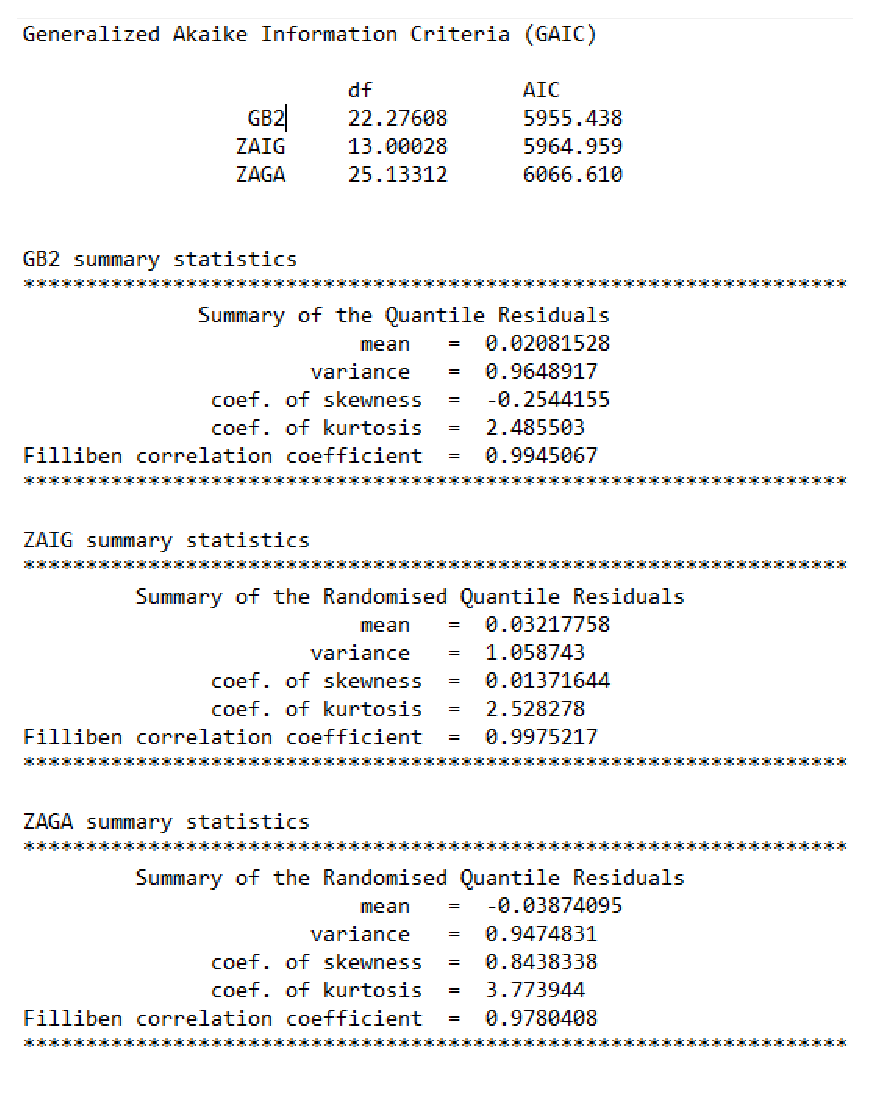
\includegraphics[width=1\linewidth]{GAIC_statistics.eps}
   \caption{}
   \label{Residuals summary statistics} 
\end{subfigure}

\begin{subfigure}[b]{0.5\textwidth}
   \includegraphics[width=1\linewidth]{ROC_4Plot_GB2.eps}
   \caption{}
   \label{Residuals_GB2}
\end{subfigure}

\caption[Normalized quantile residuals from model GB2]{(a)Summary statistics of quantile residuals from models GB2, ZAIG \& ZAGA (b)Displays (normalized quantile) residuals from model $\mbox{GB}2(\mu,\sigma,\nu,\tau)$.}
\end{figure}

\begin{figure}
\centering
\begin{subfigure}[b]{0.5\textwidth}
   \includegraphics[width=1\linewidth]{ROC_4Plot_ZAIG.eps}
   \caption{}
   \label{Residuals_ZAIG} 
\end{subfigure}

\begin{subfigure}[b]{0.5\textwidth}
   \includegraphics[width=1\linewidth]{ROC_4Plot_ZAGA.eps}
   \caption{}
   \label{Residuals_ZAGA}
\end{subfigure}

\caption[Normalized quantile residuals from models ZAIG \& ZAGA]{(a) Display of (normalized quantile) residuals from model $\mbox{ZAIG}(\mu,\sigma,\nu)$ (b) As for (a) but on the model $\mbox{ZAGA}(\mu,\sigma,\nu)$}
\end{figure}

\bibliography{Thesis.bib}


\end{document}
